\documentclass[openany,reqno]{amsbook}
\input ../preamble
\input ../free-macros
\input ../gans.tex
%\newcommand\version{1.1}  \newcommand\semester{Spring 2013}
%\newcommand\version{1.2}   \newcommand\semester{Fall 2013}
%\newcommand\version{1.3}   \newcommand\semester{Fall 2015}
\newcommand\version{1.4}   \newcommand\semester{Fall 2017}
%%%%%%%%%%%%%%%%%%%%%%%%%%%%%%%%%%%%%
%\includeonly{09intapps}
%%%%%%%%%%%%%%%%%%%%%%%%%%%%%%%%%%%%%
\begin{document}
\graphicspath{{../figures/221/}}
%!TEX root =  free221.tex
%%%%%%%%%%%%%%%%%%%%%%%%%%%%%%%%%%%%%%%%%%%%%%%%%%
%%%             THE TITLE PAGE
%%%%%%%%%%%%%%%%%%%%%%%%%%%%%%%%%%%%%%%%%%%%%%%%%%

\includegraphics[width=0.2\textwidth]{UW_logo.png}
\vfill

\begin{flushright}
  \Huge\sffamily\bfseries
  MATH 221 \\
  FIRST SEMESTER \\
  CALCULUS\\[1in]
  \large \semester
\end{flushright}

\vfill
\begin{flushright}
\textsf{Typeset:\today}
\end{flushright}

\newpage
%%%%%%%%%%%%%%%%%%%%%%%%%%%%%%%%%%%%%%%%%%%%%%%%%
\begin{center}
  \bfseries\sffamily MATH 221 -- 1st Semester Calculus \\
  Lecture notes version \version\ (\semester)
\end{center}

\begin{center}
  Copyright (c) 2012 Sigurd B. Angenent, Laurentiu Maxim, Evan Dummit, Joel Robbin.
  Permission is granted to copy, distribute and/or modify this document under
  the terms of the GNU Free Documentation License, Version 1.2 or any later
  version published by the Free Software Foundation; with no Invariant Sections,
  no Front-Cover Texts, and no Back-Cover Texts.  A copy of the license is
  included in the section entitled "GNU Free Documentation License".
\end{center}
\newpage
\sffamily\footnotesize
\begin{multicols}{2}
    \tableofcontents
\end{multicols}

\rmfamily\normalsize



%%%%%%%%%%%%%%%%%%%%%%%%%%%%%%%%%%%%%%%%%%%%%%%%%%%%%%%%%%%%%%%%%%%%%%%%%%%%
% !TEX root =  free221.tex
%%%%%%%%%%%%%%%%%%%%%%%%%%%%%%%%%%%%%%%%%%%%%%%%%%%%%%%%%%%%%%%%%%%%%%%%%%%%

\chapter{Numbers and Functions}


The subject of this course is ``functions of one real variable'' so we
begin by talking about the real numbers, and then discuss functions.


\section{Numbers} 


\subsection{Different kinds of numbers} 
The simplest numbers are the \emph{positive integers}
\[
1, 2, 3, 4,\cdots
\]
the number \emph{zero}
\[
0,
\]
and the \emph{negative integers}
\[
\cdots,-4, -3, -2, -1.
\]
Together these form the integers or ``whole numbers.''



Next, there are the numbers you get by dividing one whole number by another
(nonzero) whole number.  These are the so called fractions or \emph{rational
  numbers}, such as
\[
\frac 12,\, \frac13,\, \frac23,\, \frac 14,\,\frac24,\,
\frac34,\, \frac43,\, \cdots
\]
or
\[
-\frac 12,\, -\frac13,\, -\frac23,\, -\frac 14,\,-\frac24,\,
-\frac34,\, -\frac43,\, \cdots
\]
By definition, any whole number is a rational number (in particular zero is a
rational number.)


You can add, subtract, multiply and divide any pair of rational numbers and the
result will again be a rational number (provided you don't try to divide by
zero).

\marginpar{\footnotesize\sffamily\color{darkbluegreen}%
  Approximating $\sqrt{2}$\,:\rule[-4pt]{0pt}{1pt}\\
  \begin{tabular}{r@{.}lr@{.}ll}
    \toprule
    \multicolumn{2}{c}{$x$}&
    \multicolumn{2}{c}{$x^2$}\\ \midrule
    1&2 & 1&44\\
    1&3 & 1&69\\
    \bfseries\itshape1&\bfseries\itshape4 & \bfseries\itshape1&\bfseries\itshape96&<2\\
    \bfseries\itshape1&\bfseries\itshape5 & \bfseries\itshape2&\bfseries\itshape25&>2\\
    1&6 & 2&56\\
    \bottomrule
  \end{tabular}%
}
There are other numbers besides the rational numbers: it was discovered by the
ancient Greeks that the square root of 2 is not a rational number.  In other
words, there does not exist a fraction $\frac{m}{n}$ such that
\[
\bigl(\frac mn\bigr)^2 = 2, \text{ i.e. }
m^2= 2n^2.
\]
Nevertheless, if you compute $x^2$ for some values of $x$ between $1$ and $2$,
and check if you get more or less than $2$, then it looks like there should be
some number $x$ between $1.4$ and $1.5$ whose square is exactly $2$.

\subsection{A reason to believe in $\sqrt2$} 
The Pythagorean theorem says that the hypotenuse of a right triangle with sides
1 and 1 must be a line segment of length $\sqrt2$.
In middle or high school you learned something similar to the following geometric
construction of a line segment whose length is $\sqrt2$.  Take a square with
side of length 1, and construct a new square one of whose sides is the diagonal
of the first square.  The figure you get consists of 5 triangles of equal area
and by counting triangles you see that the larger square  has exactly twice the
area of the smaller square.
\marginpar{\footnotesize\sffamily%
  
    \begin{picture} (70.000000,70.000000)(0,0)
    \put(0.0, 0.0){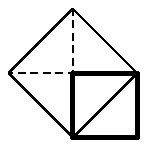
\includegraphics{01smallsquareroot2.pdf}}
    \end{picture}
}
Therefore the diagonal of the smaller square, being
the side of the larger square, is $\sqrt2$ as long as the side of the smaller
square.

So, we will \textit{assume} that there is such a number whose square is exactly
2, and we call it the square root of 2, written as $\sqrt2$.  There are more
than a few questions\footnote{Here are some questions: if we assume into
existence a number a number $x$ between $1.4$ and $1.5$ for which $x^2=2$, how
many other such numbers must we also assume into existence?  How do we know
there is ``only one'' such square root of 2? And how can we be sure that these
new numbers will obey the same algebra rules (like $a+b = b+a$) as the rational
numbers?} raised by assuming the existence of numbers like the square root of 2,
but we will not deal with these questions here.  Instead, we will take a more
informal approach of thinking of real numbers as ``infinite decimal
expansions''.


\subsection{Decimals} 
One can represent certain fractions as finite decimal numbers, e.g.,
\[
\frac{279}{25}= \frac{1116}{100} = 11.16.
\]
Some rational numbers cannot be expressed with a finite decimal expansion.  For instance,
expanding $\frac13$ as a decimal number leads to an unending ``repeating decimal'':
\[
\frac13 = 0.333\,333\,333\,333\,333\,\cdots
\]
It is impossible to write the complete decimal expansion of $\frac13$
because it contains infinitely many digits.  But we can describe the
expansion: each digit is a 3.


Every fraction can be written as a decimal number which may or may
not be finite.  If the decimal expansion doesn't terminate, then it will
repeat (although this fact is not so easy to show).  For instance,
\[
\frac17 = 0.142857\,142857\,142857\,142857\,\dots
\]
Conversely, any infinite repeating decimal expansion represents a
rational number.


A \emph{real number} is specified by a possibly unending decimal
expansion.  For instance,
\[
\sqrt 2 = 1.414\,213\,562\,373\,095\,048\,801\,688\,724\,
209\,698\,078\,569\,671\,875\,376\,9\dots
\]
Of course you can never write \textit{all} the digits in the decimal expansion,
so you only write the first few digits and hide the others behind dots. To
give a precise description of a real number (such as $\sqrt2$) you have to
explain how you could \textit{in principle} compute as many digits in the
expansion as you would like\footnote{What exactly we mean by specifying how to compute digits in decimal expansions of real numbers is another issue that is beyond the scope of this course.}.


\subsection{Why are real numbers called real? } 
All the numbers we will use in this first semester of calculus are ``real
numbers''. At some point in history it became useful to assume that there
is such a thing as $\sqrt{-1}$, a number whose square is $-1$.  No
real number has this property (since the square of any real number is
nonnegative) so it was decided to call this newly-imagined number ``imaginary''
and to refer to the numbers we already had (rationals, $\sqrt2$-like
things) as ``real''.

%!!! Discuss: There are useful things one can do with infinite-number arithmetic, provided one declares things like infinity minus infinity to be undefined.  Students generally want to do these kinds of heuristic calculations anyway, so why not tell them how to do it properly? A revamped discussion would also significantly improve the treatment of infinite limits in the limits chapter.

\subsection{Reasons not to believe in $\infty$} 
\label{sec:infinity-not-a-number}
In calculus we will often want to talk about very large and very small
quantities.  We will use the symbol $\infty$ (pronounced ``infinity'')
all the time, and the way this symbol is traditionally used would suggest that we
are thinking of $\infty$ as just another number.  But $\infty$ is
different.  The ordinary rules of algebra don't apply to $\infty$.  As
an example of the many ways in which these rules can break down, just
think about ``$\infty + \infty$.''  What do you get if you add
infinity to infinity?  The elementary school argument for finding the
sum is: ``if you have a bag with infinitely many apples, and you add
infinitely many more apples, you still have a bag with infinitely many
apples.'' So, you would think that
\[
\infty + \infty = \infty.
\]
If $\infty$ were a number to which we could apply the rules of
algebra, then we could cancel $\infty$ from both sides,
\[
\infty + \not\!\!\infty = \not\!\!\infty \implies \infty = 0.
\]
So infinity is the same as zero!  If that doesn't bother you, then
let's go on.  Still assuming $\infty$ is a number we find that
\[
\frac{\infty}{\infty} = 1,
\]
but also, in view of our recent finding that $\infty = 0$,
\[
\frac{\infty}{\infty} = \frac{0}{\infty} = 0.
\]
Therefore, combining these last two equations,
\[
1=\frac { \infty }{\infty}=0.
\]
In elementary school terms: ``one apple is no apple.''


This kind of arithmetic is not going to be very useful for scientists (or
grocers), so we need to drop the assumption that led to this nonsense,
i.e.\ we have to agree from here on that \footnote{That is not the end of
  the story.  Twentieth century mathematicians have produced a theory of
  ``non standard real numbers'' which includes infinitely large numbers.
  To keep the theory from running into the kind of nonsense we just
  produced, they had to assume that there are many different kinds of
  infinity: in particular $2\times\infty$ is not the same as $\infty$, and
  $\infty\times\infty = \infty^2$ is yet another kind of infinity.  Since
  there are many kinds of infinity in this theory you can't use the single
  symbol ``$\infty$'' because it doesn't say \emph{which} infinitely large
  number you would be talking about.  In this course we will follow the
  traditional standard approach, and assume there are no ``infinitely large
  numbers.'' But if you want to read the version of the theory where
  infinitely large and small numbers do exist, then you should see
  Keisler's calculus text at
  \centerline{\url{http://www.math.wisc.edu/~keisler/calc.html}} }
\begin{center}
  \framebox{ \bfseries\color{badgerred}
  INFINITY IS NOT A NUMBER!}
\end{center}


\subsection{The real number line and intervals} 
It is customary to visualize the real numbers as points on a straight
line.  We imagine a line, and choose one point on this line, which we
call the \emph{origin}.  We also decide which direction we call
``left'' and hence which we call ``right.''  Some draw the number line
vertically and use the words ``up'' and ``down.''

To plot any real number $x$ one marks off a distance $x$ from the
origin, to the right (up) if $x>0$, to the left (down) if $x<0$.

The \emph{distance along the number line} between two numbers $x$ and
$y$ is $|x-y|$.  In particular, the distance is never a negative
number.

\begin{figure}[h]\centering
  
    \begin{picture} (240.000000,39.187500)(0,0)
    \put(0.0, 0.0){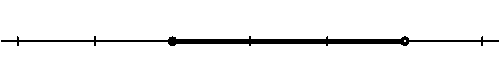
\includegraphics{01drawaninterval.pdf}}
        \put(  6.44,   9.59){\sffamily\itshape $-3$}
    \put( 43.62,   9.59){\sffamily\itshape $-2$}
    \put( 80.81,   9.59){\sffamily\itshape $-1$}
    \put(118.00,   9.59){\sffamily\itshape $0$}
    \put(155.19,   9.59){\sffamily\itshape $1$}
    \put(192.38,   9.59){\sffamily\itshape $2$}
    \put(229.56,   9.59){\sffamily\itshape $3$}
\end{picture}

  \caption{To draw the half open interval $[-1,2)$ use a filled dot to
    mark the endpoint that is included and an open dot for an excluded
    endpoint.  Some like to draw the number line vertically, like a
    thermometer.  }
  \label{fig:01drawaninterval}
\end{figure}
\marginpar{
    \begin{picture} (32.000000,194.000000)(0,0)
    \put(0.0, 0.0){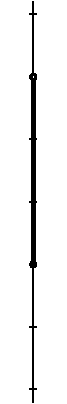
\includegraphics{01drawaninterval-vertical.pdf}}
        \put( 19.00,   7.00){\sffamily\itshape $-3$}
    \put( 19.00,  37.00){\sffamily\itshape $-2$}
    \put( 19.00,  67.00){\sffamily\itshape $-1$}
    \put( 19.00,  97.00){\sffamily\itshape $0$}
    \put( 19.00, 127.00){\sffamily\itshape $1$}
    \put( 19.00, 157.00){\sffamily\itshape $2$}
    \put( 19.00, 187.00){\sffamily\itshape $3$}
\end{picture}
}%

In modern abstract mathematics a collection of real numbers (or any
other kind of mathematical objects) is called a \emph{set}.  Below are
some examples of sets of real numbers.  We will use the notation from
these examples throughout this course.

The collection of all real numbers between two given real numbers forms
an interval.  The following notation is used:
\begin{itemize}
\item $(a,b)$ is the set of all real numbers $x$ that satisfy $a<x<b$.
\item $[a, b)$ is the set of all real numbers $x$ that satisfy $a\leq x<b$.
\item $(a, b]$ is the set of all real numbers $x$ that satisfy $a< x\leq b$.
\item $[a, b]$ is the set of all real numbers $x$ that satisfy $a\leq x\leq b$.
\end{itemize}
If the endpoint is not included then it may be $\infty$ or $-\infty$.
E.g.\ $(-\infty, 2]$ is the interval of all real numbers (both
positive and negative) that are $\leq 2$.

\begin{figure}[t]\centering
  
    \begin{picture} (180.000000,66.727273)(0,0)
    \put(0.0, 0.0){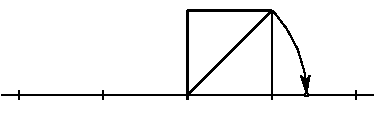
\includegraphics{01root2ontheline.pdf}}
        \put(  7.09,  11.23){\sffamily\itshape $-2$}
    \put( 47.55,  11.23){\sffamily\itshape $-1$}
    \put( 88.00,  11.23){\sffamily\itshape $0$}
    \put(128.45,  11.23){\sffamily\itshape $1$}
    \put(168.91,  11.23){\sffamily\itshape $2$}
\put(147.21,   9.23){$\sqrt2$}
\end{picture}

  \caption{To find $\sqrt2$ on the real line you draw a square of side length
    $1$ and drop the diagonal onto the real line.}
\end{figure}

\subsection{Set notation} 
\label{sec:set-notation}
A common way of describing a set is to say it is the collection of all
    real numbers that satisfy a certain condition.  We use curly braces $\{
    \cdot \}$ to denote sets:
\[
\setA = \bigl\{ x \mid \text{$x$ satisfies this or that condition}\bigr\}
\]
Most of the time we will use upper case letters in a calligraphic font
to denote sets.  ($\setA$,$\setB$,$\setC$,$\setD$, \dots)


For instance, the interval $(a, b)$ can be described as
\[
(a, b) = \bigl\{x \mid a<x<b\bigr\}
\]
The set
\[
\setB = \bigl\{x \mid x^2-1>0\bigr\}
\]
consists of all real numbers $x$ for which $x^2-1>0$, i.e.\ it consists of all
real numbers $x$ for which either $x>1$ or $x<-1$ holds.  This set consists of
two parts: the interval $(-\infty, -1)$ and the interval $(1, \infty)$.

You can try to draw a set of real numbers by drawing the number line and
coloring the points belonging to that set red, or by marking them in some other
way.


Some sets can be very difficult to draw.  For instance,
\[
\setC = \bigl\{x \mid \text{$x$ is a rational number}\bigr\}
\]
can't be accurately drawn.  In this course we will try to avoid such sets.


Sets can also contain a finite collection of numbers which we can simply list, like
\[
\setD = \{1, 2, 3\}
\]
so that $\setD$ is the set containing the numbers 1, 2, and 3.  Or the set
\[
\setE = \bigl\{x \mid x^3-4x^2+1 = 0\bigr\}
\]
which consists of the solutions of the equation $x^3-4x^2+1=0$.
(There are three of them, but it is not easy to give a formula for the
solutions.)


If $\setA$ and $\setB$ are two sets then \emph{the union of $\setA$ and $\setB$}
is the set that contains all numbers that belong either to $\setA$ or to
$\setB$.  The following notation is used
\[
\setA\cup\setB = \bigl\{x \mid
\text{$x$ belongs to $\setA$ or to $\setB$ or both.}\bigr\}
\]
Similarly, the \emph{intersection of two sets $\setA$ and $\setB$} is the set of
numbers that belong to both sets.  This notation is used:
\[
\setA\cap\setB = \bigl\{x \mid
\text{$x$ belongs to both $\setA$ and $\setB$.}\bigr\}
\]
\section{Problems} 
\problemfont 
\begin{multicols}{2}\setlength{\parindent}{0pt}
\problem What is the $2007^{\textit{th}}$ digit after the period in the expansion 
of $\frac17$?
\answer 
The decimal expansion of
\[
1/7 = 0.\overline{142857}\,142857\,142857\,\cdots
\]
repeats after 6 digits.  Since $2007 =
334\times6+3$ the $2007^{\textrm{th}}$ digit is the same as the
$3^{\textrm{rd}}$, which happens to be a $2$.
\endanswer



\problem Which of the following fractions have finite decimal expansions? 
\[
a=\frac 23, \quad b=\frac 3{25},\quad c=\frac{276937}{15625}.
\]


\problem Draw the following sets of real numbers.  Each of these sets is 
the union of one or more intervals.  Find those intervals.  Which of these
sets are finite?



\noindent%
\(\DS\setA = \bigl\{x \mid x^2-3x+2\leq 0\bigr\} \)\\
\(\DS\setB = \bigl\{x \mid x^2-3x+2\geq 0\bigr\}\)\\
\(\DS\setC = \bigl\{x \mid x^2-3x > 3\bigr\} \)\\
\(\DS\setD = \bigl\{x \mid x^2-5>2x\bigr\} \)\\
\(\DS\setE = \bigl\{t \mid t^2-3t+2\leq0\bigr\} \)\\
\(\DS\setF = \bigl\{\alpha \mid \alpha^2-3\alpha+2\geq 0\bigr\}\)\\
\(\DS\setG = (0, 1)\cup (5, 7] \)\\
\(\DS\setH = \bigl( \{1\}\cup\{2,3\} \bigr)\cap (0, 2\sqrt2)\)\\
\(\DS\setQ = \bigl\{\theta \mid \sin\theta=\tfrac12\bigr\} \)\\
\(\DS\setR = \bigl\{\varphi\mid \cos\varphi>0\bigr\}\)
    
% !!! Issue: Is a single element {1} an interval?


\problem Suppose $\setA$ and $\setB$ are intervals.  Is it always true that 
$\setA\cap\setB$ is an interval?  How about $\setA\cup\setB$?




% !!! Issue: Is a single element {1} an interval?  How about the empty set?



\problem Consider the sets 
\[
\setM = \bigl\{x \mid x>0\bigr\} \text{ and }
\setN =  \bigl\{y \mid y>0\bigr\}.
\]
Are these sets the same?
\answer 
Yes these are the same sets.  Both sets consist of all positive real
numbers: since they contain exactly the same numbers, they are the
same sets.
\endanswer
\problem \groupproblem 
Write the numbers
\begin{gather*}
  x=0.3131313131\dots,\\
  y=0.273273273273\dots\\
  \text{ and }
  z=0.21541541541541541\dots
\end{gather*}
as fractions (that is, write them as $\frac mn$, specifying $m$ and
$n$.)


% !!! Issue: This problem is nonsense without a notion of convergent sequence.

(Hint: show that $100x=x+31$. A similar trick works for $y$, but $z$
is a little harder.)
\answer 
$100x = 31.313131\cdots = 31+x \implies 99x = 31 \implies x =
\frac{31}{99}$.

Similarly, $1000y = 273 + y$ so $y= \frac{273}{999}$.

In $z$ the initial ``$2$'' is not part of the repeating pattern, so
subtract it:  $z = 0.2 + 0.0154154154\cdots$.  Now let
$w=0.0154154154\cdots$.  You get $1000w = 15.4+w = 15\frac25 + w =
\frac{77}{5}+w$. Therefore $w= \frac{77}{5\times 999}$.
From this you get
\[
z = \tfrac15+w = \tfrac15 +  \frac{77}{5\times999} = \frac{1076}{4995}.
\]
\endanswer

\problem \groupproblem\label{ex:no-infinitely-small-numbers} 
\subprob In \S\ref{sec:infinity-not-a-number} we agreed that
infinitely large numbers don't exist. Do infinitely small numbers
exist?   In other words, does there exist a \emph{positive} number $x$
that is smaller than $\frac1n$ for all $n=1, 2, 3, 4, \cdots$, i.e.
\begin{gather*}
  0<x<\tfrac{1}{2}, \text{ and }
  0<x<\tfrac{1}{3}, \text{ and } \\
  0<x<\tfrac{1}{4}, \text{ and so on} \cdots?
\end{gather*}

\subprob
Is the number whose decimal expansion after the period consists only
of nines, i.e.
\[
a=0.99999999999999999\dots
\]
the same as the number $1$?  Or could it be that there are numbers
between $0.9999\cdots$ and $1$?  That is, is it possible that there is
some number $x$ that satisfies
\[
0.999999\cdots < x < 1 \; ?
\]

\subprob  Here is a very similar question:  is
\[
b=0.3333333333333333333\dots
\]
the same as $\frac13$?  Or could there be a number $x$ with
\[
0.333333\dots <x<\tfrac13 ?
\]

% !!! Issue: This problem is nonsense without a notion of convergent sequence.
\problem In \S\ref{sec:set-notation} we said that the set 
\[
\setC = \bigl\{x \mid \text{$x$ is a rational number}\bigr\}
\]
was difficult to draw.  Explain why.

\end{multicols}

\noproblemfont%

\section{Functions} 

\subsection{Dependence} 
Calculus deals with quantities that change.  For
instance, the water temperature $T$ of Lake Mendota (as measured at
the pier near the Memorial Union) is a well-defined quantity, but it
changes with time.  At each different time $t$ we will find a
different temperature $T$.  Therefore, when we say ``the temperature at
the pier of Lake Mendota,'' we could mean two different things:   


\begin{itemize}
\item On one hand we could mean the ``temperature at some given
  time,'' e.g.~the temperature at 3pm is 68F: here the temperature is
  just a number.  The most common notation for this is $T(3) = 68$, or
  $T(3\textrm{pm}) = 68\textrm{F}$.

\item On the other hand we could mean the ``temperature in general,''
  i.e.~the temperatures at all times.  In that second interpretation
  the temperature is not just a number, but a whole collection of
  numbers, listing \emph{all} times $t$ and the corresponding
  temperatures $T(t)$.
\end{itemize}


So $T(t)$ is a number while $T$ by itself is not a number, but a more
complicated thing.  It is what in mathematics is called a
\emph{function}.  We say that \textit{the water temperature is a
  function of time.}

Here is the definition of what a mathematical function is:

\subsection{Definition} 
%% eric bach suggests including a comment about computability
%% perhaps a textbox in a figure that raises the question 
%% if the function 
%% f(x) = 1 if the decimal expansion has 200 consecutive zeroes
%%        0 otherwise
%% is well defined.  What is f(pi)?  We do not know all decimals 
%% of pi and we can only compute them one at a time.  If f(pi)=0
%% then the computation that shows this might take infinitely long,
%% i.e. we would never know.
\itshape
To specify a \emph{function} $f$ you must
\begin{enumerate}
\item give a \emph{rule} that tells you how to compute the value $f(x)$ of
  the function for a given real number $x$, and:
\item say for which real numbers $x$ the rule may be applied.
\end{enumerate}%
The set of numbers for which a function is defined is called its \emph{domain}.
The set of all possible numbers $f(x)$ as $x$ runs over the domain is called the
\emph{range} of the function.  The rule must be \emph{unambiguous:} the same
$x$ must always lead to the same $f(x)$.
\upshape

\medskip

For instance, one can define a function $f$ by putting $f(x) = 3x$ for all
$x\geq0$.  Here the rule defining $f$ is ``multiply by 3 whatever
number you're given'', and the function $f$ will accept all real numbers.


The rule that specifies a function can come in many different forms.  Most
often it is a formula, as in the square root example of the previous paragraph.
Sometimes you need a few formulas, as in
\[
g(x) =
\begin{cases}
  2x & \text{for } x<0 \\
  x^2 & \text{for }x\geq0
\end{cases}
\qquad
\text{domain of $g$} = \text{all real numbers.}
\]
Functions whose definition involves different formulas on different
intervals are sometimes called \emph{piecewise defined functions.}

\subsection{Graphing a function} 
  %%% !!! Issue: The Euclidean plane has not been defined!
You get the \emph{graph of a function} $f$ by drawing all points whose
coordinates are $(x,y)$ where $x$ is in the domain of $f$ and $y = f(x)$.
\begin{figure}[h]
  \centering
  
    \begin{picture} (240.000000,144.800000)(0,0)
    \put(0.0, 0.0){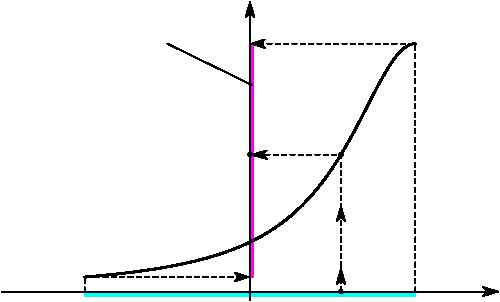
\includegraphics{01graphOFf.pdf}}
        \put( 80.33, 123.97){\sffamily\itshape \makebox[0pt][r]{range of $f$}}
    \put(118.00,  70.71){\sffamily\itshape \makebox[0pt][r]{$y=f(x)$}}
    \put(167.63,  68.71){\sffamily\itshape $(x, f(x))$}
    \put(167.63,   6.97){\sffamily\itshape $x$}
    \put(120.00,  -7.03){\sffamily\itshape \makebox[0pt][c]{domain of $f$}}
\end{picture}

  \caption{The graph of a function $f$. The domain of $f$ consists
    of all $x$ values at which the function is defined, and the range consists
    of all possible values $f$ can have.}
  \label{fig:01graphOFf}
\end{figure}

\begin{figure}[t]
  \centering
  
    \begin{picture} (240.000000,172.000000)(0,0)
    \put(0.0, 0.0){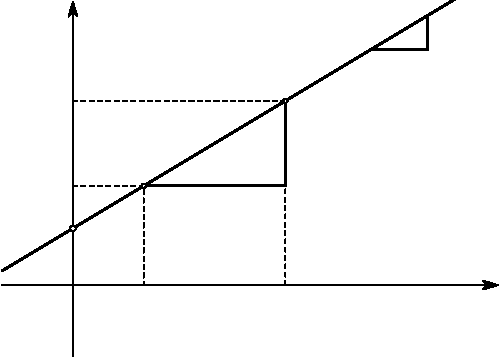
\includegraphics{01line.pdf}}
        \put( 65.00,  90.60){\sffamily\itshape $P_0$}
    \put(133.00, 131.40){\sffamily\itshape $P_1$}
    \put(141.00, 103.00){\sffamily\itshape $y_1-y_0$}
    \put(103.00,  72.60){\sffamily\itshape \makebox[0pt][c]{$x_1-x_0$}}
    \put( 65.00,  23.00){\sffamily\itshape $x_0$}
    \put(133.00,  23.00){\sffamily\itshape $x_1$}
    \put( 25.00,  82.60){\sffamily\itshape $y_0$}
    \put( 25.00, 123.40){\sffamily\itshape $y_1$}
    \put( 33.00,  63.20){\sffamily\itshape \makebox[0pt][r]{$n$}}
    \put(191.40, 139.88){\sffamily\itshape $1$}
    \put(207.00, 155.04){\sffamily\itshape $m$}
\end{picture}

  \caption{The graph of $f(x) = mx+n$ is a straight line.
    It intersects the $y$-axis at height $n$.
    The ratio between the amounts by which $y$ and $x$ increase as you
    move from one point to another on the line is
    $\frac{y_1-y_0}{x_1-x_0} = m$.  This ratio is the same, no matter
    how you choose the points $P_0$ and $P_1$ as long as they are different and on
    the line.}\label{fig:01line}
\end{figure}
\subsection{Linear functions} 
A function $f$ that is given by the formula
\[
f(x) = mx + n
\]
where $m$ and $n$ are constants is called a \emph{linear function}.  Its graph
is a straight line.  The constants $m$ and $n$ are the \emph{slope} and
\emph{$y$-intercept} of the line, respectively.  Conversely, any straight line
which is not vertical (not parallel to the $y$-axis) is the graph of a linear
function.  If we know two points $(x_0, y_0)$ and $(x_1, y_1)$ on the line, then
we can compute the slope $m$ from the ``rise-over-run'' formula
\[
m = \frac{y_1-y_0}{x_1-x_0}.
\]
This formula actually contains a theorem from Euclidean geometry,
namely, it says that the ratio
\[
(y_1-y_0):(x_1-x_0)
\]
is the same for every pair of distinct points $(x_0, y_0)$ and $(x_1, y_1)$
that you could pick on the line.


\subsection{Domain and ``biggest possible domain.'' } 
In this course we will usually not be careful about specifying the
domain of a function.  When this happens the domain is understood to
be the set of all $x$ for which the rule that tells you how to
compute $f(x)$ is a meaningful real number.  For instance, if we say that $h$ is the
function
\[
h(x) = \sqrt x
\]
then the domain of $h$ is understood to be the set of all nonnegative real
numbers
\[
\text{domain of $h$} = [0, \infty)
\]
since $\sqrt x$ is a well-defined real number for all $x\geq 0$ and not a real number for $x<0$.


A systematic way of finding the domain and range of a function for which you are
only given a formula is as follows:
\begin{itemize}
\item The domain of $f$ consists of all $x$ for which $f(x)$ is well-defined
  (``makes sense'')
\item The range of $f$ consists of all $y$ for which you can solve the
  equation $f(x) = y$ to obtain at least one (real) value of $x$.
\end{itemize}


\subsection{Example -- find the domain and range of $f(x) = 1/x^2$} 
The expression $1/x^2$ can be computed for all real numbers $x$ except
$x=0$ since this leads to division by zero.  Hence the domain of the
function $f(x) = 1/x^2$ is
\[
\text{``all real numbers except $0$''}
=\bigl\{x \mid x\neq0\bigr\} = (-\infty, 0)\cup(0, \infty).
\]
To find the range we ask ``for which $y$ can we solve the equation
$y=f(x)$ for $x$,'' i.e.\ for which $y$ can we solve $y=1/{x^2}$ for
$x$?


If $y=1/x^2$ then we must have $x^2 = 1/y$, so first of all, since we
have to divide by $y$, $y$ can't be zero.  Furthermore, $1/y=x^2$ says
that $y$ must be positive.  On the other hand, if $y>0$ then $y=1/x^2$
  has a solution (in fact two solutions), namely $x=\pm1/\sqrt{y}$.  This
shows that the range of $f$ is
\[
\text{``all positive real numbers''} = \{x \mid x>0\} = (0, \infty).
\]
\subsection{Functions in ``real life''} 
One can describe the motion of an object using a function.  If some
object is moving along a straight line, then you can define the
following function: Let $s(t)$ be the distance from the object to a
fixed marker on the line, at the time $t$.  Here the domain of the
function is the set of all times $t$ for which we know the position of
the object, and the rule is
\begin{center}
  \itshape Given $t$, measure the distance between the object at time $t$ and the
  marker.
\end{center}
\smallskip
\centerline{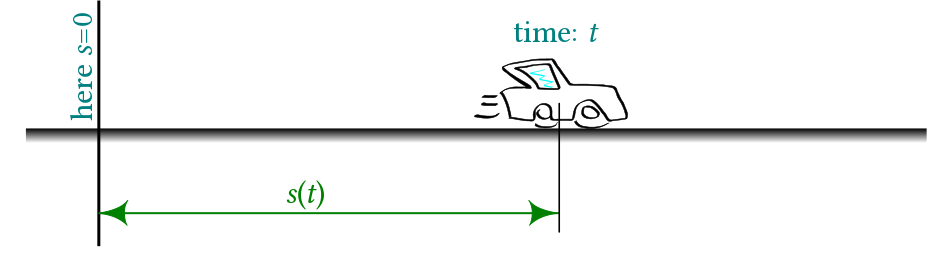
\includegraphics[width=0.6\textwidth]{01car.png}}%
There are many examples of this kind.  For instance, a biologist could
describe the growth of a mouse by defining $m(t)$ to be the mass of the mouse
at time $t$ (measured since the birth of the mouse).  Here the domain is the
interval $[0, T]$, where $T$ is the lifespan of the mouse, and the rule
that describes the function is
\begin{center}
  \itshape Given $t$, weigh the mouse at time $t$.
\end{center}


\marginpar{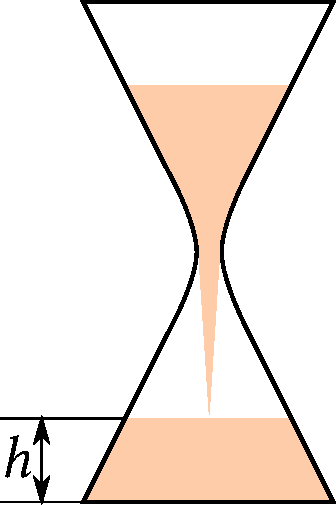
\includegraphics[width=48pt]{01hourglass.pdf}}%
  % !!! Pedantic issue: Sand falling an hourglass doesn't actually look like this.
Here is another example: suppose you are given an hourglass.  If you turn
it over, then sand will pour from the top part to the bottom part.  At any
time $t$ you could measure the height of the sand in the bottom and
call it $h(t)$.  Then, as in the previous examples, you can say that the height of
the sand is a function of time.  But in this example you can let the two
variables height and time switch roles: given a value for $h$ you wait
until the pile of sand in the bottom has reached height $h$ and check what
time it is when that happens: the resulting time $t(h)$ is determined by
the specified height $h$.  In this way you can regard time as a function of
height.




\subsection{The Vertical Line Property} 
Generally speaking, graphs of functions are curves in the plane but
they distinguish themselves from arbitrary curves by the way they
intersect vertical lines: \emph{The graph of a function cannot
intersect a vertical line ``$x=\text{\em constant}$'' in more than one
point}.  The reason why this is true is very simple: if two points lie
on a vertical line, then they have the same $x$ coordinate, so if they
also lie on the graph of a function $f$, then their $y$-coordinates
must both be equal to $f(x)$, so in fact they are the same point.



\subsection{Example -- a cubic function} 
The graph of $f(x) = x^3-x$ ``goes up and down,'' and, even though it
intersects several horizontal lines in more than one point, it
intersects every vertical line in exactly one point.  See
Figure~\ref{fig:01horizontal-and-vertical-line-tests}.
  % !!! Issue: The horizontal line test is not mentioned in the text!




\begin{figure}[t]\centering
  
    \begin{picture} (240.000000,104.000000)(0,0)
    \put(0.0, 0.0){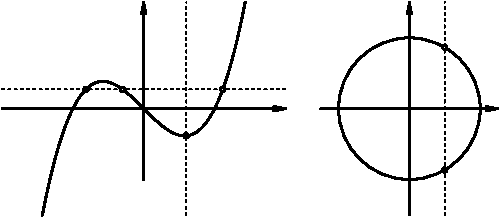
\includegraphics{01cubicANDcircle.pdf}}
        \put( 24.80,   9.50){\sffamily\itshape $y=x^3-x$}
\end{picture}
%
  \caption{The graph of $y=x^3-x$ fails the ``horizontal line test,'' but it
    passes the ``vertical line test.''  The circle fails both tests.}
  \label{fig:01horizontal-and-vertical-line-tests}
\end{figure}

\subsection{Example -- a circle is not a graph of a function $y=f(x)$} 
\label{sec:01circle-izno-graph}
The collection of points determined by the equation $x^2+y^2=1$ is a circle.  It
is not the graph of a function since the vertical line $x=0$ (the $y$-axis)
intersects the graph in two points $P_1(0,1)$ and $P_2(0,-1)$. See again
Figure~\ref{fig:01horizontal-and-vertical-line-tests}.  This example
continues in \S~\ref{sec:implicit-example-h1h2h3} below.


\section{Implicit functions} 
    % !!! Terminology: We should call these things implicit relations, not implicit
    % functions. This fixes a lot of annoying pedantic issues, particularly with
    % talking about the domain. The correct notion to introduce is not whether an
    % implicit relation globally defines a function, but whether it locally defines
    % one. (Even this, nobody really cares much about.)
    % This section needs a lot of wording fixes.
For many functions the rule that tells you how to compute it is not an explicit
formula, but instead an equation that you still must solve.  A function that is
defined in this way is called an ``implicit function.''  


\subsection{Example} 
We can define a function $f$ by saying that if $x$ is any given number,
then $y = f(x)$ is the solution of the equation
\[
x^2+2y-3=0.
\]
In this example we can solve the equation for $y$,
\[
  y = \frac{3-x^2}{2}.
\]
Thus we see that the function we have defined is $f(x) = (3-x^2)/2$.

Here we have two definitions of the same function, namely
\begin{itemize}
\item [(i)] ``$y=f(x)$ is defined by $x^2+2y-3=0$,'' and
\item [(ii)] ``$f$ is defined by $f(x) = (3-x^2)/2$.''
\end{itemize}
The first definition is an implicit definition, the second is explicit.
This example shows that with an ``implicit function'' it is not the
function itself, but rather the way it was defined that is implicit.

\subsection{Another example: domain of an implicitly defined function} 
Define $g$ by saying that for any $x$ the value $y=g(x)$ is the
solution of
\[
  x^2+xy-3=0.
\]
Just as in the previous example you can then solve for $y$, and you
find that
\[
  g(x) = y = \frac{3-x^2}x.
\]
Unlike the previous example this formula does not make sense when $x=0$, and
indeed, for $x=0$ our rule for $g$ says that $g(0) = y$ is the solution of
\[
  0^2+0\cdot y-3=0, \text{ i.e. $y$ is the solution of }3=0.
\]
That equation has no solution and hence $x=0$ does not belong to the domain
of our function $g$.  

\begin{figure}[h]
  \centering
  
    \begin{picture} (360.000000,109.400000)(0,0)
    \put(0.0, 0.0){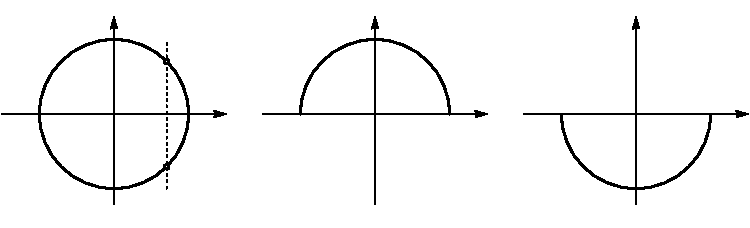
\includegraphics{01circle.pdf}}
        \put( 40.38,  90.50){\sffamily\itshape \makebox[0pt][r]{$x^2+y^2=1$}}
    \put(208.31,  84.01){\sffamily\itshape $y=+\sqrt{1-x^2}$}
    \put(333.61,  23.39){\sffamily\itshape $y=-\sqrt{1-x^2}$}
\end{picture}

  \caption{The circle determined by $x^2+y^2=1$ is not the graph of a
  function, but it contains the graphs of the two functions
  $h_1(x) = \sqrt{1-x^2}$ and $h_2(x)= -\sqrt{1-x^2}$.}
  \label{fig:01circle}
\end{figure}


\subsection{Example: the equation alone does not determine the function} 
% !!! this entire section is useless, pedantic hairsplitting
\label{sec:implicit-example-h1h2h3}
We saw in \S~\ref{sec:01circle-izno-graph} that the unit circle is not
the graph of a function (because it fails the vertical line test).
What happens if you ignore this fact and try to use the equation
$x^2+y^2=1$ for the circle to define a function anyway?
To find out, suppose we define $y=h(x)$ to be ``the solution'' of
\[
  x^2 + y^2=1.
\]
If $x>1$ or $x<-1$ then $x^2>1$ and there is no solution, so $h(x)$ is
at most defined when $-1\leq x\leq 1$.  But when $-1<x<1$ there is
another problem: not only does the equation have a solution, it
has \emph{two} solutions:
\[
  x^2+y^2=1 \iff y = \sqrt{1-x^2} \text{ or } y=-\sqrt{1-x^2}.
\]
The rule that defines a function must be unambiguous, and since we
have not specified which of these two solutions is $h(x)$ the function
is not defined for $-1<x<1$.



Strictly speaking, the domain of the function that is defined implicitly by
the equation $x^2+y^2=1$ consists of only two points, namely $x=\pm1$.
Why?  Well, those are the only two values of $x$ for which the equation has
exactly one solution $y$ (the solution is $y=0$.)  To see this in the
picture, look at Figure~\ref{fig:01circle} and find all vertical lines that
intersect the circle on the left exactly once.  


To get different functions that are described by the equation $x^2+y^2=1$,
we have to specify for each $x$ which of the two solutions
$\pm\sqrt{1-x^2}$ we declare to be ``$f(x)$''.  This leads to many possible
choices.  Here are three of them:
\begin{align*}
  h_1(x) & = \text{the non negative solution $y$ of } x^2+y^2=1 \\
  h_2(x) & = \text{the non positive solution $y$ of } x^2+y^2=1 \\
  h_3(x) & =
  \begin{cases}
    h_1(x) & \text{when $x<0$} \\
    h_2(x) & \text{when $x\geq0$} \\
  \end{cases}
\end{align*}
There are many more possibilities.



\subsection{Why and when do we use implicit functions? Three examples} 
% None of these examples is useful or gives any motivation for why implicit relations are necessary.
\label{sec:why-implicit}
In all the examples we have done so far we could replace the implicit
description of the function with an explicit formula.  This is not always
possible, or, even if it is possible, then the implicit description can still be much
simpler than the explicit formula.



As a first example, define a function $f$ by saying that $y=f(x)$ if
and only if $y$ is the largest of the solutions of
\begin{equation}\label{eq:01quadratic-implicit}
  y^2+3y+2x = 0.
\end{equation}
This means that the recipe for computing $f(x)$ for any given $x$ is ``solve the
equation $y^2+3y+2x = 0$ for $y$ and, if the solutions are real numbers, then
set $y$ equal to the largest solution you find.''  For example, to compute
$f(0)$, we set $x=0$ and solve $y^2+3y=0$.  By factoring $y^2+3y = (y+3)y$, we
find that the solutions are $y=0$ and $y=-3$.  Since $f(0)$ is defined to be the
\textit{largest} of the solutions, we get $f(0)=0$.  Similarly, to compute
$f(1)$ we solve $y^2+3y +2\cdot1=0$: the solutions are $y=-1$ and $y=-2$, so
$f(1) = -1 $.  For any other $x\leq \frac{9}{8}$ the quadratic formula tells us
that the solutions are
\[
  y = \frac{-3 \pm \sqrt{3^2-4\cdot 2x}} {2} = \frac{-3\pm\sqrt{9-8x}} {2}.
\]
By definition $f(x)$ is the largest solution, so
\[
  f(x) = -\frac{3} {2} + \frac{1} {2}\sqrt{9-8x} \, .
\]
If you don't like square roots, then the equation
\eqref{eq:01quadratic-implicit} looks a lot simpler than this formula,
and you would prefer to work with \eqref{eq:01quadratic-implicit}.



For a more extreme example, suppose you were asked to work with a
function $g$ defined implicitly by
\begin{equation}\label{eq:01cubic-implicit}
  y=g(x) \text{ if and only if } y^3+3y+2x = 0.
\end{equation}
This equation is a cubic equation and it is much harder to solve than the
quadratic equation we had before.  It turns out that for any value of $x$, there
is exactly one real value of $y$ for which $y^3+3y+2x=0$, and the solution was
found in the early 1500s by Cardano and Tartaglia \footnote{The solution was
actually found by Tartaglia and, according to some, stolen by Cardano.  To see
the solution and its history you can check the internet, and, in particular, the
Wikipedia pages on Cardano and Tartaglia.}.  Here it is :
\[
  y = g(x) = \sqrt[3]{-x+\sqrt{1+x^2}}-\sqrt[3]{x+\sqrt{1+x^2}}.
\]
Don't worry about how this formula came about; let's just trust
Cardano and Tartaglia.  The implicit description
\eqref{eq:01cubic-implicit} looks a lot simpler, and when we try to
differentiate this function later on, it will be much easier to use
``implicit differentiation'' than to use the Cardano-Tartaglia formula
directly.

Finally, you could have been given the function $h$ whose definition is
\begin{equation}\label{eq:01transcendental-implicit}
  y=h(x) \text{ if and only if } \sin(y)+3y+2x = 0.
\end{equation}
There is no formula involving only standard functions (exponents, trig
and inverse trig functions, logarithms, etc.~for the solution to this
equation.  Nonetheless it turns out that no matter how you choose $x$,
the equation $\sin(y)+3y+2x=0$ has exactly one solution $y$; in fact,
you will prove this in Problem~\ref{ex:implicit-from-ch1}.  So the
function $h$ is well defined, but for this function the implicit
description is the only one available.




\section{Inverse functions} 
If we have a function $f$, which takes input values and sends them to an output,
we might want to try to define a function $f^{-1}$ which ``undoes'' $f$, by the
following prescription:
\begin{equation}\label{eq:rule-for-inverse}
  \parbox{0.7\textwidth}{\centering\itshape%
  For any given $x$ we say that $y = f^{-1}(x)$\\[1pt]
    if $y$ is the solution of $f(y)=x$.}
\end{equation}
Note that $x$ and $y$ have swapped their usual places in this last equation!

The prescription \eqref{eq:rule-for-inverse} defines the inverse function
$f^{-1}$, but it does not say what the domain of $f^{-1}$ is.  By definition,
\textit{the domain of $f^{-1}$ consists of all numbers $x$ for which the
  equation $f(y) = x$ has \emph{exactly one} solution.} ` So if for some $x$ the
equation $f(y)=x$ has no solution $y$, then that value of $x$ does not belong to
the domain of $f^{-1}$.

If, on the other hand, for some $x$ the equation $f(y)=x$ has \textit{more than
  one} solution $y$, then the prescription \eqref{eq:rule-for-inverse} for
computing $f^{-1}(x)$ is ambiguous: which of the solutions $y$ should be
$f^{-1}(x)$?  When this happens we throw away the whole idea of finding the
inverse of the function $f$, and we say that the inverse function $f^{-1}$ is
undefined (``the function $f$ has no inverse''.)


\begin{figure}[b]
    \centering 
    \begin{picture} (300.000000,132.375000)(0,0)
    \put(0.0, 0.0){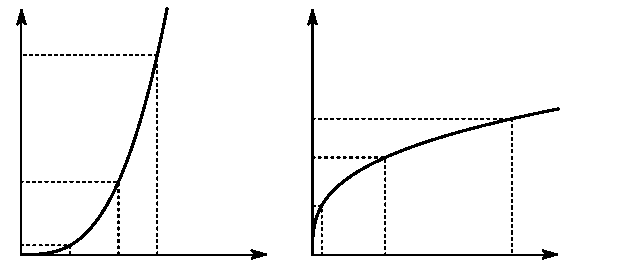
\includegraphics{01inversefunctions.pdf}}
        \put( 33.59,   0.31){\sffamily\itshape \makebox[0pt][c]{$a$}}
    \put(  8.31,  14.68){\sffamily\itshape \makebox[0pt][r]{$f(a)$}}
    \put(154.37,   0.31){\sffamily\itshape \makebox[0pt][c]{$f(a)$}}
    \put(148.00,  33.59){\sffamily\itshape \makebox[0pt][r]{$a$}}
    \put( 56.88,   0.31){\sffamily\itshape \makebox[0pt][c]{$b$}}
    \put(  8.31,  45.23){\sffamily\itshape \makebox[0pt][r]{$f(b)$}}
    \put(184.92,   0.31){\sffamily\itshape \makebox[0pt][c]{$f(b)$}}
    \put(148.00,  56.88){\sffamily\itshape \makebox[0pt][r]{$b$}}
    \put( 75.50,   0.31){\sffamily\itshape \makebox[0pt][c]{$c$}}
    \put(  8.31, 106.14){\sffamily\itshape \makebox[0pt][r]{$f(c)$}}
    \put(245.83,   0.31){\sffamily\itshape \makebox[0pt][c]{$f(c)$}}
    \put(148.00,  75.50){\sffamily\itshape \makebox[0pt][r]{$c$}}
    \put( 14.97, 131.38){\sffamily\itshape The graph of $f$}
    \put(163.97,  94.12){\sffamily\itshape The graph of $f^{-1}$}
\end{picture}

    \caption{The graph of a function and its inverse are mirror images of each
      other.  Can you draw the mirror?}
    \label{fig:function-with-inverse}
\end{figure}


\subsection{Example -- inverse of a linear function}
Consider the function $f$ with $f(x)=2x+3$.  Then the equation $f(y) = x$ works
out to be
\[
2y+3=x
\]
and this has the solution
\[
y=\frac{x-3}2.
\]
So $f^{-1}(x)$ is defined for all $x$, and it is given by $f^{-1}(x) = (x-3)/2$.

\subsection{Example -- inverse of $f(x) = x^2$}
It is often said that ``the inverse of $x^2$ is $\sqrt{x}$.{}'' This is not
quite true, as you'll see in this and the next example.


Let $f$ be the function $f(x) = x^2$ with domain all real numbers.  What is
$f^{-1}$?

The equation $f(y) = x$ is in this case $y^2=x$.  When $x>0$ the equation has
two solutions, namely $y=+\sqrt{x} $ and $y = -\sqrt{x}$.  According to our
definition, the function $f$ does not have an inverse.

\subsection{Example -- inverse of $x^2$, again}
\label{sec:inverse-of-square}%
Consider the function $g(x) = x^2$ with domain all \emph{positive} real numbers.
To see for which $x$ the inverse $g^{-1}(x)$ is defined we try to solve the
equation $g(y) =x$, i.e.\ we try to solve $y^2 = x$.  If $x<0$ then this
equation has no solutions since $y^2\geq0$ for all $f$.  But if $x\geq 0$ then
$y^2 = x$ does have a solution, namely $y = \sqrt{x}$.

So we see that $g^{-1}(x)$ is defined for all positive real numbers $x$, and
that it is given by $g^{-1}(x) = \sqrt x$.

This example is shown in Figure~\ref{fig:function-with-inverse}.  See also
Problem~\ref{ex:inverse-of-square}.


\begin{figure}[b]
  \centering \input{../figures/221/01arcsine-arctan-definition.pdf_tex}
  \caption{Definition of $\arcsin x$ and $\arctan x$.  The dotted circles are
    unit circles.  On the left a segment of length $x$ and its arc sine are
    drawn.  The length of the arc drawn on the unit circle is the subtended
    angle in radians, i.e.~$\arcsin x$.  So $\arcsin x$ is the length of ``the
    arc whose sine is $x$.''}
  \label{fig:01arcsine-arctan-definition}
\end{figure}

\section{Inverse trigonometric functions}
The two most important inverse trigonometric functions are the \emph{arcsine}
and the \emph{arctangent}.  The most direct definition of these functions is
given in Figure~\ref{fig:01arcsine-arctan-definition}.  In words, $\theta =
\arcsin x$ is the angle (in radians) whose sine is $x$.  If $-1\leq x\leq 1$
then there always is such an angle, and, in fact, there are many such angles.
To make the definition of $\arcsin x$ unambiguous we always choose $\theta$ to
be the angle that lies between $-\frac\pi2$ and $+\frac\pi2$.  To see where the
name ``arcsine'' comes from, look at
Figure~\ref{fig:01arcsine-arctan-definition} on the left.


An equivalent way of defining the arcsine and arctangent is to say that they are
the inverse functions of the sine and tangent functions on a restricted domain.
E.g.~if $y=f(x) = \sin x$, then the inverse of the function $f$ is by definition
(see \eqref{eq:rule-for-inverse}) the function $f^{-1}$ with the property that
\[
y =f^{-1}(x) \iff x = f(y) = \sin y.
\]
If we restrict $y$ to the interval $-\frac\pi2\leq y \leq \frac\pi2$ then this
is just the definition of $\arcsin x$, so
\[
y =\sin x \iff x=\arcsin y, \quad \text{provided } -\tfrac\pi2 \leq x\leq \tfrac
\pi2.
\]
Likewise,
\[
y =\tan x \iff x=\arctan y, \quad \text{provided } -\tfrac\pi2 \leq x\leq \tfrac
\pi2.
\]
Forgetting about the requirement that $-\frac\pi2 \leq x\leq \frac \pi2$ can
lead to unexpected mistakes (see Problem~\ref{ex:01sine-of-arcsine}).

\begin{figure}[t]
  \begin{center}
    \parbox{0.6\textwidth}{\input ../figures/221/01sine.tex}%
    \parbox{0.38\textwidth}{\input ../figures/221/01arcsine.tex}\\
    \parbox{0.6\textwidth}{\input ../figures/221/01tangent.tex}%
    \parbox{0.38\textwidth}{\input ../figures/221/01arctangent.tex}
  \end{center}
  \caption{The graphs of the sine and tangent functions on the left, and their
    inverses, the arcsine and arctangent on the right.  Note that the graph of
    arcsine is a mirror image of the graph of the sine, and that the graph of
    arctangent is a mirror image of the graph of the tangent.  }
  \label{fig:01sine-and-arcsine}
\end{figure}%


Because of the interpretation of $y=\arcsin x$ as the inverse of the sine
function, the notations
\[
\arcsin x = \sin^{-1} x,\qquad \arctan x = \tan^{-1} x
\]
are very commonly used.

In addition to the arcsine and arctangent, people have also defined the
arccosine, the arcsecant and the arccosecant.  However, because they can all be
expressed in terms of the arcsine and arctangent, we will not bother with them.

\section{Problems}
\problemfont%

\begin{multicols}{2}\setlength{\parindent}{0pt}
\problem The functions $f$ and $g$ are defined by 
\[
    f(x) = x^2 \text{ and } g(s) = s^2.
\]
Are $f$ and $g$ the same functions or are they different?
\answer 
  They are the same function.  Both are defined for all real numbers,
  and both will square whatever number you give them, so they are the
  same function.
\endanswer


\problem Find a formula for the function $f$ that is defined by 
\[
  y=f(x) \iff x^2y+y = 7.
\]
What is the domain of $f$?


\problem Find a formula for the function $f$ that is defined by the 
requirement that for any $x$ one has
\[
  y=f(x) \iff x^2y-y = 6.
\]
What is the domain of $f$?


\problem Let $f$ be the function defined by the requirement that for 
any $x$ one has
\[
  y=f(x) \iff \parbox{96pt}{\raggedright$y$ is the largest of all\\
  possible solutions of\\ $y^2 = 3x^2-2xy$.}
\]
Find a formula for $f$.  What are the domain and range of $f$?
\answer 
Let $x$ be any number.  Then, $f(x)$, if it is defined, is the largest

\endanswer


\problem Find a formula for the function $f$ that is defined by 
\[
  y=f(x) \iff
  \parbox{96pt}{\centering$2x+2xy+y^2 = 5$\\ and  $y>-x$.}
\]
Find the domain of $f$.

\problem\label{ex:inverse-of-square} 
(continuation of example~\ref{sec:inverse-of-square}.)
Let $k$ be the function with $k(x) = x^2$ whose domain is all \textit{negative}
real numbers. Find the domain of $k^{-1}$, and draw the graph of $k^{-1}$.
\answer 
The domain of $k^{-1} $ is $(0, \infty)$, and $k^{-1}(x) = -\sqrt{x}$.
\endanswer

\problem Use a calculator to compute $g(1.2)$ in three decimals where $g$ 
is the implicitly defined function from \S\ref{sec:why-implicit}.  (There
are (at least) two different ways of finding $g(1.2)$)

\problem \label{ex:01sine-of-arcsine} \groupproblem 
\textbf{True or false?}

\subprob For all real numbers $x$ one has
\[
  \sin\bigl(\arcsin x\bigr) = x.
\]
\answer 
False: Since $\arcsin x$ is only defined if $-1\leq x\leq 1$ and hence
not for \emph{all} $x$, it is not true that $\sin\bigl(\arcsin
x\bigr) = x$ for \emph{all} real numbers $x$.
However, it is true that $\sin(\arcsin x) = x$ for all $x$ in
the interval $[-1,1]$.
\endanswer
\subprob For all real numbers $x$ one has
\[
  \arcsin\bigl(\sin x\bigr) = x.
\]
\answer 
$\arcsin(\sin x)$ is defined for all $x$ since $\sin x$ is
defined for all $x$, and $\sin x$ is always between $-1$ and $1$.
However the arcsine function always returns a number (angle) between
$-\pi/2$ and $\pi/2$, so $\arcsin( \sin x) = x$ can't be true when
$x>\pi/2$ or $x<-\pi/2$.  For $|x|\leq \pi/2$ it is true that $\arcsin
\sin x = x$.
\endanswer
\subprob For all real numbers $x$ one has
\[
  \arctan\bigl( \tan x\bigr) = x.
\]
\answer 
Again, not true: if $x=\pi/2$ then $\tan x$ is not defined and therefore
$\arctan(\tan x)$ is not defined either.


Apart from that, $\arctan (\text{anything})$ always lies
between $-\pi/2 $ and $+\pi/2$, so $\arctan(\tan x)$ cannot
be the same as $x$ if either $x>\pi/2$ or $x<-\pi/2$.
\endanswer
\subprob For all real numbers $x$ one has
\[
  \tan\bigl( \arctan x\bigr) = x.
\]
\answer 
True.
\endanswer


\problem On a graphing calculator plot the graphs of the following 
functions, and explain the results. (Hint: first do the previous exercise.)
\begin{align*}
  f(x) &= \arcsin(\sin x),  &  -2\pi\leq x\leq 2\pi \\
  g(x) &= \arcsin(x) + \arccos(x),  &  0\leq x\leq 1 \\
  h(x) &= \arctan\frac{\sin x}{\cos x},  &  |x|< \pi/2 \\
  k(x) &= \arctan\frac{\cos x}{\sin x},  &  |x|< \pi/2 \\
  l(x) &= \arcsin(\cos x),  &  -\pi\leq x\leq \pi \\
  m(x) &= \cos(\arcsin x), & -1\leq x\leq 1
\end{align*}


% !!! Issue: Arccos is not defined!



\problem Find the inverse of the function $f$ that is given by $f(x) = 
\sin x$ and \emph{whose domain is }$\pi\leq x\leq 2\pi$.  Sketch the graphs
of both $f$ and $f^{-1}$.


\problem Find a number $a$ such that the function $f(x) = \sin(x+\pi/4)$ 
with domain $a\leq x\leq a+\pi$ has an inverse.  Give a formula for
$f^{-1}(x)$ using the arcsine function.


\problem Simplicio has found a new formula for the arcsine.  His reasoning 
is as follows:


{\itshape
Since everybody writes ``the square of $\sin y$'' as
\[
  \bigl(\sin y\bigr)^2 = \sin^2 y.
\]
we can replace the $2$'s by $-1$'s and we get
\[
  \arcsin y = \sin^{-1}y
  =
  \bigl(\sin y\bigr)^{-1} = \frac 1{\sin y}.
\]}%
Is Simplicio right or wrong?  Explain your opinion.




\problem Draw the graph of the function $h_3$ from 
\S\ref{sec:implicit-example-h1h2h3}.



\problem A function $f$ is given that satisfies 
\[
  f(2x+3) = x^2
\]
for all real numbers $x$.

If $x$ and $y$ are arbitrary real numbers
then compute



\subprob $f(0)$
\answer 
Set $x=-3/2$ in $f(2x+3) = x^2$ and you find $f(0) = (-3/2)^2 =
\frac{9}{4}$.
\endanswer



\subprob $f(3)$
\answer 
Set $x=0$ in $f(2x+3) = x^2$ and you find $f(3) = 0^2 = 0$.
\endanswer

\subprob $f(\pi)$
\answer 
Solve $2x+3 = \pi$ for $x$:  $x=\frac{\pi-3}{\pi}$.  Substitute this in $f(2x+3) =
x^2$ and you find $f(\pi) = \bigl(\frac{\pi-3}{2}\bigr)^2$.
\endanswer

\subprob $f(t)$
\answer 
Solve $2x+3 = t$ for $x$:  $x=\frac{t-3}{2}$.  Substitute this in $f(2x+3) =
x^2$ and you find $f(t) = \bigl(\frac{t-3}{2}\bigr)^2$.
\endanswer


\subprob $f(x)$
\answer 
From the previous problem we know what $f(t)$ is for any $t$ so just substitute $t=x$:
$f(x)= b\bigl(\frac{x-3}{2}\bigr)^2$.




\endanswer
\subprob $f(f(2))$
\answer 
$f(2) = \bigl((2-3)/2\bigr)^2 = \frac{1}{4}$.
\endanswer


\subprob $f(2f(x))$
\answer 
$f(2f(x)) = \bigl(\frac{2f(x)-3}{2}\bigr)^2 =
\Bigl\{\frac{2\bigl(\frac{x-3}{2}\bigr)^2 - 3}{2}\Bigr\}^2$.



\endanswer







\problem A function $f$ is given that satisfies 
\[
  f\bigl(\frac1{x+1}\bigr) = 2x-12
\]
for all real numbers $x$.

If $x$ and $t$ are arbitrary real numbers, then
compute the following quantities:

\subprob $f(1)$
\answer 
We know $f\bigl(\frac1{x+1}\bigr) = 2x-12$ for all $x$, so if we want to know
$f(1)$ then we have to find an $x$ with $\frac{1}{x+1} = 1$.  Solving $\frac{1}{x+1} = 1$
for $x$ you find $x=0$. Substitute $x=0$ in $f\bigl(\frac1{x+1}\bigr) = 2x-12$
and you get $f(1) = 2\times0-12 = -12$.
\endanswer


\subprob $f(0)$
\answer 
To find $f(0)$ you proceed as above, this time solving $\frac{1}{x+1} = 0$ for
$x$.  In this case there is no solution $x$, and therefore the equation
$f\bigl(\frac1{x+1}\bigr) = 2x-12$ does not tell us what $f(0)$ is.  Conclusion:
either 0 is not in the domain of $f$, or we cannot tell what $f(0)$ is from
the  information provided in the problem.
\endanswer



\subprob $f(t)$
\answer 
To find $f(t)$ you do the same as when you want to find $f(1)$.
We know $f\bigl(\frac1{x+1}\bigr) = 2x-12$ for all $x$, so if we want to know
$f(t)$ then we have to find an $x$ with $\frac{1}{x+1} = t$.  Solving $\frac{1}{x+1} = t$
for $x$ you find $x=\frac 1t -1$. Substitute $x=\frac 1t -1$ in $f\bigl(\frac1{x+1}\bigr) = 2x-12$
and you get $f(t) = 2\times\bigl(\frac{1}{t}-1\bigr)-12 = \frac{2}{t} -14 $.
\endanswer


\subprob $f(x)$
\answer 
$f(2f(x)) = \frac{2}{2f(x)} - 14 = \frac{1}{f(x)} - 14 =
\frac{1}{\frac{2}{x}-14} - 14$.  You could simplify this if you wanted to, but
that was not part of the question.
\endanswer



\subprob $f(f(2))$
\answer 
After finding $f(t) = \frac{2}{t} -14 $ you can substitute $t=x$ and you find
$f(x) = \frac{2}{x} -14 $.
\endanswer



\subprob $f(2f(x))$
\answer 
$f(2) = \frac{2}{2}-14 = -13 $ and therefore $f(f(2)) = f(-13) = \frac{2}{-13}-14 = -14\frac2{13} $.
\endanswer




\problem Does there exist a function $f$ that satisfies 
\[
  f(x^2) = x+1
\]
for \emph{all} real numbers $x$?
\answer 
No.  For instance if you set $x=1$ you get $f(1) = 1+1=2$, and if you set
$x=-1$ then you get $f((-1)^2) = (-1)+1$, i.e.\ $f(1) = 0$.  But $f(1)$
can't be equal to both $2$ and $0$, the formula $f(x^2) = x+1$ cannot be
true for all real numbers $x$.
\endanswer




\[
  *\; *\; *\;
\]
\noindent\itshape%
The following exercises review precalculus material involving quadratic
expressions $ax^2+bx+c$ in one way or another.\upshape



\problem Find the vertex $(h,k)$ of the parabola $y=ax^2+bx+c$.  Use the result 
to find the range of this function.  Note that the behavior depends on whether
$a$ is positive or negative.  (Hint: ``Complete the square'' in the quadratic
expression by writing it in the form $y=a(x-h)^2 + k$ for some $h$ and $k$ in
terms of $a$, $b$, and $c$.)



\problem Find the ranges of the following functions: 
\begin{align*}
  f(x) &= 2x^2+3 \\
  g(x) &= -2x^2+4x \\
  h(x) &= 4x +x^2\\
  k(x) &= 4\sin x + \sin^2 x \\
  \ell(x) &= 1/(1+x^2)\\
  m(x) &= 1/(3+2x+x^2).
\end{align*}
\answer 
$g(x) = -2\bigl(x^2-2x\bigr)
= -2\bigl(x^2-2x+1 -1\bigr)
= -2\bigl[(x-1)^2 -1\bigr]
=-2(x-1)^2 + 2$, so the range of $g$ is $(-\infty, 2]$.

Alternatively:


$y = g(x) \iff y = -2x^2+4x \iff 2x^2-4x+y = 0$.
The quadratic formula says that the solutions are
\[
  x= \frac{4\pm\sqrt{16-8y}} {4}.
\]
If $16-8y<0$ then there are no solutions and $y$ does
not belong to the range of $g$.

If $16-8y\geq0$ then there is at least one solution
and  $y$ does belong to the range of $g$.


Conclusion, the range of $g$ consists of all $y$ with
$16-8y\geq 0$, i.e.~ all $y\leq2$.
\endanswer


\problem \groupproblem For each real number $a$ we define a line 
$\ell_a$ with equation $y=ax+a^2$.


\subprob Draw the lines corresponding to $a=-2, -1, -\frac12, 0,
\frac12, 1, 2$.


\subprob Does the point with coordinates $(3, 2)$ lie on one or more of
the lines $\ell_a$ (where $a$ can be any number, not just the five
values from part (a))?  If so, for which values of $a$ does $(3,2)$ lie on
$\ell_a$?

\subprob Which points in the plane lie on at least one of the lines
$\ell_a$?.




\problem For which values of $m$ and $n$ does the graph of $f(x) = mx+n$ 
intersect the graph of $g(x) = 1/x$ in exactly one point and also
contain the point $(-1,1)$?




\problem For which values of $m$ and $n$ does the graph of $f(x) = mx+n$ 
\emph{not} intersect the graph of $g(x) = 1/x$?



\end{multicols}
\noproblemfont

%%% Local Variables:
%%% mode: latex
%%% TeX-master: "free221"
%%% End:

\chapter{Derivatives (1)}
\label{ch:derivs1}
To work with derivatives we first have to know what a limit is, but to motivate
why we are going to study limits we essentially need to explain what a
derivative is.  In order to resolve this potentially circular logic, we will
first motivate the idea of a derivative in this short chapter, then discuss how
to compute limits in detail in the next chapter, and then we will return and
discuss derivatives armed with a better understanding of limits.


% added explanation of why this chapter exists


Let's first look at the two classical problems that gave rise to the notion of a
derivative: finding the equation of the line tangent to a curve at a point, and
finding the instantaneous velocity of a moving object.

\section{The tangent line to a curve} 
\label{sec:tangent} Suppose you have a function $y=f(x)$ and you draw its graph.
If you want to find the tangent line to the graph of $f$ at some given point on the
graph of $f$, how would you do that?
% A better explanation of what a tangent line even is, should be put here
\begin{figure}[h]\centering
  
    \begin{picture} (270.000000,270.000000)(0,0)
    \put(0.0, 0.0){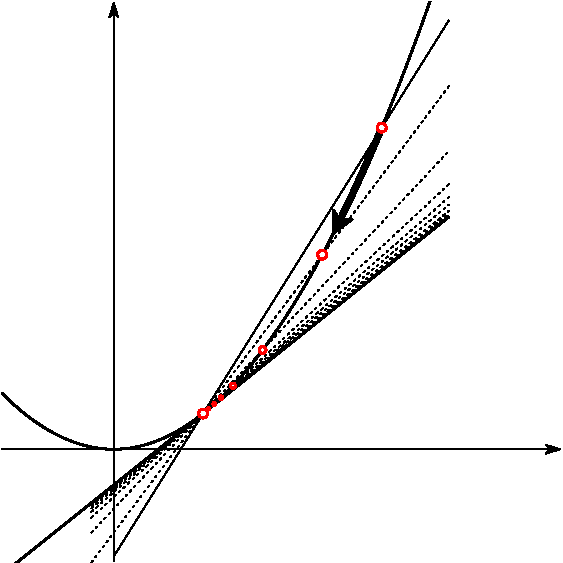
\includegraphics{02constructingTheTangent.pdf}}
        \put( 95.48,  71.75){\sffamily\itshape \makebox[0pt][r]{$P$}}
    \put(181.24, 208.97){\sffamily\itshape \makebox[0pt][r]{$Q$}}
    \put(217.40, 166.09){\sffamily\itshape tangent}
    \put(217.40, 260.42){\sffamily\itshape a secant}
\end{picture}

  \caption{Constructing the tangent by letting $Q\to P$}
  \label{fig:constructTheTangent}
\end{figure}

Let $P$ be the point on the graph at which want to draw the tangent.  If you are
making a real paper and ink drawing you would take a ruler, make sure it goes
through $P$, and then turn it until it doesn't cross the graph anywhere else (at
least, nowhere else near $P$).

If you are using equations to describe the curve and lines, then you
could pick a point $Q$ on the graph and construct the line through $P$
and $Q$ (``construct'' means ``find an equation for'').  This line is
called a ``secant line'', and it won't precisely be the tangent line, but if you
choose $Q$ to be very close to $P$ then the secant line will be close to the
tangent line.

So this is our recipe for constructing the tangent through $P$: pick another
point $Q$ on the graph, find the line through $P$ and $Q$, and see what happens
to this line as you take $Q$ closer and closer to $P$.  The resulting secants
will then get closer and closer to some line, and that line is the tangent.

We'll write this in formulas in a moment, but first let's worry about
how close $Q$ should be to $P$.  We can't set $Q$ equal to $P$,
because then $P$ and $Q$ don't determine a line, since we need \emph{two}
points to determine a line.  If we choose $Q$ different from $P$
then we won't get the tangent, but at best something that is
``close'' to it.  Some people have suggested that one should take $Q$
``infinitely close'' to $P$, but it isn't clear what that would mean.
The concept of a limit is needed to clarify this issue.

\section{An example -- tangent to a parabola} 
\label{sec:tangent-to-parabola}
To make things more concrete, let us take the function $f(x)=x^2$, and attempt
to find the equation of the tangent line to $y=f(x)$ at the point $P=(1, 1)$.
The graph of $f$ is of course a parabola.

Any line through the point $P(1,1)$ has equation
\[
y-1 = m(x-1)
\]
where $m$ is the slope of the line.  So instead of finding the equations of the
secant and tangent lines, we can simply find their slopes.

\begin{center}
  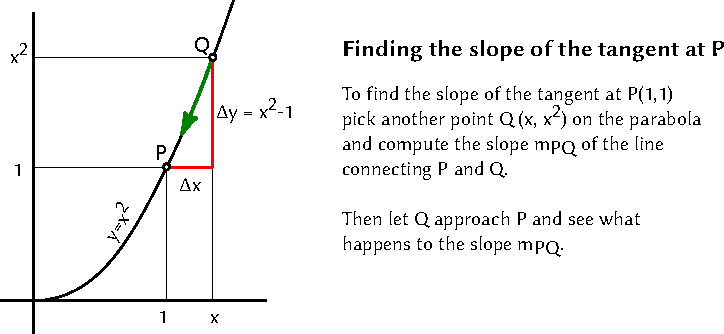
\includegraphics[width=0.7\textwidth]{02DeltaxDeltay.pdf}
\end{center}

Let $Q$ be the other point on the parabola, with coordinates $(x, x^2)$.  We can ``move
$Q$ around on the graph'' by changing $x$, although we are not allowed to set
$x=1$ because $P$ and $Q$ have to be different points.  By the ``rise over run''
formula, the slope of the secant line joining $P$ and $Q$ is
\[
  m_{PQ}= \frac{\Delta y}{\Delta x}
  \quad\text{where}\quad
  \Delta y=x^2-1
  \quad\text{and}\quad
  \Delta x = x-1.
\]
By factoring $x^2-1$ we can rewrite the formula for the slope as follows
\begin{equation}\label{eq:secant-slope-simplified}
  m_{PQ}= \frac{\Delta y}{\Delta x}
  =\frac{x^2-1}{x-1}
  =\frac{(x-1)(x+1)}{x-1}
  = x+1.
\end{equation}
As $x$ gets closer to $1$, the slope $m_{PQ}$, being $x+1$, gets closer to the
value $1+1= 2$.  We say that
\begin{equation*}
  \textit{the limit of the slope $m_{PQ}$ as $Q$ approaches $P$ is $2$.}
\end{equation*}
In symbols,
\[
\lim_{Q\to P} m_{PQ} = 2,
\]
or, since $Q$ approaching $P$ is the same as $x$ approaching 1,
\begin{equation}\label{eq:tangent-slope-found}
  \lim_{x\to 1} m_{PQ} = 2.
\end{equation}
So we find that the tangent line to the parabola $y=x^2$ at the point $(1,1)$ has equation
\[
y-1 = 2 (x-1), \text{~i.e.~} y=2x-1.
\]
A warning: we cannot substitute $x=1$ in equation
\eqref{eq:secant-slope-simplified} to get \eqref{eq:tangent-slope-found}, even
though it looks like that's what we did.  The reason why we can't do that is
that when $x=1$ the point $Q$ coincides with the point $P$ so ``the line through
$P$ and $Q$'' is not defined; also, if $x=1$ then $\Delta x=\Delta y =0$ so that
the rise-over-run formula for the slope gives
\[
m_{PQ} = \frac{\Delta y}{\Delta x} = \frac 00 = \text{~undefined.}
\]
It is only after the algebra trick in \eqref{eq:secant-slope-simplified} that
setting $x=1$ gives something that is well-defined.  But if the intermediate
steps leading to $m_{PQ}=x+1$ aren't valid for $x=1$, why should the final
result mean anything for $x=1$?

We did something more complicated than just setting $x=1$: we did a calculation
which is valid for all $x\neq 1$, and later looked at what happens if $x$ gets
``very close to 1.''  This is the essence of a limit, and we'll study these
ideas in detail soon.


\section{Instantaneous velocity} 
When you are riding in a car, the speedometer tells you how fast you are going,
i.e.\ what your velocity is.  But what exactly does it mean when the speedometer
says your car is traveling at a speed of (say) 50 miles per hour?

\smallskip

\begin{figure}[h]
  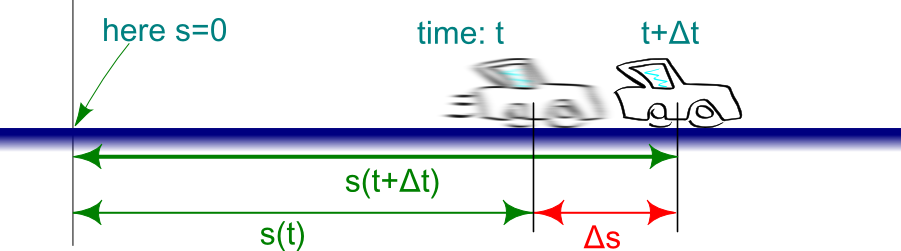
\includegraphics[width=0.6\textwidth]{02car.png}
  %\centering \input ../figures/221/02car.tex
\end{figure}

\smallskip

We all know what \emph{average velocity} is.  Namely, if it takes you two hours
to cover 100 miles, then your average velocity was
\[
\frac{\text{distance traveled}}{\text{time it took}} = 50 \text{ miles per
  hour}.
\]
This is not the number the speedometer provides you -- it doesn't wait two
hours, measure how far you went, and then compute
$\text{distance}/\text{time}$. If the speedometer in your car tells you that you
are driving 50mph, then that should be your velocity \emph{at the moment} that
you look at your speedometer, i.e.\ ``distance traveled over time it took'' at
the moment you look at the speedometer.  But during the moment you look at your
speedometer no time goes by (because a moment has no length) and you didn't
cover any distance, so your velocity at that moment is $\frac00$, which is
undefined.  Your velocity at \emph{any} moment is undefined.  But then what is
the speedometer telling you?

To put all this into formulas we need to introduce some notation.  Let $t$ be
the time (in hours) that has passed since we got onto the road, and let $s(t)$
be our distance from our starting point (in miles).

Instead of trying to find the velocity exactly at time $t$, we find a formula
for the average velocity during some (short) time interval beginning at time
$t$.  We'll write $\Delta t$ for the length of the time interval.

At time $t$ we are $s(t)$ miles from our start.  A little later, at time
$t+\Delta t$ we are $s(t+\Delta t)$ miles from our start.  Therefore, during the
time interval from $t$ to $t+\Delta t$, we have moved
\[
s(t+\Delta t) - s(t)\text{ miles,}
\]
and therefore our average velocity in that time interval was
\[
\frac{s(t+\Delta t) - s(t)}{\Delta t} \text{~ miles per hour.}
\]
The shorter we make the time interval (the smaller we choose $\Delta t$) the
closer this number should be to the instantaneous velocity at time $t$.

So we have the following formula (definition, really) for the velocity at time
$t$
\begin{equation}
  v(t) = \lim_{\Delta t\to0} \frac{s(t+\Delta t)- s(t)}{\Delta t}.
\end{equation}

\section{Rates of change} 
\label{sec:rates-of-change} The two previous examples have much in common.  If
we ignore all the details about geometry, graphs, highways and motion, the
following happened in both examples:

We had a function $y=f(x)$, and we wanted to know how much $f(x)$ changes if $x$
changes.  If we change $x$ to $x+\Delta x$, then $y$ will change from $f(x)$ to
$f(x+\Delta x)$.  The change in $y$ is therefore
\[
\Delta y = f(x+\Delta x) - f(x),
\]
and the average rate of change is
\begin{equation} \label{eq:difference-quotient} \frac{\Delta y}{\Delta x} =
  \frac{f(x+\Delta x) - f(x)}{\Delta x}.
\end{equation}
This is the average rate of change of $f$ over the interval from $x$ to
$x+\Delta x$.  To define \emph{the rate of change of the function $f$ at $x$} we
let the length $\Delta x$ of the interval become smaller and smaller, in the
hope that the average rate of change over the shorter and shorter time intervals
will get closer and closer to some number.  If that happens then that ``limiting
number'' is called the rate of change of $f$ at $x$, or, the \emph{derivative}
of $f$ at $x$.  It is written as
\begin{equation}
  \label{eq:derivative-defined-first-time}
  f'(x) = \lim_{\Delta x\to 0}\frac{f(x+\Delta x) - f(x)}{\Delta x}.
\end{equation}
Derivatives and what we can do with them are what the first portion of this
course is about.  The description we just went through shows that to understand
what a derivative is, we need to understand more about this ``limiting process''
so that we can have a concrete understanding of statements like
\eqref{eq:derivative-defined-first-time}.

\section{Examples of rates of change} 

\subsection{Acceleration as the rate at which velocity changes} 
As you are driving in your car your velocity may change over time.  Suppose
$v(t)$ is your velocity at time $t$ (measured in miles per hour).  You could try
to figure out how fast your velocity is changing by measuring it at one moment
in time (you get $v(t)$), then measuring it a little later (you get $v(t+\Delta
t)$)).  You conclude that your velocity increased by $\Delta v = v(t+ \Delta t)
- v(t)$ during a time interval of length $\Delta t$, and hence
\begin{multline*}
  \left\{
    \parbox{7em}{\centering average rate at which your velocity changed}
  \right\}
  = \frac{\text{change in velocity}}{\text{duration of time interval}}
  =\frac{\Delta v}{\Delta t} =\frac{v(t+ \Delta t) - v(t)}{\Delta t}.
\end{multline*}
This rate of change is called your \textit{average acceleration} (over the time
interval from $t$ to $t+\Delta t$).  Your \textit{instantaneous acceleration} at
time $t$ is the limit of your average acceleration as you make the time interval
shorter and shorter:
\[
\left\{ \text{acceleration at time $t$} \right\} = a = \lim_{\Delta t\to 0}
\frac{v(t+ \Delta t) - v(t)}{\Delta t}.
\]
The average and instantaneous accelerations are measured in ``miles per hour per
hour'':
\[
(\textrm{mi}/\textrm{h})/\textrm{h} = \textrm{mi}/\textrm{h}^2.
\]
Or, if you had measured distances in \textit{meters} and time in
\textit{seconds} then velocities would be measured in \textit{meters per
  second}, and acceleration in \textit{meters per second per second}, which is
the same as meters per second$^2$: ``meters per squared second''.




\subsection{Reaction rates} 
Imagine a chemical reaction in which two substances A and B react in such a way
that A converts B into A.  The reaction could proceed by
\[
\textrm{A} +  \textrm{B} \longrightarrow 2\textrm{A}.
\]
If the reaction is taking place in a closed reactor, then the ``amounts'' of A
and B will change with time.  The amount of B will decrease, while the amount of
A will increase.  Chemists write $[\textrm{A}]$ for the concentration of ``A''
in the chemical reactor (measured in moles per liter).  We're mathematicians so
we will write ``$[\textrm{A}](t)$'' for the concentration of A present at time
$t$.
\begin{figure}[h]
  \begin{center}
    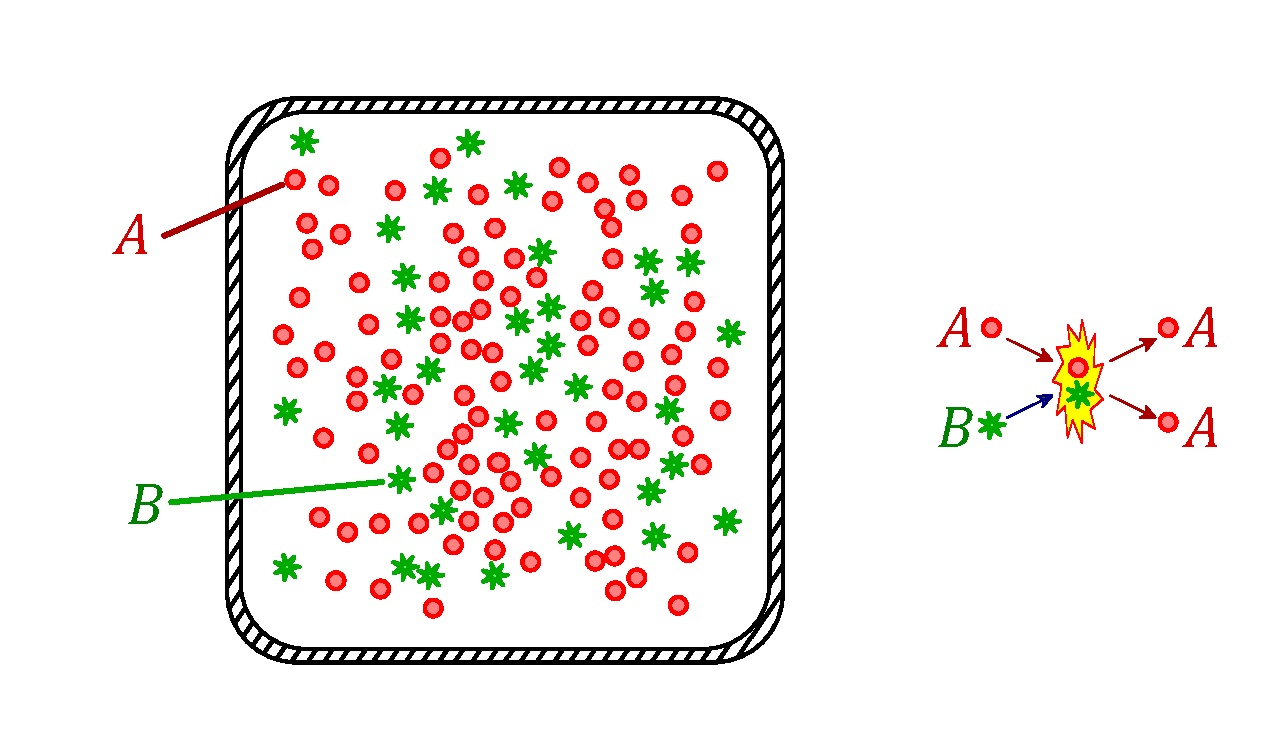
\includegraphics[width=0.6\textwidth]{02ABreaction.pdf}
  \end{center}
  \caption{A chemical reaction in which A converts B into A.}
  \label{fig:02ABreaction}
\end{figure}

To describe how fast the amount of A is changing we consider the derivative
of $[\textrm{A}]$ with respect to time:
\[
[A]'(t)= \lim_{\Delta t\to 0}
\frac {[\textrm{A}](t+\Delta t) - [\textrm{A}](t)}  {\Delta t}.
\]
This quantity is the rate of change of [A].  In chemistry and physics, it is
more common to write the derivative in \textsc{Leibniz} notation:
\[
\frac{d[\textrm{A}]}{dt}.
\]

\textit{How fast does the reaction take place?}  If you add more A or more B to
the reactor then you would expect that the reaction would go faster (i.e., that
more A would be produced per second).  The law of \textit{mass-action kinetics}
from chemistry states this more precisely. For our particular reaction it would
say that the rate at which A is consumed is given by
\[
\frac{d[\textrm{A}]}{dt} = k \, [\textrm{A}] \, [\textrm{B}],
\]
where the constant $k$ is called the \textit{reaction constant}, which you could
measure by timing how fast the reaction goes.

\section{Problems} 
\problemfont% 
\begin{multicols}{2}\setlength{\parindent}{0pt}
\problem \label{ex:02derivATonethird} 
Repeat the reasoning in \S\ref{sec:tangent-to-parabola} to find the slope of the
tangent line at the point $(\frac13, \frac19)$, or more generally at any point
$(a, a^2)$ on the parabola with equation $y=x^2$.

\problem Repeat the reasoning in \S\ref{sec:tangent-to-parabola} to find the 
slope of the tangent line at the point $(\frac12, \frac18)$, or more generally
at any point $(a, a^3)$ on the curve with equation $y=x^3$.

\problem Simplify the algebraic expressions you get when you compute $\Delta y$ and 
$\Delta y/\Delta x$ for the following functions
\begin{align*}
  (a)~& y = x^2-2x+1 \\
  (b)~& y = \frac1x \\
  (c)~& y = 2^x
  \end{align*}
\answer 
\textbf{(a)}
\begin{align*}
  \Delta y &= (x+\Delta x)^2  -2 (x+\Delta x)+1 - [x^2-2x+1]\\
  &=(2x-2)\Delta x +(\Delta x)^2 \text{ so that}\\
  \frac{\Delta y}{\Delta x}&= 2x-2 + \Delta x
\end{align*}
\endanswer

\problem This figure shows a plot of the distance traveled $s(t)$ (in miles)
versus time $t$ (in minutes):
\smallskip

\centerline{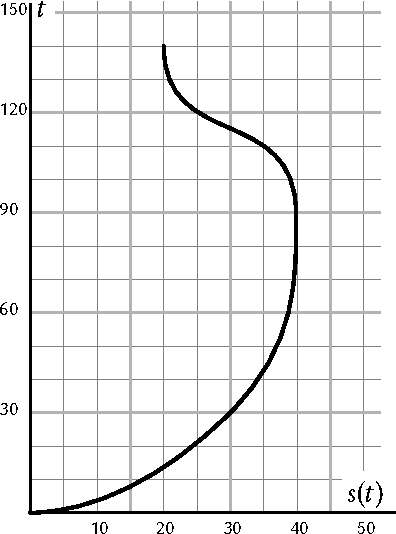
\includegraphics[width=0.4\textwidth]{02velocityproblem.pdf}}

\subprob Something is wrong:  the curve in the graph obviously doesn't pass the vertical
line test, so it cannot be the graph of a function.  How can it be the graph of $s(t)$
versus $t$?
% This problem statement is incredibly misleading ("graph of a function").
\answer 
In this picture $s(t)$ is on the horizontal axis and $t$ is on the vertical axis, so
horizontal and vertical have been swapped. This curve should pass the \emph{horizontal
line test}, which it does.
\endanswer

\subprob Use the plot to estimate the instantaneous
velocity at the following times
\begin{center}
  \begin{tabular}{cp{1in}}
    \toprule
    $t$ (min) &\hfill $v(t)$ \\[1pt]
    \midrule
    30 & \\[1pt]
    \midrule
    60 & \\[1pt]
    \midrule
    90 & \\[1pt]
    \midrule
    120 & \\
    \bottomrule
  \end{tabular}
\end{center}
Describe in one or two short sentences what you did to find
your estimates.
\answer 
With a ruler I tried to draw the closest tangent lines at
the four different times.  Then I measured the slope of those
four lines using the grid.
\endanswer

\subprob Make a graph of the instantaneous velocity $v(t)$.

\problem Look ahead at Figure~\ref{fig:03backwardCosSandwich} in the next 
chapter.  What is the derivative of $f(x) = x\cos\frac\pi x$ at the
points $A$ and $B$ on the graph?
\answer 
At $A$ and $B$ the graph of $f$ is tangent to the drawn lines, so
the derivative at $A$ is $-1$ and ther derivative at $B$ is $+1$.
\endanswer
  
\problem Suppose that some quantity $y$ is a function of some other quantity 
$x$, and suppose that $y$ is a mass (measured in pounds)
and $x$ is a length (measured in feet).  What units do the increments
$\Delta y$ and $\Delta x$, and the derivative $ dy/d x$, have?
\answer 
$\Delta x$ : feet.  $\Delta y$ pounds. $\frac{\Delta y}{\Delta x}$
and $\frac{dy}{dx}$ are measured in pounds per feet.
\endanswer

\problem A tank is filling with water.  The volume (in gallons) of water in 
the tank at time $t$ (seconds) is $V(t)$.  What units does the
derivative $V'(t)$ have?
\answer 
Gallons per second.
\endanswer

\problem \groupproblem Let $A(x)$ be the area of an equilateral triangle whose
sides measure $x$ inches.
% This problem is not appropriate for this chapter, where derivatives have not
% even been defined.

\subprob Show that $\frac{dA}{dx}$ has the units of a length.

\subprob Which length does $\frac{dA}{dx}$ represent geometrically?  [Hint: draw
two equilateral triangles, one with side $x$ and another with side $x+\Delta x$.
Arrange the triangles so that they both have the origin as their lower left hand
corner, and so their bases are on the x-axis.]

\answer 
(a) $A(x)$ is an area so it has units square inch and $x$ is
measured in inches, so $\dfrac{dA}{dx}$ is measured in
$\displaystyle\frac{\text{inch}^2}{\text{inch}} = \text{inch}$.

\input ../figures/221/02triangleareagrowth.tex

(b) Hint: The extra area $\Delta A$ that you get when the side of
an equilateral triangle grows from $x$ to $x+\Delta x$ can be
split into a thin parallelogram and a very tiny triangle.  Ignore
the area of the tiny triangle since the area of the parallelogram
will be much larger.  What is the area of this parallelogram?




The area of a parallelogram is ``base time height'' so here it is
$h\times\Delta x$, where $h$ is the height of the triangle.




Conclusion: $\displaystyle \frac{\Delta A}{\Delta x}
\approx\frac{h\Delta x}{\Delta x} = h$.




The derivative is therefore the height of the triangle.




\endanswer








\problem \groupproblem Let $A(x)$ be the area of a square with 
side $x$, and let $L(x)$ be
the perimeter of the square (sum of the lengths of all its sides).
Using the familiar formulas for $A(x)$ and $L(x)$ show that $A'(x) =
\frac12 L(x)$.
% This problem is not appropriate for this chapter, where derivatives have not even been defined.


Give a geometric interpretation that explains why $\Delta A \approx
\frac12 L(x) \Delta x$ for small $\Delta x$.








\problem Let $A(r)$ be the area enclosed by a circle of radius $r$, and let 
$L(r)$ be the circumference of the circle.  Show that $ A'(r) = L(r) $.
(Use the familiar formulas from geometry for the area and circumference
of a circle.)
% This problem is not appropriate for this chapter, where derivatives have not even been defined.






\problem Let $V(r)$ be the volume enclosed by a sphere of radius $r$, and let 
$S(r)$ be the its surface area.
% This problem is not appropriate for this chapter, where derivatives have not even been defined.


\subprob Show that $V'(r) = S(r)$.  (Use the
formulas $V(r) = \frac43\pi r^3$ and $S(r) = 4\pi r^2$.)




\subprob Give a geometric explanation of the fact that
$\frac{dV} {dr} = S$.




[Hint: to visualize what happens to the volume of a sphere when
you increase the radius by a very small amount, imagine  the sphere is
the Earth, and you increase the radius by covering the Earth with
a layer of water that is 1 inch deep.  How much does the volume
increase?  What if the depth of the layer was ``$\Delta r$''?]




\problem \label{ex:bad-calculator-bad} \groupproblem 
\itshape Should you trust your calculator?\upshape




Find the slope of the tangent to the parabola
\[
y=x^2
\]
at the point
$(\frac13, \frac{1}{9})$ (You have already done this: see exercise
\ref{ex:02derivATonethird}).




Instead of doing the algebra you could try to compute the slope by
using a calculator.  This exercise is about how you do that and what
happens if you try (too hard).




Compute $\frac{\Delta y}{\Delta x}$ for various values of $\Delta x$:
\[
\Delta x = 0.1, 0.01, 0.001, 10^{-6}, 10^{-12}.
\]
As you choose $\Delta x$ smaller your computed $\frac{\Delta
  y}{\Delta x}$ ought to get closer to the actual slope.  Use at
least 10 decimals and organize your results in a table like this:
Look carefully at the ratios $\Delta y/\Delta x$.  Do they look like
they are converging to some number?  Compare the values of
$\frac{\Delta y}{\Delta x}$ with the true value you got in the
beginning of this problem.












\end{multicols}
\noproblemfont




\begin{table}[h]
  \centering
  \begin{tabular}{r|p{75pt}|p{75pt}|p{75pt}|p{75pt}}
    \hline\rule[-6pt]{0pt}{18pt}
    $\Delta x$ & $a+\Delta x$ & $f(a+\Delta x)$ & $\Delta y$ & $\Delta y / \Delta x$ \\
    \hline\rule[-6pt]{0pt}{18pt}
    \texttt{0.1} &&&&\\
    \hline\rule[-6pt]{0pt}{18pt}
    \texttt{0.01} &&&&\\
    \hline\rule[-6pt]{0pt}{18pt}
    \texttt{0.001} &&&&\\
    \hline\rule[-6pt]{0pt}{18pt}
    \texttt{10}$^{\texttt{-6}}$ &&&&\\
    \hline\rule[-6pt]{0pt}{18pt}
    \texttt{10}$^{\texttt{-12}}$ &&&&\\
    \hline
  \end{tabular}
  \medskip
  
  \caption{The table for Problem~\ref{ex:bad-calculator-bad}.
  Approximate the derivative of $f(x) = x^2$ at
  $a=1/3 \approx 0.333\,333\,333\,333$ by computing $\bigl(f(a+\Delta
  x) - f(a)\bigr)/\Delta x$ for smaller and smaller values of $\Delta
  x$.  You know from Problem~\ref{ex:02derivATonethird} that
  the derivative is $f'(a) = 2a = 2/3$.  Which value of
  $\Delta x$ above gives you the most accurate answer?}
\end{table}


%%% Local Variables:
%%% mode: latex
%%% TeX-master: "free221"
%%% End:

% !TEX root =  free221.tex

\chapter{Limits and Continuous Functions}
While it is easy to define precisely in a few words what a square root
is ($\sqrt{a}$ is the positive number whose square is $a$) the
definition of the limit of a function is more complicated.  In this
chapter we will take three approaches to defining the limit.
The first definition (\S\ref{sec:informal-limit-def}) appeals to
intuition and puts in words how most people think about limits.
Unfortunately this definition contains language that is ambiguous and
the more you think about it the more you realize that it actually
doesn't mean anything.  It is also not clear enough to answer all questions that
come up about limits.

Most of the calculus you'll see in this semester was essentially invented
in the 17th century, but the absence of a good definition of what
derivatives and limits are led to centuries of confused arguments between
experts.  These more or less ended when a precise definition was developed
in the late 19th century, 200 years after calculus was born!  In
\S\ref{sec:formal-limit-def} you'll see this precise definition.  It runs
over several terse lines, and unfortunately most people don't find it very
enlightening when they first see it.
The third approach we will take is the \emph{axiomatic approach}:
instead of worrying about the details of what a limit is, we use our
intuition and in \S\ref{sec:limitProperties} we write down a number of
properties that we believe the limit should have.  After that we try
to base all our reasoning on those properties.

\section{Informal definition of limits} 
\label{sec:informal-limit-def}

\subsection{Definition of limit (1st attempt)} 
\itshape\label{def:limit-first-attempt}
If $f$ is some function then
\[
\lim_{x\to a} f(x) = L
\]
is read ``the limit of $f(x)$ as $x$ approaches $a$ is $L$.''  It
means that if you choose values of $x$ that are close \emph{but not
  equal} to $a$, then $f(x)$ will be close to the value $L$; moreover,
$f(x)$ gets closer and closer to $L$ as $x$ gets closer and closer to
$a$.  \upshape\smallskip

The following alternative notation is sometimes used
\[
f(x)\to L \quad\text{ as } \quad x\to a;
\]
(read ``$f(x)$ approaches $L$ as $x$ approaches $a$'' or ``$f(x)$ goes to
$L$ as $x$ goes to $a$''.)

Note that in the definition we require $x$ to approach $a$ without
ever becoming equal to $a$.  It's important that $x$ never actually
equals $a$ because our main motivation for looking at limits was
the definition of the derivative.  In Chapter II, equation
\eqref{eq:derivative-defined-first-time} we defined the derivative of
a function as a limit in which some number $\Delta x$ goes to zero:
\[
f'(x) = \lim_{\Delta x\to0} \frac{f(x+\Delta x)-f(x)}{\Delta x}.
\]
The quantity whose limit we want to take here is not even defined when
$\Delta x=0$.  Therefore any definition of limit we come up with had
better not depend on what happens at $\Delta x=0$; likewise, the limit
$\lim_{x\to a}f(x)$ should not depend on what $f(x)$ does at $x=a$.
\subsection{Example} 
If $f(x) = x+3$ then
\[
\lim_{x\to 4} f(x) = 7,
\]
is ``true'', because if you substitute numbers $x$ close to $4$ in $f(x) = x+3$
the result will be close to $7$.
\subsection{A complaint} 
Our first definition relies heavily on the
phrase ``gets close to'' or ``gets closer and closer to''.  What does
this mean?  When $x$ gets closer and closer to $a$ without ever being
equal to $a$, how long does this take? (``are we there yet?'') How
close is close enough?  Is it enough for $x$ and $a$ to be the same in
five decimals?  Fifty decimals?  It is hard to answer these questions without
generating new ones.

If we want to deal with limits with some measure of confidence that what we are
doing isn't ultimately nonsense, then we will need a better definition of limit.
Before going into that, let's look at a practical approach to finding limits.
To compute $\lim_{x\to a} f(x)$ we need to let $x$ get closer and closer to $a$;
we don't really know how to do that, but we can certainly grab a calculator or a
computer and compute $f(x)$ for several values of $x$ that are somewhat close to
$a$ ($a$ to two decimals, $a$ to three decimals, etc.)  If the values of $f(x)$
then begin to look like some fixed number we could guess that that number is the
limit \footnote{This idea of making better and better approximations is actually
a common approach in modern science: if you have a complicated problem (such as
predicting tomorrow's weather, or the next three decades' climate) that you
cannot solve directly, one thing often tried is changing the problem a little
bit, and then making approximations with a computer.  This activity is called
\emph{Scientific Computation}, a very active branch of modern mathematics.}.  

Here are two examples where we try to find a limit by calculating
$f(x)$ for a few values of $x$:

\subsection{Example: substituting numbers to guess a limit} 
\label{ex:limit-by-sub-good}
What (if anything) is
\[
\lim_{x\to 2}\frac{x^2 -2x}{x^2-4}?
\]
Here $f(x) = (x^2 - 2x)/(x^2-4)$ and $a=2$.


We first try to substitute $x=2$, but this leads to
\[
f(2) = \frac{2^2 - 2\cdot2}{2^2-4} = \frac 00
\]
which does not exist.  Next we try to substitute values of $x$ close but
not equal to $2$.  Table \ref{tbl:finding-limits} suggests that $f(x)$
approaches $0.5$.


\begin{table}[ht]
  \centering
  \begin{tabular}{ll}
    \toprule
    \quad$x$ & \quad$f(x)$ \\
    \midrule
    3.000000 & 0.600000\\
    2.500000 & 0.555556\\
    2.100000 & 0.512195\\
    2.010000 & 0.501247\\
    2.001000 & 0.500125\\
    $\downarrow$& \hfil$\downarrow$\hfil\\
    2 & \hfil limit?\hfil\\
    \bottomrule
  \end{tabular}
  \qquad\qquad
  \begin{tabular}{ll}
    \toprule
    \quad$x$ & \quad$g(x)$ \\
    \midrule
    1.000000 & 1.009990\\
    0.500000 & 1.009980\\
    0.100000 & 1.009899\\
    0.010000 & 1.008991\\
    0.001000 & 1.000000\\
    $\downarrow$& \hfil$\downarrow$\hfil\\
    0& \hfil limit?\hfil\\
    \bottomrule
  \end{tabular}
  \smallskip
% !!! Issue: should this table split into 2 tables to fill in the missing data for limits from below? (and to separate f and g from each other)
  
  \caption{Finding limits by substituting values of $x$ ``close to $a$.''
    (Values of $f(x)$ and $g(x)$ rounded to six decimals.)}
  \label{tbl:finding-limits}
\end{table}  

\subsection{Example: substituting numbers can suggest the wrong answer} 
\label{ex:limit-by-sub-bad}
Suppose we had the function
\[
g(x) = \frac{101\,000x}{100\,000x+1}
\]
and we want to find the limit $\lim_{x\to0}g(x)$.

Then substitution of some ``small values of $x$'' could lead us to believe
that the limit is $1.000\ldots$.  But in fact, if we substitute sufficiently
small values, we will see that the limit is $0$ (zero)!
As you see from this example, there's more to evaluating limits
than just typing numbers into the computer and hitting return.  See
also problem \ref{ex:bad-calculator-bad}.
\section{Problems} 
\problemfont 
\begin{multicols}{2}
\problem Guess $\lim_{x\to 2} x^{10}$. 
Then try using the first definition of the limit to show that your
guess is right.
\problem Use a calculator to guess the value of 
\[
\lim_{x\to0} \bigl(1+x\bigr)^{1/x}.
\]

\problem Is the limit 
$\lim_{x\to0} (1+0.693x)^{1/x}$
an integer?  Give reasons for your answer, and compare with your
neighbor's answer.

\problem Simplicio computed $2^{-10} \approx 0.001$ which is very 
close to zero.  He therefore concludes that if $x$ is very close to
$2$, then $x^{-10}$ is very close to zero, so that, according to
Simplicio, it is clearly true that
\[
\lim_{x\to2} x^{-10} = 0.
\]
Comment on Simplicio's reasoning: do you agree with his answer?  Do
you agree with his reasoning?

\problem Use a calculator to guess\\[6pt] 

\subprob $\DS\lim_{x\to1} \frac{x^{100}}{1.01+x^{100}}$.\\[6pt]

\subprob $\DS\lim_{x\to1} \frac{1.01-x^{100}}{x^{100}}$.\\[6pt]

\subprob $\DS\lim_{x\to1} \frac{x^{100}}{1.01-x^{100}}$.

\end{multicols}
\noproblemfont

\section{The formal, authoritative, definition of limit} 
\label{sec:formal-limit-def} Our attempted definitions of the limit
uses undefined and non-mathematical phrases like ``closer and closer''.
In the end we don't really know what those statements really mean, although they are
suggestive.  Fortunately, there is a good definition, one
that is unambiguous and can be used to settle any dispute about the
question of whether $\lim_{x\to a} f(x)$ equals some number $L$ or
not.  Here is the definition.  

\subsection{Definition of $\lim_{x\to a} f(x) = L$} 
\itshape%
If $f(x)$ is a function defined for all $x$ in some interval which contains $a$,
except possibly at $x=a$, then we say that $L$ is the limit of $f(x)$ as $x\to
a$, if for every $\varepsilon>0$, we can find a $\delta>0$ (depending on
$\epsilon$) such that for all $x$ in the domain of $f$ it is true that
\begin{equation}\label{eq:03limitdef}
    0 < |x-a| < \delta \text{ implies } |f(x) - L|<\varepsilon.
\end{equation}
\upshape

\subsection*{Why the absolute values? } 
The quantity $|x-y|$ is the distance between the points $x$ and $y$ on
the number line, and one can measure how close $x$ is to $y$ by
calculating $|x-y|$.  The inequality $|x-y|<\delta$ says that ``the
distance between $x$ and $y$ is less than $\delta$,'' or that ``$x$
and $y$ are closer than $\delta$.''

\subsection*{What are $\varepsilon$ and $\delta$?} 
The quantity $\varepsilon$ is how close you would like $f(x)$ to be to
its limit $L$; the quantity $\delta$ is how close you have to choose
$x$ to $a$ to achieve this.  To prove that $\lim_{x\to a} f(x) = L$
you must assume that someone has given you an unknown $\varepsilon>0$,
and then find a positive $\delta$ for which \eqref{eq:03limitdef}
holds.  The $\delta$ you find will depend on $\varepsilon$.


\begin{figure}
  
    \begin{picture} (180.000000,180.000000)(0,0)
    \put(0.0, 0.0){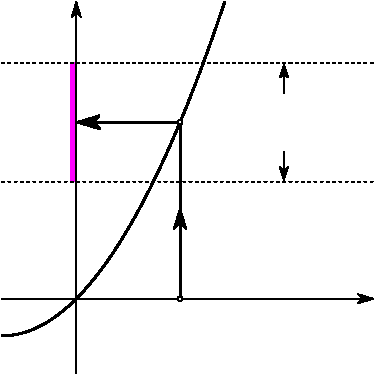
\includegraphics{03epsAndNoDelta.pdf}}
        \put( -2.00,  92.85){\sffamily\itshape \makebox[0pt][r]{$L-\varepsilon$}}
    \put( -2.00, 149.81){\sffamily\itshape \makebox[0pt][r]{$L+\varepsilon$}}
    \put( 31.60, 121.33){\sffamily\itshape \makebox[0pt][r]{$L$}}
    \put(108.24, 168.50){\sffamily\itshape $y=f(x)$}
    \put( 84.44,  24.60){\sffamily\itshape $a$}
    \put( 91.44, 121.33){\sffamily\itshape \
How close must $x$ be to $a$ for $f(x)$ to end up in this range?
}
\end{picture}


  
    \begin{picture} (180.000000,180.000000)(0,0)
    \put(0.0, 0.0){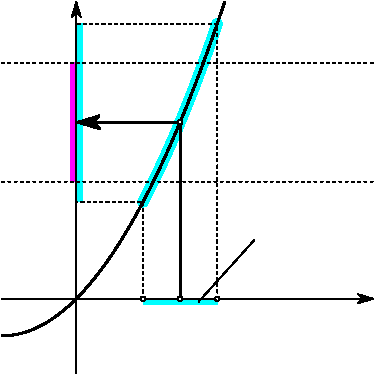
\includegraphics{03epsAndDeltaTooBig.pdf}}
        \put( -2.00,  92.85){\sffamily\itshape \makebox[0pt][r]{$L-\varepsilon$}}
    \put( -2.00, 149.81){\sffamily\itshape \makebox[0pt][r]{$L+\varepsilon$}}
    \put( 31.60, 121.33){\sffamily\itshape \makebox[0pt][r]{$L$}}
    \put(108.24, 168.50){\sffamily\itshape $y=f(x)$}
    \put(107.24,  39.60){\sffamily\itshape $a+\delta$}
    \put( 44.64,  39.60){\sffamily\itshape $a-\delta$}
    \put( 84.44,  24.60){\sffamily\itshape $a$}
    \put(125.04,  64.72){\sffamily\itshape \begin{minipage}{240pt}
        For some $x$ in this interval $f(x)$ is not between
        $L-\varepsilon$ and $L+\varepsilon$. Therefore the $\delta$ in this
        picture is too big for the given $\varepsilon$.  You need a smaller
        $\delta$.
        \end{minipage}}
\end{picture}


  
    \begin{picture} (180.000000,180.000000)(0,0)
    \put(0.0, 0.0){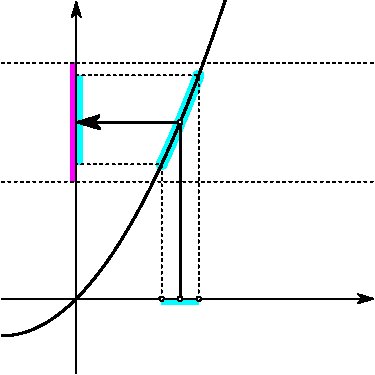
\includegraphics{03epsAndDelta.pdf}}
        \put( -2.00,  92.85){\sffamily\itshape \makebox[0pt][r]{$L-\varepsilon$}}
    \put( -2.00, 149.81){\sffamily\itshape \makebox[0pt][r]{$L+\varepsilon$}}
    \put( 31.60, 121.33){\sffamily\itshape \makebox[0pt][r]{$L$}}
    \put(108.24, 168.50){\sffamily\itshape $y=f(x)$}
    \put( 98.34,  39.60){\sffamily\itshape $a+\delta$}
    \put( 53.54,  39.60){\sffamily\itshape $a-\delta$}
    \put( 84.44,  24.60){\sffamily\itshape $a$}
\end{picture}

\end{figure}

\begin{figure}[t]
  \framebox{
    \begin{minipage}{0.95\textwidth} \sffamily \null \smallskip

      \centerline{\bfseries Propagation of errors -- another interpretation
        of $\varepsilon$ and $\delta$} \vbox to2pt{} According to the limit
      definition ``$\lim_{x\to R} \pi x^2 = A$'' is true if \textit{for
        every $\varepsilon>0$ you can find a $\delta>0$ such that $|x-R| <
        \delta$ implies $|\pi x^2 - A| < \varepsilon$.  } Here's a more
      concrete situation in which $\varepsilon$ and $\delta$ appear in
      exactly the same roles:

      \vbox to 2pt{}

      \begin{multicols}{2}\setlength{\parindent}{0pt}
      \setlength{\parindent}{2em}
      \noindent
      Suppose you are given a circle drawn on a piece of paper, and you
      want to know its area.  You decide to measure its radius, $R$,
      and then compute the area of the circle by calculating
      \[
      \textsf{Area} = \pi R^2.
      \]
      The area is a function of the radius, and we'll call that
      function $f$:
      \[
      f(x) = \pi x^2.
      \]

      When you measure the radius $R$ you will make an error, simply
      because you can never measure anything with infinite accuracy.
      Suppose that $R$ is the real value of the radius, and that $x$ is
      the number you measured.  Then the size of the error you made is
      \[
      \textsf{error in radius measurement} = |x-R|.
      \]
      When you compute the area you also won't get the exact value: you
      would get $f(x) = \pi x^2$ instead of $A = f(R) = \pi R^2$.  The
      error in your computed value of the area is
      \[
      \textsf{error in area } = |f(x) - f(R)| = |f(x) - A|.
      \]
      Now you can ask the following question:
      \begin{center}
        \itshape
        Suppose you want to know the area\\
        with an error of at most $\varepsilon$,\\
        then what is the largest error\\
        that you can afford to make\\
        when you measure the radius?
      \end{center}
      The answer will be something like this: if you want the computed
      area to have an error of at most $|f(x) - A| < \varepsilon$, then
      the error in your radius measurement should satisfy $|x-R| <
      \delta$.  You have to do the algebra with inequalities to compute
      $\delta$ when you know $\varepsilon$, as in the examples in this
      section.

      You would expect that if your measured radius $x$ is close enough
      to the real value $R$, then your computed area $f(x) = \pi x^2$
      will be close to the real area $A$.

      In terms of $\varepsilon$ and $\delta$ this means that you would
      expect that no matter how accurately you want to know the area
      (i.e., how small you make $\varepsilon$) you can always achieve
      that precision by making the error in your radius measurement
      small enough (i.e.  by making $\delta$ sufficiently small).
    \end{multicols}
    \vbox to2pt{}
  \end{minipage} }
\end{figure}

\subsection{Show that $\lim_{x\to 5}(2x+1)=11$ . } 
We have $f(x) = 2x+1$, $a=5$ and $L=11$, and the question we must answer is
``how close should $x$ be to $5$ if want to be sure that $f(x)=2x+1$
differs less than $\varepsilon$ from $L=11$?''

To figure this out we try to get an idea of how big $|f(x)-L|$ is:
\[
|f(x)-L| = \bigl|(2x+1)-11\bigr| = |2x-10| = 2\cdot |x-5| = 2\cdot |x-a|.
\]
So, if $2|x-a|<\varepsilon$ then we have $|f(x)-L|<\varepsilon$, i.e.,
\[
\text{if }|x-a|<\tfrac12\varepsilon \text{ then } |f(x)-L|<\varepsilon.
\]
We can therefore choose $\delta = \frac12\varepsilon$.  No matter what
$\varepsilon>0$ we are given our $\delta$ will also be positive, and if
$|x-5|<\delta$ then we can guarantee $|(2x+1) - 11|<\varepsilon$.  That
shows that $\lim_{x\to 5}2x+1 = 11$.




\subsection{The limit $\lim_{x\to 1}x^2 = 1$, the triangle inequality, and the ``don't choose $\delta>1$'' trick} 
This example will show you two basic tricks that are useful in many
$\varepsilon$-$\delta$ arguments.

The problem is to show that $x^2$ goes to 1 as $x$ goes to 1: we have $f(x) =
x^2$, $a=1$, $L=1$, and again the question is, ``how small should $|x-1|$ be to
guarantee $|x^2-1|<\varepsilon$?''

We begin by estimating the difference $|x^2-1|$
\[
|x^2-1| = |(x-1)(x+1)| = |x-1|\cdot|x+1|.
\]
How big can the two factors $|x-1|$ and $|x+1|$ be when we assume
$|x-1|<\delta$?  Clearly the first factor $|x-1|$ satisfies $|x-1|<\delta$
because that is what we had assumed.
\marginpar{\footnotesize\sffamily%
  The triangle inequality says that\\
  $|a+b|\leq |a| + |b|$\\
  for any two real numbers.}%
For the second factor we have
\[
|x+1| = \underbrace{|x-1 +2| \leq |x-1| + |2|}_{\text{by the triangle inequality}}
\leq \delta + 2.
\]
It follows that if $|x-1|<\delta$ then
\[
|x^2-1| \leq (2+\delta)\delta.
\]
Our goal is to show that if $\delta$ is small enough then the estimate on the
right will not be more than $\varepsilon$.  Here is the second trick in this
example: we agree \textit{that we always choose our $\delta$ so that $\delta\leq
1$.}  If we do that, then we will always have
\[
(2+\delta)\delta < (2+1)\delta =3\delta,
\]
so that $|x-1|<\delta$ with $\delta<1$ implies
\[
|x^2-1| < 3\delta.
\]
To ensure that $|x^2-1|<\varepsilon$, this calculation shows that we should
require $3\delta\leq \varepsilon$, i.e.\ we should choose $\delta \leq
\frac13\varepsilon$.  We must also live up to our promise never to choose
$\delta>1$, so if we are handed an $\varepsilon$ for which
$\frac13\varepsilon>1$, then we choose $\delta=1$ instead of $\delta =
\frac13\varepsilon$.  To summarize, we are going to choose
\[
\delta = \text{the smaller of }1\text{ and }\frac13\varepsilon.
\]
We have shown that for $\delta$ defined this way, then $|x-1|<\delta$
implies $|x^2-1|<\varepsilon$, no matter what $\varepsilon>0$ is.

The expression ``the smaller of $a$ and $b$'' shows up often, and is
abbreviated to $\min(a, b)$.  We could therefore say that in this problem
we will choose $\delta$ to be
\[
\delta = \min \bigl(1, \tfrac13 \varepsilon\bigr).
\]


\subsection{Show that $\lim_{x\to 4}1/x = 1/4$} 

We apply the definition with $a=4$, $L=1/4$ and $f(x) = 1/x$.
Thus, for any $\varepsilon>0$ we try to show that if $|x-4|$ is small
enough then one has $|f(x)-1/4|<\varepsilon$.

We begin by estimating $|f(x)-\frac14|$ in terms of $|x-4|$:
\[
|f(x)-1/4| = \left|\frac1x-\frac14\right| = \left| \frac{4-x}{4x}\right| =
\frac{|x-4|}{|4x|} =\frac{1}{|4x|}\,|x-4|.
\]
As before, things would be easier if $1/|4x|$ were a constant.  To achieve that
we again agree not to take $\delta>1$.  If we always have $\delta\leq 1$, then
we will always have $|x-4|<1$, and hence $3<x<5$.  How large can $1/|4x|$ be in
this situation?  Answer: the quantity $1/|4x|$ increases as you decrease $x$, so
if $3<x<5$ then it will never be larger than $1/|4\cdot 3| = \frac1{12}$.
We see that if we never choose $\delta>1$, we will always have
\[
|f(x) - \tfrac14|\leq \tfrac1{12}|x-4| \quad\text{for}\quad |x-4|<\delta.
\]
To guarantee that $|f(x)-\frac14|<\varepsilon$ we could therefore require
\[
\tfrac1{12} |x-4|<\varepsilon, \quad\text{i.e.}\quad |x-4| <12\varepsilon.
\]
Hence if we choose $\delta=12\varepsilon$ or any smaller number, then
$|x-4|<\delta$ implies $|f(x)-4|<\varepsilon$.  Of course we have to honor
our agreement never to choose $\delta>1$, so our choice of $\delta$ is
\[
\delta = \text{the smaller of }1\text{ and }12\varepsilon = \min \bigl(1,
12\varepsilon\bigr).
\]

\section{Problems} 
\problemfont 
\problem \groupproblem Joe offers to make square sheets of paper for 
Bruce.  Given $x>0$ Joe plans to mark off a length $x$ and cut out a
square of side $x$.  Bruce asks Joe for a square with area 4 square
foot.  Joe tells Bruce that he can't measure \emph{exactly} 2 feet and
the area of the square he produces will only be approximately 4 square
feet.  Bruce doesn't mind as long as the area of the square doesn't
differ more than $0.01$ square feet from what he really asked for
(namely, 4 square foot).

\subprob What is the biggest error Joe can afford to make when he
marks off the length $x$?

\subprob Jen also wants square sheets, with area $4$ square feet.
However, she needs the error in the area to be less than $0.00001$
square foot.  (She's paying.)

How accurately must Joe measure the side of the squares he's going to cut
for Jen?

\problem \groupproblem \textit{(Joe goes cubic.)}  Joe is offering to 
build cubes of side $x$.  Airline regulations allow you take a cube on
board provided its volume and surface area add up to less than $33$
(everything measured in feet).  For instance, a cube with 2-foot sides
has volume$+$area equal to $2^3 + 6\times 2^2 = 32$.

If you ask Joe to build a cube whose volume plus total surface area is
$32$ with an error of at most $\varepsilon$, then what error
can he afford to make when he measures the side of the cube he's
making?

\problem Our definition of a derivative in 
\eqref{eq:derivative-defined-first-time} contains a limit.  What is the
function ``$f$'' there, and what is the variable?
\answer 
The equation \eqref{eq:derivative-defined-first-time} already
contains a function $f$, but that is not the right function.  In
\eqref{eq:derivative-defined-first-time} $\Delta x$ is the variable,
and $g(\Delta x) = (f(x+\Delta x)-f(x))/\Delta x$ is the function; we
want $\lim_{\Delta x\to 0}g(\Delta x)$.
\endanswer
% !!! Issue: Almost all of these exercises are much harder than the problems in the section!
\begin{center}
  \it Use the $\varepsilon$--$\delta$ definition to prove the following limits:
\end{center}
\begin{multicols}{3}\setlength{\parindent}{0pt}

\problem \(\DS \lim_{x\to 1} 2x-4 = -2 \) 
\answer 
$\delta = \varepsilon/2$.
\endanswer

\problem \(\DS\lim_{x\to2} x^2 = 4\). 
\answer 
$\delta = \min \bigl\{1, \frac16\varepsilon\bigr\}$
\endanswer

\problem \(\DS \lim_{x\to 2} x^2-7x +3 = -7 \) 
\answer 
$|f(x) - (-7) |=|x^2-7x+10| = |x-2|\cdot|x-5| $.  If you choose
$\delta\leq 1$ then $|x-2|<\delta$ implies $1<x<3$, so that $|x-5|$
is at most $|1-5| = 4$.
So, choosing $\delta\leq 1$ we always have $|f(x) - L|<4|x-2|$ and
$|f(x) - L|<\varepsilon$ will follow from $|x-2|<\frac14\varepsilon$.
Our choice is then: $\delta = \min \bigl\{1, \frac14\varepsilon
\bigr\}$.
\endanswer

\problem \(\DS \lim_{x\to 3} x^3 = 27 \) 
\answer $f(x) = x^3$, $a=3$, $L=27$. 

When $x=3$ one has $x^3=27$, so $x^3-27=0$ for $x=3$.  Therefore you
can factor out $x-3$ from $x^3-27$ by doing a long division.  You get
$x^3-27 = (x-3)(x^2+3x+9)$, and thus
\[
|f(x) - L| = |x^3-27| =|x^2+3x+9|\cdot|x-3|.
\]
Never choose $\delta>1$.  Then $|x-3|<\delta$ will imply $2<x<4$ and
therefore
\[
|x^2+3x+9| \leq 4^2+3\cdot4+9 = 37.
\]
So if we always choose $\delta\leq 1$, then we will always have
\[
|x^3-27|\leq 37\delta \quad\text{for}\quad |x-3|<\delta.
\]
Hence, if we choose $\delta=\min\left\{ 1, \tfrac1{37}\varepsilon
\right\}$ then $|x-3|<\delta$ guarantees $|x^3-27| < \varepsilon$.


\endanswer

\problem \(\DS\lim_{x\to2} x^3 + 6x^2 = 32\). 

\problem \label{ex:03limitofsqrt4} 
$\DS \lim_{x\to4}\sqrt x = 2$.
\answer 
$f(x) = \sqrt x$, $a=4$, $L=2$.
You have
\[
\sqrt x - 2 = \frac{(\sqrt x-2)(\sqrt x +2)}{\sqrt x +2}
=\frac{x-4}{\sqrt x+2}
\]
and therefore
\begin{equation}\label{eq:03sol-fx-L-estimate}
  |f(x) - L | = \frac{1}{\sqrt x+2}|x-4|.
\end{equation}
Once again it would be nice if we could replace $1/(\sqrt x + 2)$ by
a constant, and we achieve this by always choosing $\delta\leq 1$.
If we do that then for $|x-4|<\delta$ we always have $3<x<5$ and
hence
\[
\frac{1}{\sqrt x+2} < \frac{1}{\sqrt 3 +2},
\]
since $1/(\sqrt x+ 2)$ increases as you decrease $x$.

So, if we always choose $\delta\leq 1$ then $|x-4|<\delta$ guarantees
\[
|f(x)-2| < \frac1{\sqrt3 +2}|x-4|,
\]
which prompts us to choose $\delta = \min\left\{ 1, (\sqrt
  3+2)\varepsilon \right\}$.

\textbf{A smarter solution:} We \emph{can} replace $1/(\sqrt x +2)$
by a constant in \eqref{eq:03sol-fx-L-estimate}, because for all $x$
in the domain of $f$ we have $\sqrt x \geq0$, which implies
\[
\frac1{\sqrt x+ 2} \leq \frac 12.
\]
Therefore $|\sqrt x- 2| \leq \frac12|x-4|$, and we could choose
$\delta = 2\varepsilon$.
\endanswer

\problem $\DS \lim_{x\to3}\sqrt{x+6} = 3$. 
\answer 
Hints:
\[
\sqrt{x+6}-3 = \frac{x+6-9}{\sqrt{x+6} + 3} = \frac{x-3}{\sqrt{x+6} +
  3}
\]
so
\[
|\sqrt{x+6} - 3|\leq \tfrac13 |x-3|.
\]
\endanswer

\problem $\DS \lim_{x\to 2}\frac{1+x}{4+x} = \tfrac12$. 
\answer 
We have
\[
\left|\frac{1+x}{4+x} - \frac{1}{2}\right| =
\left|\frac{x-2}{4+x}\right|.
\]
If we choose $\delta\le1$ then $|x-2|<\delta$ implies $1<x<3$ so that
\[
\underline{\frac17 <\;}{\text{we don't care}} \frac{1}{4+x} <
\frac15.
\]
Therefore
\[
\left|\frac{x-2}{4+x}\right| < \tfrac15 |x-2|,
\]
so if we want $|f(x) - \tfrac12| <\varepsilon$ then we must require
$|x-2|< 5\varepsilon$.  This leads us to choose
\[
\delta = \min\left\{ 1, 5\varepsilon \right\}.
\]
\endanswer

\problem $\DS \lim_{x\to 1}\frac{2-x}{4-x} = \tfrac13$. 

\problem $\DS \lim_{x\to 3}\frac{x}{6-x} = 1$. 

\problem \(\DS \lim_{x\to 0} \sqrt{|x|} = 0\) 
\end{multicols}


\noproblemfont
\section{Variations on the limit theme} 
\label{sec:variations-on-limit-theme}%
Not all limits are ``for $x\to a$''.  Here we describe some variations on the
concept of limit.

\subsection{Left and right limits. } 
When we let ``$x$ approach $a$'' we allow $x$ to be larger or smaller
than $a$, as long as $x$ ``gets close to $a$''.  If we explicitly want to study
the behavior of $f(x)$ as $x$ approaches $a$ through values larger than
$a$, then we write
\[
\lim_{x\searrow a} f(x)\text{ or } \lim_{x\to a+} f(x) \text{ or }
\lim_{x\to a+0} f(x) \text{ or } \lim_{x\to a, x>a} f(x).
\]
All four notations are commonly used.  Similarly, to designate the value which
$f(x)$ approaches as $x$ approaches $a$ through values below $a$ one writes
\[
\lim_{x\nearrow a} f(x)\text{ or } \lim_{x\to a-} f(x) \text{ or }
\lim_{x\to a-0} f(x) \text{ or } \lim_{x\to a, x<a} f(x).
\]
The precise definition of these ``one-sided'' limits goes like this:

\subsection{Definition of right-limits} 
\itshape
Let $f$ be a function.  Then
\begin{equation}\label{eq:one-sided-lim-formulation}
  \lim_{x\searrow a} f(x) = L.
\end{equation}
means that for every $\varepsilon>0$ one can find a $\delta>0$ such that
\[
a<x<a+\delta \implies |f(x)-L|<\varepsilon
\]
holds for all $x$ in the domain of $f$.  \upshape
\subsection{Definition of left-limits} 
\itshape
Let $f$ be a function.  Then
\begin{equation}\label{eq:left-sided-lim-formulation}
  \lim_{x\nearrow a} f(x) = L.
\end{equation}
means that for every $\varepsilon>0$ one can find a $\delta>0$ such that
\[
a-\delta<x<a \implies |f(x)-L|<\varepsilon
\]
holds for all $x$ in the domain of $f$.  \upshape
The following
theorem tells you how to use one-sided limits to decide if a function
$f(x)$ has a limit at $x=a$.

\subsection{Theorem}\label{one_sided_limit_thm} 
\itshape%
The two-sided limit $\displaystyle \lim_{x\to a} f(x)$
exists if and only if the two one-sided limits
\[
  \lim_{x\searrow a} f(x), \quad\text{and}\quad \lim_{x\nearrow a} f(x)
\]
exist and have the same value.
\upshape

\subsection{Limits at infinity} 
Instead of letting $x$ approach some finite number, one can let $x$ become
``larger and larger'' and ask what happens to $f(x)$.  If there is a number
$L$ such that $f(x)$ gets arbitrarily close to $L$ if one chooses $x$
sufficiently large, then we write
\[
\lim_{x\to \infty} f(x) = L
\]
(``The limit for $x$ going to infinity is $L$.'')
We have an analogous definition for what happens to $f(x)$ as $x$ becomes very
large and negative: we write
\[
\lim_{x\to -\infty} f(x) = L
\]
(``The limit for $x$ going to negative infinity is $L$.'')
  
% Shouldn't we include the actual epsilon definition??
% Yes, we should.  
Here are the precise definitions:
\itshape
Let $f(x)$ be a function which is defined on an interval $x_0<x<\infty$.
If there is a number $L$ such that for every $\varepsilon>0$ we can find
an $A$ such that
\[
x>A \implies |f(x) - L| <\varepsilon
\]
for all $x$, then we say that the limit of $f(x)$ for $x\to\infty$ is $L$.
\upshape
\itshape
Let $f(x)$ be a function which is defined on an interval $-\infty < x < x_0$.
If there is a number $L$ such that for every $\varepsilon>0$ we can find
an $A$ such that
\[
x<-A \implies |f(x) - L| <\varepsilon
\]
for all $x$, then we say that the limit of $f(x)$ for $x\to\infty$ is $L$.
\upshape
These definitions are very similar to the original definition of the limit.
Instead of $\delta$ which specifies how close $x$ should be to $a$, we now
have a number $A$ that says how large $x$ should be, which is a way of
saying ``how close $x$ should be to infinity'' (or to negative infinity).

\begin{figure}[ht]
  \centering
  
    \begin{picture} (360.000000,134.592593)(0,0)
    \put(0.0, 0.0){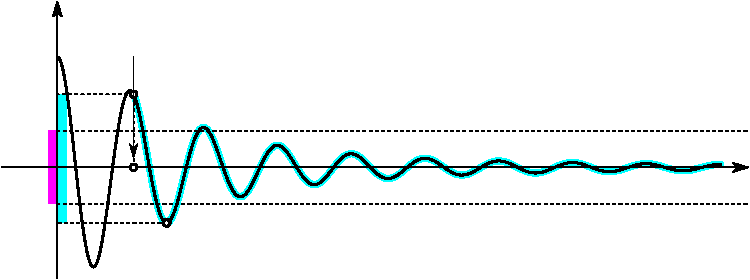
\includegraphics{03ftozeroAtoosmall.pdf}}
        \put( 64.11, 109.07){\sffamily\itshape \makebox[0pt][c]{$A$}}
    \put(  9.52,  68.54){\sffamily\itshape $+\varepsilon$}
    \put(  9.52,  33.53){\sffamily\itshape $-\varepsilon$}
    \put(186.63, 107.07){\sffamily\itshape \makebox[0pt][l]{%
\parbox{2in}{\centering Here $A$ is too small, because\\
 $f(x) > \varepsilon$ happens for some $x\geq A$}}}
\end{picture}


  
    \begin{picture} (360.000000,134.592593)(0,0)
    \put(0.0, 0.0){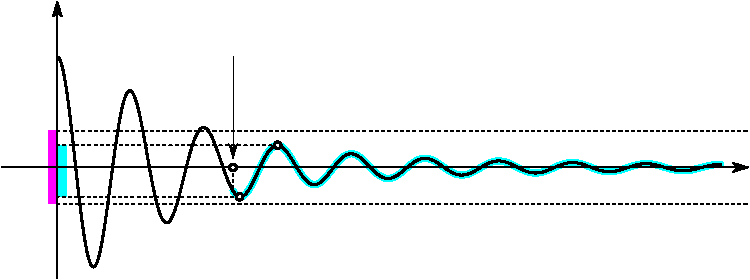
\includegraphics{03ftozeroAok.pdf}}
        \put(111.85, 109.07){\sffamily\itshape \makebox[0pt][c]{$A$}}
    \put(  9.52,  68.54){\sffamily\itshape $+\varepsilon$}
    \put(  9.52,  33.53){\sffamily\itshape $-\varepsilon$}
    \put(186.63, 107.07){\sffamily\itshape \makebox[0pt][l]{%
\parbox{2in}{\centering This $A$ is large enough, because\\
 $f(x)$ is in the right range\\
for all $x\geq A$}}}
\end{picture}

  \caption{The limit of $f(x)$ as $x\to\infty$; how large must $x$ be
    if you need $-\varepsilon < f(x) < \varepsilon$?}
  \label{fig:limit-of-xinv-at-infty}
\end{figure}
\subsection{Example -- Limit of $1/x$} 
\label{ex:lim1overx-at-infty-proved}
The larger $x$ is, the smaller its reciprocal is, so it seems natural that $1/x
\to 0$ as $x\to \infty$.  To \emph{prove} that $\lim_{x\to\infty}1/x = 0$ we
apply the definition to $f(x) = 1/x$, $L=0$.

For a given $\varepsilon>0$, we need to show that
\begin{equation}\label{eq:1overx-small-for-x-large}
  \left|\frac1x - L\right|<\varepsilon \text{ for all } x>A
\end{equation}
provided we choose the right $A$.

How do we choose $A$?  $A$ is not allowed to depend on $x$, but it may
depend on $\varepsilon$.

Let's decide that we will always take $A>0$, so that we only need consider
positive values of $x$.  Then \eqref{eq:1overx-small-for-x-large} simplifies to
\[
\frac 1x<\varepsilon
\]
which is equivalent to
\[
x>\frac1\varepsilon.
\]
This tells us how to choose $A$.  Given any positive $\varepsilon$, we will
simply choose
\[
  A= \text{ the larger of } 0 \text{ and } \frac1\varepsilon
\]
Then we have $|\frac1x-0| = \frac1x <\varepsilon$ for all $x>A$, so we
have proved that $\lim_{x\to\infty}1/x=0$.


\section{Properties of the Limit} 
\label{sec:limitProperties}%
The precise definition of the limit is not easy to use, and
fortunately we don't need to use it very often.  Instead, there
are a number of properties that limits possess that will allow us to compute
complicated limits without having to resort to ``epsiloncy.''

The following properties also apply to the variations on the limit from
\S\ref{sec:variations-on-limit-theme}.  I.e., the following statements remain
true if one replaces each limit by a one-sided limit, or a limit for
$x\to\infty$.  \smallskip

\textbf{Limits of constants and of $x$. } If $a$ and $c$ are constants,
then
\begin{equation}
  \lim_{x\to a}c=c \tag{$P_1$}
\end{equation}
and
\begin{equation}
  \lim_{x\to a} x= a.\tag{$P_2$}
\end{equation}

\textbf{Limits of sums, products, powers, and quotients. } Let $F_1$ and $F_2$ be
two given functions whose limits for $x\to a$ we know,
\[
\lim_{x\to a}F_1(x)=L_1, \qquad \lim_{x\to a}F_2(x)=L_2.
\]
Then
\begin{align*}
  \lim_{x\to a}\bigl(F_1(x)+F_2(x)\bigr) &= L_1+L_2, \tag{$P_3$} \\
  \lim_{x\to a}\bigl(F_1(x)-F_2(x)\bigr) &= L_1 - L_2, \tag{$P_4$} \\
  \lim_{x\to a}\bigl(F_1(x)\cdot F_2(x)\bigr) &= L_1\cdot L_2 . \tag{$P_5$} \\
\end{align*}
If $ \lim_{x\to a}F_2(x)\ne0$, then
\begin{equation}
  \lim_{x\to a}\frac{F_1(x)}{F_2(x)}= \frac{L_1}{L_2}.\tag{$P_6$}
\end{equation}
Finally, if $k$ is an integer, then
\begin{equation}
\lim_{x\to a}\bigl(F_1(x)^k\bigr) = L_1\,^k . \tag{$P_{7}$}
\end{equation}
If $L_1 > 0$, then $(P_7)$ holds for any real number $k$.

In other words ``the limit of the sum is the sum of the limits,'' etc.  One can
prove these laws using the definition of limit in
\S\ref{sec:formal-limit-def} but we will not do this here.  However, these laws
should seem like common sense: if, for $x$ close to $a$, the quantity
$F_1(x)$ is close to $L_1$ and $F_2(x)$ is close to $L_2$, then certainly
$F_1(x)+F_2(x)$ should be close to $L_1+L_2$. (And so forth.)



Later in this chapter we will add two more properties of limits to
this list.  They are the ``Sandwich Theorem''
(\S\ref{sec:limits-and-inequalities}) and the substitution theorem
(\S\ref{sec:continuity}).

\section{Examples of limit computations} 

\subsection{Find $\lim_{x\to2}x^2$} 
We have
\begin{align*}
  \lim_{x\to2} x^2 &= \lim_{x\to2} x\cdot x \\
  &= \bigl( \lim_{x\to2} x\bigr)\cdot \bigl( \lim_{x\to2} x\bigr)
  &\text{by $(P_5)$}\\
  &= 2\cdot 2 = 4.
\end{align*}
Similarly,
\begin{align*}
  \lim_{x\to2} x^3 &= \lim_{x\to2} x\cdot x^2 \\
  &= \bigl( \lim_{x\to2} x\bigr)\cdot \bigl( \lim_{x\to2} x^2\bigr)
  &\text{$(P_5)$ again}\\
  &= 2\cdot 4 = 8,
\end{align*}
and, by $(P_4)$
\[
\lim_{x\to2} x^2-1 = \lim_{x\to2} x^2 - \lim_{x\to2} 1 = 4-1 = 3,
\]
and, by $(P_4)$ again,
\[
\lim_{x\to2} x^3-1 = \lim_{x\to2} x^3 - \lim_{x\to2} 1 = 8-1 = 7,
\]
Putting all this together, we get
\[
\lim_{x\to 2}\frac{x^3-1}{x^2-1} = \frac{2^3-1}{2^2-1} = \frac{8-1}{4-1}=
\frac{7}{3}
\]
because of $(P_6)$.  To apply $(P_6)$ we must check that the denominator
(``$L_2$'') is not zero.  Since the denominator is 3 everything is OK, and
we were allowed to use $(P_6)$.


\subsection{Try the examples \ref{ex:limit-by-sub-good} and \ref{ex:limit-by-sub-bad} using the limit properties} 
To compute $\lim_{x\to 2}(x^2-2x)/(x^2-4)$ we first use the limit
properties to find
\[
\lim_{x\to2} x^2-2x = 0 \text{ and }\lim_{x\to 2}x^2 - 4 = 0.
\]
to complete the computation we would like to apply the last property
$(P_6)$ about quotients, but this would give us
\[
\lim_{x\to2} f(x) = \frac 00.
\]
The denominator is zero, so we were not allowed to use $(P_6)$ (and the
result doesn't mean anything anyway).  We have to do something else.

The function we are dealing with is a \emph{rational function}, which means
that it is the quotient of two polynomials.  For such functions there is an
algebra trick that always allows you to compute the limit even if you
first get $\frac 00$.  The thing to do is to divide numerator and
denominator by $x-2$.  In our case we have
\[
x^2-2x = (x-2)\cdot x, \qquad x^2-4 = (x-2)\cdot (x+2)
\]
so that
\[
\lim_{x\to2} f(x) =\lim_{x\to2} \frac{(x-2)\cdot x } {(x-2)\cdot (x+2)} =
\lim_{x\to2} \frac{x}{x+2}.
\]
After this simplification we \emph{can} use the properties $(P_{\ldots})$
to compute
\[
\lim_{x\to2} f(x) = \frac{2}{2+2} = \frac12.
\]

\subsection{Example -- Find $\lim_{x\to 2}\sqrt x$} 
\label{ex:limit-of-sqrt-at-2}
  We can apply limit property $(P_{5a})$ with $k=1/2$ to see that
\[
  \lim_{x\to2} \sqrt{x} = \lim_{x\to2} x^{1/2} = [\lim_{x\to2} x]^{1/2} =
  2^{1/2} = \sqrt{2}.
\]

\subsection{Example -- The derivative of $\sqrt x$ at $x=2$} 
Find
\[
\lim_{x\to2}\frac{\sqrt x-\sqrt2}{x-2}
\]
assuming the result from the previous example (i.e., assuming that
$\lim_{x\to2}\sqrt x = \sqrt2$.)

\textit{Solution: } The function is a fraction whose numerator and
denominator vanish when $x=2$, so the limit is of the form ``$\frac00$''.
We use an algebra trick; namely, multiplying the numerator and
denominator by $\sqrt{x}+\sqrt{2}$:
\[
\frac{\sqrt x-\sqrt2}{x-2}
= \frac{(\sqrt x-\sqrt2)(\sqrt{x}+\sqrt{2})}{(x-2)(\sqrt
  x+\sqrt2)} =\frac{1}{\sqrt x+\sqrt2}.
\]
Now we can use the limit properties to compute
\[
\lim_{x\to2} \frac{\sqrt x-\sqrt 2}{x-2} = \lim_{x\to2} \frac{1}{\sqrt
  x+\sqrt 2} =\frac1{2\sqrt2} =\frac{\sqrt2}4.
\]



\subsection{Limit as $x\to\infty$ of Rational Functions} 
\label{sec:lim-at-infty-of-rationalfunction}%
A rational function is the quotient of two polynomials:
\begin{equation}\label{eq:your-typical-rational-function}
  R(x) = \frac{a_nx^n+\cdots +a_1x+a_0}{b_mx^m+\cdots+b_1x+b_0}.
\end{equation}
We have seen that
\[
\lim_{x\to\infty} \frac 1x =0
\]
We even proved this in example \ref{ex:lim1overx-at-infty-proved}.  Using
this we can find the limit at $\infty$ for any rational function $R(x)$ as
in \eqref{eq:your-typical-rational-function}.  We could turn the outcome
of the calculation of $\lim_{x\to\infty}R(x)$ into a boxed recipe
involving the degrees $n$ and $m$ of the numerator and denominator, and
also their coefficients $a_i$, $b_j$, which you, the student, would then memorize,
but it is better to remember {\itshape the trick:}
\begin{verse}\itshape
  To find the limit as $x\to\infty$,\\
  of some rational function you have been given,\\
  factor the highest occurring powers of $x$,\\
  both from numerator and from denominator.
\end{verse}
For example, let's compute
\[
\lim_{x\to\infty}\frac{3x^2+3}{5x^2+7x-39}.
\]
Remember the trick and factor $x^2$ from top and bottom. You get
\begin{align*}
  \lim_{x\to\infty}\frac{3x^2+3}{5x^2+7x-39}
  &= \lim_{x\to\infty}\frac{x^2}{x^2} \; \frac{3+3/x^2}{5+7/x-39/x^2}
  & \text{(algebra)}\\
  &= \lim_{x\to\infty}\frac{3+3/x^2}{5+7/x-39/x^2}& \text{(more algebra)}\\
  &= \frac{\lim_{x\to\infty}(3+3/x^2)}{\lim_{x\to\infty}(5+7/x-39/x^2)}
  &\text{(limit properties)}\\
  &= \frac35.
\end{align*}
At the end of this computation, we used the limit properties
$(P_\ast)$ to break the limit down into simpler pieces like
$\lim_{x\to\infty}39/x^2$, which we can directly evaluate; for example, we have
\[
\lim_{x\to\infty} 39/x^2 =\lim_{x\to\infty} 39\cdot \left( \frac1x
\right)^2 = \left( \lim_{x\to\infty}39\right)\cdot \left(
  \lim_{x\to\infty}\frac1x \right)^2 = 39 \cdot 0^2 =0.
\]
  The other terms are similar.
  
  
\subsection{Another example with a rational function} 
Compute
\[
\lim_{x\to\infty} \frac {2x}{4x^3+5}.
\]
We apply ``the trick'' again and factor $x$ out of the numerator and
$x^3$ out of the denominator.
This leads to
\begin{align*}
  \lim_{x\to\infty} \frac {2x}{4x^3+5}
  &=\lim_{x\to\infty} \Bigl(\frac{x}{x^3}\;\frac{2}{4+5/x^3}\Bigr)\\
  &=\lim_{x\to\infty} \Bigl(\frac{1}{x^2}\;\frac{2}{4+5/x^3}\Bigr)\\
  &=\lim_{x\to\infty} \Bigl(\frac{1}{x^2}\Bigr)\cdot \Bigl(\lim_{x\to\infty}\frac{2}{4+5/x^3}\Bigr)\\
  &=0\cdot \tfrac24\\
  &=0.
\end{align*}
This example and the previous cover two of the three possible
combinations of degrees $n$ and $m$, namely $n=m$ and $n<m$.  To show
the remaining case, in which the numerator has higher degree than the
denominator, we should do yet another example, but that one will have
to wait a few pages (see
\S~\ref{sec:03infinite-limit-of-rational-functions})


\section{When limits fail to exist} 
In the last couple of examples we worried about the possibility that a
limit $\lim_{x\to a}g(x)$ actually might not exist.  This can actually
happen, and in this section we'll see a few examples of what failed limits
look like.  First let's agree on what we will call a ``failed limit.''

\subsection{Definition} 
\itshape
If there is no number $L$ such that $\lim_{x\to a}f(x) = L$, then we say
that the limit $\lim_{x\to a}f(x)$ does not exist.  \upshape


\subsection{The sign function near $x=0$} 
\label{sec:sign-function-has-no-limit}
The ``sign function'' is defined by%
\marginpar{\footnotesize\sffamily\raggedleft 
    \begin{picture} (90.000000,42.228571)(0,0)
    \put(0.0, 0.0){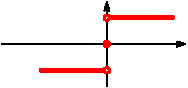
\includegraphics{03signOFx.pdf}}
        \put( 48.29,  31.69){\sffamily\itshape \makebox[0pt][r]{$1$}}
    \put( 53.29,   6.54){\sffamily\itshape \makebox[0pt][l]{$-1$}}
\end{picture}
\\[1ex]
  $y=\sign(x)\hfill\null$\\
  There are those who do not like the notation
  ``$\sign(x)$,'' and prefer to write\\
  $g(x) = \frac{x}{|x|}$
  instead of $g(x) = \sign(x)$.  If you think about this formula for a
  moment you'll see that $\sign(x)$ and $ x/|x|$ are the same for all
  $x\neq0$.  When $x=0$ the quotient $x/|x|$ is of course not defined.
}%
\[
\sign (x) =
\begin{cases}
  -1 & \text{for $x<0$}\\ 0 & \text{for $x=0$}\\ 1 & \text{for $x>0$}
\end{cases}
\]
Note that ``the sign of zero'' is defined to be zero.  Our question is: does the
sign function have a limit at $x=0$?  The answer is \emph{no}, and here is why:
since $\sign(x) = +1$ for all positive values of $x$, we see that
\[
 lim_{x\searrow 0} \sign(x) = +1.
\]
Similarly, since $\sign(x) = -1$ for all negative values of $x$, we see that
\[
 lim_{x\nearrow 0} \sign(x) = -1.
\]
 Then by the result of \ref{one_sided_limit_thm}, we see that because the two one-sided limits have different values, the two-sided limit does not exist.  (Essentially, if the two-sided limit existed, then it would have to be equal to both $+1$ and $-1$ at the same time, which is impossible.)
\[
\text{Conclusion:}\quad
\lim_{x\to 0} \sign (x) \text{ does not exist.}
\]
\subsection{The example of the backward sine} 
\label{sec:03backward-sine}
Contemplate the limit as $x\to0$ of the ``backward sine,'' i.e.
\[
\lim_{x\to 0}\sin \Bigl(\frac\pi x\Bigr).
\]

When $x=0$ the function $f(x)=\sin(\pi /x)$ is not defined, because its
definition involves division by $x$.  What happens to $f(x)$ as $x\to0$?
First, $\pi /x$ becomes larger and larger (``goes to infinity'') as
$x\to0$.  Then, taking the sine, we see that $ \sin(\pi /x)$ oscillates
 between $+1$ and $-1$ infinitely often as $x\to0$, since, for example, we can calculate that $f(\frac{2}{4k+1})=+1$ and $f(\frac{2}{4k+3})=-1$ for each integer $k$. This means that $f(x)$
gets close to any number between $-1$ and $+1$ as $x\to0$, but that the
function $f(x)$ \emph{never stays close} to any particular value because it
keeps oscillating up and down between $+1$ and $-1$.

\begin{figure}[ht]\centering
  \input ../figures/221/03sinePiOverx.tex
  \caption{Graph of $y = \sin\frac\pi x$ for $-3<x<3$,\ \ $x\neq0$.}
  \label{fig:03sinePiOverx}
\end{figure}

Here again, the limit $\lim_{x\to0}f(x)$ does not exist.  We have arrived
at this conclusion by only considering what $f(x)$ does for small positive
values of $x$.  So the limit fails to exist in a stronger way than in the
example of the sign-function. There, even though the limit didn't exist,
the one-sided limits existed.  In the present example we see that even the
one-sided limits
\[
  \lim_{x\searrow 0} \sin \Bigl(\frac{\pi}{x} \Bigr)
  \text{ and }
  \lim_{x\nearrow 0} \sin \Bigl(\frac{\pi}{x} \Bigr)
\]
do not exist.
\subsection{Limit properties for limits that don't exist} 
The limit properties all say that some limit exists (and what it's equal to),
but by applying some logic you can sometimes also use the limit properties to
conclude that a limit does \emph{not} exist.  For instance:
\subsection*{Theorem}% lim g+h doesn't exist implies either limg or limh fails 
\itshape
If $\lim_{x\to a}f(x) + g(x)$ does not exist, then at least one of the
two limits $\lim_{x\to a}f(x)$ or $\lim_{x\to a}g(x)$ does not exist.
\upshape\medskip
\noindent%
In English: ``if the sum of two functions has no limit, then one of
the terms also has no limit.''
This follows directly from Property $(P_3)$ which says that if $\lim
f(x)$ and $\lim g(x) $ both exist then $\lim f(x)+g(x)$ also must
exist.
\section{Limits that equal $\infty$} 
\label{sec:03limits-that-equal-infty}
For some limits that don't exist, we can be more descriptive about the
reason that the limit doesn't exist.  Here are some examples.

\subsection{The limit of $1/x$ at $x=0$} 
\label{sec:limit-1x-at-zero}
Consider the limit
\[
\lim_{x\to 0} \frac{1} {x}.
\]
As $x$ decreases to $x=0$ through smaller and smaller positive values,
its reciprocal $1/x$ becomes larger and larger.  We say that instead
of going to some finite number, the quantity $1/x$ ``goes to
infinity'' as $x\searrow0$.  In symbols:
\begin{equation}
  \lim_{x\searrow 0} \frac{1} {x} = \infty.
  \label{eq:03limit-invx-is-infty}  
\end{equation}%
\marginpar{\input ../figures/221/03inverse-of-x.tex }%
Likewise, as $x$ approaches $0$ through negative numbers, its
reciprocal $1/x$ drops lower and lower, and we say that $1/x$ ``goes
to $-\infty$'' as $x\nearrow 0$.  Symbolically,
\begin{equation}
  \label{eq:03limit-invx-is-neg-infty}
    \lim_{x\nearrow 0} \frac{1} {x} = -\infty.
\end{equation}
The limits \eqref{eq:03limit-invx-is-infty} and
\eqref{eq:03limit-invx-is-neg-infty} are not like the normal limits we
have been dealing with so far.  Namely, when we write something like
\[
\lim_{x\to2} x^2 = 4
\]
we mean that the limit actually exists and that it is equal to $4$.
On the other hand, since we have agreed that $\infty$ is not a number,
the meaning of \eqref{eq:03limit-invx-is-infty} cannot be to say that
``the limit exists and its value is $\infty$.''

Instead, when we write
\begin{equation}
  \lim_{x\to a} f(x) = \infty
  \label{eq:03limit-of-f-infty}
\end{equation}
for some function $y=f(x)$, we mean, \emph{by definition,} that the
limit of $f(x)$ does not exist, and that it fails to exist in a
specific way: as $x\to a$, the value of $f(x)$ becomes ``larger and
larger,'' and in fact eventually becomes larger than any finite
number.

The language in that last paragraph shows you that this is an
intuitive definition, at the same level as the first definition of
limit we gave in \S\ref{sec:informal-limit-def}.  It contains the
usual suspect phrases such as ``larger and larger,'' or ``finite
number'' (as if there were any other kind.)  A more precise definition
involving epsilons can be given, but in this course we will not go
into this much detail.  As a final comment on infinite limits, it is
important to realize that, since \eqref{eq:03limit-of-f-infty} is not
a normal limit \emph{you cannot apply the limit rules to infinite
  limits. }  Here is an example of what goes wrong if you try anyway.

\subsection{Trouble with infinite limits} 
\label{sec:trouble-with-infinite-limits}
If you apply the limit properties to $\lim_{x\searrow0} 1/x = \infty$,
then you could conclude
\[
1 = \lim_{x\searrow 0} x\cdot \frac{1} {x}
 = \lim_{x\searrow 0} x \times \lim_{x\searrow 0}  \frac{1} {x}
 = 0 \times \infty
 = 0,
\]
because ``anything multiplied with zero is zero.''

After using the limit properties in combination with this infinite
limit we reach the absurd conclusion that $1=0$.  The moral of this
story is that you can't use the limit properties when some of the
limits are infinite.
% !!! Issue: This discussion of algebraic properties of infinite limits needs to
% be redone. It is extremely wrong not to explain why 2 times infinity is
% infinity. What should be done is to say the limit rules do hold, except that 0
% times infinity, infinity minus infinity, 0/0, and infinity / infinity are
% undefined. This would also fix the massive problems with the next example
% about rational functions.
\subsection{Limit as $x\to\infty$ of rational functions, again} 
\label{sec:03infinite-limit-of-rational-functions}
In \S~\ref{sec:lim-at-infty-of-rationalfunction} we computed the
limits of rational functions $R(x) = \frac{P(x)} {Q(x)}$ as
$x\to\infty$ in all cases where the degree of the numerator $P$ was
not more than the degree of the denominator $Q$.  Here we complete the
story by looking at the remaining case where $\deg P > \deg Q$.
We'll do the following examples:
\[
  A = \lim_{x\to\infty} x, \quad
  B = \lim_{x\to\infty} -7x^2, \quad
  C = \lim_{x\to\infty} \frac{x^3-2x} {1+25x^2}.
\]
The first limit is the easiest: ``as $x$ goes to infinity, $x$ goes to
infinity.''  So we have
\[
A = \lim_{x\to\infty} x = \infty.
\]
Remember, we don't have a precise definition that says when a limit
equals ``$\infty$,'' so we can't prove this here.  On the other hand,
if someone were to come up with a definition of the above limit that
would make it equal to something else, we would ask them to change
their definition instead of changing our mind about $\lim_{x\to\infty}
x$.
The second limit is only slightly harder: as $x\to\infty$, the square
$x^2$ also becomes arbitrarily large, and thus $-7x^2$ will go to
$-\infty$.  So we'll say  $B=-\infty$.
Finally, let's look at $C$.  We apply the trick from
\S~\ref{sec:lim-at-infty-of-rationalfunction}:
\[
C = \lim_{x\to\infty}  \frac{x^3-2x} {1+25x^2}
=  \lim_{x\to\infty} \frac{x^3} {x^2}  \frac{1-\frac2x} {\frac1x+25}.
\]
At this point we would like to use the limit properties to say
\[
C =  \lim_{x\to\infty} \frac{x^3} {x^2}  \frac{1-\frac2x} {\frac1x+25}
= \lim_{x\to\infty} \frac{x^3} {x^2}\; \lim_{x\to\infty}
\frac{1-\frac2x} {\frac1x+25}
=\bigl(\lim_{x\to\infty} x\bigr) \cdot \frac{1} {25}
=\infty \cdot \frac{1} {25}
=\infty.
\]
Unfortunately, as we have just seen, the limit properties are
unreliable when infinite limits are involved, so we have no
justification for using them here.  Nevertheless, the answer we got
this time seems reasonable; in an attempt to make it look more
reasonable you could write it this way:
\[
\frac{x^3} {x^2}  \frac{1-\frac2x} {\frac1x+25}
=x\cdot \frac{1-\frac2x}{\frac1x+25}
\approx x \cdot \frac{1} {25}
\]
for large $x$.  Therefore, as $x\to\infty$ the fraction
\[
\frac{x^3} {x^2}  \frac{1-\frac2x} {\frac1x+25}
\approx x \cdot \frac{1} {25}
\to\infty.
\]
% !!! Issue: This is also really bad style: what does "approximately equals"
% even mean here?!?
\section{What's in a name? -- Free Variables and Dummy variables} 
  % !!! Discuss: Should this section appear earlier, right near the definition of limit?
\label{sec:free-versus-dummy-variables}%
There is a big difference between the variables $x$ and $a$ in the formula
\[
\lim_{x\to a} 2x+1,
\]
namely $a$ is a \emph{free variable}, while $x$ is a \emph{dummy variable}
(or ``placeholder'' or a ``bound variable.'')

The difference between these two kinds of variables is this:
\begin{itemize}
\item if you replace a dummy variable in some formula consistently by some
  other variable then the value of the formula does not change.  On the
  other hand, it never makes sense to substitute a number for a dummy
  variable.

\item the value of the formula may depend on the value of the free
  variable.
\end{itemize}
To understand what this means consider the example $\lim_{x\to a}2x+1$
again.  The limit is easy to compute:
\[
\lim_{x\to a}2x+1 = 2a+1.
\]
If we replace $x$ by, say $u$ (systematically) then we get
\[
\lim_{u\to a} 2u+1
\]
which is again equal to $2a+1$.  This computation says that \textit{if some
  number gets close to $a$ then two times that number plus one gets close
  to $2a+1$.}  This is a very wordy way of expressing the formula, and you
can shorten things by giving a name (like $x$ or $u$) to the number that
approaches $a$.  But the result of our computation shouldn't depend on the
name we choose: it doesn't matter if we call it $x$ or $u$, or anything else.
Some prefer to call $x$ a bound variable, meaning that in
\[
\lim_{x\to a} 2x+1
\]
the $x$ in the expression $2x+1$ is bound to the $x$ written underneath the
limit -- you can't change one without changing the other.

Substituting a number for a dummy variable usually leads to complete
nonsense.  For instance, let's try setting $x=3$ in our limit: what is
\[
\lim_{3\to a}2\cdot 3+1\,?
\]
Of course $2\cdot 3+1 = 7$, but what does $7$ do when $3$ gets closer and
closer to the number $a$?  That's a silly question, because 3 is a constant
and it doesn't ``get closer'' to some other number like $a$!  (If you ever
see 3 get closer to another number then it's time to take a vacation!)

On the other hand the variable $a$ is free: you can assign it particular
values, and its value will affect the value of the limit.  For instance, if
we set $a=3$ (but leave $x$ alone), then we get
\[
\lim_{x\to 3} 2x+1
\]
and there's nothing strange about that, since the limit is $2\cdot3+1=7$ (no
problem).  We could substitute other values of $a$ and we would get
different answers. In general you get $2a+1$.

\section{Limits and Inequalities} 
\label{sec:limits-and-inequalities}%
This section has two theorems that let you compare limits of different
functions.  The properties in these theorems are not formulas that
allow you to compute limits like the properties $(P_1)$\ldots$(P_6)$
from \S\ref{sec:limitProperties}.  Instead, they allow us to
\emph{reason} about limits.

The first theorem should not surprise you --- all it says is that bigger
functions have bigger limits.

\subsection{Theorem} 
\itshape
Let $f$ and $g$ be functions whose limits as $x\to a$ exist, and assume
that $f(x)\leq g(x)$ holds for all $x$.  Then
\[
\lim_{x\to a}f(x) \leq \lim_{x\to a} g(x).
\]
\upshape

A useful special case arises when we set $f(x)=0$.  The theorem then says
that if a function $g$ never has negative values, then its limit will also
never be negative.
Here is the second theorem about limits and inequalities.

\subsection{The Sandwich Theorem} 
\itshape
Suppose that
\[
f(x)\le g(x)\le h(x)
\]
(for all $x$) and that both the limits
\[
  \lim_{x\to a} f(x) \text{ and } \lim_{x\to a} h(x)
\]
exist and are equal to the same value $L$. Then
\[
\lim_{x\to a} g(x)
\]
also exists and is equal to $L$.
\upshape

The theorem is useful when we want to know the limit of $g$, and when we
can \emph{sandwich} it between two functions $f$ and $h$ whose limits are
easier to compute.  The Sandwich Theorem looks like the first theorem of
this section, but there is an important difference: in the Sandwich Theorem
we don't have to assume that the limit of $g$ exists.  The inequalities
$f\leq g\leq h$ combined with the circumstance that $f$ and $h$ have the
same limit are enough to guarantee that the limit of $g$ exists.

\begin{figure}[h]\centering
  \input ../figures/221/03backwardCosSandwich.tex
  \caption{The graph of  $x\cos\frac\pi x$ is ``sandwiched'' in
    between the graphs of $y=+|x|$ and of $y=-|x|$.}
  \label{fig:03backwardCosSandwich}
\end{figure}

\subsection{Example: a Backward Cosine Sandwich. }
\label{sec:backward-cosine-sandwich}
  % Why wouldn't we use sine, because that's what we did earlier ?!?!?
\label{sec:03xcos1overx} The Sandwich Theorem says that if the function
$g(x)$ is sandwiched between two functions $f(x)$ and $h(x)$ and the limits
of the outside functions $f$ and $h$ exist and are equal, then the limit of
the inside function $g$ exists and equals this common value.  For example
\[
-|x|\le x\cos\frac\pi x\le |x|
\]
since the cosine is always between $-1$ and $1$. Since
\[
\lim_{x\to 0}-|x|=\lim_{x\to 0}|x|=0,
\]
the Sandwich Theorem tells us that
\[
\lim_{x\to 0} x\cos\frac\pi x =0.
\]
Note that the limit $ \lim_{x\to 0} \cos(\pi/x) $ does \emph{not}
exist, for the same reason that the ``backward sine'' did not have a
limit for $x\to0$ (see \S~\ref{sec:03backward-sine}).  Multiplying
with $x$ changed that.



\section{Continuity} 
\label{sec:continuity}

\subsection{Definition} 
\label{sec:03def-continuity}\itshape
A function $g$ is \emph{continuous} at $a$ if
\begin{equation}\label{eq:continuity-def}
  \lim_{x\to a} g(x) = g(a)
\end{equation}
A function is continuous if it is continuous at every $a$ in its
domain.\upshape\medskip
% This is the wrong definition of continuity: 1/x is not "a continuous function" in any reasonable sense. The right definition is if the function is continuous on the closure of its domain, or something.
Note that when we say that ``a function is continuous on some
interval'' it has to be defined on that interval. For example, the
function $f(x)=1/x^2$ is continuous on the interval $1<x<5$ but is
\emph {not} continuous on the interval $-1<x<1$ because it isn't
defined at $x=0$.
Continuous functions are ``nice'', and most functions we will want to talk about
will be continuous.  For example, all polynomials are continuous functions. The
ideas in the proof are the same as in the following example
\subsection{Example.  A polynomial that is continuous} 
Let us show that $P(x) = x^2+3x$ is continuous at $x=2$.  To
show that we have to prove that
\[
\lim_{x\to 2} P(x) = P(2),
\]
which is to say,
\[
\lim_{x\to 2}x^2+3x = 2^2+3\cdot 2.
\]
We can do this two ways: using the definition with $\varepsilon$ and
$\delta$ (the hard way).  It is much easier to the limit properties
$(P_1)$\ldots $(P_6)$ from \S\ref{sec:limitProperties}: for example,
\begin{align*}
  \lim_{x\to 2}x^2+3x &= \lim_{x\to 2}x^2 + \lim_{x\to 2} 3x \\
  &= (\lim_{x\to 2}x )\cdot (\lim_{x\to 2}x ) + (\lim_{x\to 2}3)\cdot (\lim_{x\to 2}x)\\
  &= 2 \cdot 2 + 3 \cdot 2
\end{align*}
and this is what we wanted.
% !!! TO-WRITE: We need a subsection here listing the properties of continuous functions: sum, product, quotient, composition, powers, inverses of continuous are continuous.
  
\subsection{Example.  Rational functions are continuous wherever they are defined} 

Let $R(x) = \frac{P(x)}{Q(x)}$ be a rational function, and let $a$ be any
number in the domain of $R$; i.e., any number for which $Q(a)\neq0$.  Then
one has
\begin{align*}
  \lim_{x\to a}R(x)
  &= \lim_{x\to a}\frac{P(x)}{Q(x)} && \\
  &= \frac{\lim_{x\to a} P(x)}{\lim_{x\to a}Q(x)}
  && \text{property }(P_6)\\
  &= \frac{P(a)}{Q(a)} && \text{$P$ and $Q$ are continuous}\\
  &= R(a).
\end{align*}
This shows that $R$ is indeed continuous at $a$.
% !!! Issue: How about sine and cosine? The fact that these functions are continuous is important, and in fact it is implicitly assumed several times later.

\subsection{Example of a discontinuous function} 
Here is an artificial example of a discontinuous function.  Consider  
\[
f(x) =
\begin{cases}
  0 & \text{ when } x\neq0 \\
  1 & \text{ when } x=0
\end{cases}.
\]%
\marginpar{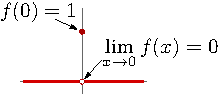
\includegraphics{03simple_discontinuity.pdf}}%
This function is not continuous at $x=0$ because $\lim_{x\to0} f(x) =
0$, while $f(0) = 1$: the limit for $x\to0$ exists, but it is
different from the function value at $x=0$.

This example is artificial, because we took a continuous function
($f(x) = 0$) and changed its definition at one point ($f(0) = 1$),
which then made the function discontinuous.  We get less artificial
examples by looking at functions that do not have limits.  If
$\lim_{x\to a} g(x)$ does not exist, then it certainly cannot be equal
to $g(a)$, and therefore any failed limit provides an example of a
discontinuous function.

For instance, the sign function $g(x) = \sign(x)$ from
\S~\ref{sec:sign-function-has-no-limit} is not continuous at $x=0$.
This kind of discontinuity is fairly common and has a name:
\marginpar{\input ../figures/221/03signOFx.tex\\
  \footnotesize\sffamily%
  $y=\sign (x)$: a function with a jump discontinuity.  Left and right
  limits at $x=0$ exist, but they are not the same}

\subsection{Definition}% of Jump discontinuity 
\itshape  A function $y=f(x)$ has a \emph{jump discontinuity} at $x=a$
if the left- and right-hand limits of $f(x)$  at $x=a$ both exist but are
different:
\[
\lim_{x\nearrow a} f(x) \neq \lim_{x\searrow a} f(x).
\]
\upshape

\subsection{Removable discontinuities} 
\label{sec:removable-discontinuities}
Consider the function from \S~\ref{sec:03xcos1overx}
\[
f(x) = x\cos\frac{\pi} {x}.
\]
It is defined for all $x$ except $x=0$, and therefore it is not continuous at
$x=0$, but for the silly reason that $f$ is not defined there: to decide if $f$
is continuous at $x=0$ we must compare $\lim_{x\to0} f(x)$ with $f(0)$,
but $f(0)$ isn't defined.  However, the limit
\[
\lim_{x\to 0} f(x) =\lim_{x\to 0} x \cos\frac{\pi} {x} = 0
\]
does exist (by the Sandwich theorem, see \S~\ref{sec:03xcos1overx}
again).
\marginpar{\input ../figures/221/03backwardCosSandwichSmall.tex}
Since $f(0)$ is not defined yet we can extend the
definition of $f$ to include $f(0) = 0$, i.e., we define
\[
g(x) =
\begin{cases}
  x\cos \pi/x & \text{ for }x\neq0\\
  0 & \text{ when }x=0 .
\end{cases}
\]
This new function $g(x)$ then is continuous everywhere, including at $x=0$.

This is an example of a more general situation in which the domain of
a function ``has a hole,'' meaning that the function is defined
everywhere in some interval $a-\delta <x < a+\delta$, except at $x=a$.
If the limit $\lim_{x\to a} f(x) = L$ exists, then you can extend the
definition of the function by declaring that $f(a) = L$.  The extended
function is then continuous at $x=a$.  The point $x=a$ is called a
\emph{removable discontinuity} of the function $f$.  In
\S~\ref{sec:another-example-of-removable-discontinuity} we'll see
another example of a function with a removable discontinuity whose
graph isn't as messy as the graph of $x\cos\pi/x$.


\section{Substitution in Limits} 
\label{sec:substitution-in-limits} Given
two functions $f$ and $g$, we can consider their composition $h(x) = f(g(x))$.
To compute the limit
\[
\lim_{x\to a} f\bigl(g(x)\bigr)
\]
we let $u=g(x)$, so that we want to know
\[
\lim_{x\to a}f(u) \text{ where }u=g(x).
\]
If we can find the limits
\[
L = \lim_{x\to a} g(x)\text{ and } \lim_{u\to L} f(u) = M,
\]
Then it seems reasonable that as $x$ approaches $a$, $u=g(x)$ will approach
$L$, and $f(g(x))$ approaches $M$.
This is in fact a theorem:
\subsection{Theorem} 
\label{thm:substitution}%
\itshape%
If $\lim_{x\to a}g(x) = L$, and if the function $f$ is continuous at $u=L$,
then
\[
\lim_{x\to a}f\bigl(g(x)\bigr) = \lim_{u\to L}f(u) = f(L).
\]\upshape

Another way to write this is
\[
\lim_{x\to a}f\bigl(g(x)\bigr) = f\bigl(\lim_{x\to a}g(x)\bigr).
\]
What this statement means is that we can freely move continuous functions outside of limits.
\subsection{Example: compute $\lim_{x\to3}\sqrt{x^3-3x^2+2}$} 
The given function is the composition of two functions, namely
\[
\sqrt{x^3-3x^2+2} = \sqrt u, \text{ with } u = x^3-3x^2+2,
\]
or, in function notation, we want to find $\lim_{x\to 3}h(x)$ where
\[
h(x) = f(g(x)), \text{ with } g(x) = x^3-3x^2+2\text{ and }f(x) = \sqrt{x}.
\]
Either way, we have
\[
\lim_{x\to 3}x^3-3x^2+2 = 2\quad\text{and}\quad \lim_{u\to 2}\sqrt u =
\sqrt 2.
\]
We can get the first limit from the limit properties $(P_1)$\ldots$(P_5)$.
The second limit says that taking the square root is a continuous function,
which it is. We have not proved this is true, but this particular limit is
the one from example \ref{ex:limit-of-sqrt-at-2}.  Putting these two limits
together, we conclude that the limit is $\sqrt2$.
% NOTE: if the subsection on continuous functions is written, rewrite this example!
We could more compactly write this whole argument as follows:
\[
\lim_{x\to3}\sqrt{x^3 - 3x^2 + 2} =\sqrt{\lim_{x\to 3}x^3 - 3x^2 + 2}
=\sqrt 2,
\]
with the remark that we need to know that $f(x)=\sqrt x$ is a continuous
function to justify the first step.

Another possible way of writing this is
\[
\lim_{x\to3}\sqrt{x^3 - 3x^2 + 2} =\lim_{u\to 2}\sqrt u =\sqrt2,
\]
where we would need to say that we have substituted $u=x^3-3x^2+2$.

\section{Problems} 
\problemfont 
\textit{Find the following limits:}\\
% !!! Issue: Some of these problems require "bad infinite limit reasoning" like in the subsection on that stuff.
\begin{multicols}{3}\setlength{\parindent}{0pt}

\problem $\DS \lim_{x\to -7}(2x+5) $ 

\problem $\DS \lim_{x\to 7-}(2x+5) $ 

\problem $\DS \lim_{x\to -\infty}(2x+5) $ 

\problem $\DS \lim_{x\to-4} (x+3)^{2006} $ 

\problem $\DS \lim_{x\to-4} (x+3)^{2007} $ 

\problem $\DS \lim_{x\to-\infty} (x+3)^{2007}$ 

\problem $\DS \lim_{t\to1}\frac{t^2+t-2}{t^2-1} $ 

\problem $\DS \lim_{t\nearrow1}\frac{t^2+t-2}{t^2-1} $ 

\problem $\DS \lim_{t\to-1}\frac{t^2+t-2}{t^2-1} $ 

\problem $\DS \lim_{x\to\infty}\frac{x^2+3}{x^2+4} $ 

\problem $\DS \lim_{x\to\infty}\frac{x^5+3}{x^2+4} $ 

\problem $\DS \lim_{x\to\infty}\frac{x^2+1}{x^5+2} $ 

\problem $\DS \lim_{x\to\infty} \frac{(2x+1)^4}{ (3x^2+1)^2} $ 

\problem $\DS \lim_{u\to\infty} \frac{(2u+1)^4}{ (3u^2+1)^2} $ 

\problem $\DS \lim_{t\to0} \frac{(2t+1)^4}{ (3t^2+1)^2}$ 
\end{multicols}
\problem What are the coordinates of the points labeled $A$, \ldots, $E$ in 
Figure~\ref{fig:03sinePiOverx} (the graph of $y=\sin\pi/x$).
\answer 
$A (\frac23,-1)$; $B (\frac25, 1)$; $C (\frac27,-1)$; $D(-1,0)$;
$E(-\frac25, -1)$.
\endanswer
% TO-DO: Combine all 10 or so of the true-false problems into one problem.
\problem If $\lim_{x\to a} f(x)$ exists then $f$ is continuous at $x=a$. 
\textit{True or false?}
\answer 
False!  The limit must not only exist \textit{but also be equal to
}$f(a)$!
\endanswer

\problem Give two examples of functions for which $\lim_{x\searrow 0} 
f(x)$ does not exist.
\answer 
There are of course many examples.  Here are two: $f(x) = 1/x$ and
$f(x) = \sin(\pi/x)$ (see \S\ref{sec:03backward-sine})
\endanswer

\problem \groupproblem If $\lim_{x\to 0}f(x)$ and $\lim_{x\to0}g(x)$ both do not 
exist, then $\lim_{x\to 0}\bigl(f(x) + g(x)\bigr)$ also does not exist.
\textit{True or false?}

\answer 
False!  Here's an example: $f(x) = \frac1x$ and $g(x) = x-\frac1x$.
Then $f$ and $g$ don't have limits at $x=0$, but $f(x) + g(x) = x$
\textit{does} have a limit as $x\to0$.
\endanswer

\problem \groupproblem If $\lim_{x\to 0}f(x)$ and $\lim_{x\to0}g(x)$ both do not 
exist, then $\lim_{x\to 0}(f(x)/g(x))$ also does not exist.  \textit{True or false?}

\answer 
False again, as shown by the example $f(x) = g(x) = \frac1x$.
\endanswer

\problem True or false: 

\subprob If $\lim_{x\to a} f(x)$ exists and $\lim_{x\to a} g(x)$ does
not exist, then $\lim_{x\to a} f(x) + g(x)$ could still exist.
\answer 
False, for the following reason:  $g(x)$ is the difference of $f(x)+g(x)$ and
$f(x)$.  If $\lim_{x\to a} f(x)$ exists and $\lim_{x\to a} f(x) + g(x)$ also exists, then
\begin{align*}
  \lim_{x\to a} g(x) &= \lim_{x\to a} \bigl\{f(x) + g(x) - f(x)\bigr\}\\
  &= \lim_{x\to a} \bigl\{f(x) + g(x)\bigr\} - \lim_{x\to a} f(x)
\end{align*}
also has to exist.
\endanswer

\subprob If $\lim_{x\to a} f(x)$ exists and $\lim_{x\to a} g(x)$ does
not exist, then $\lim_{x\to a} f(x) g(x)$ could still exist.
\answer 
True, as shown by the example $f(x) = x$, $g(x) = \frac{1}{x}$, and $a=0$.
For these two functions we have
\begin{gather*}
  \lim_{x\to 0} f(x) = 0 \text{ (i.e.\ exists) } \\
  \lim_{x\to 0} g(x) = \text{ does not exist } \\
  \lim_{x\to 0} f(x) g(x) = \lim_{x\to 0} x\times\frac1x = 1 \text{ (i.e.\
  exists) }
\end{gather*}
You can make up other examples, but to show that this statement is true you only
need one example.
\endanswer

\subprob If $\lim_{x\to a} f(x)$ exists and $\lim_{x\to a} g(x)$ does
not exist, then $\lim_{x\to a} f(x)/g(x)$ could still exist.
\answer 
True, as shown by the same example $f(x) = x$, $g(x) = \frac{1}{x}$, $a=0$.
This time we have
\begin{gather*}
  \lim_{x\to 0} f(x) = 0 \text{ (i.e.\ exists) } \\
  \lim_{x\to 0} g(x) = \text{ does not exist } \\
  \lim_{x\to 0} \frac{f(x)}{g(x)} = \lim_{x\to 0} \frac{x}{1/x} =\lim_{x\to0}
  x^2 = 0 \text{ (i.e.\ exists) }
\end{gather*}
You can make up other examples, but to show that this statement is true you only
need one example.
\endanswer

\subprob If $\lim_{x\to a} f(x)$ does not exist but $\lim_{x\to a} g(x)$ does
exist, then $\lim_{x\to a} f(x)/g(x)$ could still exist.
\answer 
False:  If $\lim_{x\to a} g(x)$ and $\lim_{x\to a} f(x)/g(x)$ both exist then
\begin{align*}
  \lim_{x\to a} f(x) &=
  \lim_{x\to a} g(x) \times \frac{f(x)}{g(x)} \\
  &\Bigl(\lim_{x\to a} g(x)\Bigr) \times \Bigl(\lim_{x\to a} \frac{f(x)}{g(x)}\Bigr) \\
\end{align*}
and therefore $\lim_{x\to a} f(x)$ would also have to exist.
\endanswer

\problem \label{ex:limx-dne} \groupproblem In the text we proved that 
$\lim_{x\to\infty} \frac1x=0$.  Show that this implies that
$\lim_{x\to\infty}x$ does not exist.  Hint: Suppose $\lim_{x\to\infty}x =
L$ for some number $L$.  Apply the limit properties to
$\lim_{x\to\infty}x\cdot (\frac1x)$.
\bigskip

\begin{multicols}{2}\setlength{\parindent}{0pt}
\problem Evaluate $\DS \lim_{x\to 9}\frac{\sqrt x- 3}{x-9}$.  Hint: Multiply top 
and bottom by $\sqrt x+3$.

\problem Evaluate $\DS \lim_{x\to 2}\frac{\frac1x-\frac12}{x-2}$. 

\problem  Evaluate $\DS \lim_{x\to 2}\frac{\frac1{\sqrt{x}}-\frac1{\sqrt2}}{x-2}$. 

\problem  A function $f$ is defined by 
\[
f(x)= \begin{cases}
  x^3 & \text{ for } x<-1\\
  ax+b & \text{ for } -1 \leq x <1\\
  x^2 +2 & \text{ for } x \geq 1.
\end{cases}
\]
where $a$ and $b$ are constants.  The function $f$ is continuous. What
are $a$ and $b$?

\problem Find a constant $k$ such that the function 
\[
f(x)= \begin{cases}
  3x+2 & \text{for }   x <2\\
  x^2 +k & \text{for }x \geq 2.
\end{cases}
\]
is continuous.  Hint: Compute the one-sided limits.

\problem Find all possible pairs of constants $a$ and $c$ such that the function 
\[
f(x)=
\begin{cases}
  x^3+c & \text{for } x<0\\
  ax+c^2 & \text{for } 0 \leq x <1\\
  \arctan x & \text{for }x \geq 1.
\end{cases}
\]
is continuous for all $x$. (There is more than one possibility.)
\end{multicols}


%%%%%%%%%%%%%%%%%%%%%%%%%%%%%%%
\noproblemfont
\section{Two Limits in Trigonometry} 
\label{sec:trigLimit}

In this section we derive a few limits involving the trigonometric
functions.  You can think of them as saying that for small angles $\theta$
one has
\begin{equation}
  \sin\theta \approx \theta\quad\text{and}\quad \cos\theta\approx 1-\tfrac12
  \theta^2.
  \label{eq:03sine-theta-is-roughly-theta}
\end{equation}
We will use these limits when we compute the derivatives of Sine, Cosine
and Tangent.

\subsection*{Theorem}% 
\begin{equation}
  \lim_{\theta\to 0}\frac{\sin\theta}{\theta} = 1 .
  \label{eq:03trig-limit}
\end{equation}

\begin{figure}[t]
  \framebox{
    \parbox[b]{0.4\textwidth}{ 
%    \begin{picture} (180.000000,117.306957)(0,0)
    \begin{picture} (0,0)(0,50)
    \put(0.0, 0.0){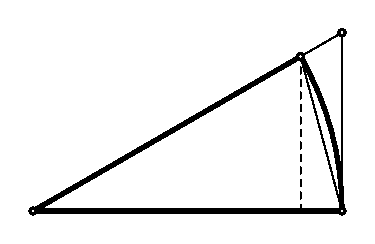
\includegraphics{03dsin.pdf}}
        \put( 15.83,   3.83){\sffamily\itshape $O$}
    \put(164.17,   3.83){\sffamily\itshape $A$}
    \put(161.17, 107.47){\sffamily\itshape $B$}
    \put(141.29,  96.00){\sffamily\itshape $C$}
    \put(157.31,  68.99){\sffamily\itshape $\theta$}
    \put(168.17,  53.65){\sffamily\itshape \rotatebox{90}{$\tan\theta$}}
    \put(134.29,  47.92){\sffamily\itshape \rotatebox{90}{$\sin\theta$}}
\end{picture}
}
  \hspace{0.15\textwidth}
  \begin{minipage}{0.4\textwidth}
    \setlength{\parskip}{1ex plus 1ex}\footnotesize \sffamily
    \raggedright
    \rule{0pt}{16pt}

    The circular wedge $OAC$ contains the triangle $OAC$ and is contained
    in the right triangle $OAB$.

    The area of triangle $OAC$ is $\frac12\sin\theta$.

    The area of circular wedge $OAC$ is $\frac12\theta$.

    The area of right triangle $OAB$ is $\frac12\tan\theta$.

    Hence one has \( \sin\theta < \theta < \tan\theta \) for all angles
    $0<\theta<\pi/2$.  \vspace{10ex}\null
  \end{minipage}
  }
  \caption{Proving $\lim_{\theta\to 0} \dfrac{\sin \theta}{\theta}
    = 1$ by comparing the areas of two triangles and a circular wedge. }
  \label{fig:sintheta-almost-theta}
\end{figure}

\begin{proof}
  The proof requires a few sandwiches and some geometry.  We begin by
  only considering positive angles, and in fact we will only consider
  angles $0<\theta<\pi/2$.

  Look at Figure~\ref{fig:sintheta-almost-theta}.   Since the wedge
  $OAC$ contains the triangle $OAC$ its area must be larger.  The area
  of the wedge is $\frac12\theta$ and the area of the triangle is
  $\frac12\sin \theta$, so we find that
  \begin{equation}\label{eq:03SineBelowTheta}
    0<\sin \theta <\theta \text{ for } 0<\theta<\frac\pi2.
  \end{equation}
  The Sandwich Theorem implies that
  \begin{equation}\label{eq:03limSineisZero}
    \lim_{\theta\searrow 0}\sin\theta = 0.
  \end{equation}
  Moreover, we also have
  \begin{equation}\label{eq:03limCosisOne}
    \lim_{\theta\searrow0}\cos\theta =
    \lim_{\theta\searrow0}\sqrt{1-\sin^2\theta} = 1.
  \end{equation}

  Next we compare the areas of the wedge $OAC$ and the larger triangle
  $OAB$.  Since $OAB$ has area $\frac12\tan \theta$ we find that
  \[
  \theta<\tan\theta
  \]
  for $0<\theta<\frac\pi2$.  Since $\tan\theta =
  \frac{\sin\theta}{\cos\theta}$ we can multiply with $\cos\theta$ and
  divide by $\theta$ to get
  \[
  \cos\theta < \frac{\sin\theta}{\theta} \text{ for }0<\theta<\frac\pi2
  \]
  If we go back to \eqref{eq:03SineBelowTheta} and divide by $\theta$, then we
  get
  \[
  \cos\theta < \frac{\sin\theta}{\theta} < 1
  \]
  The Sandwich Theorem can be used once again, and now it gives
  \[
  \lim_{\theta\searrow0} \frac{\sin\theta}\theta = 1.
  \]
  This is a one-sided limit.  To get the limit in which $\theta\nearrow 0$,
  you use that $\sin\theta$ is an odd function.
\end{proof}

\subsection{The Cosine counterpart of \eqref{eq:03trig-limit}} 
We will show that
\begin{equation}
  \lim_{\theta\to 0}\frac{1-\cos\theta}{\theta^2} = \frac12.
  \label{eq:03CosLimit}
\end{equation}

This follows from $\sin^2\theta+\cos^2\theta=1$.  Namely,
\begin{align*}
  \frac{1-\cos\theta}{\theta^2}
  &= \frac1{1+\cos\theta}\,\frac{1-\cos^2\theta}{\theta^2} \\
  &= \frac1{1+\cos\theta}\,\frac{\sin^2\theta}{\theta^2} \\
  &= \frac1{1+\cos\theta}\left( \frac{\sin\theta}{\theta} \right)^2.
\end{align*}
We have just shown that $\cos\theta\to1$ and $\frac{\sin\theta}\theta \to
1$ as $\theta\to0$, so \eqref{eq:03CosLimit} follows.

This limit claims that for small values of $\theta$ one has
\[
\frac{1-\cos\theta}{\theta^2} \approx \frac{1}{2},
\]
and hence
\[
\cos \theta \approx 1 - \frac{1}{2}\theta^2.
\]


\subsection{The Sine and Cosine of a small angle} 
As promised in  \eqref{eq:03sine-theta-is-roughly-theta}, you can use
the limits in this section to approximate $\sin\theta$ when $\theta$
is small.  Namely, since $\lim_{\theta\to0}\frac{\sin\theta}{\theta} = 1$ it is
reasonable to assume that for small angles $\theta$ one has
$\frac{\sin\theta}{\theta}\approx 1$, or, $\sin\theta \approx \theta$.
Similarly, \eqref{eq:03CosLimit} implies that for small angles
$\theta$ one has $\cos\theta \approx 1 - \frac12\theta^2$.

For instance, to get a quick estimate of $\sin(0.1)$ and $\cos(0.1)$
(where, as always, $0.1$ is measured in radians)
we use \eqref{eq:03sine-theta-is-roughly-theta} and get
\[
\sin 0.1 \approx 0.1, \qquad
\cos 0.1 \approx 1-\tfrac12(0.1)^2 = 0.995.
\]
The formula \eqref{eq:03sine-theta-is-roughly-theta} does not say how
accurate these approximations are.  To see how good the approximations
are you could compare with the actual values of $\sin 0.1$ and $\cos
0.1$.  These are, rounded to six decimals,
\[
\sin 0.1 \approx 0.099\,833,\qquad
\cos 0.1 \approx 0.995\,004.
\]

\subsection{Another example of a removable discontinuity} 
\label{sec:another-example-of-removable-discontinuity}
Since $(\sin x) /x\to1$ as $x\to0$, the function $f(x) = \frac{\sin x}
{x}$ has a removable discontinuity at $x=0$ (see
\S~\ref{sec:removable-discontinuities}.)

\centerline{\input ../figures/221/03sinx-over-x.tex}

\noindent%
The function
\[
f(x) \stackrel{\rm def}=
\begin{cases}
  (\sin x)/x & \text{for }x\neq0,\\
  1 & \text{when }x=0
\end{cases}
\]
is continuous at $x=0$.

\section{Problems} 
\problemfont 
\noindent\itshape
For each of the following limits, either evaluate them \emph{or} show that they
do not exist.  Distinguish between limits which are infinite and limits which do
not exist.\upshape

\begin{multicols}{3}\setlength{\parindent}{0pt}
\problem $\DS \lim_{\theta\to0} \frac{\tan \theta}{\theta}$ 

(Hint: $\tan\theta = \frac{\sin\theta}{\cos \theta}$).
\answer 
the limit is 1.
\endanswer

\problem $\DS \lim_{\theta\to0} \frac{\theta}{\sin \theta}$ 

\answer 
The limit is 1.
Use :
$\frac{\theta}{\sin\theta} = \frac{1}{\frac{\sin\theta}{\theta}}$.
\endanswer

\problem $\DS \lim_{\alpha\to0}\frac{\sin 2\alpha}{\alpha}$ 

(Hint: a substitution)

\problem $\DS \lim_{\alpha\to0}\frac{\sin 2\alpha}{\sin\alpha}$ 

(two ways: with and without the double angle formula!)
\answer 
$\sin 2\alpha = 2\sin\alpha\cos\alpha$ so the limit is
$\lim_{\alpha\to0} \frac{2\sin\alpha\cos\alpha}{\sin\alpha} =
\lim_{\alpha\to0} 2\cos\alpha = 2$.

Other approach: $\DS\frac{\sin2\alpha}{\sin\alpha} =
\frac{\frac{\sin2\alpha}{2\alpha}}{\frac{\sin\alpha}{\alpha}}\cdot
\frac{2\alpha}{\alpha}$. Take the limit and you get 2.
\endanswer

\problem $\DS \lim_{x\to0}\frac{\sin 3x}{2x}$. 

\answer 
$\frac{3}{2}$.
\endanswer



\problem $\DS \lim_{\alpha\to0}\frac{\tan 4\alpha}{\sin 2\alpha}$. 

\answer 
$\frac{\tan 4\alpha}{\sin 2\alpha}
= \frac{\tan 4\alpha}{4\alpha}\cdot
\frac{4\alpha}{2\alpha}\cdot \frac{2\alpha}{\sin2\alpha}$.

Take the limit and you get $\ldots = 1\cdot1\cdot2 = 2$.
\endanswer

\problem $\DS \lim_{x\to 0} \frac{1-\cos x}{ x \sin x}.$ 

\answer 
Hint: multiply top and bottom with \(1+\cos x\).
\endanswer

\problem $\DS\lim_{\theta\to\pi/2}\frac{1-\sin\theta}{\theta-\pi/2}$ 

\answer 
Hint: substitute $\theta = \frac{\pi}{2} - \varphi$, and let $\varphi\to 0$.  Answer: $0$.
\endanswer

\problem $\DS \lim_{x\to0}\frac{\sin^2 x}{1-\cos x}$. 
\answer 
Multiply top and bottom with $1+\cos x$.  The answer is $2$.
\endanswer
\problem $\DS \lim_{x\to0}\frac{\sin(x^2)}{x^2}.$ 
\answer 
Substitute $x^2 = u$ and let $u\to 0$.  Answer: $1$.
\endanswer

\problem $\DS \lim_{x\to 0} \frac{x(1-\cos x)}{ \tan^3 x}.$ 
\answer 
Multiply and divide by $1+\cos x$.  Write $\tan x$ as $\frac{\sin x}{\cos x}$.
Answer is $\frac12$.
\endanswer
\problem $\DS \lim_{x\to 0} \frac{\sin(x^2)}{ 1-\cos x}. $ 
\answer 
$\DS \frac{\sin(x^2)}{ 1-\cos x} = \frac{\sin (x^2)}{x^2} \frac{x^2}{1-\cos x}$.
The answer is $2$.
\endanswer
\problem \(\DS\lim_{x\to\pi/2}\frac{x-\tfrac\pi2}{\cos x}\). 
\answer 
Substitute \(\theta = x-\pi/2\) and remember that \(\cos x = \cos(\theta+\frac\pi2) = -\sin\theta\).  You get
\[
\lim_{x\to\pi/2}\frac{x-\tfrac\pi2}{\cos x} =\lim_{\theta\to0}
\frac{\theta}{-\sin\theta} = -1.
\]
\endanswer

\problem \(\DS\lim_{x\to\pi/2}(x-\tfrac\pi2)\tan x\). 

\answer 
Similar to the previous problem, once you use \(\tan x = \frac{\sin
  x}{\cos x}\). The answer is again \(-1\).
\endanswer

\problem $\DS \lim_{x\to 0}\frac{\cos x}{x^2+9}.$ 
\answer 
$1/9$
\endanswer

\problem $\DS \lim_{x\to \pi}\frac{\sin x}{x-\pi}.$ 

\answer 
Substitute \(\theta = x-\pi\).  Then \(\lim_{x\to\pi}\theta=0\), so
\[
\lim_{x\to \pi}\frac{\sin x}{x-\pi} = \lim_{\theta\to0}
\frac{\sin(\pi+\theta)}{\theta} = -\lim_{\theta\to0}
\frac{\sin\theta}{\theta} = -1.
\]
Here you have to remember from trigonometry that \(\sin(\pi+\theta)
= -\sin\theta\).
\endanswer

\problem $\DS \lim_{x\rightarrow 0}\frac{\sin x}{x+\sin x}.$ 
\answer 
Divide top and bottom by $x$.  The answer is $1/2$.
\endanswer

\problem \carefulnow $\DS A = \lim_{x\to\infty} \frac{\sin x}{x}$. 

\answer 
Note that the limit is for \(x\to\infty\)!  As \(x\) goes to
infinity \(\sin x\) oscillates up and down between \(-1\) and
\(+1\).  Dividing by \(x\) then gives you a quantity which goes to
zero.  To give a good proof you use the Sandwich Theorem like this:
\smallskip

Since \(-1\le \sin x\le 1\) for all \(x\) you have
\[
\frac{-1}{x} \le \frac{\sin x}{x} \le \frac{1}{x}.
\]
Since both \(-1/x\) and \(1/x\) go to zero as \(x\to\infty\) the
function in the middle must also go to zero.  Hence
\[
\lim_{x\to\infty} \frac{\sin x}{x} = 0.
\]
\endanswer

\problem $\DS B = \lim_{x\to\infty} \frac{\cos x}{x}$. 

\answer 
zero again.
\endanswer

\problem \carefulnow $\DS\lim_{x\to\infty} \frac{\tan x}{x}$ 

\problem $\DS\lim_{x\to\infty} \frac{\sin 2x}{x}$ 

\problem $\DS \lim_{x\to\infty} \frac{\sin 2x}{1+x^2}$ 

\problem $\DS \lim_{x\to\infty} \frac{x}{\cos x + x^2}$ 
\answer 
This is not a rational function, but you can use the same trick:  factor out the
highest power of $x$ from numerator and denominator.  You get
\[
 \frac{x}{\cos x + x^2}
 = \frac{x}{x^2} \frac{1}{\frac{\cos x}{x^2} + 1}.
\]
Using the Sandwich Theorem as in the previous problems you get
$\lim_{x\to\infty} \frac{\cos x}{x^2} = 0$.  With the limit properties you then
get
\begin{align*}
  \lim_{x\to\infty}\frac{x}{\cos x + x^2}
 &= \lim_{x\to\infty}\frac{x}{x^2} \frac{1}{\frac{\cos x}{x^2} + 1}\\
 &= 0\times \frac{1}{0+1} \\
 &= 0.
\end{align*}

\endanswer
\problem $\DS \lim_{x\to\infty} \frac{2x^3+3x^2\cos x }{ (x+2)^3}$ 
\answer 
$2$.
\endanswer

\end{multicols}

\begin{multicols}{2}\setlength{\parindent}{0pt}
\problem Since both $\lim_{\theta\to0}\frac{\sin\theta}{\theta} = 1$ and 
$\lim_{\theta\to0}\frac{\tan\theta}{\theta} = 1$, you would think that
for small angles $\theta$
\[
\sin\theta \approx \theta \approx \tan\theta.
\]
In other words the sine and tangent of small angles are almost the
same.  This problem goes into the question of how small the
difference really is.

\subprob Compute $\DS \lim_{\theta\to0}\frac{\tan\theta -
\sin\theta}{\theta^3}$.  

(Hint:  use $\tan\theta = \sin\theta/\cos\theta$.)
\answer 
$\DS \lim_{\theta\to0}\frac{\tan\theta - \sin\theta}{\theta^3} =
\frac{1}{2}$
\endanswer

\subprob  Use your answer from part (a) to estimate the difference
between $\tan 0.1$ and $\sin 0.1$.
\answer 
$\tan0.1 - \sin 0.1 \approx \frac{1}{2}(0.1)^{3} = 0.0005$, which is
really a lot smaller than $0.1$.
\endanswer

\problem Suppose you are lost on an island and you have no calculator. 
Approximate the following quantities as best as you can:

\subprob $\sin{0.2}$
\hfill
\subprob $\cos{0.2}$
\hfill
\subprob $\tan{0.2}$

\subprob $\sin\bigl(\frac\pi2 - {0.2}\bigr)$
\hfill
\subprob $\cos\bigl(\frac\pi2 + {0.2}\bigr)$
\hfill
\subprob $\tan\bigl(\frac\pi2 - {0.2}\bigr)$
\setcounter{SUBPROB}{0}
\answer 
$\sin0.2 \approx 0.2$,

$\cos{0.2} \approx 1-\frac12(0.2)^2 = 0.98$,

$\tan{0.2} = (\sin{0.2})/(\cos{0.2}) \approx 0.2$.

$\sin \bigl(\pi/2 - 0.2\bigr) = \cos 0.2 \approx 0.98$.

$\cos \bigl(\pi/2 + 0.2\bigr) = -\sin 0.2 \approx -0.2$.

$\tan \bigl(\pi/2 - 0.2\bigr) = \dfrac1{\tan 0.2} \approx \dfrac1{0.2} = 50$.

\endanswer
\problem You are still on the island, and you still have no 
calculator.  Approximate the following quantities as best as you can:

\subprob $\sin10^\circ$
\hfill
\subprob $\cos10^\circ$
\hfill
\subprob $\tan10^\circ$


\subprob $\sin100^\circ$
\hfill
\subprob $\cos10^\circ$
\hfill
\subprob $\tan80^\circ$

\carefulnow\ \  Note that here the angles are specified in degrees rather
than radians.

\setcounter{SUBPROB}{0}
\answer 
Same approach as before, but in this problem you first have to convert
$10^\circ$ to radians:
\[
10^\circ = \frac{10}{360}\times2\pi \textrm{radians} = \frac{\pi}{18}.
\]
You get
\[
\sin 10^\circ \approx \frac{\pi}{18},
\]
\[
\cos 10^\circ \approx 1 - \frac{\pi^2}{2\times18^2}.
\]
You don't have a calculator, so, had this been 1965, you would have
enthusiastically computed these numbers by hand (to two decimals).

For a really rough estimate assume $\pi\approx3$, to get
\[
10^\circ \approx \frac{3}{18} = \frac{1}{6} \approx 0.17,
\]
\[
\tan 10^\circ \approx \sin 10^\circ \approx \frac{3}{18} = \frac{1}{6} \approx
0.17,
\]
\begin{align*}
  \cos 10^\circ &\approx 1 - \frac{1}{2} \bigl(\frac{1}{6}\bigr)^2\\
  &= 1- \frac{1}{72}\\
  &\approx 1-0.014 = 0.986
\end{align*}
To find the other expressions, use $\sin(\frac\pi2+\theta) =
\cos\theta$ and $100^\circ = 90^\circ + 10 ^\circ$.

$\sin 100^\circ = \cos10^\circ \approx -0.986 $

$\cos 190^\circ = -\cos 10^\circ \approx -0.986$

$\tan80^\circ = \bigl(\tan 10^\circ\bigr)^{-1} \approx 6$ .
\endanswer

\problem \subprob Simplicio says that while a \textit{million} is clearly a lot, 
\textit{two} is not a large number.  After reading
\eqref{eq:03sine-theta-is-roughly-theta} he then concludes that
\[
\sin(2) \approx 2.
\]
Comment on his conclusion, and explain the meaning of ``small'' in
the sentence ``\textit{if $\theta$ is small then $\sin\theta \approx
\theta$.}''

\subprob The next day Simplicio makes an accurate drawing of a three
degree angle by dividing a right angle ($90^\circ$) into $30$ equal
angles.  The drawing convinces him that three degrees is a very small
angle indeed, and so he concludes that
\[
\sin 3^\circ \approx 3.
\]
Again, comment on Simplicio's reasoning.

\problem Is there a constant $k$ such that the function 
\[
f(x)= \begin{cases}
  \sin(1/x) &\text{for }x\ne 0\\
  k & \text{for } x=0.
\end{cases}
\]
is continuous?  If so, find it; if not, say why no such $k$ exists.
\answer 
No.  As \(x\to0\) the quantity \(\sin \frac{1}{x}\) oscillates
between \(-1\) and \(+1\) and does not converge to any particular
value.  Therefore, no matter how you choose \(k\), it will never be
true that \(\lim_{x\to 0} \sin \frac1x = k\), because the limit
doesn't exist.
\endanswer

\problem Find a constant \(A\) so that the function 
\[
f(x) =
\begin{cases}
  \dfrac{\sin x}{2x} &\hbox{for $x\ne0$} \\
  A & \hbox{when \(x=0\)}
\end{cases}
\]
  is continuous everywhere.
\answer 
The function \(f(x) = (\sin x)/x\) is continuous at all \(x\ne 0\),
so we only have to check that \(\lim_{x\to0} f(x) = f(0)\), i.e.\
\(\lim_{x\to0}\frac{\sin x}{2x} = A\).  This only happens if you
choose \(A=\frac12\).
\endanswer

\problem Compute $\lim_{x\toi}x\sin\frac \pi x$ and $\lim_{x\toi}x 
\tan\frac\pi x$. (Hint: substitute something).


\end{multicols}
\noproblemfont


\section{Asymptotes} 
\label{sec:asymptotes}
Asymptotes can be vaguely defined by saying that a line is an
asymptote of the graph of a function $y=f(x)$ if the graph ``approaches the line
as $x$ approaches infinity.'' For a more precise definition we distinguish
between three cases, depending on the line.

\subsection{Vertical Asymptotes} 
If $y=f(x)$ is a function for which either
\[
\lim_{x\searrow a} f(x) = \infty,
\text{ or }
\lim_{x\searrow a} f(x) = -\infty,
\text{ or }
\lim_{x\nearrow a} f(x) = \infty,
\text{ or }
\lim_{x\nearrow a} f(x) = -\infty
\]
holds, then the line $x=a$ is a \emph{vertical asymptote} of the function $y=f(x)$.

\subsection{Horizontal Asymptotes} 
If $y=f(x)$ is a function for which
\[
\lim_{x\to \infty} f(x) = a \text{ or }
\lim_{x\to-\infty} f(x) = a,
\]then the line $y=a$ is a \emph{horizontal asymptote} of the function
$y=f(x)$.

\subsection{Slanted Asymptotes} 
\label{sec:03slanted-asymptotes}
If $y=f(x)$ is a function for which
\[
\lim_{x\to\infty} \left[ f(x) - \bigl(mx+n\bigr)\right] =0,\text{ or }
\lim_{x\to-\infty} \left[ f(x) - \bigl(mx+n\bigr)\right] =0,
\]
then the line $y=mx+n$ is a \emph{slanted asymptote} for the function
$y=f(x)$.
In this case we say that \emph{the function $f(x)$ is asymptotic to
$mx+n$ as $x\to\infty$} (or $x\to-\infty$, depending on the case).

Slanted asymptotes are the hardest to find, but the following
observations can be helpful.  

\subsection{Asymptotic slope and intercept} 
If $y=mx+n$ is a slanted asymptote of $y=f(x)$ then
\begin{equation}
  m = \lim_{x\to\infty} \frac{f(x)}{x}, \qquad
  n = \lim_{x\to\infty} f(x) - mx.
  \label{eq:03asymptotic-slope-intercept}
\end{equation}
You should be able to prove this yourself. See
problem~\ref{ex:prove-asymptotic-slope-intercept}.
% !!! TO-DO: and conversely, if these two limits exist then the function has y=mx+n as a slant asymptote.

\begin{figure}[bt]
  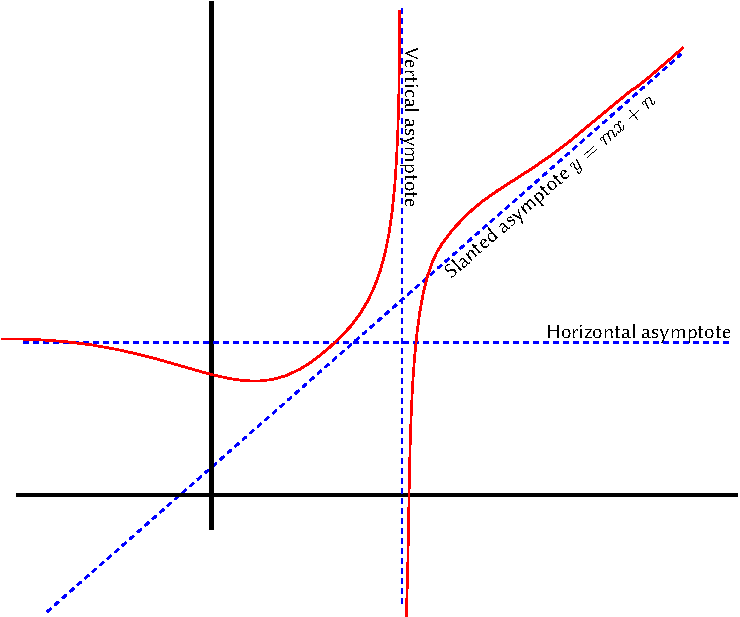
\includegraphics[width=0.6\textwidth]{03asymptotes.pdf}
  \caption{A function with all three kinds of asymptote. }
  \label{fig:03asymptotes}
\end{figure}

\subsection{Example} 
The function
\[
f(x) = \dfrac x{1-x}
\]
has both a horizontal and a vertical asymptote.  To find the
vertical asymptote we look for values of $x$ where the function
``may become infinite.'' The function is well defined everywhere
except when the denominator $1-x$ vanishes.  This happens when $x=1$.
To verify that $x=1$ is a vertical asymptote we compute the limit
\[
\lim_{x\searrow1} f(x) = -\infty \text { and }
\lim_{x\nearrow1} f(x) = +\infty.
\]
Either of these two limits shows that the line $x=1$ is a vertical
asymptote for $y= x/(1-x)$.

To find the horizontal asymptotes we compute
\[
\lim_{x\to\infty} f(x) = -1
\text{ and }
\lim_{x\to-\infty} f(x) = -1.
\]
Again, either of these limits implies that the line $y=-1$ is a
horizontal asymptote for $y=x/(1-x)$.

\subsection{Example} 
Find the asymptotes of the function
\[
f(x) = \sqrt{x^2+1}.
\]
The function is well defined and continuous at all $x$.  This means
that $\lim_{x\to a} f(x)$ is always finite (it's $f(a)$) and therefore
this function has no vertical asymptotes.

Both limits $\lim_{x\to\pm\infty} f(x)$ are infinite so the function
also has no horizontal asymptotes.  

To find possible slanted asymptotes we first see what the slope of
such an asymptote would be:
\[
m
= \lim_{x\to\infty}\frac{f(x)}{x}
= \lim_{x\to\infty}\frac{\sqrt{x^2+1}}{x}
= \lim_{x\to\infty}\sqrt{1+\frac{1}{x^2}} = 1.
\]
This does not yet prove that there is a slanted asymptote; to prove
that one exists we must also find the intercept of the asymptote.
This intercept is given by
\[
n = \lim_{x\to\infty} f(x) - mx
=\lim_{x\to\infty} \sqrt{x^2+1} - x
  = \lim_{x\to\infty} \frac{1}{\sqrt{x^2+1} + x}
  = \lim_{x\to\infty} \frac{1/x}{\sqrt{1+1/x^2} + 1}
  = \dfrac{0}{2}.
\]
This last limit implies that
\[
\lim_{x\to\infty} f(x) - x = 0
\]
and therefore $y=x$ is the slanted asymptote of the function.

\section{Problems} 
\problemfont 
\begin{multicols}{2}
\problem Find the asymptotes (horizontal, vertical and slanted) of the 
following functions:

\subprob $\DS f(x) = \frac{x}{x^2+1}$

\subprob $\DS f(x) = \frac{x}{x^2-4}$

\subprob $\DS f(x) = \frac{5x^2}{x^2-2}$

\subprob $\DS f(x) = \frac{x}{x^2-4}$

\subprob $\DS f(x) = \frac{x}{x-4}$

\subprob $\DS f(x) = \frac{x^3}{x^2+4}$

\problem Which of the following functions have asymptotes? 

\subprob \(\DS f(x) = \sqrt{x} \)
\answer 
No vertical asymptote.  
No horizontal asymptote.  
If there were a slanted asymptote then $m =
\lim_{x\to\infty}\frac{\sqrt{x}}{x} = 0$. But $n = \lim_{x\to\infty}
f(x) - mx = \lim_{x\to\infty}\sqrt{x}$ does not exist.
\endanswer

\subprob \(\DS f(x) = \sqrt{x} - \sqrt{x-1}\)

\subprob \(\DS f(x) = x+ \cos x \)

\subprob \(\DS f(x) = x\sin x \)

\subprob \(\DS f(x) = \dfrac{\sin x}{x} \)

\subprob $\DS f(x) = \sqrt{x^2+x}$

\subprob $\DS f(x) = \frac{x}{\sqrt{x^2+1}}$

\problem Find all asymptotes for the graphs of the following functions: 

\subprob $\DS f(x) = \frac{\sin x}{x^2+4}$

\subprob $\DS f(x) = \frac{\sin x}{x-\pi}$

\subprob $\DS f(x) = \frac{\sin x}{x-1}$

\subprob $\DS f(x) = \tan x$

\subprob $\DS f(x) = \sec \frac x2$

\subprob $\DS f(x) = \arctan x$

\subprob $\DS f(x) = \arctan (x/\pi)$

\subprob $\DS f(x) = \dfrac{\arctan x}{x}$

\subprob $\DS f(x) = \tan \pi x$

\subprob $\DS f(x) = \sec (x^2)$

\problem Give an example of a function $y=f(x)$ that is defined for 
all $x>0$, whose graph has no slanted asymptote, but which still satisfies
\[
\lim_{x\to\infty} \frac{f(x)}{x} = 1.
\]
\problem \textbf{Do a proof!}  Derive the formulas 
\eqref{eq:03asymptotic-slope-intercept}
\label{ex:prove-asymptotic-slope-intercept}
from the definition of slanted asymptote in
\S\ref{sec:03slanted-asymptotes}.

\textit{About finding proofs}:  you can use all the material in this chapter of
the text.  Proofs usually don't ``just come to you.'' Instead they tend to
require some puzzling and most often our first few written attempts at the proof
belong in the trash.  The proof we keep for posterity should be a short and
polished write-up of the argument we find.
\answer 
We are given that
\[
\lim_{x\to\infty} f(x) - mx-n = 0.
\]
Adding $n$ to both sides gives us
\[
\lim_{x\to\infty} f(x) -mx = n,
\]
which is the formula for $n$ we had to prove.

To get the formula for $m$ we multiply with
\[
\lim_{x\to\infty} 1/x =
0
\]
and use the limit properties:
\begin{multline*}
  \lim_{x\to\infty} \frac{f(x)-mx-n}{x} = \\
  \bigl(\lim_{x\to\infty} f(x)-mx-n\bigr)\times
  \bigl(\lim_{x\to\infty}\frac{1}{x}\bigr)=\\
  0\times0 = 0.
\end{multline*}
Work out the left hand side:
\[
0 = \lim_{x\to\infty} \frac{f(x)}{x} - m - \frac{n}{x}.
\]
This implies
\[
0 = \lim_{x\to\infty} \frac{f(x)}{x} - m
\]
and thus
\[
\lim_{x\to\infty} \frac{f(x)}{x} = m.
\]

\endanswer
\problem Suppose the function $y=f(x)$ has exactly one vertical 
asymptote, which happens to be located at $x=1$.  
Which of the following functions have vertical asymptotes, and where
are they located?

\subprob  $g(x) = f(2x)$

\subprob  $h(x) = xf(x)$

\subprob  $h(x) = (x-1)f(x)$

\subprob  $k(x) = f(x)+\sin x$

\end{multicols}
\noproblemfont

%%% Local Variables:
%%% mode: latex
%%% TeX-master: "free221"
%%% End:

% !TEX root = free221.tex

\chapter{Derivatives (2)}




\begin{quote}\itshape
    ``Leibniz never thought of the derivative as a limit''\\[1ex]
  \footnotesize~\hfill
  \href{http://www-history.mcs.st-and.ac.uk/Biographies/Leibniz.html}
  {www-history.mcs.st-and.ac.uk/Biographies/Leibniz.html}\\
\end{quote}




\medskip




\noindent
In Chapter~\ref{ch:derivs1} we saw two mathematical problems which led
to expressions of the form $\frac00$.  Now that we know how to handle
limits, we can state the definition of the derivative of a function.
\marginpar{\footnotesize\sffamily%
  
    \begin{picture} (72.000000,97.666667)(0,0)
    \put(0.0, 0.0){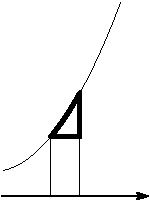
\includegraphics{04derivative-notation-ax.pdf}}
        \put( 24.33,  -4.67){\sffamily\itshape \makebox[0pt][c]{$a$}}
    \put( 36.33,  -4.67){\sffamily\itshape \makebox[0pt][l]{$x$}}
    \put( 40.33,  29.80){\sffamily\itshape \makebox[0pt][l]{$f(a)$}}
    \put( 40.33,  50.80){\sffamily\itshape \makebox[0pt][l]{$f(x)$}}
\end{picture}
\\
  
    \begin{picture} (72.000000,97.666667)(0,0)
    \put(0.0, 0.0){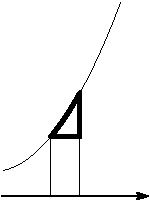
\includegraphics{04derivative-notation-ah.pdf}}
        \put( 24.33,  -4.67){\sffamily\itshape \makebox[0pt][c]{$a$}}
    \put( 36.33,  -4.67){\sffamily\itshape \makebox[0pt][l]{$a+h$}}
    \put( 40.33,  29.80){\sffamily\itshape \makebox[0pt][l]{$f(a)$}}
    \put( 40.33,  50.80){\sffamily\itshape \makebox[0pt][l]{$f(a+h)$}}
\end{picture}
\\
  
    \begin{picture} (72.000000,97.666667)(0,0)
    \put(0.0, 0.0){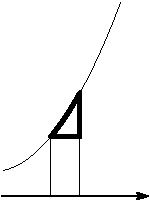
\includegraphics{04derivative-notation-xh.pdf}}
        \put( 24.33,  -4.67){\sffamily\itshape \makebox[0pt][c]{$x$}}
    \put( 36.33,  -4.67){\sffamily\itshape \makebox[0pt][l]{$x+h$}}
    \put( 40.33,  29.80){\sffamily\itshape \makebox[0pt][l]{$f(x)$}}
    \put( 40.33,  50.80){\sffamily\itshape \makebox[0pt][l]{$f(x+h)$}}
\end{picture}
\\
  
    \begin{picture} (72.000000,97.666667)(0,0)
    \put(0.0, 0.0){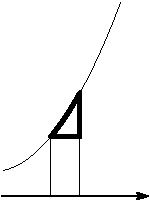
\includegraphics{04derivative-notation-xDx.pdf}}
        \put( 24.33,  -4.67){\sffamily\itshape \makebox[0pt][c]{$x$}}
    \put( 36.33,  -4.67){\sffamily\itshape \makebox[0pt][l]{$x+\Delta x$}}
    \put( 40.33,  29.80){\sffamily\itshape \makebox[0pt][l]{$f(x)$}}
    \put( 40.33,  50.80){\sffamily\itshape \makebox[0pt][l]{$f(x+\Delta x)$}}
\end{picture}
 }%
After computing a few derivatives using the definition we will spend
most of this section developing the \textit{differential calculus,}
which is a collection of rules that allow us to compute derivatives
without always having to use the basic definition.




\section{Derivatives Defined} 
%
\subsection{Definition} 
\label{def:derivative}\itshape
Let $f(x)$ be a function that is defined on an interval $(c, d)$
and let $a$ be a number in this interval.




We say that $f(x)$ is \emph{differentiable at $a$} if the limit
\begin{equation}\label{eq:derivative-defined}
  \lim_{x\to a} \frac{f(x)-f(a)}{x-a}
\end{equation}
exists, and (if it exists) we call the value of the limit the \emph{derivative
of the function $f$ at $a$}, and denote it as $f'(a)$.




\noindent
$f$ is called \emph{differentiable on the interval $(c, d)$} if it is
differentiable at every point $a$ in $(c,d)$.




\upshape




\subsection{Other notations}\label{sec:other-notations} 
We can substitute $x=a+h$ in the limit \eqref{eq:derivative-defined}
and let $h\to0$ instead of $x\to a$.  This gives the formula
\begin{equation}\label{eq:derivative-defined-a-plus-h}
  f'(a) = \lim_{h\to 0} \frac{f(a+h)-f(a)}{h},
\end{equation}
Often this equation is written with $x$ instead of $a$,
\begin{equation}\label{eq:derivative-defined-x-plus-h}
  f'(x) = \lim_{h\to 0} \frac{f(x+h)-f(x)}{h},
\end{equation}
and $\Delta x$ instead of $h$, which makes it look like this:
\begin{equation}\label{eq:derivative-defined-x-plus-Dx}
f'(x) = \lim_{\Delta x\to0} \frac{f(x+\Delta x) - f(x)}{\Delta x}.
\end{equation}
The interpretation is the same as in equation \eqref{eq:difference-quotient}
from \S~\ref{sec:rates-of-change} in Chapter II.  The numerator $f(x+\Delta x) -
f(x)$ represents the amount by which the function value of $f$ changes if we
increase its argument $x$ by a (small) amount $\Delta x$.  If we write $y=f(x)$
then we can call the increase in $f$
\[
\Delta y = f(x+\Delta x) - f(x),
\]
so that the derivative $f'(x)$ is
\[
f'(x) = \lim_{\Delta x\to0}\frac{\Delta y}{\Delta x}.
\]
\textsc{Gottfried Wilhelm von Leibniz}, one of the inventors of calculus,
came up with the idea that one should write this limit as
\[
\frac{dy}{dx}= \lim_{\Delta x\to0}\frac{\Delta y}{\Delta x},
\]
the idea being that after letting $\Delta x$ go to zero it didn't vanish,
but instead became an ``infinitely small quantity'', which Leibniz called
``$dx$''.  The result of increasing $x$ by this ``infinitely small quantity''
$dx$ is that $y=f(x)$ increases by another infinitely small quantity $dy$.
The ratio of these two infinitely small quantities is what we call the
derivative of $y=f(x)$.
\marginpar{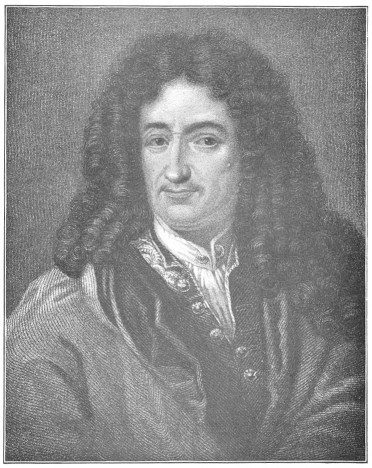
\includegraphics[width=90pt]{Wag_gottfried_wilhelm_leibnitz.jpg}\\
\centering\footnotesize\sffamily%
Leibniz (1646--1716)}




We began the semester by agreeing that there are no ``infinitely small
numbers'', and this makes Leibniz's notation difficult to justify.  In
spite of this we will often use his notation because it shortens
many formulas for derivatives, and it often makes intuitive sense.%
\footnote{So many people use Leibniz' notation that mathematicians have
  tried hard to create a consistent theory of ``infinitesimals'' that
  would allow you to compute with ``$dx$ and $dy$'' as Leibniz and his
  contemporaries would have done.  In the mid 20th century such a
  theory was finally created, and dubbed ``non-standard analysis.'' We
  won't mention it any further, but, as pointed out in a footnote in
  Chapter I, Keisler's calculus text using infinitesimals at\\
  \centerline{\url{http://www.math.wisc.edu/~keisler/calc.html}}\\
  is aimed at undergraduates, so you could have a look if you're
  interested.}


If $f(x)$ is a complicated function, we will often use ``operator notation'' for
the derivative $\dfrac{df}{dx}$, by writing it as
\[
  \frac{d}{dx}\left[f\right].
\]
The symbol $\frac{d}{dx}$ is shorthand for ``take the derivative of what
follows with respect to the variable $x$''.




\section{Direct computation of derivatives} 
\label{sec:direct-derivative-computation}




\subsection{Example -- The derivative of $f(x)= x^2$ is $f'(x) = 2x$  . } 
We have done this computation before in Chapter II,
\S\ref{sec:tangent-to-parabola}.  Using one of our equivalent definitions for the
derivative, say \eqref{eq:derivative-defined-x-plus-Dx}, we get the
same result as before:
\[
f'(x)= \lim_{{\Delta x}\to 0} \frac{f(x+{\Delta x})-f(x)}{{\Delta x}}
= \lim_{{\Delta x}\to 0}
\frac{(x+{\Delta x})^2-x^2}{{\Delta x}}=\lim_{{\Delta x}\to 0} 2x+{\Delta x} =2x.
\]
Leibniz would have written
\[
\frac{dx^2}{dx} = 2x,
\]
and he would have said (in German) that {\slshape ``when you increase
  $x$ by an infinitely small amount $dx$, then $x^2$ will increase by
  the infinitely small amount $2xdx$; hence the ratio between the
  infinitesimal changes in $x^2$ and $x$ is $2x$.''}


  % !!! Leibniz's arguments are not helpful at this stage. Toss them.


\subsection{The derivative of $g(x) = x$ is $g'(x) =1$} 
\label{ex:derivative-of-a-constant}
We'll use the form \eqref{eq:derivative-defined-x-plus-h} of the
definition of the derivative (since writing $h$ is easier than
$\Delta x$'s).  We get:
\[
g'(x)= \lim_{h\to 0} \frac{g(x+h)-g(x)}{h}
= \lim_{h\to 0} \frac{(x+h) -x}{h}=\lim_{h\to 0} \frac{h}{h} =1.
\]
In Leibniz's notation, this says
\[
\frac{d}{dx}\left[x\right] = 1.
\]
This is an example where Leibniz' notation is most persuasive.  In
Leibniz' words, \textit{if you increase $x$ by an infinitely small
  amount $dx$, then the increase of $x$ is of course $dx$, and the
  ratio of these two infinitely small increases is $dx/dx = 1$.}
Sadly, we do not believe in infinitely small numbers, so we cannot
take this explanation seriously.  The expression $\frac{dx}{dx}$ is
not really a fraction since there are no two ``infinitely small''
quantities $dx$ which we are dividing.

\subsection{The derivative of any constant function is zero} 
Let $k(x)=c$ be a constant function.  Then we have
\[
k'(x)= \lim_{h\to 0} \frac{k(x+h)-k(x)}{h}
= \lim_{h\to 0} \frac{c-c}{h}=\lim_{h\to 0} 0 =0.
\]
Leibniz would have said that if $c$ is a constant, then \textit{an
  infinitely small increase $dx$ of the quantity $x$ will not change
  $c$, so the corresponding infinitely small change in $c$ is $dc=0$;
  therefore}
\[
\frac{dc}{dx} = 0.
\]




\subsection{Derivative of $x^n$ for $n=1, 2, 3, \ldots$} 
To differentiate $f(x) = x^n$, it turns out to be easier to use the first
definition \eqref{eq:derivative-defined}.  This definition gives
\[
f'(a) = \lim_{x\to a} \frac{f(x)-f(a)}{x-a} =\lim_{x\to
a}\frac{x^n-a^n}{x-a}.
\]
We need to simplify the fraction $(x^n-a^n)/(x-a)$.
For $n=2$ we have
\[
\frac{x^2-a^2}{x-a} = x+a.
\]
For $n=1, 2, 3, \ldots$ the geometric sum formula tells us that
\begin{equation}
  \label{eq:xn-difference-quotient}
  x^{n-1}+x^{n-2}a+x^{n-3}a^2+\cdots + xa^{n-2}+a^{n-1} =
  \frac{x^n-a^n}{x-a\;}.   
\end{equation}
If you don't remember the geometric sum formula, then you could also just verify
(\ref{eq:xn-difference-quotient}) by carefully multiplying both sides with
$x-a$.  For instance, when $n=3$ you would get
\begin{center}
  \begin{tabular}{r@{}*{8}{c@{}}r}
    $x\cdot(x^2+ax+a^2)$ & $\;=\;$ &
    $x^3$ & $+$ & $ax^2$ & $+$ & $a^2x$ & \\
    $-a\cdot(x^2+ax+a^2)$ & $=$ &
    & $-$ & $ax^2$ & $-$ & $a^2x$ & $-$ & $a^3$ &\hspace{2em}\textit{\small(add)}\\
    \hline
    \rule{0pt}{12pt}
    $(x-a)\cdot(x^2+ax+a^2)$ & $\;=\;$ &  $x^3$ &&&&&$-$&$a^3$
  \end{tabular}
\end{center}
With formula \eqref{eq:xn-difference-quotient} in hand we can now
easily find the derivative of $x^n$:
\begin{align*}
  f'(a)&=\lim_{x\to a}\frac{x^n-a^n}{x-a} \\
  &=\lim_{x\to a}\bigl)
  x^{n-1}+x^{n-2}a+x^{n-3}a^2+\cdots + xa^{n-2}+a^{n-1}\bigr)\\
  &= a^{n-1}+a^{n-2}a+a^{n-3}a^2+\cdots + a\,a^{n-2}+a^{n-1}.
\end{align*}
Here there are $n$ terms, and they all are equal to $a^{n-1}$, so
the final result is
\[
f'(a) = na^{n-1}.
\]
We could also write this as $f'(x) = nx^{n-1}$, or, in Leibniz's
notation
\[
\frac{d}{dx} \left[x^n\right]= nx^{n-1}.
\]
This formula turns out to be true in general, but here we have only
proved it for the case in which $n$ is a positive integer.




\section{Differentiable implies Continuous} 
\subsection{Theorem. } 
\label{sec:04differentiable-implies-continuous}\itshape
If a function $f$ is differentiable at some $a$ in its domain,
then $f $ is also continuous at $a$.
\upshape




\begin{proof}
  We are given that
  \[
  \lim_{x\to a}\frac{f(x)-f(a)}{x-a}
  \]
  exists, and we must show that
  \[
  \lim_{x\to a} f(x) = f(a).
  \]
  This follows from the following computation
  \begin{align*}
    \lim_{x\to a}f(x) &= \lim_{x\to a} \bigl(f(x)-f(a)+f(a) \bigr)
    &\text{(algebra)}\\
    &= \lim_{x\to a} \left(\frac{f(x)-f(a)}{x-a}\cdot(x-a) + f(a)\right)
    &\text{(more algebra)}\\
    &= \left( \lim_{x\to a} \frac{f(x)-f(a)}{x-a}\right) \cdot \lim_{x\to
    a}\left( x-a\right) + \lim_{x\to a} f(a)
    &\text{(Limit Properties)}\\[3pt]
    &= f'(a) \cdot 0 + f(a)
    &(f'(a) \text{ exists})\\[1ex]
    &= f(a).
  \end{align*}
\end{proof}




\section{Some non-differentiable functions} 
\subsection{A graph with a corner. } 
Consider the function
\[
f(x) = |x| =
\begin{cases}
  x&\text{ for $x\geq0$,}\\
  -x & \text{ for $x<0$.}
\end{cases}
\]
This function is continuous at all $x$, but it is not differentiable at $x=0$.




To see this we can try to compute the derivative at 0: we get
\[
f'(0) = \lim_{x\to 0} \frac{|x| - |0|}{x-0}
=\lim_{x\to 0} \frac{|x|}{x}
=\lim_{x\to 0} \sign(x).
\]
But we know this limit does not exist (see~Chapter~III, \S\ref{sec:sign-function-has-no-limit})




\marginpar{\footnotesize\sffamily%
  
    \begin{picture} (90.000000,90.000000)(0,0)
    \put(0.0, 0.0){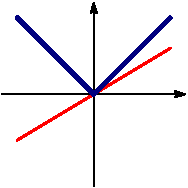
\includegraphics{04absxNoTangent.pdf}}
        \put(  9.33,  17.00){\sffamily\itshape \rotatebox{30.963757}{{\small\sffamily\itshape tangent?}}}
    \put(  8.33,  86.67){\sffamily\itshape \makebox[0pt][c]{$y=|x|$}}
\end{picture}
\\
  The graph of $y=|x|$ has no tangent at the origin}
If we look at the graph of $f(x) = |x|$ then we can see what is wrong:
the graph has a corner at the origin and it is not clear which line,
if any, deserves to be called the tangent line to the graph at the origin.








\subsection{A graph with a cusp. } 
  % !!! Discuss: Change this example to x^{1/3} to make it cleaner?
  Another example of a function without a derivative at $x=0$ is
\[
f(x) = \sqrt{|x|}.
\]%
\marginpar{\footnotesize\sffamily%
  
    \begin{picture} (90.000000,79.000000)(0,0)
    \put(0.0, 0.0){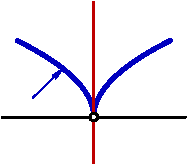
\includegraphics{04sqrtNoTangent.pdf}}
        \put(  1.00,  27.00){\sffamily\itshape $y=\surd{|x|}$}
    \put( 37.00,  48.67){\sffamily\itshape \rotatebox{90}{\small\sffamily\itshape tangent? }}
\end{picture}
\\
  The tangent to the graph of $y=|x|^{1/2}$ at the origin is vertical,
  so its slope is not defined.  The origin is the only
  point on the graph of $y=|x|^{1/2}$ where the tangent is vertical.}%
When you try to compute the derivative you get this limit
\[
f'(0) = \lim_{x\to0} \frac{\sqrt{|x|}}{x} = \text{?}
\]
The limit from the right is
\[
\lim_{x\searrow 0} \frac{\sqrt{|x|}}{x}
= \lim_{x\searrow 0} \frac1{\sqrt x},
\]
which does not exist (it is ``$+\infty$'').  Likewise, the limit from
the left also does not exist (it's ``$-\infty$'').  Nonetheless, a
drawing for the graph of $f$ suggests an obvious tangent line to the graph
at $x=0$, namely the $y$-axis.  That observation does not give us a
derivative, because the $y$-axis is vertical and its slope is not defined.

\begin{figure}
  
    \begin{picture} (360.000000,128.408424)(0,0)
    \put(0.0, 0.0){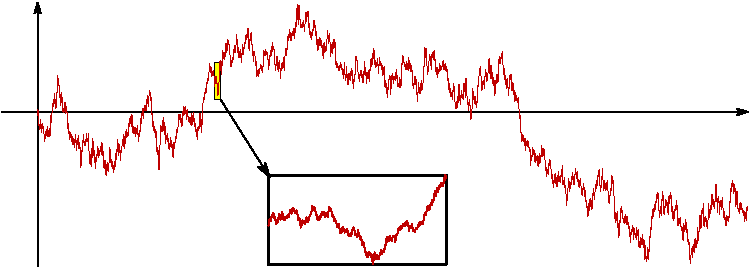
\includegraphics{04brownianMo.pdf}}
        \put(118.14,  64.03){\sffamily\itshape \makebox[0pt][l]{{\rmfamily\itshape\footnotesize(magnify)}}}
    \put(354.74,  78.92){\sffamily\itshape $t$}
    \put( 23.05, 122.29){\sffamily\itshape $x(t)$}
\end{picture}

  \caption{A ``Brownian motion'' provides an example of a function
    $y=f(x)$ that is not differentiable at any $x$.  The graph
    looks like it zig-zags up and down everywhere.  If you magnify any
    small piece of the graph it still has the same jagged appearance. }
\end{figure}

\subsection{A graph with absolutely no tangents, \emph{anywhere}. } 
The previous two examples were about functions that did not have a
derivative at $x=0$.  In both examples the point $x=0$ was the only point
where the function failed to have a derivative.  It is easy to give
examples of functions that are not differentiable at more than one value of
$x$, but here I would like to show you a function $f$ that doesn't have a
derivative \emph{anywhere in its domain.  }

To keep things short I won't write a formula for the function, and merely show
you a graph.  In this graph you see a typical path of a Brownian motion, i.e.\
$t$ is time, and $x(t)$ is the position of a particle which undergoes a Brownian
motion -- come to lecture for further explanation (see also the article on
wikipedia).  To see a similar graph check the Dow~Jones, Nasdaq or S\&P~500 at
the top of the page at \url{http://finance.yahoo.com} in the afternoon on any
weekday.
%\footnote{or at \url{https://www.google.com/finance?client=ob&q=INDEXDJX:DJI}}
% this link is broken
% bummer.


\section{Problems} 
\problemfont 

\begin{multicols}{2}\setlength{\parindent}{0pt}
\noindent%
Compute the derivatives of the following functions,
using either \eqref{eq:derivative-defined} or
\eqref{eq:derivative-defined-a-plus-h}.

\problem $f(x) = x^2-2x $. 
\problem $g(x) = \frac1x $. 
\problem $k(x) = x^3-17x $. 
\problem $u(r) = \frac2{1+r} $. 
\problem $v(\theta) = \sqrt{\theta} $. 
\problem $\varphi(m) = 1/{\sqrt m}$. 
\problem $f(t) = \sqrt[3]{t}$ 
\problem $f(t) = \sqrt{1+2t}$ 
\problem $f(x) = 1/x^2$ 
\problem $f(x) = \sqrt{1+2x} + 1/x^2$ 




\problem Which of the following functions is differentiable at $x=0$? 
\begin{align*}
  f(x) &= x|x|, &g(x) &= x\sqrt{|x|}, \\
  h(x) &= x+|x|, &k(x) &= x^2\sin\frac\pi x,\\
  \ell(x) &= x\sin\frac\pi x.&&
\end{align*}
These formulas do not define $k$ and $\ell$ at $x=0$.  We define $k(0) =
\ell(0) = 0$.

\problem For which value(s) of $a$ and $b$ is the function defined by 
\[
f(x) = \begin{cases}
  ax+b &\text{for $x<0$} \\
  x-x^2 & \text{for $x\geq 0$}
\end{cases}
\]
differentiable at $x=0$?  Sketch the graph of the function $f$ for the
values of $a$ and $b$ you found.

\problem For which value(s) of $a$ and $b$ is the function defined by 
\[
f(x) = \begin{cases}
  ax^2+b &\text{for $x<1$} \\
  x-x^2 & \text{for $x\geq 1$}
\end{cases}
\]
differentiable at $x=1$?  Sketch the graph of the function $f$ for the
values of $a$ and $b$ you found.

\problem For which value(s) of $a$ and $b$ is the function defined by 
\[
f(x) = \begin{cases}
  ax^2 &\text{for $x<2$} \\
  x +b& \text{for $x\geq 2$}
\end{cases}
\]
differentiable at $x=2$?  Sketch the graph of the function $f$ for the
values of $a$ and $b$ you found.

\problem \groupproblem 
\textit{True or false? } If a function $f$ is continuous at some $x=a$
then it must also be differentiable at $x=a$.

\problem \groupproblem 
\textit{True or false? } If a function $f$ is differentiable at some
$x=a$ then it must also be continuous at $x=a$.




\end{multicols}




\noproblemfont
\section{The Differentiation Rules} 
We could go on and compute more derivatives from the definition.  But each time, we
would have to compute a new limit, and hope that there is some trick that allows
us to find that limit.  This is fortunately not necessary.  It turns out that
if we know a few basic derivatives (such as $dx^n/dx=nx^{n-1}$) then we can
find derivatives of arbitrarily complicated functions by breaking them into
smaller pieces.  In this section we look at rules telling us how to
differentiate any function written as either the sum, difference, product or
quotient of two other functions.




\begin{table}[b]
  \centering
  \begin{tabular}[b]
    {l@{\hspace{24pt}}r@{$\,=\,$}l
      @{\hspace{24pt}}r@{$\,=\,$}l}
    \toprule
    \textit{Constant Rule: } & $c'$&$0$ &$\dfrac{dc}{dx}$&$0$ \\[2ex]
%%
    \textit{Sum Rule: } &$(f\pm g)'$&$f'\pm g'$
    &$\dfrac{d}{dx}(f\pm g)$ &$\dfrac{df}{dx}\pm\dfrac{dg}{dx}$ \\[2ex]
%%
    \textit{Product Rule: }
    &$(f\cdot g)'$&$f'\cdot g+f\cdot g'$
    &$\dfrac{d}{dx}(f\cdot g)$ &$\dfrac{df}{dx}\cdot g+f\cdot\dfrac{dg}{dx}$ \\[2ex]
%%
    \textit{Quotient Rule: }
    &$\left(\dfrac{f}{g}\right)'$&$\dfrac{f'\cdot g-f\cdot g'}{g^2}$
    &$\dfrac{d}{dx}\left(\dfrac{f}{g}\right)$
    &$\dfrac{\frac{df}{dx}\cdot g-f\cdot\frac{dg}{dx}}{g^2}$\\[6pt]
    \bottomrule
  \end{tabular}
  \smallskip




  \caption{The differentiation rules:  if you know the derivatives of
    two functions $u(x)$ and $v(x)$, then these rules tell you what
    the derivatives of their sum, product and quotient are.}
  \label{fig:diff-rules}
\end{table}

The situation is analogous to that of the ``limit properties''
$(P_1)$--$(P_6)$ from the previous chapter which allowed us to
compute limits without always having to go back to the formal
definition.

\subsection{Sum, Product, and Quotient Rules} 
In the following, $c$ and
$n$ are constants, $f$ and $g$ are functions of $x$, and ${}'$ denotes
differentiation. The differentiation rules in function notation, and
Leibniz notation, are listed in Table~\ref{fig:diff-rules}.


Note that we already proved the Constant Rule in
\S~\ref{ex:derivative-of-a-constant}.  We will now prove the Sum,
Product and Quotient Rules.

\subsection{Proof of the Sum Rule} 
Suppose that $h(x)=f(x)+g(x)$ for
all $x$ where $f$ and $g$ are differentiable. Then
\begin{align*}
  h'(a)
  & =\lim_{x\to a}\frac{h(x)-h(a)}{x-a}
  &&\textsf{(definition of $h'$)} \\
  & =\lim_{x\to a}\frac{\bigl(f(x)+g(x)\bigr)-\bigl(f(a)+g(a)\bigr)}{x-a}
  &&(\textsf{use }h=f+g)\\
  & =\lim_{x\to a}\left(\frac{f(x)-f(a)}{x-a}+\frac{g(x)-g(a)}{x-a}\right)
  &&\textsf{(algebra)} \\
  & =\left(\lim_{x\to a}\frac{f(x)-f(a)}{x-a}\right)+\left(\lim_{x\to a}\frac{g(x)-g(a)}{x-a}\right)
  &&\textsf{(limit property)} \\[3pt]
  &=f'(a)+g'(a).
  &&\textsf{(definition of $f'$, $g'$)}
\end{align*}






\subsection{Proof of the Product Rule} 
The Product Rule is strange, at
first sight.  In fact, Leibniz first thought that it should look more
like the Sum Rule, and that $(fg)'$ should equal $f'\,g'$.  After
a while he discovered his mistake and figured out that $(fg)' =f'\,g+f\, g'$.  Below is a proof that this rule is correct.  There is
also a picture proof, which we get around to in
\S~\ref{sec:picture-product-rule}.

Let $h(x) = f(x)g(x)$.  To find the derivative we must express the
change of $h$ in terms of the changes of $f$ and $g$:
\begin{align*}
  h(x)-h(a) &= f(x)g(x)-f(a)f(a) \\
  &= f(x)g(x)\underbrace{-f(x)g(a)+f(x)g(a)}_{%
    \makebox[0pt]{\footnotesize\sffamily\centering%
      add and subtract the same term}}
    -f(a)g(a)\\
  &=f(x)\bigl(f(x)-g(a)\bigr) + \bigl(f(x)-g(a)\bigr)v(a)
\end{align*}   
Now divide by $x-a$ and let $x\to a$:
\begin{align*}
  \lim_{x\to a} \frac{h(x)-h(a)}{x-a}
  &= \lim_{x\to a} f(x) \frac{g(x)-g(a)}{x-a} +
  \frac{f(x)-f(a)}{x-a} g(a) \\[1ex]
%  &= \Bigl(\lim_{x\to a} u(x) \Bigr)
%  \Bigl(\lim_{x\to a}\frac{v(x)-v(a)}{x-a} \Bigr)
%  + \Bigl(\lim_{x\to a}\frac{u(x)-u(a)}{x-a} \Bigr)v(a)\\
  &= f(a)g'(a) + f'(a)g(a),
\end{align*}
as claimed.  In this last step we have used that
\[
\lim_{x\to a}\frac{f(x)-f(a)}{x-a} = f'(a)
\quad\text{and}\quad
\lim_{x\to a}\frac{g(x)-g(a)}{x-a} = g'(a)
\]
and also that
\[
\lim_{x\to a} f(x) = u(a)
\]
This last limit follows from the fact that $u$ is continuous,
which in turn follows from the fact that $u$ is differentiable.




  
\subsection{Proof of the Quotient Rule} \label{sec:proof-of-quotient-rule} 
We can break the proof into two parts.  First we do the special case
where $h(x) = 1/g(x)$, and then we use the Product Rule to
differentiate
\[
q(x) = \frac{f(x)}{g(x)} = f(x)\cdot\frac1{g(x)}\;.
\]
So let $h(x) = 1/g(x)$.  We can express the change in $h$ in terms of
the change in $g$:
\[
h(x)-h(a) = \frac1{g(x)} - \frac1{g(a)}
=\frac{g(x)-g(a)}{g(x)g(a)}.
\]
Dividing by $x-a$, we get
\[
\frac{h(x)-h(a)}{x-a} = \frac1{g(x)g(a)} \frac{g(x)- g(a)}{x-a}.
\]
Now we want to take the limit $x\to a$.  We are given that $g$ is
differentiable so it must also be continuous and hence
\[
\lim_{x\to a}g(x) = g(a).
\]
Therefore we find
\[
\lim_{x\to a} \frac{h(x)-h(a)}{x-a} =
\lim_{x\to a}\frac1{g(x)g(a)} \;\lim_{x\to a} \frac{g(x)- g(a)}{x-a}
=\frac{g'(a)}{g(a)^2}.
\]
That completes the first step of the proof.  In the second step,
we use the Product Rule to differentiate $q=f/g$:
\[
q' = \left( \frac fg \right)'
  =\left( f\cdot \frac{1}{g} \right)'
  =f'\cdot\frac{1}{g} + f\cdot\left(  \frac{1}{g}\right)'
=\frac{f'}g - f\frac{g'}{g^2}
=\frac{f'g -fg'}{g^2}.
\]












\subsection{A shorter, but not quite perfect derivation of the Quotient Rule} 
The Quotient Rule can be derived from the Product Rule as follows: for $q=f/g$ then
\begin{equation}\label{eq:quotient-implicity-defined}
  q\cdot g=f
\end{equation}
By the Product Rule, we have
\[
q'\cdot g+q\cdot g'=f',
\]
so that
\[
q' = \frac{f'-q\cdot g'}{g}
= \frac{f'-(f/g)\cdot g'}{g}
=\frac{f'\cdot g-f\cdot g'}{g^2}.
\]
Unlike the proof in \S\ref{sec:proof-of-quotient-rule} above, this argument does
  not prove that $q$ is differentiable if $f$ and $g$ are.
It only says that \emph{if the derivative exists} then it must be what the
Quotient Rule says it is.




The trick we have used here is a special case of a method called ``implicit
differentiation'', which we will discuss much more in
\S~\ref{sec:implicit-differentiation}.




\subsection{Differentiating a constant multiple of a function} 
\label{par:derivative-of-constant-multiple}
Note that the rule
\[
(cf)'=c\,f'
\quad\text{or}\quad
\frac{d\,cu} {dx} = c\, \frac{du} {dx}
\quad\text{or}\quad
\frac{d}{dx}(cf) = c\, \frac{df} {dx}
\]
follows from the Constant Rule and the Product Rule.




\subsection{Picture of the Product Rule} 
  % To write this with f and g instead of u and v, the diagram needs to change
  % in this section.
\label{sec:picture-product-rule}
If $u$ and $v$ are quantities that depend on $x$, and if increasing $x$ by
$\Delta x$ causes $u$ and $v$ to change by $\Delta u$ and $\Delta v$, then the
product of $u$ and $v$ will change by
\begin{equation}
  \label{eq:Delta-uv}
  \Delta(uv)
  =(u+\Delta u)(v+\Delta v) - uv
  = u\Delta v+v\Delta u + \Delta u \Delta v.
\end{equation}
If $u$ and $v$ are differentiable functions of $x$, then the changes $\Delta u$
and $\Delta v$ will be of the same order of magnitude as $\Delta x$, and thus
one expects $\Delta u\Delta v$ to be much smaller.  One therefore ignores the
last term in \eqref{eq:Delta-uv}, and thus arrives at
\[
\Delta(uv) =  u\Delta v+v\Delta u.
\]
Leibniz would now divide by $\Delta x$ and replace $\Delta$'s by $d$'s
to get the Product Rule:
\[
\frac{\Delta(uv)}{\Delta x}
=  u\frac{\Delta v}{\Delta x}+v\frac{\Delta u}{\Delta x}.
\]
\begin{figure}[h]\centering
  
    \begin{picture} (200.000000,158.750000)(0,0)
    \put(0.0, 0.0){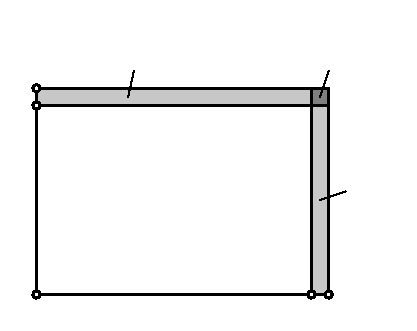
\includegraphics{04prodRulePicture.pdf}}
        \put( 83.50,   5.50){\sffamily\itshape \makebox[0pt][c]{$u$}}
    \put(153.62,   5.50){\sffamily\itshape \makebox[0pt][c]{$\Delta u$}}
    \put( 14.50,  62.87){\sffamily\itshape \makebox[0pt][r]{$v$}}
    \put( 14.50, 112.37){\sffamily\itshape \makebox[0pt][r]{$\Delta v$}}
    \put( 83.50,  62.87){\sffamily\itshape \makebox[0pt][c]{$uv$}}
    \put(168.00,  67.00){\sffamily\itshape \makebox[0pt][l]{$v\Delta u$}}
    \put( 64.25, 126.75){\sffamily\itshape \makebox[0pt][c]{$u\Delta v$}}
    \put(157.75, 126.75){\sffamily\itshape \makebox[0pt][c]{$\Delta u\Delta v$}}
\end{picture}

  \caption{The Product Rule. \textit{How much does the area of a rectangle
  change if its sides $u$ and $v$ are increased by $\Delta u$ and
  $\Delta v$? } Most of the increase is accounted for by the two thin
  rectangles whose areas are $u\Delta v$ and $v\Delta u$.  So the increase
  in area is approximately $u\Delta v + v\Delta u$, which explains why the
  product rule says $(uv)' = uv'+ vu'$. }
\end{figure}




\section{Differentiating powers of functions} 
% !!! Evan did not bother fixing typos here since he wants to delete this entire section, for being just special cases of the chain rule
\subsection{Product rule with more than one factor} 
If a function is given as the product of $n$ functions, i.e.
\[
f(x) = u_1(x) \times u_2(x) \times \cdots \times  u_n(x),
\]
then you can differentiate it by applying the product rule $n-1$ times
(there are $n$ factors, so there are $n-1$ multiplications.)




In the first step you write $f(x)$ as the product of two functions
\[
f(x) = u_1(x) \times \bigl(u_2(x)u_3(x)\cdots u_n(x)\bigr),
\]
would get
\[
f' = u_1' \bigl(u_2\cdots u_n\bigr) + u_1\bigl(u_2\cdots u_n\bigr)'.
\]
In the second step you apply the product rule to $(u_2u_3\cdots
u_n)'$.  This yields
\begin{align*}
  f'
  &= u_1' u_2\cdots u_n + u_1\bigl[u_2'u_3\cdots u_n+u_2(u_3\cdots
  u_n)'\bigr]\\
  &= u_1'u_2\cdots u_n + u_1u_2'u_3\cdots u_n + u_1u_2\bigl(u_3\cdots
  u_n\bigr)'.
\end{align*}
Continuing this way one finds after $n-1$ applications of the product rule
that
\begin{equation}
  \label{eq:product-rule-n-factors}
  \bigl(u_1\cdots u_n\bigr)'
  = u_1'u_2\cdots u_n + u_1u_2'u_3\cdots u_n +\, \cdots\, + u_1u_2u_3\cdots
  u_n'.
\end{equation}








\subsection{The Power rule} 
  % !!! Discuss: delete this section too
If all $n$ factors in the previous paragraph are the same, i.e.\ $u_1(x) =
u_2(x) = \cdots = u_n(x) = u(x)$, then the function $f$ is the
$n^{\text{th}}$ power of some other function,
\[
f(x) = \bigl(u(x)\bigr)^n.
\]
If we use the product rule to find the derivative of $f(x)$, we find that
all terms in the right hand side of \eqref{eq:product-rule-n-factors} are
the same.  Since there are $n$ of them, we get
\[
f'(x) = n\, u(x)^{n-1}\, u'(x),
\]
or, in Leibniz' notation,
\begin{equation}
  \label{eq:Power-rule}
  \frac{du^n}{dx} = nu^{n-1}\frac{du}{dx}.
\end{equation}












\subsection{The Power Rule for Negative Integer Exponents} 
    % !!! Discuss: move this to where the power rule is initially discussed and
    % simply say that the negative exponent case also holds, but without
    % providing a proof there.
We have just proved the power rule \eqref{eq:Power-rule} assuming $n$ is a
positive integer.  The rule actually holds for all real exponents $n$, but
the proof is harder.  




Here we prove the Power Rule for negative exponents using the Quotient
Rule.  Suppose $n=-m$ where $m$ is a positive integer.   Then the Quotient
Rule tells us that
\[
(u^n)'
=\bigl(u^{-m}\bigr)'
=\left(\frac{1}{u^m}\right)'
\stackrel{\text{Q.R.}}{=}
-\frac{(u^m)'}{(u^m)^2}.
\]
Since $m$ is a positive integer, we can use \eqref{eq:Power-rule}, so
$(u^m)' = mu^{m-1}$, and hence
\[
(u^n)'
= -\frac{mu^{m-1}\cdot u'}{u^{2m}}
=-mu^{-m-1}\cdot u'
= n u^{n-1}u'.
\]








\subsection{The Power Rule for Rational Exponents} 
      % !!! Discuss: move this to where the power rule is initially discussed and simply say that the negative exponent case also holds, but without providing a proof there.
      % !!! Issue: this application of implicit differentiation is totally bogus
      % (without having covered implicit differentiation yet).
So far we have proved that the power law holds if the exponent $n$ is an
integer.




We now show that the power law holds even if the exponent $n$ is any
fraction, $n=p/q$.  The following derivation contains the trick called
\emph{implicit differentiation} which we will study in more detail in
Section~\ref{sec:implicit-differentiation}.




So let $n=p/q$ where $p$ and $q$ are integers and consider the function
\[
w(x)=u(x)^{p/q}.
\]
Assuming that both $u$ and $w$ are differentiable functions, we will show that
\begin{equation}\label{eq:power-rule-rational-exponents}
  w'(x) = \frac pq u(x)^{\frac pq-1}u'(x)
\end{equation}








Raising both sides to the $q$th power gives
\[
w(x)^q=u(x)^p.
\]
Here the exponents $p$ and $q$ are integers, so we may apply the Power Rule
to both sides.  We get
\[
qw^{q-1}\cdot w'=pu^{p-1}\cdot u'.
\]
Dividing both sides by $qw^{q-1}$ and substituting $u^{p/q}$ for $w$ gives
\[
w'= \frac{pu^{p-1}\cdot u'}{qw^{q-1}}=
\frac{pu^{p-1}\cdot u'}{qu^{p(q-1)/q}}=
\frac{pu^{p-1}\cdot u'}{qu^{p-(p/q)}}=
\frac{p}{q}\cdot u^{(p/q)-1}\cdot u'
\]
which is the Power Rule for $n=p/q$.

This proof is flawed because we did not show that $w(x) = u(x)^{p/q}$ is
differentiable:  we only showed what the derivative should be,
\textit{if it exists. }

\subsection{Derivative of $x^n$ for integer $n$} 
  % This is beyond pointless to include here!!!
If you choose the function $u(x)$ in the Power Rule to be $u(x) = x$, then
$u'(x) = 1$, and hence the derivative of $f(x) = u(x)^n = x^n$ is
\[
f'(x)
= nu(x)^{n-1} u'(x)
= nx^{n-1}\cdot 1
= nx^{n-1}.
\]
We already knew this of course.

\subsection{Example -- differentiate a polynomial} 
Using the Differentiation Rules we can easily differentiate any polynomial and
hence any rational function.  For example, using the Sum Rule, the Power Rule,
and the rule $(cu)'=cu'$, we see that the derivative of the polynomial
\[
f(x)= 2x^4-x^3+7
\]
is
\[
f'(x)=8x^3-3x^2.
\]

\subsection{Example -- differentiate a rational function} 
By the Quotient Rule the derivative of the function
\[
g(x)=\frac{2x^4-x^3+7}{1+x^2}
\]
is
\begin{align*}
  g'(x)&=\frac{(8x^3-3x^2)(1+x^2)-(2x^4-x^3+7)2x}{(1+x^2)^2}\\
  &=\frac{6x^5-x^4+8x^3-3x^2-14x}{(1+x^2)^2}.
\end{align*}
By comparing this example with the previous one, it seems to be the case that
polynomials simplify when we differentiate them, while rational
functions become more complicated.

\subsection{Derivative of the square root} 
The derivative of $f(x)=\sqrt{x}=x^{1/2}$ is
\[
f'(x)
= \frac12 x^{1/2 -1}
= \frac12 x^{-1/2}
= \frac1{2x^{1/2}}=\frac1{2\sqrt x}
\]
where we used the Power Rule with $n=1/2$ and $u(x)=x$.

\section{Problems} 
\problemfont 
\begin{multicols}{2}\setlength{\parindent}{0pt}
\problem Let $f(x)=(x^2+1)(x^3+3)$. Find $f'(x)$ in two ways:\\ 
\textbf{(a)}~by multiplying and then differentiating, \\
\textbf{(b)}~by using the Product Rule.\\
Are your answers the same?


\problem  Let $f(x)=(1+x^2)^4$. Find $f'(x)$ in two ways, first by 
expanding to get an expression for $f(x)$ as a polynomial in $x$ and
then differentiating, and then by using the Power Rule.  Are the
answers the same?

\problem Prove the statement in \S\ref{par:derivative-of-constant-multiple}, that $(cu)' = c(u')$ follows from the Product Rule. 








\noindent \textit{Compute the derivatives of the following functions}
(Try to simplify your answers.)\\




\problem $\DS f(x) = x+1+(x+1)^2$ 




\problem $\DS f(x) = \frac{x-2}{x^4+1}$ 




\problem $\DS f(x) = \left(\frac{1}{1+x}\right)^{-1}$ 




\problem $\DS f(x) = \sqrt{1-x^2}$ 




\problem $\DS f(x) = \frac{ax+b}{cx+d}$ 




\problem $\DS f(x) = \frac1{(1+x^2)^2}$ 




\problem $\DS f(x) = \frac{x}{1+\sqrt x}$ 




\problem $\DS f(x) = \sqrt{\frac{1-x}{1+x}}$ 




\problem $\DS f(x) = \sqrt[3]{x+\sqrt x}$ 




\problem $\DS \varphi(t) = \frac{t}{1+\sqrt t} $ 




\problem $\DS g(s) = \sqrt{\frac{1-s}{1+s}} $ 




\problem $\DS h(\rho) = \sqrt[3]{\rho+\sqrt \rho}$ 












\problem \groupproblem\textit{Using derivatives to approximate numbers. } 




\subprob Find the derivative of $f(x) = x^{4/3}$.




\subprob Use \textbf{(a)} to estimate the number
\[
\frac{127^{4/3}-125^{4/3}}{2}
\]
approximately without a calculator. Your answer should have the form
$p/q$ where $p$ and $q$ are integers.  [\textsl{Hint: Note that
$5^3=125$ and take
a good look at equation \eqref{eq:derivative-defined}.}]




\subprob Approximate in the same way the numbers $\sqrt{99}$ and
$\sqrt{101}$. (Hint: $10\times 10=100$.)








\problem\label{ex:05log-derivs} 
  % This problem shouldn't be here, it should be later with logs and exponentials!
\textit{(Making the Product and Quotient rules look nicer)}




Instead of looking at the derivative of a function you
can look at the ratio of its derivative to the function itself, i.e.\
you can compute $f'/f$.  This quantity is called the
\emph{logarithmic derivative of the function $f$} for reasons that
will become clear later this semester.
% add forward reference to logs section


\subprob Compute the logarithmic derivative of these functions (i.e., find
$f'(x)/f(x)$):
\begin{gather*}
  f(x) = x ,\quad g(x) =3x ,\\
  h(x) =x^2 \quad k(x) =-x^2 ,\\
  \ell(x) =2007x^2,\quad m(x) =x^{2007}
\end{gather*}




\subprob Show that for any pair of functions $u$ and $v$ one has
\begin{align*}
  \frac{(uv)'}{uv} &= \frac{u'}{u} + \frac{v'}{v}\\
  \frac{(u/v)'}{u/v} &= \frac{u'}{u} - \frac{v'}{v}\\
  \frac{\bigl(u^n\bigr)'}{u^n} &= n\; \frac{u'}{u}
\end{align*}
















\problem   
\subprob Find $f'(x)$ and $g'(x)$ if
\[
f(x)=\frac{1+x^2}{2x^4+7}, \qquad g(x)=\frac{2x^4+7}{1+x^2}.
\]
Note that $f(x)=1/g(x)$.\\
\subprob Is it true that $f'(x)=1/g'(x)$?\\
\subprob Is it true that $f(x) = g^{-1}(x)$?\\
\subprob Is it true that $f(x)= g(x)^{-1}$?\\








\problem \subprob Let 
\begin{gather*}
  x(t)=(1-t^2)/(1+t^2),\\
  y(t)=2t/(1+t^2),\\
  u(t)=y(t)/x(t).
\end{gather*}
Find $dx/dt$, $dy/dt$.




\subprob Now that you've done \textbf{(a)} there are two
different ways of finding $du/dt$.  Do
both of them, and compare the results you get.




\end{multicols}
\normalsize\rmfamily








\noproblemfont
\section{Higher Derivatives} 




\subsection{The derivative of a function is a function} 
If the derivative $f'(a)$ of some function $f$ exists for all $a$ in the domain
of $f$, then we have a new function: namely, for each number in the domain of
$f$ we compute the derivative of $f$ at that number.  This function is called
the \emph{derivative function} of $f$, and it is denoted by $f'$.  Now that we
have agreed that the derivative of a function is a function, we can repeat the
process and try to differentiate the derivative.  The result, if it exists, is
called the \emph{second derivative of $f$}.  It is denoted $f''$.  The
derivative of the second derivative is called the third derivative, written
$f'''$, and so on.




The $n$th derivative of $f$ is denoted $f^{(n)}$.  Thus
\[
f^{(0)}=f,\qquad f^{(1)}=f',\qquad f^{(2)}=f'',\qquad
f^{(3)}=f''',\ldots.
\]
Leibniz' notation for the $n$th derivative of $y=f(x)$ is
\[
\frac{d^ny}{dx^n}= f^{(n)}(x).
\]








\subsection{Two examples} 
If $f(x) = x^2-2x+3$ and $g(x) = x/(1-x)$ then
\begin{align*}
  f(x) &= x^2 - 2x + 3  & g(x)&= \frac{x} {1-x} \\
  f'(x) &= 2x -2 & g'(x) &= \frac{1} {(1-x)^2} \\
  f''(x) &= 2 & g''(x) &= \frac{2} {(1-x)^3} \\
  f^{(3)}(x) &= 0 & g^{(3)}(x) &= \frac{2\cdot 3} {(1-x)^4}\\
  f^{(4)}(x) &= 0 & g^{(4)}(x) &= \frac{2\cdot3\cdot4} {(1-x)^5}\\
  &\vdots &&\vdots
\end{align*}
All further derivatives of $f$ are zero, but no matter how often we
differentiate $g(x)$ we will never get zero.  Instead of multiplying the
numbers in the numerator of the derivatives of $g$ we left them as
``$2\cdot3\cdot4$.''  A good reason for doing this is that we can see
a pattern in the derivatives, which would allow us to guess what (say) the
$10$th derivative is, without actually computing ten derivatives:
\[
g^{(10)}(x) =
\frac{2\cdot3\cdot4\cdot5\cdot6\cdot7\cdot8\cdot9\cdot10} {(1-x)^{11}}.
\]








\subsection{Operator notation} 
  % added discussion of operator notation earlier that repeats some of this
\label{sec:04operator-notation}
A common variation on Leibniz notation for derivatives is the so-called
\emph{operator notation}, as in
\[
\frac{d(x^3-x)}{dx} = \frac{d}{dx} (x^3-x)= 3x^2-1.
\]
For higher derivatives one can write
\[
\frac{d^2y}{dx^2}
= \frac{d} {dx} \frac{d} {dx}y
= \left(\frac{d}{dx}\right)^2 y
\]
Be careful to distinguish the second derivative from the square of the first
derivative. Usually
\[
\carefulnow\quad \carefulnow\quad \carefulnow\qquad 
\frac{d^2y}{dx^2} \ne \left(\frac{dy}{dx}\right)^2 
  \qquad\carefulnow\quad\carefulnow\quad \carefulnow
\]




\section{Problems} 
\problemfont 




\begin{multicols}{2}\setlength{\parindent}{0pt}
\problem  The equation 
\begin{equation}
  \frac{2x}{x^2-1}= \frac{1}{x+1}+\frac{1}{x-1}  \tag{\dag}
\end{equation}
holds for all values of $x$ (except $x=\pm1$), so you should get
the same answer if you differentiate both sides.  Check this.




Compute the third derivative of $f(x) = 2x/(x^2-1)$ by using either the
left or right hand side (your choice) of (\dag).




\problem Compute the first, second and third derivatives of the following 
functions:




\subprob $f(x) = (x+1)^4$




\subprob $g(x) = \bigl(x^2+1\bigr)^4$




\subprob $h(x) = \sqrt{x-2} $




\subprob $k(x) = \sqrt[3]{x-\frac1x}$
















\problem Find the derivatives of $10^\text{th}$ order of the following 
functions. (The problems have been chosen so that after doing the
first few derivatives in each case, you should start seeing a pattern
that will let you guess the $10^{\text{th}}$ derivative without
actually computing $10$ derivatives.)




\subprob $  f(x) = x^{12}+x^8 $.




\subprob $  g(x) = 1/x $.




\subprob $  h(x) = 12/(1-x)$.




\subprob $  k(x) = x^2/(1-x)$.




\subprob $  \ell(x) = 1/(1-2x)$




\subprob $  m(x) = x/(1+x)$








\problem 
Find $f'(x)$, $f''(x)$ and $f^{(3)}(x)$ if
\[
f(x)=1+x+\frac{x^2}{2}+\frac{x^3}{6}+\frac{x^4}{24}
+\frac{x^5}{120}+\frac{x^6}{720}.
\]








\problem \groupproblem  Suppose we have these two functions 
\[
f(x)=\frac{1} {x+2},\quad
g(x)=\frac{x} {x+2}.
\]




\subprob  Find the 12$^{\text{th}}$ derivative of $f(x)$.




\subprob  Find the $n^{\text{th}}$ order derivative of
$f(x)$  (i.e.\ find a formula for $f^{(n)}(x)$
which is valid for all $n=0, 1, 2, 3\ldots$).




\subprob  Find the $n^{\text{th}}$ order derivative of
$g(x)$.




\subprob Find $h^{(n)}(x)$ where $h(x) = \dfrac{x^2} {x+2}$.
















\problem \groupproblem \textit{(Mostly about notation)} 




\subprob  Find $dy/dx$ and $d^2y/dx^2$ if $y= x/( x+2)$.  




\subprob  Find $du/dt$ and $d^2u/dt^2$ if $u= t/(t+2)$.




\subprob  Find $\DS \frac{d}{dx}\left(\frac x{x+2}\right)$ and
$\DS\frac{d^2}{dx^2}\left(\frac x{x+2}\right)$.  




\subprob  Compute
\[
A= \frac{d\dfrac{x} {x+2}} {dx} \text{ at $x=1$,}
\]
and
\[
B= \frac{d\dfrac{1} {1+2}} {dx}\;.
\]
\answer 
The derivative of $x/(x+2)$ is $2/(x+2)^2$, so the derivative at $x=1$ is
$A = \frac29$.




On the other hand
$1/(1+2) = \frac13$ is constant, so its derivative is $B=0$.
\endanswer




\subprob Simplicio just thought of this argument:
\textit{if you set $x=1$ in $x/(x+2)$ you get
$1/(1+2)$; therefore these two quantities have the same derivative when
$x=1$, and hence in the previous problem you should have found $A=B$. }




Is he right?  What do you conclude from his reasoning?
\answer 
Simplicio is mistaken.  The mistake is that he assumes that setting $x$
equal to some constant and then differentiating gives the same result as first
differentiating w.r.t.~$x$ and then setting $x$ equal to some constant.  This
example shows that is not true.
\endanswer








\problem  \label{ex:d2ydx2dydx2} Find $d^2y/dx^2$ and 
$(dy/dx)^2$ if $y=x^3$.




















\end{multicols}
\noproblemfont
\section{Differentiating trigonometric functions} 
\label{sec:trigDerivatives}
The trigonometric functions sine, cosine and tangent are differentiable, and
their derivatives are given by the following formulas
\begin{equation}
  \frac{d\sin x}{dx} = \cos x,\quad
  \frac{d\cos x}{dx} = -\sin x,\quad
  \frac{d\tan x}{dx} = \frac1{\cos^2 x}.
\end{equation}
Note the minus sign in the derivative of the cosine!




\subsection{The derivative of $\sin x$} 
\label{sec:deriv-deriv-sin}
By definition one has
\begin{equation}\label{eq:derivation-of-deriv-of-sine}
  \sin'(x)=\lim_{h\to 0}\frac{\sin(x+ h)-\sin(x)}{h} .
\end{equation}
To simplify the numerator we use the trigonometric addition formula
\[
\sin(\alpha+\beta) = \sin\alpha\cos\beta+\cos\alpha\sin\beta.
\]
with $\alpha=x$ and $\beta=h$, which results in
\begin{align*}
  \frac{\sin(x+ h)-\sin(x)}{h} &=
  \frac{\sin(x)\cos(h)+\cos(x)\sin(h)-\sin(x)}{h}\\
  &= \cos(x)\frac{\sin(h)}{h}+\sin(x)\frac{\cos(h)-1}{h}
\end{align*}
Hence by the formulas
\[
\lim_{h\to 0}\frac{\sin(h)}{h} = 1 \qquad\mbox{ and }\qquad
\lim_{h\to 0}\frac{\cos (h)-1}{h} = 0
\]
from Chapter~III, \S~\ref{sec:trigLimit} we have
\begin{align*}
  \sin'(x)
  &= \lim_{h\to 0} \cos(x)\frac{\sin(h)}{h}+\sin(x)\frac{\cos(h)-1}{h}\\
  &= \cos(x) \cdot 1 + \sin(x) \cdot 0\\
  &= \cos(x).
\end{align*}




A similar computation leads to the stated derivative of $\cos x$.




To find the derivative of $\tan x$ we apply the Quotient Rule to
\[
\tan x=\frac{\sin x}{\cos x} = \frac{f(x)}{g(x)}.
\]
We get
\[
\tan'(x)=\frac{\cos(x)\sin'(x) - \sin(x) \cos'(x)}{\cos^2(x)}
=\frac{\cos^2(x)+\sin^2(x)}{\cos^2(x)} =\frac{1}{\cos^2(x)}
\]
as claimed.








\section{Problems} 
\problemfont 
\begin{multicols}{2}\setlength{\parindent}{0pt}
\noindent Find the derivatives of the following functions (try to simplify
your answers)




\problem $\DS f(x) = \sin(x) + \cos(x) $ 




\problem $\DS f(x) = 2\sin(x) - 3\cos(x) $ 




\problem $\DS f(x) = 3\sin(x) + 2\cos(x) $ 




\problem $\DS f(x) = x\sin(x) + \cos(x) $ 




\problem $\DS f(x) = x\cos(x) -\sin x $ 




\problem $\DS f(x) = \frac{\sin x}{x} $ 




\problem $\DS f(x) = \cos^2(x) $ 




\problem $\DS f(x) = \sqrt{1-\sin^2 x} $ 




\problem $\DS f(x) = \sqrt{\frac{1-\sin x}{1+\sin x}} $ 




\problem $\DS \cot(x) = \frac{\cos x}{\sin x}.$ 




\problem Can you find $a$ and $b$ so that the function 
\[
f(x) = \begin{cases}
  \cos x & \text{for $x\leq \frac\pi4$} \\
  a+bx   & \text{for $x > \frac\pi4$}
\end{cases}
\]
is differentiable at $x=\pi/4$?








\problem Can you find $a$ and $b$ so that the function 
\[
f(x) = \begin{cases}
  \tan x & \text{for $x< \frac\pi4$} \\
  a+bx   & \text{for $x\geq\frac\pi4$}
\end{cases}
\]
is differentiable at $x=\pi/4$?




\problem  Show that the functions 
\[
f(x) = \sin^2 x \text{ and } g(x) = -\cos^2x
\]
have the same derivative by computing $f'(x)$ and $g'(x)$.




With hindsight this was to be expected -- why?




\problem Simplicio claims that our formula for the derivative of $\tan x$ must 
be wrong because he has a book that says
\[
\frac{d\tan x} {dx} = 1+\tan^2 x.
\]
Show that both formulas are right.




\problem Find the first, second and third derivatives of the functions 
\[
f(x) = \tan^2 x \text{ and }
g(x) = \frac{1}{\cos^2 x}.
\]
Hint: remember your trig to reduce work!
\answer 
$f'(x) = 2\tan x/\cos^2 x$




$f''(x) = 2/\cos^4 x + 4\tan x \sin x/\cos^3 x$




$f'''(x) = -8\sin x/\cos^8 x + 4\sin x/\cos^5 x
           + 4\tan x/\cos^2x - 12\tan x \sin^2x/\cos^6x$.




Since $\tan^2 x= \frac{1}{\cos^2 x}-1$ one has $g'(x) = f'(x)$ and
$g''(x) = f''(x)$.
\endanswer




\problem \textit{A geometric derivation of the derivatives of sine and cosine.} 




\centerline{\input ../figures/221/03sine-derivative.pdf_tex}




In the lower picture you see a unit circle, a point $P$ with angle $ \theta $, whose
coordinates are $(\cos \theta, \sin \theta)$.  The figure also shows the point $Q$
you get if you increase the angle $\theta$ by a small amount
$\Delta\theta$. Drawing horizontal and vertical lines through these two points
then produces the shaded triangular area.  The picture above the circle is a
magnification of the shaded triangle.  The hypotenuse of the triangle is not
straight since it is part of the unit circle, but the smaller you make
$\Delta\theta$ the closer it will be to a straight line segment.  The lengths of
the sides of the triangle are $\Delta\theta$, the change in $\sin\theta$, and the
change in $\cos \theta$.  Since it is a right triangle you can express
\[
\frac{\Delta\sin \theta} {\Delta\theta} \text{ and }
\frac{\Delta\cos\theta} {\Delta\theta}
\]
as the sine and/or cosine of some angle.  Find the relevant angle, and show how this
leads to our formulas for the derivatives of $\sin\theta$ and $\cos\theta$.




Make sure you explain where the minus-sign in the derivative of $\cos\theta$ comes from.




\problem \groupproblem \textit{(Yet another derivation of the formula for 
$d\sin x / dx$)}




In \S~\ref{sec:deriv-deriv-sin} above we used the addition formula for
$\sin(\alpha+\beta)$ to compute the limit
(\ref{eq:derivation-of-deriv-of-sine}).  Instead of using the addition
formula, use this formula from trigonometry
\[
\sin\alpha - \sin\beta
=
2\sin \bigl(\frac{\alpha-\beta} {2}\bigr) \cos\bigl(\frac{\alpha+\beta} {2}\bigr)
\]
to compute the limit (\ref{eq:derivation-of-deriv-of-sine}).




\end{multicols}












\noproblemfont
\section{The Chain Rule} 
\subsection{Composition of functions} 
Given two functions $f$ and $g$, we can define a new function called
the \emph{composition of $f$ and $g$}.  The notation for the
composition is $f\circ g$, and it is defined by the formula
\[
f\circ g(x)  = f\bigl(g(x)\bigr).
\]
The domain of the composite function is the set of all numbers $x$ for which
this formula gives we something well-defined.




If you think of functions as expressing dependence of one quantity on another,
then the composition of functions arises as follows:  If a quantity $z$ is a
function of another quantity $y$, and if $y$ itself depends on $x$, then $z$
depends on $x$ via $y$.  See Figure~\ref{fig:04growing-balloon} for a concrete
example of such a chain of dependencies, and thus of composing two functions.












\begin{figure}[t]




  \noindent\rule{\textwidth}{1pt}




  \begin{minipage}[b]{\textwidth}\sffamily\color{darkbluegreen}
    \setlength{\parindent}{1pc}
    \rule{0pt}{12pt}\centerline{\sffamily\bfseries%
      A depends on B depends on C depends on\ldots}
    \begin{multicols}{2}
      \noindent\small%
      Someone is pumping water into a balloon.  Assuming that the balloon is a
      sphere, we can say how large it is by specifying its radius $R$.  For an
      expanding balloon this radius will change with time $t$.




      The volume of the balloon is a function of its radius, since the
      volume of a sphere of radius $R$ is given by
      \[ V=\frac43\pi
      R^3.\]
      We now have two functions: the first ($f$) tells
      us the radius $R$ of the balloon at time $t$,
      \[
        R=f(t),
      \]
      and the second function ($g$) tells us the volume of the balloon given
      its radius
      \[
        V=g(R).
      \]
      The volume of the balloon at time $t$ is then given by
      \[
        V=g\bigl(f(t)\bigr) = g\circ f(t),
      \]
      and it is the function that tells us the volume of the balloon at time
      $t$, and is the composition of first $f$ and then $g$.




      Schematically we can summarize this chain of cause-and-effect relations as
      follows: we could either say that $V$ depends on $R$, and $R$ depends on
      $t$,
      \[
      \text{\framebox{\parbox{3em}{\centering\footnotesize%
              time $t$}}}
      \stackrel{\DS f}{\longrightarrow}
      \text{\framebox{\parbox{4em}{\centering\footnotesize%
      radius $R$\\
      depends on time $t$} }}
      \stackrel{\DS g}{\longrightarrow}
      \text{\framebox{\parbox{4em}{\centering\footnotesize%
      volume $V$\\ depends on radius $R$} }}
      \]
      or we could say that $V$ depends directly on $t$:
      \[
      \text{\framebox{\parbox{3em}{\centering\footnotesize%
              time $t$}}} \; \;
      \stackrel{\DS g\circ f}{\longrightarrow }\; \;
      \text{\framebox{\parbox{6em}{\centering\footnotesize%
      volume~$V$\\ depends on\\ time $t$}}}
      \]
    \end{multicols}




    \rule{0pt}{6pt}




  \end{minipage}




  \noindent\rule{\textwidth}{1pt}




  \caption{A ``real world example'' of a composition of functions.}
  \label{fig:04growing-balloon}
\end{figure}




\subsection{Example} 
\label{sec:04composition-example}
Suppose we have three quantities, $x$, $y$, and $z$ which are related by
\[
z=y^2+y, \text{ and } y = 2x+1.
\]
Here we have a chain of dependencies, with $z$ depending on $y$ and $y$
depending on $x$.  By combining (composing) these dependencies you see that $z$
depends on $x$ via
\[
z = y^2+y = (2x+1)^2 + 2x+1.
\]




We can express the same ideas in function notation.  The first dependency
$z=y^2+y$ defines a function, which we'll call $f$.  It is given by
\[
f(y) = y^2+y.
\]
The second dependency, $y=2x+1$, also defines a function
\[
g(x) = 2x+1.
\]
The way the quantity $z$ depends on $x$ also defines a function, namely,
the composition of $f$ and $g$.  The composition is
\[
f\circ g(x) =f\bigl(2x+1\bigr) = (2x+1)^2+(2x+1)
\]
In other notation,
\[
\left.
\begin{array}{cc}
z=f(y) \\ y = g(x)
\end{array}
\right\}
\implies z = f\bigl(g(x)\bigr) = f\circ g(x).  
\]
One says that \emph{the composition of $f$ and $g$ is the result of
substituting $g$ in $f$}.




\medskip




How can we find the derivative of the composition of two functions?  This is
what the Chain Rule tells us:


\subsection{Theorem (Chain Rule)} 
\label{thm:chainRule}\itshape
If $f$ and $g$ are differentiable, so is the composition $f\circ g$.




The derivative of $f\circ g$ is given by
\[
(f\circ g)'(x) = f'(g(x))\;g'(x).
\]\upshape








The Chain Rule looks a lot simpler, perhaps even ``obvious'', if we write it in
Leibniz notation.  Let's translate from function notation to ``$d\text{this}
/d\text{that}$'':




Suppose that $y=g(x)$ and $z=f(y)$, then $z=f\circ g(x)$, and
the derivative of $z$ with respect to $x$ is the derivative of the function
$f\circ g$.  The derivative of $z$ with respect to $y$ is the derivative of the
function $f$, and the derivative of $y$ with respect to $x$ is the derivative of
the function $g$.  In short,
\[
\frac{dz}{dx} =(f\circ g)'(x),\quad
\frac{dz}{dy} = f'(y) \quad\text{and }
\frac{dy}{dx} = g'(x)
\]
so now the Chain Rule says
\begin{equation}\label{eq:chainrule-ala-Leibniz}
  \frac{dz}{dx} = \frac{dz}{dy} \; \frac{dy}{dx}.
\end{equation}
\subsection{First proof of the Chain Rule (using Leibniz notation)} 




We first consider difference quotients instead of derivatives, i.e.\ using the
same notation as above, we consider the effect of an increase of $x$ by an
amount $\Delta x$ on the quantity $z$.




If $x$ increases by $\Delta x$, then $y=g(x)$ will increase by
\[
\Delta y = g(x+\Delta x) - g(x),
\]
and $z=f(y)$ will increase by
\[
\Delta z = f(y+\Delta y) -f(y).
\]
The ratio of the increase in $z=f(g(x))$ to the increase in $x$ is
\[
\frac{\Delta z}{\Delta x} = \frac{\Delta z}{\Delta y} \;\cdot\; \frac{\Delta
  y}{\Delta x}.
\]
In contrast to $dx$, $dy$ and $dz$ in equation \eqref{eq:chainrule-ala-Leibniz},
the $\Delta x$, etc.\ here are finite quantities, so this equation is just
algebra: you can cancel the two $\Delta y$s.  If you let the increase $\Delta x$
go to zero, then the increase $\Delta y$ will also go to zero, and the
difference quotients converge to the derivatives,
\[
\frac{\Delta z}{\Delta x} \longrightarrow \frac{dz}{dx},\quad \frac{\Delta
  z}{\Delta y} \longrightarrow \frac{dz}{dy},\quad \frac{\Delta y}{\Delta x}
\longrightarrow \frac{dy}{dx}
\]
which immediately leads to Leibniz's form of the Chain Rule.
 


\subsection{Second proof of the Chain Rule} 
We verify the formula in Theorem \ref{thm:chainRule} at some arbitrary value
$x=a$.  Specifically, we will show that
\[
(f\circ g)'(a) = f'(g(a))\;g'(a).
\]
By definition the left hand side is
\[
(f\circ g)'(a) = \lim_{x\to a}\frac{(f\circ g)(x)-(f\circ g)(a)}{x-a} =
\lim_{x\to a}\frac{f(g(x))-f(g(a))}{x-a}.
\]
The two derivatives on the right hand side are given by
\[
g'(a) = \lim_{x\to a} \frac {g(x)- g(a)}{x-a}
\]
and
\[
f'(g(a)) = \lim_{y\to g(a)} \frac{f(y) - f(g(a))}{y-g(a)}.
\]
Since $g$ is a differentiable function it must also be a continuous function,
and hence $\lim_{x\to a} g(x) = g(a)$.  So we can substitute $y=g(x)$ in the
limit defining $f'(g(a))$
\begin{equation}
  f'(g(a)) = \lim_{y\to g(a)} \frac{f(y) - f(g(a))}{y-g(a)}
  =\lim_{x\to a} \frac{f(g(x))-f(g(a))}{g(x)-g(a)}.  
\end{equation}
(Keep in mind that as $x\to a$ one has $y\to g(a)$.)  By putting all this
together, we get
\begin{align*}
  (f\circ g)'(a)
  &= \lim_{x\to a}\frac{f(g(x))-f(g(a))}{x-a}\\
  &= \lim_{x\to a}
  \frac{f(g(x))-f(g(a))}{g(x)-g(a)}\cdot\frac{g(x)-g(a)}{x-a}\\
  &= \lim_{x\to a} \frac{f(g(x))-f(g(a))}{g(x)-g(a)}
  \cdot\lim_{x\to a}\frac{g(x)-g(a)}{x-a}\\
  &=f'(g(a)) \;\cdot\;g'(a)
\end{align*}
which is what we were supposed to prove -- the proof \textit{seems} complete.




There is one flaw in this proof, namely, we have divided by $g(x)-g(a)$, which
is not allowed when $g(x)-g(a) = 0$.  This flaw can be fixed but we will not go
into the details here.\footnote{ Briefly, one must show that the function
  \[ h(y) =
  \begin{cases} \{f(y)-f(g(a))\}/(y-g(a)) & y\neq a \\ f'(g(a)) & y=a
  \end{cases}
  \] is continuous at $y=a$, and then use
  \[
  f(g(x)) - f(g(a)) = h(g(x)) \bigl(g(x) - g(a)\bigr).
  \]
}








\subsection{Using the Chain Rule -- first example} 
We go back to the functions
\[
z=f(y) = y^{2}+y \text{ and } y = g(x) = 2x+1
\]
from the beginning of this section. The composition of these two
functions is
\[
z=f(g(x)) = (2x+1)^{2}+(2x+1) = 4x^{2}+6x+2.
\]
We can compute the derivative of this composed function, i.e.\ the
derivative of $z$ with respect to $x$ in two ways.  First, we could simply
differentiate the last formula:
\begin{equation}\label{eq:chrule-example-1}
  \frac{dz}{dx} = \frac{d(4x^{2}+6x+2)}{dx} = 8x+6.
\end{equation}
The other approach is to use the chain rule:
\[
\frac{dz}{dy} = \frac{d(y^2+y)}{dy} = 2y+1,
\]
and
\[
\frac{dy}{dx} = \frac{d(2x+1)}{dx} = 2.
\]
Hence, by the chain rule one has
\begin{equation}\label{eq:chrule-example-2}
  \frac{dz}{dx} = \frac{dz}{dy} \; \frac{dy}{dx} = (2y+1)\cdot 2 = 4y+2.
\end{equation}
The two answers \eqref{eq:chrule-example-1} and
\eqref{eq:chrule-example-2} should be the same.  Once you remember
that $y=2x+1$ you see that this is indeed true:
\[
y=2x+1 \implies 4y+2 = 4(2x+1) + 2= 8x+6.
\]
The two computations of $dz/dx$ therefore lead to the same answer (which they should!).  In
this example there was no clear advantage in using the Chain Rule.
  


\subsection{Example where we need the Chain Rule} 
We know what the derivative of $\sin x$ with respect to $x$ is, but
none of the rules we have found so far tell us how to differentiate
$f(x) = \sin(\pi x)$.




The function $f(x) = \sin \pi x$ is the composition of two simpler
functions, namely
\[
f(x) = g(h(x)) \text{ where }
g(u) = \sin u\text{ and } h(x) = \pi x.
\]
We know how to differentiate each of the two functions $g$ and $h$:
\[
g'(u) = \cos u, \quad h'(x) = \pi.
\]
Therefore the Chain Rule implies that
\[
f'(x) = g'(h(x))h'(x) = \cos(\pi x)\cdot \pi = \pi \cos \pi x.
\]

Leibniz would have decomposed the relation $y=\sin 2x$ between $y$ and $x$ as
\[
y=\sin u,\quad u= 2x
\]
and then computed the derivative of $\sin 2x$ with respect to $x$ as follows
\[
\frac{d \sin 2x}{dx} \; \stackrel{u=2x}{=} \; \frac{d\sin u}{dx}
=\frac{d\sin u}{du} \;\cdot\;\frac{du}{dx}
=\cos u \cdot 2
=2\cos 2x.
\]
In words, this computation tells us this:  
\begin{itemize}
\item when $x$ changes, $\sin(2x)$ changes $\cos(2x)$ times as fast as $2x$,
\item and $2x$ changes twice as fast as $x$,
\item therefore $\sin 2x$ changes $\cos(2x) \times 2$ times as fast as
  $x$.
\end{itemize}








\subsection{The Power Rule and the Chain Rule} 
The Power Rule, which says that for any function $f$ and any rational
number $n$ one has
\[
\frac{d}{dx}\bigl(f(x)^n\bigr) = nf(x)^{n-1}f'(x),
\]
is a special case of the Chain Rule, for one can regard $y=f(x)^n$ as
the composition of two functions
\[
y=g(u), \quad u=f(x)
\]
where $g(u) = u^n$.  Since $g'(u) = nu^{n-1}$ the Chain Rule implies
that
\[
\frac{du^n}{dx} = \frac{du^n}{du}\;\cdot\;\frac{du}{dx}= nu^{n-1}\frac{du}{dx}.
\]
Setting $u=f(x)$ and $\frac{du}{dx} = f'(x)$ then gives the Power
Rule.




\subsection{A more complicated example} 
Let us find the derivative of
\[
y = h(x) = \frac{\sqrt{x+1}}{(\sqrt{x+1}+ 1)^2}
\]
We can write this function as a composition of two simpler functions, namely,
\[
y=f(u), \quad u=g(x),
\]
with
\[
f(u) = \frac{u}{(u+1)^{2}}
\text{ and }
g(x) = \sqrt{x+1}.
\]
The derivatives of $f$ and $g$ are
\[
f'(u) = \frac{1\cdot(u+1)^2 - u\cdot 2(u+1)}{(u+1)^4}
=\frac{u+1-2}{(u+1)^3} = \frac{u-1}{(u+1)^{3}},
\]
and
\[
g'(x) = \frac1{2\sqrt{x+1}}.
\]
Hence the derivative of the composition is
\[
h'(x) = \frac{d}{dx}\left(\frac{\sqrt{x+1}}{(\sqrt{x+1}+ 1)^2}\right)
=f'(u) g'(x)
=\frac{u-1}{(u+1)^{3}}\;\cdot\;\frac1{2\sqrt{x+1}}.
\]
The result should be a function of $x$, and we achieve this by
replacing all $u$'s with $u=\sqrt{x+1}$:
\[
\frac{d}{dx}\left(\frac{\sqrt{x+1}}{(\sqrt{x+1}+ 1)^2}\right)
=
\frac{\sqrt{x+1}-1}{(\sqrt{x+1}+1)^{3}}\;\cdot\;\frac1{2\sqrt{x+1}}.
\]
The last step (where we replaced $u$ by its definition in terms of
$x$) is important because the problem was presented to us with only
$x$ as a variable, while $u$ was a variable we introduced
ourselves to do the problem.




Sometimes it is possible to apply the Chain Rule without introducing
new letters, and you will simply think ``the derivative is the
derivative of the outside with respect to the inside times the
derivative of the inside''.  For instance, to compute
\[
\frac{d}{dx}\left[4+\sqrt{7+x^3} \right]
\]
we could set $u=7+x^3$, and compute
\[
  \frac{d}{dx} \left[4+\sqrt{7+x^3} \right]
=\frac{d}{du}\left[4+\sqrt u\right] \cdot \frac{du}{dx} .
\]
Instead of writing all this explicitly, you could think of $u=7+x^3$
as the function ``inside the square root'', and think of $4+\sqrt u$
as ``the outside function''. You would then immediately write
\[
\frac{d}{dx}(4+\sqrt{7+x^3})
= \frac{1}{2\sqrt{7+x^3}}\cdot 3x^2
=\frac{3x^2}{2\sqrt{7+x^3}},
\]
doing the computation of $\dfrac{d\;4+\sqrt u} {du}$ in your head.








\subsection{Related Rates -- the volume of an inflating balloon} 
  % !!! Issue: Why is this not its own actual section!?!
You can use the Chain Rule to compute the derivative of the composition of two
functions, but that's not all it's good for.  A very common use of the Chain
Rule arises when you have two related quantities that are changing in time.  If
you know the relation between the quantities, then the Chain Rule allows you to
find a relation between the rates at which these quantities change in time.  To
see a concrete example, let's go back to the inflating water balloon (Figure
\ref{fig:04growing-balloon}) of radius
\[
R=f(t).
\]
The volume of this balloon is
\[
V=\frac43\pi R^3 = \frac43\pi f(t)^3.
\]
We can regard this as the composition of two functions,  $V=g(R) = \frac43\pi
R^3$ and $R= f(t)$.




According to the Chain Rule the rate of change of the volume with time is now
\[
\frac{dV}{dt} = \frac{dV}{dR}\;\frac{dR}{dt}
\]
i.e., it is the product of the rate of change of the volume with the radius of
the balloon and the rate of change of the balloon's radius with time.  From
\[
\frac{dV}{dR} = \frac{d}{dR}\left[\frac43\pi R^3\right] = 4\pi R^2
\]
we see that
\[
\frac{dV}{dt} =  4\pi R^2 \;\frac{dR}{dt}.
\]
For instance, if the radius of the balloon is growing at
$0.5\mathrm{in}/\second$, and if its radius is $R=3.0\mathrm{in}$,
then the volume is growing at a rate of
\[
\frac{dV}{dt} = 4\pi(3.0\mathrm{in})^2\cdot 0.5\mathrm{in}/\second
\approx 57 \mathrm{in}^3/\second.
\]




\subsection{The Chain Rule and composing more than two functions} 
\label{sec:chain-rule-several-functions}
  % !!! Issue: This is an extremely opaque way of explaining iterated use of the chain rule.
  % expanded the example in August 2016.
Often we have to apply the Chain Rule more than once to compute a derivative.  If the quantity $y$ depends on $u$, and $u$ depends on $v$, and $v$ in turn depends on $x$, then a change in $x$ will ultimately cause a change in $y$.  The rate at which $y$ changes as a consequence off the change in $x$ is given by the chain rule, which looks easiest in Leibniz' notation:%
\marginpar{$x\to v\to u\to y$}
\[
\frac{dy}{dx}=\frac{dy}{du}\cdot \frac{du}{dv}\cdot \frac{dv}{dx}.
\]
To write this in function notation we have to give names to the functions that describe how $y$ depends on $u$, etc.  Let's call these functions $f$, $g$, and $h$, i.e.~$y=f(u)$, $u=g(v)$, and $v=h(x)$.  Then in this notation
\[
y = f\Bigl(g\bigl(h(x)\bigr)\Bigr),
\]
and the chain rule says
\[
(f \circ g\circ h)'(x)=f'(g(h(x))\cdot g'(h(x))\cdot h'(x).
\]
Note that each of the three derivatives on the right is evaluated at a different point: $h'$ has to be evaluated at $x$, $g'$ has to evaluated at $h(x)$, and $f'$ must be evaluated at $g(h(x))$.  In Leibniz' notation we can include this information as follows: suppose that $b=h(a)$ and $c=g(b)$.  Then the Chain Rule says
\[
\left.\frac{dy}{dx}\right|_{x=a}=
\left.\frac{dy}{du}\right|_{u=c}\cdot
\left.\frac{du}{dv}\right|_{v=b}\cdot
\left.\frac{dv}{dx}\right|_{x=a}.
\]
\subsection{Example--the three step chain rule using Leibniz' notation}
\label{ex:three-step-chain-rule}
Compute the derivative of 
\[
 y=\frac1{1+\sqrt{9+x^2}}
\]
at $x=4$.

Here $y$ is a somewhat complicated function of $x$: it involves dividing, taking square roots, and squares.  We can break the dependence of $y$ on $x$ into a chain of three simpler functions by introducing two new variables $u$ and $v$:
\[
y=1/u, \qquad
u=1+\sqrt{v}, \qquad
\text{ and }v=9+x^2.
\]
With these variables $x=4$ implies $v = 9 + 4^2 = 25$ and $u=1+\sqrt{25} = 6$.

The derivatives of each of these three functions are
\begin{align*}
\frac{dy}{du} &= \frac{d\bigl(1/u\bigr)}{du} = -\frac{1}{u^2}, \\
\frac{du}{dv} &= \frac{d \bigl(1+\sqrt{v}\bigr)}{dv} = \frac{1}{2\sqrt{v}},  \\
\frac{dv}{dx} &= \frac{d\bigl(9+x^2\bigr)}{dx} = 2x.
\end{align*}
The chain rule then tells us that
\begin{equation}
\frac{dy}{dx}=\frac{dy}{du}\cdot \frac{du}{dv}\cdot \frac{dv}{dx}
=-\frac{1}{u^2}\cdot\frac1{2\sqrt{v}}\cdot 2x.
\label{eq:three-step-chainrule-example}
\end{equation}
We can rewrite this by remembering how $u$ and $v$ depend on $x$, which leads to
\[
\frac{dy} {dx}
= -\frac{1}{\bigl(1+\sqrt{v}\bigr)^2}\cdot\frac1{2\sqrt{v}}\cdot 2x
= -\frac{1}{\bigl(1+\sqrt{9+x^2}\bigr)^2}\cdot\frac1{2\sqrt{9+x^2}}\cdot 2x.
\]
In this example we were asked to find $dy/dx$ when $x=4$. We could directly substitute $x=4$ in the last equation above, or we could go back to \eqref{eq:three-step-chainrule-example}, compute
\[
u=9+x^2 = 25, \qquad v=1+\sqrt{u}=1+5=6
\]
and thus
\[
\left.\frac{dy}{dx}\right|_{x=4}=
\left.\frac{dy}{du}\right|_{u=6}\cdot
\left.\frac{du}{dv}\right|_{v=25}\cdot
\left.\frac{dv}{dx}\right|_{x=4}
= - \frac1{6^2}\cdot\frac1{2\sqrt{25}}\cdot 8
= -\frac{1} {45}.
\]
















\section{Problems} 
\problemfont 




\begin{multicols}{2}\setlength{\parindent}{0pt}
\problem  Let $y=\sqrt{1+x^3}$ and find $dy/dx$ using the 
Chain Rule.  Say what plays the role of $y=f(u)$ and $u=g(x)$.








\problem  Repeat the previous exercise with 
\[
y=(1+\sqrt{1+x})^3.
\]








\problem  Alice and Bob differentiated $y=\sqrt{1+x^3}$ with 
respect to $x$ differently.  Alice wrote $y=\sqrt{u}$ and $u=1+x^3$
while Bob wrote $y=\sqrt{1+v}$ and $v=x^3$.  Assuming neither one
made a mistake, did they get the same answer?








\problem  Let $y=u^3+1$ and $u=3x+7$.  Find $\DS 
\frac{dy}{dx}$ and $\DS \frac{dy}{du}$.  Express the former in
terms of $x$ and the latter in terms of $u$.








\problem  Suppose that $f(x)=\sqrt{x}$, $g(x)=1+x^2$, 
$v(x)=f\circ g(x)$, $w(x)=g\circ f(x)$. Find formulas for
$v(x)$, $w(x)$, $v'(x)$, and $w'(x)$.








\medskip
















\problem Compute the derivatives of the following functions: 




\subprob $\DS f(x)   = \sin 2x-\cos 3x $




\answer 
$f'(x) = 2\cos 2x+3\sin 3x$.
\endanswer




\subprob $\DS f(x)   = \sin\frac\pi x $




\answer 
$\DS f'(x) = -\frac\pi{x^2}\cos\frac\pi x$
\endanswer




\subprob $\DS f(x)   = \sin (\cos 3x) $




\answer 
$f'(x) = \cos(\cos 3x)\cdot (-\sin 3x)\cdot 3 = -3\sin 3x \cos\cos
3x$.
\endanswer




\subprob $\DS f(x)   = \frac{\sin x^2}{x^2} $




\answer 
$\DS f'(x) = \frac{x^2\cdot 2x\sin x^2 - 2x\sin x^2}{x^4}$
\endanswer




\subprob $\DS f(x)   = \tan\sqrt{1+x^2}$




\answer 
$\DS f'(x) = \frac1{\bigl(\cos \sqrt{1+x^2}\bigr)^2}
\frac1{2\sqrt{1+x^2}}\cdot 2x$
\endanswer




\subprob $\DS f(x)   = \cos^2x - \cos (x^2)$




\answer 
$\DS f'(x) = 2(\cos x)(-\sin x)-2(\cos x) \cdot 2x$
\endanswer








\medskip




\problem \groupproblem Moe is pouring water into a glass. 
At time $t$ (seconds) the height of
the water in the glass is $h(t)$ (inches).  The \textsc{ACME} glass
company, which made the glass, says that the volume in the glass to
height $h$ is $V = 1.2\;h^2$ (fluid ounces).




\subprob  The water height in the glass is rising at $2$ inches per
second at the moment that the height is $2$ inches.  How fast is Moe
pouring water into the glass?




\subprob  If Moe pours water at a rate of $1$ ounce per second, then
how fast is the water level in the glass going up when it is $3$ inches?




\subprob  Moe pours water at $1$ ounce per second, and at some moment
the water level is going up at $0.5$ inches per second.  What is the water
level at that moment?








\problem Find the derivative of $f(x) = x\cos\frac\pi x$ at the point $C$ in 
Figure~\ref{fig:03backwardCosSandwich}.
\answer 
$f'(x) = \cos\frac\pi x + \frac\pi x \sin\frac\pi x$.
At $C$ one has $x=-\frac23$, so $\cos\frac\pi x = 0$ and
$\sin\frac\pi x = -1$.  So at $C$ one has $f'(x) = -\frac32\pi$.
\endanswer












\problem Suppose that $f(x)=x^2+1$, $g(x)=x+5$, and 
\begin{gather*}
v = f\circ g, \qquad w=g\circ f, \\
p= f\cdot g,\qquad q=g\cdot f.
\end{gather*}
Find $v(x)$, $w(x)$, $p(x)$, and $q(x)$.
\answer 
$v(x) = f(g(x)) = (x+5)^2+1 = x^2+10\,x+26$ \\
$w(x)=g(f(x)) = (x^2+1)+5 = x^2+6$\\
$p(x)= f(x)g(x) = (x^2+1)(x+5) = x^3+5x^2+x+5$\\
$q(x) = g(x)f(x) = f(x)g(x) = p(x)$.
\endanswer








\problem \groupproblem  Suppose that the functions $f$ and $g$ and 
their derivatives with respect to $x$ have the following values at
$x=0$ and $x=1$.




\begin{center}
  \begin{tabular}{ccccc}
    \toprule
    $x$ & $f(x)$ & $g(x)$ & $f'(x)$ & $g'(x)$ \\ \midrule
    0   &   1    &   1    &   5   & 1/3   \\  
    1   &   3    &  -4    &  -1/3 & -8/3   \\
    \bottomrule
  \end{tabular}
\end{center}
Define
\begin{gather*}
  v(x) = f(g(x)), \qquad w(x) = g(f(x)), \\
  p(x)= f(x)g(x),\qquad q(x)=g(x)f(x).
\end{gather*}
Evaluate $v(0)$, $w(0)$, $p(0)$, $q(0)$, $v'(0)$ and $w'(0)$,
$p'(0)$, $q'(0)$.  If there is insufficient information to answer
the question, so indicate.








\problem  A differentiable function $f$ satisfies $f(3)=5$, $f(9)=7$, 
$f'(3)=11$ and $f'(9)=13$.  Find an equation for the tangent line
to the curve $y=f(x^2)$ at the point $(x,y)=(3,7)$.








\problem There is a function $f$ whose second derivative satisfies 
\begin{equation}
  f''(x) = -64 f(x).\tag{\dag}
\end{equation}
for all $x$.




\subprob  One such function is $f(x) = \sin ax$, provided you choose the
right constant $a$. Which value should $a$ have?




\subprob  For which choices of the constants $A$, $a$ and $b$ does the
function $f(x) = A\sin (ax+b)$ satisfy ($\dag$)?
\answer 
\textbf{(a)} If $f(x) = \sin ax$, then $f''(x) = -a^2 \sin ax$, so
$f''(x) = -64f(x)$ holds if $a^2 = 64$, i.e.~$a=\pm 8$.  So $\sin 8x
$ and $\sin(-8x) = -\sin 8x$ are the two solutions you find this
way.  




\textbf{(b)} $a=\pm8$, but $A$ and $b$ can have any value.  All
functions of the form $f(x) =  A \sin(8x+b)$ satisfy (\dag).
\endanswer








\problem \groupproblem A cubical sponge, hereafter referred to as `Bob', is 
absorbing water, which causes him to expand.  The length of his side at
time $t$ is $S(t)$ units.  His volume is $V(t)$ cubic units.

\subprob  Find a function $f$ so that $V(t) = f(S(t))$.

\subprob  Describe the meaning of the derivatives $S'(t)$ and $V'(t)$ (in
words).  If we measure lengths in inches and time in minutes, then what units do
$t, S(t), V(t), S'(t)$ and $V'(t)$ have?




\subprob  What is the relation between $S'(t)$ and $V'(t)$?  




\subprob  At the moment that Bob's volume is 8 cubic inches, he is
absorbing water at a rate of $2$ cubic inches per minute.  How fast is his
side $ S(t) $ growing?
\answer 
\textbf{(a)} $V=S^3$, so the function $f$ for which $V(t)=f(S(t))$
is the function $f(x) = x^3$.




\textbf{(b)} $S'(t)$ is the rate with which Bob's side grows with
time.  $V'(t)$ is the rate with which the Bob's volume grows with
time.
\begin{tabbing}
  Quantity \hspace{2ex}\= Units \\
  $t$ \> minutes\\
  $S(t)$ \> inch \\
  $V(t)$ \> inch$^3$ \\
  $S'(t)$ \> inch$/$minute \\
  $V'(t)$ \> inch$^3/$minute
\end{tabbing}




\textbf{(c)} Three versions of the same answer:




$V(t) = f(S(t))$ so the chain rule says $V'(t) = f'(S(t)) S'(t)$




$V(t) = S(t)^3$ so the chain rule says $V'(t) = 3S(t)^2 S'(t)$




$V=S^3$ so the chain rule says $\dfrac{dV}{dt} =
3S^2\dfrac{dS}{dt}$.




\textbf{(d)} We are given $V(t) = 8$, and $V'(t)=2$.  Since $V=S^3$
we get $S=2$.  From (c) we know $V'(t)=3S(t)^2 S'(t)$, so $2 =
3\cdot 2^2\cdot S'(t)$, whence $S'(t) = \frac16$ inch per minute.
\endanswer
\end{multicols}
\noproblemfont

\section{Implicit differentiation} 
\label{sec:implicit-differentiation}
  % !!! Issue: This section needs to be almost completely rewritten.
  % Typos have not been dealt with here.
\subsection{The recipe} 
Recall that an implicitly defined function is a function $y=f(x)$
which is defined by an equation of the form
\[
F(x, y) = 0.
\]
We call this equation the \emph{defining equation} for the function
$y=f(x)$.  To find $y=f(x)$ for a given value of $x$ you must solve
the defining equation $F(x, y)=0$ for $y$.

Here is a recipe for computing the derivative of an implicitly defined
function.
\begin{enumerate}
\item Differentiate the equation $F(x, y)=0$; you may need the chain
  rule to deal with the occurrences of $y$ in $F(x, y)$;

\item You can rearrange the terms in the result of step 1 so as to get
  an equation of the form
  \begin{equation}\label{eq:04imp-deriv-step2}
    G(x, y)\dfrac{dy}{dx}+H(x, y)=0,
  \end{equation}
  where $G$ and $H$ are expressions containing $x$ and $y$ but not the
  derivative.

\item Solve the equation in step 2 for ${dy}/{dx}$:
  \begin{equation}\label{eq:04implicitderivativefound}
    \frac{dy}{dx} = -\frac{H(x, y)}{G(x, y)}
  \end{equation}

\item If you also have an explicit description of the function (i.e.\
  a formula expressing $y=f(x)$ in terms of $x$) then you can
  substitute $y=f(x)$ in the expression
  \eqref{eq:04implicitderivativefound} to get a formula for $dy/dx$ in
  terms of $x$ only.

  Often no explicit formula for $y$ is available and you can't take
  this last step.  In that case \eqref {eq:04implicitderivativefound}
  is as far as you can go.
\end{enumerate}
Observe that by following this procedure you will get a formula for
the derivative ${dy}/{dx}$ that contains both $x$ and $y$.
\subsection{Dealing with equations of the form $F_1(x,y) = F_2(x, y)$} 
If the implicit definition of the function is not of the form $F(x,y)=0$ but
rather of the form $F_1(x,y) = F_2(x, y)$ then you move all terms to the
left hand side, and proceed as above.  E.g.\ to deal with a function $y=f(x)$
that satisfies
\[
y^2+x = xy
\]
you rewrite this equation as
\[
y^2+x-xy = 0
\]
and set $F(x, y) = y^2+x-xy$.




\subsection{Example -- Derivative of $\sqrt[4]{1-x^4}$} 
Consider the function
\[
f(x) = \sqrt[4]{1-x^4}, \quad -1\leq x\leq 1.
\]
We will compute its derivative in two ways: first the direct method,
and then using the method of implicit differentiation (i.e.\ the recipe
above).




The direct approach goes like this:
\begin{align*}
  f'(x) &= \frac{d\bigl(1-x^4\bigr)^{1/4}}{dx} \\
  &= \tfrac14 \bigl(1-x^4\bigr)^{-3/4}\frac{d(1-x^4)}{dx}\\
  &= \tfrac14 \bigl(1-x^4\bigr)^{-3/4}\bigl(-4x^3\bigr)\\
  &=-\frac{x^3}{\bigl(1-x^4\bigr)^{3/4}}
\end{align*}




To find the derivative using implicit differentiation we must first
find a nice implicit description of the function.  For instance, we
could decide to get rid of all roots or fractional exponents in the
function and point out that $y=\sqrt[4]{1-x^4}$ satisfies the equation
$y^4 = 1-x^4$.  So our implicit description of the function $y=f(x)=
\sqrt[4]{1-x^4}$ is
\[
x^4+y^4-1=0.
\]
The defining function is therefore $F(x,y) = x^4+y^4-1$.




Differentiate both sides with respect to $x$ and don't forget that
$y=f(x)$, so $y$ here is a function of $x$.  You get
\begin{align*}
  \frac{d x^4}{dx} + \frac{dy^4}{dx} -\frac{d1}{dx} =0
  &\implies 4x^3 + 4y^3 \frac{dy}{dx} = 0, \\
  \text{i.e. }& H(x, y) + G(x, y) \frac{dy} {dx} = 0.
\end{align*}
The expressions $G$ and $H$ from equation \eqref{eq:04imp-deriv-step2}
in the recipe are $G(x,y) = 4y^3$ and $H(x, y) = 4x^3$.




This last equation can be solved for $dy/dx$:
\[
\frac{dy}{dx} = -\frac{x^3}{y^3}.
\]
This is a nice and short form of the derivative, but it contains $y$ as well as
$x$.  To express $dy/dx$ in terms of $x$ only, and remove the $y$
dependency we use $y=\sqrt[4]{1-x^4}$.  The result is
\[
f'(x) = \frac{dy}{dx} =
-\frac{x^3}{y^3}=-\frac{x^3}{\bigl(1-x^4\bigr)^{3/4}}.
\]




\subsection{Another example} 
Let $y=f(x)$ be a function defined by
\[
2y+\sin y - x=0.
\]
It turns out to be impossible to find a formula that tells you what
$f(x)$ is for any given $x$ (i.e.~there's no formula for the solution
$y$ of the equation $2y+\sin y =x$.)  But you can find many points on
the graph by picking some $y$ value and computing the corresponding
$x$.




For instance, if $y=\pi$ then $x=2\pi$, so that $f(2\pi) = \pi$:  the
point $(2\pi, \pi)$ lies on the graph of $f$.




Implicit differentiation lets us compute the derivative $f'(2\pi)$, or
``$dy/dx$ at $x=2\pi$.''  To find that derivative we differentiate the
defining equation
\[
\frac{d(2y+\sin y - x)}{dx} = \frac{d\,0}{dx}
\implies
2\frac{dy}{dx}+\cos y \frac{dy}{dx} - \frac{dx}{dx} = 0
\implies
(2+\cos y) \frac{dy}{dx} -1 =0.
\]%
\marginpar{\footnotesize\sffamily%
  \input ../figures/221/04ImplicitFunctionExample.tex The graph of $x=2y+\sin
  y$ contains the point $(2\pi,\pi)$.  What is the slope of the
  tangent at that point?}%
Solve for $\frac{dy}{dx}$ and you get
\[
f'(x) = \frac{1}{2+\cos y} = \frac1{2+\cos f(x)}\,.
\]
If we were asked to find $f'(2\pi)$ then, since we know $f(2\pi) = \pi$, we
could answer
\[
f'(2\pi) = \frac1{2+\cos \pi} = \frac1{2-1} = 1.
\]
The graph of $f$ also contains a point with $x=\pi$, but we don't know
the $y$ coordinate of that point, i.e.~we don't know $f(\pi)$.  If we
wanted to know the slope of the tangent at this point, i.e.~$f'(\pi)$,
then all we would be able to say is
\[
f'(\pi) = \frac1{2+\cos f(\pi)}\,.
\]
To say more we would first have to find $y=f(\pi)$, which would
require us to solve
\[
2y+\sin y = \pi.
\]
There is no simple formula for the solution, but using a calculator
you can find approximations of the solution $y$.




\subsection{Theorem -- The Derivatives of Inverse Trigonometric Functions} 
\textit{ The derivatives of arc sine and arc tangent are }
\[
  \frac{d\arcsin x}{dx} = \frac 1{\sqrt{1-x^2}}\,, \qquad
  \frac{d\arctan x}{dx} = \frac 1{1+x^2}\,.
\]
\textit{Proof: } Recall that by definition the function $y =\arcsin x$
satisfies $x=\sin y$, and $-\frac\pi2 \leq y \leq \frac\pi2$.
Differentiate this relation,
\[
\frac{dx}{dx} = \frac{d\sin y}{dx}
\]
and apply the chain rule.  You get
\[
1 = \bigl(\cos y\bigr)\; \frac{dy}{dx},
\]
and hence
\[
\frac{dy}{dx} = \frac1{\cos y}.
\]
How do we get rid of the $y$ on the right hand side? We know $x=\sin
y$, and also $-\frac\pi2\leq y \leq \frac\pi2$.  Therefore
\[
\sin^2 y + \cos^2 y = 1 \implies \cos y = \pm\sqrt{1-\sin^2y} =
\pm\sqrt{1-x^2}.
\]
Since $-\frac\pi2\leq y \leq \frac\pi2$ we know that $\cos y\geq 0$,
so we must choose the positive square root.  This leaves us with $\cos
y = \sqrt{1-x^2}$, and hence
\[
\frac{dy}{dx} = \frac1{\sqrt{1-x^2}}.
\]




The derivative of $\arctan x$ is found in the same way, and you should
really do this yourself.




\section{Problems} 
\problemfont 




\begin{multicols}{2}
\setlength{\parindent}{0pt}
For each of the following problems use Implicit Differentiation to
find the derivative $f'(x)$ if $y=f(x)$ satisfies the given equation.
State what the expressions $F(x, y)$, $G(x, y)$ and $H(x, y)$ from the
recipe in the beginning of this section are.




If you can find an explicit description of the function $y=f(x)$, say
what it is.












\problem $\DS xy=\frac\pi6$ 




\problem $\DS \sin(xy)=\tfrac12 $ 




\problem $\DS \frac{xy}{x+y}=1 $ 




\problem $\DS x+y=xy $ 




\problem $\DS (y-1)^2 + x = 0$ 




\problem $\DS (y+1)^2 + y - x = 0$ 




\problem $\DS (y-x)^2 + x = 0$ 




\problem $\DS (y+x)^2 + 2y - x = 0$ 




\problem $\DS \bigl(y^2-1 \bigr)^2 + x = 0$ 




\problem $\DS \bigl(y^2+1 \bigr)^2 - x = 0$ 




\problem $\DS x^3+xy+y^3=3 $ 




\problem $\DS \sin x +\sin y = 1 $ 




\problem $\DS \sin x + xy+y^5=\pi $ 




\problem $\DS \tan x +\tan y = 1 $ 




For each of the following explicitly defined functions find an implicit
definition that does not involve taking roots.  Then use this description to
find the derivative $dy/dx$.




\problem $\DS y=f(x) = \sqrt{1-x} $ 




\problem $\DS y=f(x) = \sqrt[4]{x+x^2} $ 




\problem $\DS y=f(x) = \sqrt{1-\surd x} $ 




\problem $\DS y=f(x) = \sqrt[4]{x-\surd x} $ 




\problem $\DS y=f(x) = \sqrt[3]{\sqrt{2x+1}-x^2} $ 




\problem $\DS y=f(x) = \sqrt[4]{x+x^2} $ 




\problem $\DS y=f(x) = \sqrt[3]{x-\sqrt{2x+1}} $ 




\problem $\DS y=f(x) = \sqrt[4]{\sqrt[3]{x}}$ 








\problem \groupproblem \textit{(Inverse trig review)} 
Simplify the following expressions, and indicate for which values of
$x$ (or $\theta$, or \ldots) your simplification is valid.
Figure~\ref{fig:01sine-and-arcsine} from Chapter I may be
helpful.  In case of doubt, try plotting the function on a graphing
calculator (or just Google the graph, i.e.~to find a picture of the
graph of $y=\sin(x)$ just type \verb|y=sin(x)| into the Google
search box).
\begin{align*}
  \tsubprob &\sin \arcsin x  &\tsubprob &  \tan\arctan z \\
  \tsubprob &\cos \arcsin x  &\tsubprob & \tan \arcsin \theta \\
  \tsubprob &\arctan(\tan \theta) &\tsubprob & \arcsin(\sin x) \\
  \tsubprob &\cot \arctan x &\tsubprob & \cot\arcsin x
\end{align*}
Now that you know the derivatives of $\arcsin$ and $\arctan$, you can find
the derivatives of the following functions.  What are they?

\problem $\DS f(x) = \arcsin(2x)$ 




\problem $\DS f(x) = \arcsin\sqrt x $ 




\problem $\DS f(x) = \arctan(\sin x)$ 




\problem $\DS f(x) = \sin\arctan x $ 




\problem $\DS f(x) = \bigl(\arcsin x\bigr)^2 $ 




\problem $\DS f(x) = \frac{1}{1+(\arctan x)^2} $ 




\problem $\DS f(x) = \sqrt{1-(\arcsin x)^2}$ 




\problem $\DS f(x) = \frac{\arctan x}{\arcsin x}$ 
\end{multicols}


  % !!! Issue: There is no discussion AT ALL of related rates problems, and only
  % one example (which appears several sections before these problems do!)


\section{Problems on Related Rates} 
\problemfont 
\begin{multicols}{2}\setlength{\parindent}{0pt}
\problem A particle moves on the hyperbola $x^2-18 y^2=9$ in such a way 
that its $y$ coordinate increases at a constant rate of $9$ units per
second. How fast is the $x$-coordinate changing when $x = 9$?
  
  
\problem A 10 foot long pole has one end ($B$) on the floor and another 
($A$) against a wall.  If the bottom of the pole is 8 feet away from the
wall, and if it is sliding away from the wall at 7 feet per second, then
with what speed is the top ($A$) going down?




\input ../figures/221/04slidingPole.tex








\problem A pole of length $10$ feet rests against a vertical wall.  If 
the bottom of the pole slides away from the wall at a speed of $2$
ft/s, how fast is the angle between the top of the pole and the wall
changing when the angle is $\pi/4$ radians?
\answer 
If the distance between the bottom of the pole and the wall is $x(t)$,
and if the angle between the pole and the floor is $\theta(t)$, then
$x(t) = 10 \cos \theta(t)$.  This is true at all times so we are
allowed to differentiate the equation, which then leads to
\[
\frac{\dd x} {\dd t} = -10\sin\theta \frac{\dd \theta} {\dd t}.
\]
When the angle is $\pi/4$ we know that $\frac{\dd x} {\dd t} = +7$ feet$/$sec.
Therefore
\[
\frac{\dd \theta} {\dd t}
= -\frac{1} {10\sin\theta} \frac{\dd x} {\dd t}
= -\frac{1} {10\sin\frac\pi4} \times 7
= - \frac{7} {5\surd 2} \mathrm{rad}/\mathrm{sec}.
\]
\endanswer




\problem A $13$ meter long pole is leaning against a wall.  The bottom 
of the pole is pulled along the ground away from the wall at the rate
of $2$ m/s.  How fast is its height on the wall decreasing when the
foot of the pole is $5$ m away from the wall?








\problem \groupproblem A video camera is positioned $4000$ ft from the base 
of a rocket launching pad.  A rocket rises vertically and its speed is
$600$ ft/s when it has risen $3000$ feet.
\answer 
This is the situation:
\begin{center}
  \input ../figures/221/04problem-risingrocket.pdf_tex
\end{center}
Let $h(t)$ be the height of the rocket at time $t$.  Then the distance between
camera and rocket (let's call it $D$) and the angle $\theta$ satisfy
\[
h^2+ (4000)^2 = D^2, \qquad
\frac{h} {4000} = \tan \theta.
\]
This is true at all times, so we can differentiate these equations, which gives us
\[
2h\frac{\dd h} {\dd t} = 2D\frac{\dd D} {\dd t},
\text{ and }
\frac{1} {4000}\frac{\dd h} {\dd t}
= \frac{1} {\cos^2\theta} \frac{\dd\theta} {\dd t}.
\]
We are given that when $h=3000$ we have $\frac{\dd h} {\dd t} = 600$.
By Pythagoras, we then also know $D=\sqrt{3000^2 + 4000^2} = 5000$,
and $\cos \theta = \frac{4000} {5000} = \frac{4} {5}$.
Therefore
\[
\frac{\dd D} {\dd t}
= \frac{h} {D}\frac{\dd h} {\dd t}
= \frac{3} {5}\times 600
= 360  \mathrm{m}/\mathrm{sec},
\]
and
\[
\frac{\dd \theta} {\dd t}
= \frac{\cos^2\theta} {4000} \frac{\dd h} {\dd t}
= \frac{(4/5)^2} {4000}\times600
%= \frac{16 \times 600} {100000}
= \frac{96} {1000}  \mathrm{rad}/\mathrm{sec}.
\]
\endanswer




\subprob How fast is the distance from the video camera to the
rocket changing at that moment?




\subprob How fast is the camera's angle of elevation changing at that
same moment?  (Assume that the video camera points toward the
rocket.)








\problem \groupproblem A 2-foot tall dog is walking away from a streetlight 
which is on a 10-foot pole. At a certain moment, the tip of the dog's
shadow is moving away from the streetlight at 5 feet per second. How fast
is the dog walking at that moment?




\noindent%
\centerline{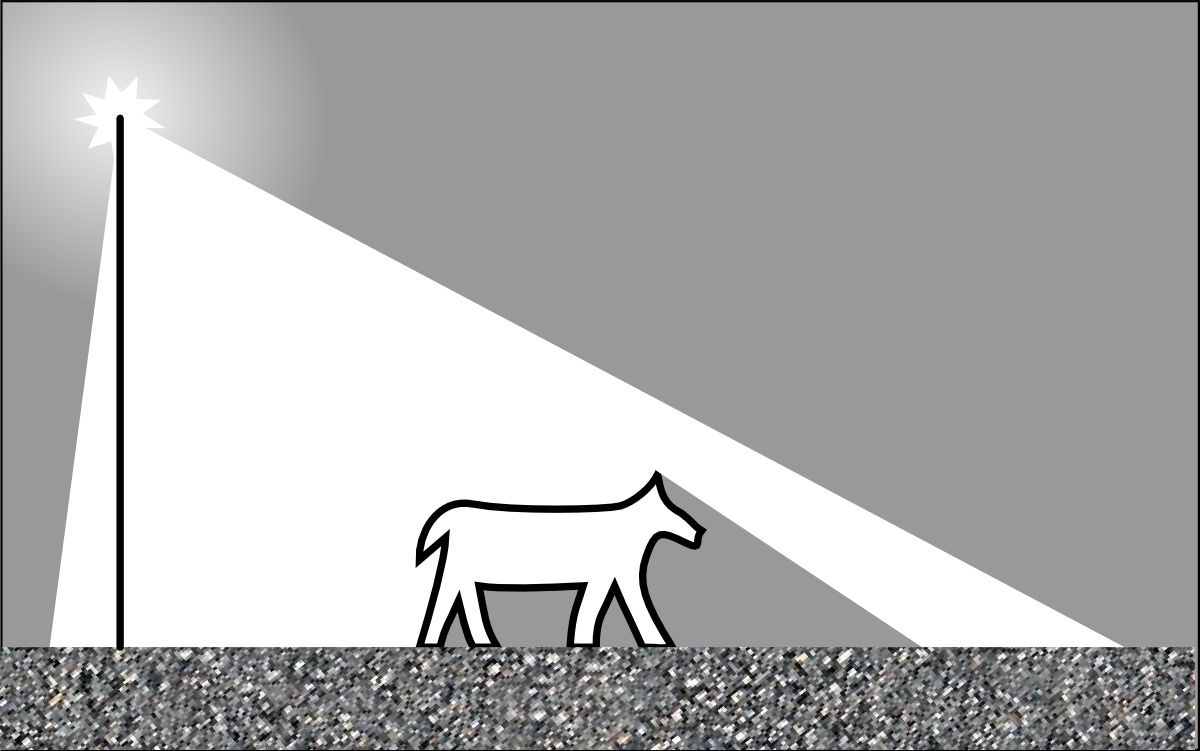
\includegraphics{04walking_dog.png}}












\problem The sides of an isosceles triangle are rotating: the lengths of 
the two (equal) sides remain fixed at 2 inch, but the angle $\theta(t)$
between them changes.




Let $A(t)$ be the area of the triangle at time $t$.  If the area increases at
a constant rate of $0.5\text{inch}^2/\text{sec}$, then how fast is the angle
increasing or decreasing when $\theta=60^\circ$?
\answer 
First, what is the area of an isosceles triangle whose sides and opening
angle you know?  This is not a formula you should memorize.  Instead try
figuring it out.  Here is the drawing:
\begin{center}
  \input ../figures/221/04problem-expandingisoscelestriangle.pdf_tex
\end{center}
The area is $\frac12 \mathsf{width}\times\mathsf{height}$, i.e.
\[
A(t)
= \mathsf{Area}
= \frac12 \times 2 \times2\sin\theta
= 2\sin\theta \; \mathsf{in}^2.
\]
This is true at all times, so we are allowed to differentiate, resulting in
\[
\frac{\dd A} {\dd t} = 2\cos \theta \frac{\dd \theta} {\dd t}.
\]
We know that $\frac{\dd A} {\dd t} = 0.5 \text{in}^2/\text{sec}$.
When $\theta=60^\circ$ we also know $\cos \theta = \frac{1} {2}$, and hence
\[
0.5 = 2\times\frac{1} {2} \times \frac{\dd \theta} {\dd t}
\text{ and thus }
\frac{\dd \theta} {\dd t} = 0.5 \mathsf{rad}/\mathsf{sec}.
\]
\endanswer




\problem A point $P$ is moving in the first quadrant of the plane.  Its motion 
is parallel to the $x$-axis; its distance to the $x$-axis is always 10 (feet).
Its velocity is 3 feet per second to the left.  We write $\theta$ for the
angle between the positive $x$-axis and the line segment from the origin to
$P$.
\answer 
The drawing:
\begin{center}
\input ../figures/221/04problem-movingpoint.pdf_tex  
\end{center}
If $x(t)$ is the $x$ coordinate of the point $P$, then
$\DS \frac{10} {x} = \tan \theta(t)$, or,
\[
10 = x\cdot \tan \theta.
\]
This is true at all times, so we may differentiate both sides
of the equation, resulting in
\[
0 = x \frac{1} {\cos^2\theta}\frac{\dd\theta} {\dd t} + \frac{\dd x} {\dd t}\tan \theta.
\]
When $\theta=\pi/3$ we have $\tan\theta = \sqrt{3}$ so $x=10/\sqrt{3}{\rm ft}$.
We are also given that $\frac{\dd x} {\dd t} = -3 {\rm ft}/{\rm sec}$
(note the minus, which
is there because the point $P$ is moving to the \emph{left}).
When $\theta=\pi/3$ we also have $\cos \theta = \frac12$.
We are led to the following equation
\[
0 = \frac{10} {\sqrt{3}} \frac{1} {(\frac12)^2} \frac{\dd \theta} {\dd t}
+ (-3) \sqrt{3},
\]
which implies
\[
 \frac{\dd \theta} {\dd t}
= 3\sqrt{3} \frac{\sqrt{3}} {10} \frac{1} {4}
= \frac{9} {40} {\rm rad}/{\rm sec}.
\]








\endanswer
\subprob  Make a drawing of the point $P$.




\subprob  Where is the point when $\theta=\pi/3$?




\subprob  Compute the rate of change of the angle $\theta$ at the moment
that $\theta=\frac\pi3$.












\problem The point $Q$ is moving on the line $y=x$ with velocity 3 m$/$sec. 
Find the rate of change of the following quantities at the moment in which
$Q$ is at the point $(1,1)$:




\subprob the distance from $Q$ to the origin,




\subprob the distance from $Q$ to the point $(2,0)$,




\subprob the angle $\angle ORQ$ where $R$ is the point $(2,0)$.








\problem A point $P$ is sliding on the parabola with equation $y=x^2$.  Its 
$x$-coordinate is increasing at a constant rate of 2 feet$/$minute.




Find the rate of change of the following quantities at the moment that
$P$ is at $(3, 9)$:




\subprob the distance from $P$ to the origin,




\subprob the area of the rectangle whose lower left corner is the origin
and whose upper right corner is $P$,




\subprob the slope of the tangent to the parabola at $P$,




\subprob the angle $\angle OPQ$ where $Q$ is the point $(0, 3)$ and $O$ is the origin $(0,0)$.




\problem \subprob The kinetic energy of a moving object with mass $m$ and velocity $v$ is $K=\frac{1}{2}mv^2$. 
If an object of mass $m=5$ grams is accelerating at a rate of $9.8$
$\textrm{m}/{\textrm{sec}^2}$, how fast is the kinetic energy increasing when
the speed is $30$ $\textrm{m}/\textrm{sec}$?




\subprob The sum of all the forces acting on the moving object is, according to
Newton, $F=ma$, where $a = \frac{dv}{dt}$.  Show that the rate at which the
kinetic energy $K$ of the object is changing is
\[
  \frac{dK}{dt} = F v.
\]




%\problem {\it Coulomb's law} states that the energy ($E$) of the interaction 
%between two ions is directly proportional to the product of the charges of two
%ions ($Q_1$ and $Q_2$) and inversely proportional to the distance ($d$) between
%their nuclei. Consider two ions of salt with charges $1+$ and $1-$. If the
%distance between the two ions is changing at a rate of $2$ pm/s, how fast is the
%energy of interaction changing when $d=165$ pm?


% The above problem has about ten errors in it: Coulomb's law is about forces and the constant of proportionality is not given, charges have units, salt is not an ion, and picometers are not defined.




\problem  Here are three versions of the same problem: 
\begin{itemize}
\item During a chemotherapy treatment, a tumor of spherical shape
  decreases in size at a rate proportional to its surface area. Show that
  the tumor's radius decreases at a constant rate.

\item Helium is released from a spherical balloon so that its volume
  decreases at a rate proportional to the balloon's surface area.  Show
  that the radius of the balloon decreases at a constant rate.

\item A spherical snowball melts at a rate proportional to its
  surface area. Show that its radius decreases at a constant rate.
\end{itemize}




\problem Suppose that we have two resistors connected in parallel with 
resistances $R_1$ and $R_2$ measured in ohms ($\Omega$).  The total
resistance, $R$, is then given by:
\[
  \frac{1}{R}=\frac{1}{R_1}+\frac{1}{R_2}.
\]
  Suppose that $R_1$ is increasing at a rate of $0.3 \Omega/\text{min}$ and $R_2$
  is decreasing at a rate of $0.5 \Omega/\text{min}$.  At what rate is $R$
changing when $R_1=80 \Omega$ and $R_2=100 \Omega$?








\problem A runner sprints around a circular track of radius $100$ meters at 
a constant speed of $7$ m/s. The runner's friend is standing at a distance
$130$ meters from the center of the track. How fast is the distance between
two friends changing when the distance between them is $130$ meters?












\problem Ship $A$ is $50$ miles north of ship $B$ and is sailing due south 
at a constant speed of $25$ mph. Ship $B$ is sailing due east at a constant speed of $20$ mph. At what rate is the
distance between the ships changing after one hour? Is the distance
increasing or decreasing?












\problem A conical water tank with vertex down has a radius of $12$ ft at 
the top and is $30$ ft high. If water flows out of the tank at a rate of
  $14$ $\text{ft}^3/\text{min}$, how fast is the depth of the water decreasing when the
water is $20$ ft deep?












\problem A train, starting at noon, travels east at $50$ mph, while another 
train leaves an hour later from the same point, traveling north at $90$ mph. How
fast are the trains moving apart at $3$ pm?












\problem The radius of a right circular cylinder is increasing at a rate of $3$ 
in/min and the height is decreasing at a rate of $5$ in/min. At what rate is the
volume changing when the radius is $10$ in and the height is $15$ in? Is the
volume increasing of decreasing?












\problem A hemispherical bowl of radius $10$ cm contains water to a depth of $h$ 
cm. Find the radius $r$ of the surface of the water as a function of $h$. The
water level drops at a rate of $0.1$ cm/hour. At what rate is the radius of
water decreasing when the depth is $5$ cm?

\problem A cylindrical swimming pool (whose center axis is vertical) is being 
filled from a fire hose at rate of $5$ cubic feet per second.  If the pool is
$40$ feet across, how fast is the water level increasing when the pool is one
third full?


\problem Consider a clock whose minute hand is $5$ cm long and whose hour hand 
is $4$ cm long.

\subprob Find the rate of change of the angle between the minute hand and hour
hand when it is $3:00$ o'clock.

\subprob Find the rate of change of the distance between the hands when it is
$3:00$ o'clock.




\problem A baseball diamond has the shape of a square, and each side is $80$ 
feet long. A player is running from second to third base, and he is $60$ feet
from reaching third. He is running at a speed of $28$ feet per second. At what
rate is the player's distance from home plate decreasing?




\problem Doppler radar measures the rate of change of the distance from an 
object to the observer. A police officer $10$ meters from a straight road points
a radar gun at a car traveling along the road, $20$ meters away, and measures a
  speed of $30 \text{m}/\text{sec}$. What is the car's actual speed?
\answer 
The situation is thus:
\begin{center}
  \input ../figures/221/04problem-dopplerpolice.pdf_tex
\end{center}
The distance from the car to the police officer is $D(t)$.
The distance along the road from the car to the nearest point to the officer
on the road is $s(t)$.  The speed of the car (which we want to know) is $s'(t)$.
The Doppler radar measures the rate at which $D(t)$ is changing.

The relation between $D(t)$ and $s(t)$ is
\[
D^2 = s^2 + (10)^2.
\]
This is true at all times so we are allowed to differentiate the relation,
which leads to
\[
2D \frac{\dd D} {\dd t} = 2s\frac{\dd s} {\dd t}
\text{ and therefore }
\frac{\dd s} {\dd t} = \frac{D} {s} \frac{\dd D} {\dd t}.
\]
Given is that at some moment $D=20$, and $\frac{\dd D} {\dd t} = -30$
(negative because the car is moving toward the officer).
``Pythagoras'' says that $s = \sqrt{D^2-(10)^2} = \sqrt{300} = 10\surd 3$.
Therefore
\[
\frac{\dd s} {\dd t} = \frac{30} {10\surd 3} \times(-30) =
-30\surd 3\; \mathrm{m}/\mathrm{sec}.
\]

Note : the phrasing of the problem is ambiguous since ``20 feet away'' could
also be taken to mean that $s=20$ when the police officer measures the car's
speed. In that case the above computation still is valid, except at the end
one must substitute $s=20$, $D = \sqrt{(20)^2 + (10)^2} = 10\surd 5$.
This leads to
$\frac{\dd s} {\dd t} = \frac{10\surd 5} {20}\times(-30) = -15\surd 5$ m$/$sec.
\endanswer

\problem A particle $A$ moves on a circular trajectory centered at the origin 
$O$, and of radius $1$, so that the angle $\alpha$ subtended by the line segment
$OA$ and the $x$-axis changes at a constant rate $k$.  Determine the rates of
change of the $x$ and $y$ coordinates of the particle.
% This problem is unclear: the angle subtended by what?


%\problem A chemical reaction between two gas molecules occurs when the molecules 
%collide with the energy greater than an activation energy $E_a$. Assume $E_a>0$
%is constant for the given gas. The fraction of bimolecular reactions in which
%this collision energy is achieved is
%\[
%  F=e^{-\frac{E_a}{k \cdot T}}
%\]
%where $T$ is the temperature and $k>0$ is Boltzmann's constant. If the
%temperature $T$ increases at a constant rate $C$, what is the rate of change of
%the fraction $F$ of collisions that result in a successful chemical reaction?
%% This problem needs to be clarified by making explicit which quantities depend on time.


\problem A crystal in the shape of a cube dissolves in acid so that the edge of 
the cube decreases by 0.3 mm/min. How fast is the volume of the cube changing
when the edge is 5 mm?








%%\problem \groupproblem  Gas is trapped in a cylinder with a piston.  The 
%%\emph{ideal gas law} from thermodynamics says that if the cylinder is
%%not heated, and if the piston moves slowly, then one has \[ pV= C T \]
%%where $p$ is the pressure in the gas, $V$ is its volume, $T$ its
%%temperature (in degrees Kelvin) and $C$ is a constant depending on the
%%amount of gas trapped in the cylinder.
%%
%%\subprob If the pressure is 10psi (pounds per square inch), if the volume
%%is $25 \text{inch}^3$, and if the piston is moving so that the gas volume is
%%expanding at a rate of $2\text{inch}^3$ per minute, then what is the rate of
%%change of the pressure?
%%
%%\subprob The ideal gas law turns out to be only approximately true.  A
%%more accurate description of gases is given by \emph{van der Waals'
%%  equation of state}, which says that
%%\[
%%\bigl(p+\frac a{V^2}\bigr)(V-b) = C
%%\]
%%where $a, b, C$ are constants depending on the temperature and the amount
%%and type of gas in the cylinder.
%%
%%Suppose that the cylinder contains fictitious gas for which one has $a=12$
%%and $b=3$.  Suppose that at some moment the volume of gas is
%%$12\text{in}^3$, the pressure is $25$psi and suppose the gas is expanding
%%at 2 inch$^3$ per minute.  Then how fast is the pressure changing?
%%
\end{multicols}
\noproblemfont


%%% Local Variables:
%%% mode: latex
%%% TeX-master: "free221"
%%% End:

% !TEX root =  free221.tex
\chapter{Graph Sketching and Max-Min Problems}
\label{ch:graph-sketching}
When we first discuss functions, one thing we want to know how to do is
determine what the graph of a function looks like.  Naively, we can produce
graphs by plugging in a number of values into a function and connecting the
points with a smooth curve. However, this is an unsatisfying method for graphing
for a variety of reasons: first, how do we know that if we find a few points on
a graph, that joining them up will actually produce the ``real'' shape of the
curve?  Second, how can we know where the ``interesting'' features of the graph
are? And third, how can we be sure that we have not missed anything?


We can provide good answers to all of these questions using calculus:
specifically, by using the first and second derivatives of a function, we can
find essentially all of the interesting features of the function's graph.




\section{Tangent and Normal lines to a graph} %{{{1
%%% !!! Discuss: move this section to the "intro derivatives" chapter, right after the definition of derivative.
The slope of the tangent to the graph of $f$ at the point $(a,
f(a))$ is
\begin{equation}
  m = f'(a)
\end{equation}
and hence the equation for the tangent line is
\begin{equation}
  \label{eq:tangent-to-graph}
  y = f(a) + f'(a) (x-a).
\end{equation}
The normal line at a point $(a,f(a))$ on the graph of a function is defined to
be the line perpendicular to the tangent line passing through that point.  The
slope of the normal line to the graph is $-1/m$ and thus one could write the
equation for the normal as
\begin{equation}
  \label{eq:normal-to-graph}
  y=f(a) - \frac{x-a}{f'(a)}.
\end{equation}
When $f'(a)=0$ the tangent is horizontal, and hence the normal is
vertical.  In this case the equation for the normal cannot be written
as in \eqref{eq:normal-to-graph}, but instead one has the simpler
equation
\[
x=a.
\]
Both cases are covered by this form of the equation for the normal
\begin{equation}
  \label{eq:normal-to-graph-all-cases}
  x=a+f'(a)(f(a)-y).
\end{equation}
Both \eqref{eq:normal-to-graph-all-cases} and \eqref{eq:normal-to-graph} are
formulas that you shouldn't try to memorize.  It is better to remember that if
the slope of the tangent is $m=f'(a)$, then the slope of the normal is $-1/m$.
\begin{figure}[h]
  \centering 
    \begin{picture} (180.000000,111.096774)(0,0)
    \put(0.0, 0.0){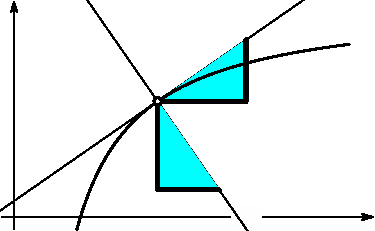
\includegraphics{05tangentAndNormal.pdf}}
        \put(181.00,   4.74){\sffamily\itshape $x$}
    \put(  4.74, 114.10){\sffamily\itshape $y$}
    \put( 60.65,  38.02){\sffamily\itshape $-1$}
    \put( 86.38,  11.80){\sffamily\itshape $m$}
    \put( 94.87,  54.25){\sffamily\itshape $1$}
    \put(120.09,  73.99){\sffamily\itshape $m$}
    \put( 84.62,  74.04){\sffamily\itshape \rotatebox{34.777831}{\footnotesize slope $=m/1=m$}}
    \put( 88.44,  48.27){\sffamily\itshape \rotatebox{-55.222169}{\footnotesize slope $=-1/m$}}
\end{picture}

  \caption{Why ``$\displaystyle \textsf{slope of normal} =
    \frac{-1}{\textsf{slope of tangent}}$.''}
  \label{fig:05tangentAndNormal}
\end{figure}




\section{The Intermediate Value Theorem} %{{{1
  % !!! Discuss: move this section to the "continuity" section.
It is said that a function is continuous if you can draw its graph without
taking your pencil off the paper.  A more precise version of this statement is
the \textit{Intermediate Value Theorem}:




\subsection{Intermediate Value Theorem} %{{{2
\itshape
If $f$ is a continuous function defined on an interval $a\leq x\leq b$, and if $y$ is
any number between $f(a)$ and $f(b)$, then there is a number $c$ with $a\leq
c\leq b$ such that $f(c) = y$.  \upshape\medskip




Here ``$y$ between $f(a)$ and $f(b)$'' means either $f(a)\leq y\leq f(b)$ or $f(b)\leq y\leq f(a)$ depending on which of $f(a)$ or $f(b)$ is larger.




The theorem should be intuitively obvious: to draw the graph you have
to start at $(a, f(a))$ and somehow move your pencil to $(b, f(b))$.
If you do this without taking your pencil off the paper, then at some
point the pencil will have to cross the horizontal line at height $y$
if $y$ is between $f(a)$ and $f(b)$.  That's what the theorem says.




However, this argument is about pencils and paper and it is not about
real numbers and solving equations.  It turns out to be difficult to
give a complete proof of the theorem.  In particular, it requires a
much better description of what a real number is than we are using in
this course.




\begin{figure}\label{fig:05intermediatevalue}
  \centering \input ../figures/221/05intermediatevalue.tex
  \caption{The Intermediate Value Theorem says that a continuous function must
    attain any given value $y$ between $f(a)$ and $f(b)$ at least once.  In this
    example there are three values of $c$ for which $f(c) = y$ holds.}
\end{figure}




\subsection{Example -- Square root of 2} %{{{2
Consider the function $f(x) = x^2$, which we know is continuous. 
Since $f(1)<2$ and $f(2) = 4>2$, the Intermediate Value Theorem with $a=1$,
$b=2$, $y=2$ tells us that there is a number $c$ between $1$ and $2$ such that
$f(c)=2$, i.e.\ for which $c^2=2$.  So the theorem tells us that ``the square
root of $2$ exists''.




\subsection{Example -- The equation $2\theta+\sin\theta=\pi$} %{{{2
    % !!! Issue: It was never proven or even mentioned that sine is continuous!
Consider the function $f(x) = 2x+\sin x$.  It is a continuous function
at all $x$, so from $f(0) = 0$ and $f(\pi) = 2\pi$ it follows that
there is a number $\theta$ between $0$ and $\pi$ such that $f(\theta)
= \pi$.  In other words, the equation
\begin{equation}\label{eq:cplussinc}
  2\theta+\sin \theta =\pi
\end{equation}
has a solution $\theta$ with $0\leq \theta\leq \pi$.  Unlike the
previous example, where we knew the solution was $\sqrt2$, there is no
simple formula for the solution to \eqref{eq:cplussinc}.

\subsection{Example -- ``Solving $1/x=0$''} %{{{2
If we attempt to apply the Intermediate Value Theorem to the function $f(x) =
1/x$ on the interval $[a,b] = [-2, 2]$, then we see that for any $y$
between $f(a) = f(-2) = -\frac12$ and $f(b) = f(2) = \frac12$ there is
a number $c$ in the interval $[-2, 2]$ such that $1/c = y$.  For
instance, we could choose $y=0$ (which lies between $-2$ and $+2$), and
conclude that there is some $c$ with $-2\leq c\leq 2$ and $1/c = 0$.




But there is no such $c$, because $1/c$ is never zero!  So we have done
something wrong: the mistake we made is that we overlooked that our function
$f(x) = 1/x$ is not defined on the \emph{entire} interval $-2\leq x\leq 2$
because it is not defined at $x=0$.  \textit{The moral: always check the
  hypotheses of a theorem before you use it!}
\marginpar{\footnotesize\sffamily%
\input ../figures/221/05intermediatevalue-fail.tex}




\section{Problems} %{{{1
\problemfont %{{{3
\begin{multicols}{2}\setlength{\parindent}{0pt}
\problem Where does the normal line to the graph of $y=x^2$ at the point (1,1) %{{{3
intersect the $x$-axis?
\answer %{{{3
At $x=3$.
\endanswer

\problem Where does the tangent line to the graph of $y=x^2$ at the point $(a, a^2)$ %{{{3
intersect the $x$-axis?
\answer %{{{3
At $x=a/2$.  
\endanswer




\problem Where does the normal line to the graph of $y=x^2$ at the point $(a, a^2)$ %{{{3
intersect the $x$-axis?
\answer %{{{3
At $x=a+2a^3$.  
\endanswer




\problem Find all points on the parabola with the equation $y = x^2 %{{{3
-1$ such that the normal line at the point goes through the origin.




\problem Where does the normal to the graph of $y=\sqrt x$ at the point $(a, %{{{3
\sqrt{a})$
intersect the $x$-axis?
\answer %{{{3
At $x=a+\frac12$.  
\endanswer








\problem Does the graph of $y=x^4-2x^2+2$ have any horizontal tangents?  If %{{{3
so, where? 

Does the graph of the same function have any vertical tangents?

Does it have vertical normals?

Does it have horizontal normals?


\problem At some point $(a, f(a))$ on the graph of $f(x) = -1+2x-x^2$, %{{{3
the tangent to this graph goes through the origin.  Which
point is it?




\problem The line from the origin to the point $(a, f(a))$ on the graph of $f(x) %{{{3
= 1/x^2$ is perpendicular to the tangent line to that graph.  What is $a$?




\problem The line from the origin to the point $(a, f(a))$ on the graph of $f(x) %{{{3
= 4/x$ is perpendicular to the tangent line to the graph.  What is $a$?




\problem Find equations for the tangent and normal lines %{{{3




\textbf{to the curve \ldots} \hfill \textbf{at the point\ldots}\\
\subprob $y=4x/(1+x^2) $ \hfill $(1, 2)$\\
\subprob $y=8/(4+x^2) $ \hfill $(2, 1)$\\
\subprob $y^2=2x+x^2$ \hfill $(2, 2)$\\
\subprob $xy=3$ \hfill $(1, 3)$\\












\problem \groupproblem The function $$f(x) = \frac{x^2+|x|}{x}$$ satisfies $f(-1) = %{{{3
-2$ and $f(+1) = +2$, so, by the Intermediate Value Theorem,
there should be some value $c$ between $-1$ and $+1$ such that
$f(c) = 0$.  \emph{True or False?}
\answer %{{{3
False.  If you try to solve $f(x) = 0$, then you get the equation
$\frac{x^2+|x|}{x}=0$.  If $x\ne0$ then this is the same as
$x^2+|x|=0$, which has no solutions (both terms are positive when
$x\ne0$).  If $x=0$ then $f(x)$ isn't even defined.
So there is no solution to $f(x) = 0$.




This doesn't contradict the IVT, because the function isn't
continuous, in fact it isn't even defined at $x=0$, so the IVT
doesn't have to apply.  
\endanswer


\problem Find the equation for the tangents to the graph of the Backward Sine %{{{3
\[
  f(x)=\sin\left(\dfrac{\pi}{x}\right)
\]
at the points $x=1$, $x=\frac12$ and at $D$  (see Figure \ref{fig:03sinePiOverx}
in \S\ref{sec:03backward-sine}.)




\problem Find the equation for the tangent to the graph of the Backward Cosine %{{{3
in a Bow Tie $g(x)=x\cos\left(\dfrac{\pi}{x}\right)$ at the point $C$  (see Figure
\ref{fig:03backwardCosSandwich} in \S\ref{sec:03xcos1overx})
\end{multicols}




\noproblemfont

\section{Finding sign changes of a function}\label{sec:sign-changes} %{{{1
The Intermediate Value Theorem implies the following very useful fact.

\subsection{Theorem} %{{{2
\label{thm:nosignchangebetweenzeros}\itshape
If $f$ is a continuous function on an interval $a\leq x\leq b$, and if
$f(x)\neq0$ for all $x$ in this interval, then $f(x)$ does not change
its sign in the interval $a\leq x\leq b$: either $f(x)$ is
positive for all $a\leq x\leq b$, or it is negative for all $a\leq x\leq b$.
\upshape




\begin{proof}
  The theorem says that there cannot be two numbers $a \leq x_1<x_2 \leq b$ such
  that $f(x_1)$ and $f(x_2)$ have opposite signs.  If there were two
  such numbers then the Intermediate Value Theorem would imply that
  somewhere between $x_1$ and $x_2$ there would be a $c$ with $f(c)=0$.
  But we are assuming that $f(c)\neq0$ whenever $a \leq c \leq b$. This is a contradiction, so no such $x_1$ and $x_2$ can exist.
\end{proof}




\subsection{Example} %{{{2
Consider
\[
f(x) = (x-3)(x-1)^2(2x+1)^3.
\]
The zeros of $f$ (the solutions of $f(x)=0$) are $ -\frac12, 1, 3 $.
These numbers split the real line into four intervals
\[
(-\infty, -\tfrac12), \quad (-\tfrac12, 1), \quad (1, 3),\quad (3, \infty).
\]
Theorem \ref{thm:nosignchangebetweenzeros} tells us that $f(x)$ cannot change
its sign in any of these intervals.  For instance, $f(x)$ has the same sign for
all $x$ in the first interval $(\infty, -\frac12)$.  Now we choose a number we
like from this interval, say $-1$, and determine that the sign of $f(-1)$:
$f(-1) =(-4)(-2)^2(-1)^3$ is positive.  Therefore $f(x) >0$ for all $x$ in the
interval $(-\infty, -\tfrac12)$.  In the same way we find
\begin{eqnarray*}
  f(-1) = (-4)(-2)^2(-1)^3>0 &\implies & f(x) >0 \text{ for } x<-\tfrac12\\
  f( 0) = (-3)(-1)^2( 1)^3<0 &\implies & f(x) <0 \text{ for } -\tfrac12<x<1\\
  f( 2) = (-1)( 1)^2( 5)^3<0 &\implies & f(x) <0 \text{ for } 1<x<3\\
  f( 4) = ( 1)( 3)^2( 9)^3>0 &\implies & f(x) >0 \text{ for } x>3.
\end{eqnarray*}
If we know all the zeroes of a continuous function, then this method allows us
to decide where the function is positive or negative.  However, when the given
function is factored into easy functions, as in this example, there is a
different way of finding the signs of $f$.  For each of the factors $x-3$,
$(x-1)^2$ and $(2x+1)^3$ it is easy to determine the sign, for any given $x$.
These signs can only change at a zero of the factor.  Thus we have
\begin{itemize}
\item $x-3$ is positive for $x>3$ and negative for $x<3$;
\item $(x-1)^2$ is always positive (except at $x=1$);
\item $(2x+1)^3$ is positive for $x>-\frac12$ and negative for $x<-\frac12$.
\end{itemize}
Multiplying these signs we get the same conclusions as above. We can summarize
this computation in the following diagram:
\begin{figure}[h]
  \centering\sffamily
  \input{../figures/221/05signs-of-f.pdf_tex}
\end{figure}
















\section{Increasing and decreasing functions} %{{{1
Here are four very similar definitions -- look closely to see how they differ.
\begin{itemize}
\item A function is called \emph{increasing} on an interval if $a<b$ implies
  $f(a)<f(b)$ for all numbers $a$ and $b$ in the interval.

\item A function is called \emph{decreasing} on an interval if $a<b$ implies $f(a)>f(b)$ for
  all numbers $a$ and $b$ in the interval.

\item The function $f $ is called \emph{non-decreasing} on an interval if $a<b$ implies
  $f(a)\leq f(b)$ for all numbers $a$ and $b$ in the interval.




\item The function $f $ is called \emph{non-increasing} on an interval if $a<b$ implies
  $f(a)\geq f(b)$ for all numbers $a$ and $b$ in the interval.
\end{itemize}
We can summarize these definitions as follows:
\begin{align*}
 on an interval, \textbf{$f$ is \ldots}\quad\quad&
                           \textbf{if for all $a$ and $b$ in the interval\ldots}\\
  \text{Increasing:}\quad & a<b \implies f(a)<f(b) \\
  \text{Decreasing:}\quad & a<b \implies f(a)>f(b) \\
  \text{Non-increasing:}\quad & a<b \implies f(a)\geq f(b) \\
  \text{Non-decreasing:}\quad & a<b \implies f(a)\leq f(b)
\end{align*}




The definitions of increasing, decreasing, non-increasing, and non-decreasing do
not seem like they are easy to check for a particular function.  But, in fact,
there is an easy test for whether a function is increasing or decreasing: look
at the sign of the derivative of $f$.  More precisely:




\subsection{Theorem}\label{thm:increasing-implies-deriv-pos} %{{{2
\itshape If a differentiable function is non-decreasing on an interval then
$f'(x)\geq 0$ for all $x$ in that interval.

If a differentiable function is non-increasing on an interval then $f'(x)\leq 0$
for all $x$ in that interval.  \upshape

The idea of the proof is the following: if $f$ is non-decreasing, then for any given $x$ and any positive
$\Delta x$, we have $f(x+ \Delta x)\geq f(x)$, so
\[
\frac{f(x+ \Delta x)-f(x)}{\Delta x} \geq 0.
\]
Now if we let $\Delta x\searrow 0$, we see
\[
f'(x) = \lim_{\Delta x\searrow0}\frac{f(x+ \Delta x)-f(x)}{\Delta x} \geq 0.
\]


What about the converse?  In other words, if we know the sign of $f'$ then what can we
say about $f$?  For this we have the following
\subsection{Theorem} %{{{2
\label{thm:deriv-pos-implies-increasing}\itshape
Suppose $f$ is a differentiable function on an interval $(a,b)$.

If $f'(x)>0$ for all $a<x<b$, then $f$ is increasing on the interval.

If $f'(x)<0$ for all $a<x<b$, then $f$ is decreasing on the interval.\upshape
\medskip




The proof is based on the Mean Value Theorem, which also finds use in
many other situations:
\subsection{The Mean Value Theorem} %{{{2
  % !!! Discuss: What is the point of proving the first derivative test via the MVT, without even explaining the MVT or its proof??
\itshape
If $f$ is a differentiable function on the interval $a\leq x\leq b$,
then there is some number $c$ with $a<c<b$ such that
\[
f'(c) = \frac{f(b)-f(a)}{b-a}.
\]
\upshape




\begin{figure}[t]\flushleft\sffamily



  \color{darkbluegreen}
  \parbox[b]{0.45\textwidth}{\textbf{The Mean Value Theorem }says that
    if you pick any two points $A$ and $B$ on the graph of a differentiable function,
    then there always is a point on the graph between $A$ and $B$
    where the tangent line to the graph is parallel to the line segment
    $AB$.  Depending on the shape of the graph and the location of the
    points $A$, $B$, there may even be more than one such point (there are two
    in this figure).  The MVT is used in the proofs of many facts
    about functions; for instance,
    Theorem~\ref{thm:deriv-pos-implies-increasing}.  Here is a picture
  proof of the Mean Value Theorem:}
  \hfill
  \parbox[b]{0.4\textwidth}{\input ../figures/221/05mvt2.tex }




  \def\mvtprooftextone{%
    \parbox[t]{80pt}{\sffamily\itshape\footnotesize\color{darkbluegreen}%
      To find a point on this curve where the tangent is parallel to
      the chord $AB$, you draw two lines \ldots}}




  \def\mvtprooftexttwo{%
    \parbox[b]{96pt}{\sffamily\itshape\footnotesize\color{darkbluegreen}%
      \ldots parallel to the chord, one far above the graph
      and one far below the graph.  Then, always keeping these lines
      parallel to the chord,  you slide them towards the graph \ldots }}




  \def\mvtprooftextthree{%
    \parbox[b]{96pt}{\sffamily\itshape\footnotesize\color{darkbluegreen}%
      \ldots until they touch the
      graph.  At the points where the lines touch the graph, the
      tangent line to the graph is parallel to the chord $AB$. }}
  
  \def\mvtproofthechord{{\sffamily\itshape\footnotesize\color{darkbluegreen} The
  chord $AB$}}

  \input{../figures/221/05mvt-proof.pdf_tex}




  \caption{The Mean Value Theorem}
  \label{fig:05MeanValueTheorem}
  \rule{\textwidth}{2pt}
\end{figure}








\begin{proof}[Proof of theorem \ref{thm:deriv-pos-implies-increasing}]
  We show that $f'(x)>0$ for all $x$ implies that $f$ is increasing.
  (The proof of the other statement is very similar.)
  Let $x_1<x_2$ be two numbers between $a$ and $b$.  Then the Mean Value Theorem
  implies that there is some $c$ between $x_1$ and $x_2$ such that
  \[
  f'(c) = \frac{f(x_2)-f(x_1)}{x_2-x_1},
  \]
  or
  \[
  f(x_2)-f(x_1) = f'(c) (x_2-x_1).
  \]
  Since we know that $f'(c)>0$ and $x_2-x_1>0$ it follows that
  $f(x_2)-f(x_1)>0$, or $f(x_2)>f(x_1)$.
\end{proof}




\section{Examples} %{{{1
Armed with these theorems we can now split the graph of any function into
increasing and decreasing parts simply by computing the derivative $f'(x)$ and
finding out where $f'(x)>0$ and where $f'(x)<0$, and to do this we need only apply the method
  from \ref{sec:sign-changes} to $f'$ rather than $f$.




\subsection{Example: the parabola $y=x^2$} %{{{2
The familiar graph of $f(x)=x^2$ consists of two parts, one decreasing and one
increasing, separated by $x=0$.  You can see this from the derivative which is
\[
f'(x) = 2x
\begin{cases}
  >0 & \text{for $x>0$} \\
  <0 & \text{for $x<0$.}
\end{cases}
\]
Therefore the function $f(x) = x^2$ is \emph{decreasing for $x<0$} and
\emph{increasing for $x>0$.}


% !!! TO-DO: Caption these figures
\begin{figure}[h]
  \centering
  \parbox{170pt}{\input ../figures/221/05parabola.tex}
  \quad
  \parbox{170pt}{\input ../figures/221/05hyperbola.tex}
\end{figure}




\subsection{Example: the hyperbola $ y=1/x $} %{{{2
The derivative of the function $f(x)= 1/x = x^{-1}$ is
\[
f'(x) = -\frac{1}{x^2}
\]
which is always negative.  One might therefore think that this function is
decreasing, or at least non-increasing: if $a<b$ then $1/a \geq 1/b$.  But this
isn't true if we take $a=-1$ and $b=1$:
\[
a=-1<1=b, \text{ but } \frac{1}{a} = -1 < 1 = \frac{1}{b}\text{ !!}
\]
The problem is that we attempted to use theorem
\ref{thm:deriv-pos-implies-increasing}, but this function only applies to
functions \emph{that are defined on an interval}.  The function in this example,
$f(x)=1/x$, is not defined on the interval $-1<x<1$, because it isn't defined at
$x=0$.  That's why we can't conclude that $f(x) = 1/x$ is increasing from $x=-1$
to $x=+1$.




On the other hand, the function is defined and differentiable on the interval
$0<x<\infty$, so theorem \ref{thm:deriv-pos-implies-increasing} tells us that
$f(x) = 1/x$ is decreasing for $x>0$.  This means, that as long as $x$ is
positive, increasing $x$ will decrease $1/x$.




\begin{figure}[t]
  \centering 
    \begin{picture} (270.000000,270.000000)(0,0)
    \put(0.0, 0.0){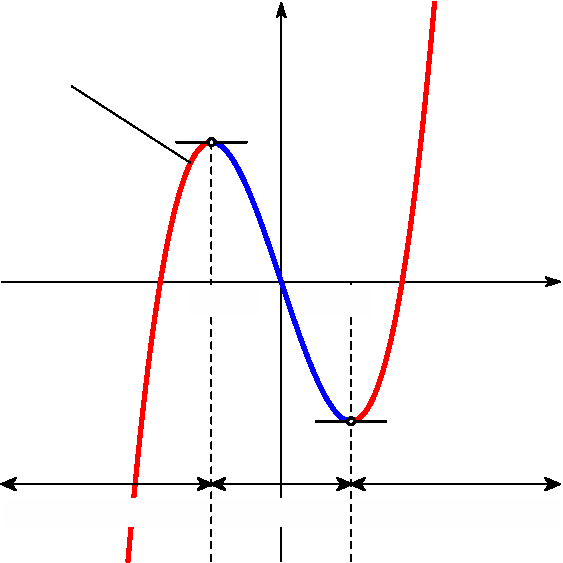
\includegraphics{05upAndDown.pdf}}
        \put( 51.25,  24.50){\sffamily\itshape \makebox[0pt][c]{$f'(x)>0$}}
    \put(218.75,  24.50){\sffamily\itshape \makebox[0pt][c]{$f'(x)>0$}}
    \put(135.00,  24.50){\sffamily\itshape \makebox[0pt][c]{$f'(x)<0$}}
    \put(156.50, 123.00){\sffamily\itshape $x=+1$}
    \put( 89.50, 123.00){\sffamily\itshape $x=-1$}
    \put( 34.50, 235.50){\sffamily\itshape \makebox[0pt][c]{\framebox{$y=x^3-3x$}}}
\end{picture}





  \bigskip




  \caption{The graph of $f(x) = x^3-3x$.}
  \label{fig:05upAndDown}
\end{figure}




\subsection{Graph of a cubic function} %{{{2
\label{sec:cubicgraph}
Consider the function
\[
y = f(x) = x^3-3x.
\]
Its derivative is $f'(x) = 3x^2-3$.  We try to find out where $f'$ is positive,
and where it is negative by factoring $f'(x)$:
\[
f'(x) = 3(x^2-1)
=3(x-1)(x+1)
\]
from which we see that
\begin{align*}
  f'(x) > 0 &\text{ for }x<-1 \\
  f'(x) < 0 &\text{ for }-1 < x < 1 \\
  f'(x) > 0 &\text{ for } x>1
\end{align*}
Therefore the function $f$ is
\begin{center}
  increasing on $(-\infty, -1)$, \quad decreasing on
  $(-1, 1)$, \quad increasing on
  $(1, \infty)$.
\end{center}
At the two points $x=\pm1$ one has $f'(x)=0$ so there the tangent
is horizontal.  This leads to Figure~\ref{fig:05upAndDown}.




\subsection{A function whose tangent turns up and down infinitely often near the origin} %{{{2
We end this section with a weird example.  Somewhere in the mathematician's zoo
of curious functions the following will be on exhibit.  Consider the function
\[
f(x) = \frac x2+x^2\sin\frac\pi x.
\]
(See Figure~\ref{fig:05zigzagBetweenParabolas}.)  For $x=0$ this
formula is undefined so that we still have to define $f(0)$.  We
choose $f(0)=0$.  This makes the function continuous at $x=0$. In
fact, this function is differentiable at $ x=0 $, with derivative
given by
\[
f'(0) = \lim_{x\to 0}\frac{f(x)-f(0)}{x-0} =\lim_{x\to0} \frac12+x\sin\frac\pi
x=\frac12.
\]
(To find the limit, apply the sandwich theorem to $-|x| \leq
x\sin\tfrac\pi x \leq |x|$, as in \S~\ref{sec:backward-cosine-sandwich}.)
\begin{figure}[t]
  \centering 
    \begin{picture} (300.000000,300.000000)(0,0)
    \put(0.0, 0.0){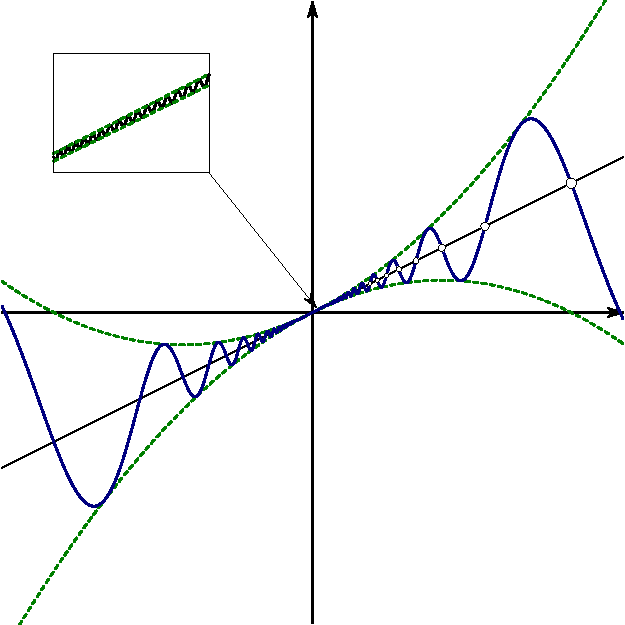
\includegraphics{05zigzagBetweenParabolas2.pdf}}
        \put( 25.83, 207.05){\sffamily\itshape \makebox[0pt][c]{\texttt{\upshape\footnotesize 0.005}}}
    \put(100.33, 207.05){\sffamily\itshape \makebox[0pt][c]{\texttt{\upshape\footnotesize 0.006}}}
    \put( 25.83, 286.17){\sffamily\itshape \makebox[0pt][l]{\parbox{76pt}{\footnotesize\sffamily 
magnification of the graphs near the origin}}}
    \put(278.17, 274.17){\sffamily\itshape $y=\frac 12x+x^2$}
    \put(303.00, 132.10){\sffamily\itshape $y=\frac 12x-x^2$}
    \put(302.00, 224.50){\sffamily\itshape $y=\frac 12x$}
    \put(288.58, 179.68){\sffamily\itshape $y=\frac 12x+x^2\sin\frac\pi x$}
\end{picture}

  \caption{The function $y = \frac12 x+ x^{2}\sin\frac\pi x$ is
    differentiable, and at $x=0$ its derivative is positive (namely,
    $1/2$).  You would think that this means that the function
    therefore has to be increasing near $x=0$, but this example shows
    that the function doesn't have to be increasing near $x=0$.  You
    can see that by zooming in on the graph near the origin.  As you
    follow the graph of $y = \frac12 x+ x^{2}\sin\frac\pi x$ to the
    origin it alternates between increasing and decreasing infinitely
    often.  \label{fig:05zigzagBetweenParabolas}}
\end{figure}




\noindent
The slope of the tangent to the graph at the origin is positive
($\frac12$), and you would \textit{think} that the function should be
``increasing near $x=0$'' But this turns out not to be true!

To see why not, compute the derivative of this function for
$x\neq0$:
\[
f'(x) = \frac12-\pi\cos\frac\pi x+2x\sin\frac\pi x.
\]
We could try to find where $f'(x)$ is positive, and where it's negative, just as
we did for $y=x^3-3x$ in \S~\ref{sec:cubicgraph}, but for this function solving
$f'(x)=0$ turns out to be pretty much impossible.  Fortunately, even though we
can't solve $f'(x) = 0$, we can still find out something about the derivative by
looking at the intersection points of the graph with the line $y=x/2$ and
checking the sign of $f'(x)$ at those points.  We will find that $f'(x)$
flip-flops infinitely often between positive and negative as $x \searrow 0$.  




There are infinitely many intersection points of $y=f(x)$ with $y=x/2$ and the coordinates are
\[
x_k= \frac1k,\quad y_k= f(x_k).
\]
For larger and larger $k$ the points $(x_k, y_k)$ tend to the origin (the $x$
coordinate is $\frac1k$ which goes to 0 as $k\to\infty$).  The slope of the
tangent at $x=x_k$ is given by
\begin{align*}
  f'(x_k) &= \frac12-\pi\cos\frac\pi{1/k} +2\frac1k\sin\frac\pi{1/k}\\
  &= \frac12-\pi \underbrace{\cos k\pi}_{=(-1)^k} +\frac2k
  \underbrace{\sin k\pi}_{=0}\\
  &=\begin{cases}
    \frac12-\pi<0 & \text{for $k$ even}\\[4pt]
    \frac12+\pi>0 & \text{for $k$ odd}
  \end{cases}
\end{align*}
Therefore, along the sequence of points $(x_k, y_k)$ the slope of the tangent
jumps back and forth between $\frac12-\pi$ and $\frac12+\pi$, i.e. between a
positive and a negative number.
In particular, the slope of the tangent at the odd intersection points is
negative, and so you would expect the function to be decreasing there.  
We see that \textit{even though the derivative at $x=0$ of this
particular function is positive, there are points on the graph arbitrarily close
to the origin where the tangent has negative slope.}








\section{Maxima and Minima} %{{{1
A function has a \emph{global maximum} at some $a$ in its domain if $f(x)\leq
f(a)$ for all other $x$ in the domain of $f$.  Global maxima are sometimes also
called ``absolute maxima''.
  
A function has a \emph{global minimum} at some $a$ in its domain if $f(x)\geq
f(a)$ for all other $x$ in the domain of $f$.  Global minima are sometimes also
called ``absolute minima''.




A function has a \emph{local maximum} at some $a$ in its domain if
there is a small $\delta>0$ such that $f(x)\leq f(a)$ for all $x$ with
$a-\delta<x<a+\delta$ that lie in the domain of $f$.
  
A function has a \emph{local minimum} at some $a$ in its domain if
there is a small $\delta>0$ such that $f(x)\leq f(a)$ for all $x$ with
$a-\delta<x<a+\delta$ that lie in the domain of $f$.




Every global maximum is a local maximum, but a local maximum doesn't have to be
a global maximum.
\begin{figure}[h]
  \centering{ 
    \begin{picture} (240.000000,150.750000)(0,0)
    \put(0.0, 0.0){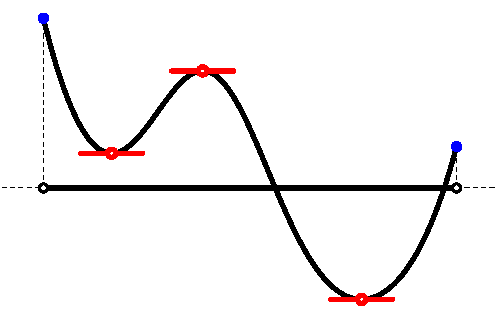
\includegraphics{05minsAndMaxes.pdf}}
        \put( 18.83,  48.50){\sffamily\itshape $a$}
    \put(217.17,  48.50){\sffamily\itshape $b$}
    \put(  8.83, 147.96){\sffamily\itshape {\footnotesize\sffamily\itshape abs max}}
    \put(207.17,  86.35){\sffamily\itshape {\footnotesize\sffamily\itshape loc max}}
    \put( 85.27, 122.67){\sffamily\itshape {\footnotesize\sffamily\itshape loc max}}
    \put( 41.60,  69.18){\sffamily\itshape {\footnotesize\sffamily\itshape loc min}}
    \put(161.59,  -1.01){\sffamily\itshape {\footnotesize\sffamily\itshape abs min}}
\end{picture}
}
  \caption{A function defined on an interval $[a, b]$ with one interior absolute
    minimum, another interior local minimum, an interior local maximum, and two
    local maxima on the boundary, one of which is in fact an absolute maximum.}
  \label{fig:05maxAndMins}
\end{figure}

\subsection{How to find local maxima and minima} %{{{2
\label{sec:where-find-maxes}
Any $x$ value for which $f'(x) = 0$ is called a \emph{stationary point} for the
function $f$.




\begin{theorem}\label{thm:zero-deriv-at-extrema}
  Suppose $f$ is a differentiable function on an interval $[a,b]$.




  Every local maximum or minimum of $f$ is either one of the end points of the
  interval $[a,b]$, or else it is a stationary point for the function $f$.
\end{theorem}




\begin{proof}
  Suppose that $f $ has a local maximum at $x$ and suppose that $x$ is not $a$
  or $b$.  By assumption the left and right hand limits
  \[
  f'(x) = \lim_{\Delta x\nearrow 0}\frac{f(x+\Delta x)-f(x)}{\Delta x} \text{
    and } f'(x) = \lim_{\Delta x\searrow 0}\frac{f(x+\Delta x)-f(x)}{\Delta x}
  \]
  both exist and they are equal.




  Since $f$ has a local maximum at $x$ we have $f(x+\Delta x)-f(x)\leq 0$ if
  $-\delta<\Delta x<\delta$.  In the first limit we also have $\Delta x<0$, so
  that
  \[
  \lim_{\Delta x\nearrow 0}\frac{f(x+\Delta x)-f(x)}{\Delta x} \geq 0.
  \]
  Hence $f'(x) \geq 0$.
% !!! Minor issue: This needs a reference to the limit theorem about inequalities.


  In the second limit we have $\Delta x>0$, so
  \[
  \lim_{\Delta x\searrow 0}\frac{f(x+\Delta x)-f(x)}{\Delta x} \leq 0,
  \]
  which implies $f'(x)\leq 0$.




  Thus we have shown that $f'(x)\leq0$ and $f'(x)\geq 0$ at the same time.  This
  can only be true if $f'(x) = 0$.
\end{proof}




\subsection{How to tell if a stationary point is a maximum, a minimum, or neither} %{{{2
\label{sec:isitamaxormin}
If $f'(c)=0$ then $c$ is a stationary point (by definition), and it might be
local maximum or a local minimum.  You can tell what kind of stationary point
$c$ is by looking at the sign of $f'(x)$ for $x$ near $c$.




\begin{theorem}\label{thm:max-min-test}
  Suppose $y=f(x)$ is function that is defined in an interval
  $(c-\delta, c+\delta)$, where $\delta>0$ is some (small) number.
  \begin{trivlist}
  \item[$\bullet$] If $f'(x)>0$ for $x<c$ and $f'(x)<0$ for $x>c$ then $f$ has a
    local maximum at $x=c$.
  \item[$\bullet$] If $f'(x)<0$ for $x<c$ and $f'(x)>0$ for $x>c$ then $f$ has a
    local minimum at $x=c$.
  \end{trivlist}
\end{theorem}%
\marginpar{\sffamily\itshape\footnotesize%
  \input ../figures/221/05updown-means-max.pdf_tex \\
  \input ../figures/221/05downup-means-min.pdf_tex }
\smallskip




The reason is simple: if $f$ increases to the left of $c$ and decreases to the
right of $c$ then it has a maximum at $c$.  More precisely:




\begin{enumerate}




\item if $f'(x)>0$ for $x$ between $c-\delta$ and $c$, then $f$ is
  increasing for $c-\delta<x<c$ and therefore $f(x)<f(c)$ for $x$
  between $c-\delta$ and $c$.








\item If in addition $f'(x)<0$ for $x>c$ then $f$ is decreasing for
  $x$ between $c$ and $c+\delta$, so that $f(x)<f(c)$ for those $x$.

\item Combining (1) \& (2) gives $f(x)\leq f(c)$ for
  $c-\delta<x<c+\delta$.
\end{enumerate}
The statement about when $f$ has a local minimum follows from an analogous argument.


\subsection{Example -- local maxima and minima of $f(x) = x^3-3x$} %{{{2
\label{sec:locmaxminofcubic}%
In \S\ref{sec:cubicgraph} we found that the function $f(x) =
x^3-3x$ is increasing when $-\infty<x<-1$, and also when $1<x<\infty$,
while it is decreasing when $-1<x<1$.  It follows that the function
has a local maximum at $x=-1$, and a local minimum at $x=1$.

Neither the local maximum nor the local minimum are global since
\[
\lim_{x\to-\infty} f(x) = +\infty\text{ and } \lim_{x\to\infty} f(x) = -\infty.
\]


\subsection{A stationary point that is neither a maximum nor a minimum} %{{{2
If you look for stationary points of the function $f(x) = x^3$ you will find that
there's only one, namely $x=0$.  The derivative $f'(x)=3x^2$ does not change
sign at $x=0$, so the test in Theorem~\ref{thm:max-min-test} does not say
anything.




And in fact, $x=0$ is neither a local maximum nor a local minimum because
$f(x)<f(0)$ for $x<0$ and $f(x)>0$ for $x>0$.
\marginpar{%
  
    \begin{picture} (90.000000,90.000000)(0,0)
    \put(0.0, 0.0){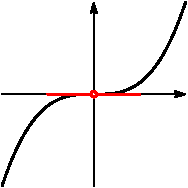
\includegraphics{05neitherMaxNorMin.pdf}}
        \put( 53.80,  80.20){\sffamily\itshape $y=x^3$}
\end{picture}
}

\section{Must a function always have a maximum?} %{{{1
\label{sec:max-exists}
Theorem~\ref{thm:zero-deriv-at-extrema} is very useful since it tells
you how to find (local) maxima and minima.  The following theorem is
also useful, but in a different way.  It doesn't say how to find
maxima or minima, but it tells you that they do exist, and hence that
you are not wasting your time trying to find them.




\begin{theorem}\label{thm:max-min-exist}
  Let $f$ be continuous function defined on the \emph{closed} interval
  $a\leq x\leq b$.  Then $f$ attains its absolute maximum somewhere in this
  interval, and it also attains its absolute minimum somewhere in the interval.
  In other words, there exist real numbers $c$ and $d$ between $a$ and $b$ such that
  \[
  f(c)\leq f(x) \leq f(d)
  \]
  whenever $a\leq x\leq b$.
\end{theorem}\smallskip




This is another one of those theorems whose proof requires a more
careful definition of the real numbers than we have given in Chapter
1.  In this course we will take the theorem for granted.




\section{Examples -- functions with and without maxima or minima} %{{{1
In the following three example we explore what can happen if some of the
hypotheses in Theorem~\ref{thm:max-min-exist} are not met.




\begin{figure}[h]\centering
  \begin{minipage} {110pt}
    
    \begin{picture} (100.000000,93.000000)(0,0)
    \put(0.0, 0.0){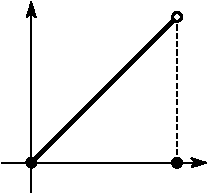
\includegraphics{05xnomax.pdf}}
        \put( 85.00,   3.00){\sffamily\itshape $1$}
    \put( 83.00,  19.00){\sffamily\itshape \makebox[0pt][r]{$f(1)=0$}}
    \put( 13.00,  17.00){\sffamily\itshape \makebox[0pt][r]{min}}
    \put( 90.00,  85.00){\sffamily\itshape \makebox[0pt][l]{max?}}
\end{picture}

  \end{minipage}
  \hfill
  \begin{minipage}{240pt}
    
    \begin{picture} (235.000000,64.730769)(0,0)
    \put(0.0, 0.0){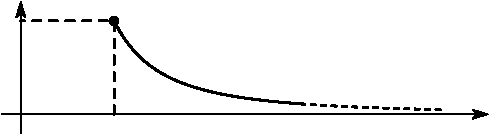
\includegraphics{05xinv_nomin.pdf}}
        \put( 52.77,  -2.04){\sffamily\itshape 1}
    \put( -2.04,  50.77){\sffamily\itshape 1}
    \put( 99.58,  25.16){\sffamily\itshape \makebox[0pt][l]{$y=1/x^2$}}
    \put( 57.77,  58.77){\sffamily\itshape \makebox[0pt][c]{max}}
    \put(211.60,  14.44){\sffamily\itshape \makebox[0pt][c]{min?}}
\end{picture}

  \end{minipage}
  \caption{The function on the left has no maximum, and the one on the right has
    no minimum.}\label{fig:05nomaxnomin}
\end{figure}
\subsection{Question: } %{{{2
\itshape Does the function
\[
f(x) =
\begin{cases}
  x & \text{for }0\leq x<1 \\ 0 &\text{ for }x=1.
\end{cases}
\]
have a maximum on the interval $0\leq x\leq 1$?\upshape




\subsection*{Answer: } %{{{2
No.  What would the maximal value be?  Since
\[
\lim_{x\nearrow1}f(x) = \lim_{x\nearrow1}x = 1,
\]
the maximal value cannot be less than 1.  On the other hand the function is
never larger than $1$.  So if there were a number $a$ in the interval $[0,1]$
such that $f(a)$ was the maximal value of $f$, then we would have to have $f(a) = 1$.
But such an $a$ does not exist!  Conclusion: this function does \emph{not}
attain its maximum on the interval $[0,1]$.




What about Theorem~\ref{thm:max-min-exist}?  That theorem only applies to
continuous functions, and the function $f$ in this example is not continuous at
$x=1$.  It's not continuous because at $x=1$ we have
\[
f(1) = 0, \text{ which is not the same as } \lim_{x\nearrow1} f(x)=1.
\]
So all it takes for Theorem~\ref{thm:max-min-exist} to fail is that
the function $f$ be discontinuous at \textit{just one point}.




\subsection{Question: } %{{{2
\itshape Does the function
\[
f(x) = \frac1{x^2}, \quad 1\leq x<\infty
\]
have a maximum or minimum?\upshape




\subsection*{Answer: } %{{{2
The function has a maximum at $x=1$, but it has no
minimum.




Concerning the maximum: if $x\geq 1$ then $f(x) = 1/{x^2}\leq1$, while
$f(1) = 1$.  Hence $f(x)\leq f(1)$ for all $x$ in the interval $[1,
\infty)$. By definition, this means that $f$ attains its maximum at
$x=1$.








If we look for a minimal value of $f$ then we note that $f(x)\geq0$ for all $x$
in the interval $[1,\infty)$, and also that
\[
\lim_{x\to\infty} f(x) = 0,
\]
so that \emph{if} $f$ attains a minimum at some $a$ with $1\leq a<\infty$, then
the minimal value $f(a)$ must be zero.  However, the equation $f(a) = 0$ has no
solution: $f$ does not attain its minimum.








\subsubsection*{Why did Theorem \ref{thm:max-min-exist} fail this time? }
In this example the function $f$ is continuous on the whole interval
$[1,\infty)$, but this interval is not a closed interval of the
form $[a,b]$.




\section{General method for sketching the graph of a function} %{{{1
  % !!! Issue: Graph-sketching requires concavity information! This section
  % should be moved after the concavity section!
Given a differentiable function $f$ defined on an interval $a\leq x\leq b$,
we can find the increasing and decreasing parts of the graph along with the local maxima and minima by following this procedure:




\begin{enumerate}
\item find all solutions of $f'(x)=0$ in the interval $[a,b]$: these are called
  the \textit{critical} or \textit{stationary} points for $f$.
\item find the sign of $f'(x)$ at all other points
\item each stationary point at which $f'(x)$ actually changes sign is a local
  maximum or local minimum.  Compute the function value $f(x)$ at each
  stationary point.
\item compute the function values at the endpoints of the interval, i.e.\
  compute $f(a)$ and $f(b)$.
\item the absolute maximum is attained at the stationary point or the boundary
  point with the highest function value; the absolute minimum occurs at the
  boundary or stationary point with the smallest function value.
\end{enumerate}
If the interval is unbounded, then instead of computing the values $f(a)$ or
$f(b)$, but instead you should compute $\lim_{x\to\pm\infty}f(x)$.




\subsection{Example -- the graph of a rational function} %{{{2
  % !!! TO-DO: change this function so that the roots of the derivative aren't
  % horrible Remark: If the function is changed to x(3-4x)/(1+x^2) it looks
  % basically identical but the roots of the derivative are much nicer!
Let's sketch the graph of the function
\[
f(x) = \frac{3x(1-x)}{1+x^2}.
\]
By looking at the signs of numerator and denominator we see that
\begin{center}
  $f(x)>0$ for $0<x<1$\\[2pt]
  $f(x)<0$ for $x<0$ and also for $x>1$.
\end{center}
We compute the derivative of $f$:
\[
f'(x) = 3\frac{1-2x-x^2}{\bigl(1+x^2\bigr)^2}.
\]
Hence $f'(x) = 0$ holds if and only if
\[
1-2x-x^2 = 0,
\]
and the solutions to this quadratic equation are $-1\pm\sqrt{2}$.  These two
roots will appear several times and it will shorten our formulas if we
abbreviate
\[
  A= -1 - \sqrt{2} \text{ and } B= -1+\sqrt{2} .
\]

To see if the derivative changes sign we factor the numerator and denominator.
The denominator is always positive, and the numerator is
\[
-x^2-2x+1 = -(x^2+2x-1) =-(x-A)(x-B).
\]
Therefore
\[
f'(x)
\begin{cases}
  <0 & \text{for }x<A \\
  >0 &\text{for } A<x<B \\
  <0 &\text{for } x>B
\end{cases}
\]\marginpar{\sffamily\footnotesize%
\input ../figures/221/05rationalfunction-slopes.pdf_tex}%
It follows that $f$ is decreasing on the interval $(-\infty, A)$, increasing on
the interval $(A, B)$ and decreasing again on the interval $(B, \infty)$.
Therefore
\begin{center}
  $A$ is a local minimum, and $B$ is a local maximum.
\end{center}
Are these global maxima and minima?

\begin{figure}[h]
  \centering 
    \begin{picture} (360.000000,112.809524)(0,0)
    \put(0.0, 0.0){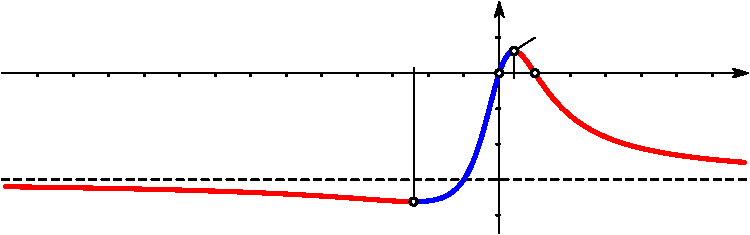
\includegraphics{05rationalexample.pdf}}
        \put( 18.05,  79.71){\sffamily\itshape \makebox[0pt][l]{{\tiny\sffamily\upshape -13}}}
    \put( 35.10,  79.71){\sffamily\itshape \makebox[0pt][l]{{\tiny\sffamily\upshape -12}}}
    \put( 52.14,  79.71){\sffamily\itshape \makebox[0pt][l]{{\tiny\sffamily\upshape -11}}}
    \put( 69.19,  79.71){\sffamily\itshape \makebox[0pt][l]{{\tiny\sffamily\upshape -10}}}
    \put( 86.24,  79.71){\sffamily\itshape \makebox[0pt][l]{{\tiny\sffamily\upshape -9}}}
    \put(103.29,  79.71){\sffamily\itshape \makebox[0pt][l]{{\tiny\sffamily\upshape -8}}}
    \put(120.33,  79.71){\sffamily\itshape \makebox[0pt][l]{{\tiny\sffamily\upshape -7}}}
    \put(137.38,  79.71){\sffamily\itshape \makebox[0pt][l]{{\tiny\sffamily\upshape -6}}}
    \put(154.43,  79.71){\sffamily\itshape \makebox[0pt][l]{{\tiny\sffamily\upshape -5}}}
    \put(171.48,  79.71){\sffamily\itshape \makebox[0pt][l]{{\tiny\sffamily\upshape -4}}}
    \put(188.52,  79.71){\sffamily\itshape \makebox[0pt][l]{{\tiny\sffamily\upshape -3}}}
    \put(205.57,  79.71){\sffamily\itshape \makebox[0pt][l]{{\tiny\sffamily\upshape -2}}}
    \put(222.62,  79.71){\sffamily\itshape \makebox[0pt][l]{{\tiny\sffamily\upshape -1}}}
    \put(256.71,  79.71){\sffamily\itshape \makebox[0pt][l]{{\tiny\sffamily\upshape 1}}}
    \put(273.76,  79.71){\sffamily\itshape \makebox[0pt][l]{{\tiny\sffamily\upshape 2}}}
    \put(290.81,  79.71){\sffamily\itshape \makebox[0pt][l]{{\tiny\sffamily\upshape 3}}}
    \put(307.86,  79.71){\sffamily\itshape \makebox[0pt][l]{{\tiny\sffamily\upshape 4}}}
    \put(324.90,  79.71){\sffamily\itshape \makebox[0pt][l]{{\tiny\sffamily\upshape 5}}}
    \put(341.95,  79.71){\sffamily\itshape \makebox[0pt][l]{{\tiny\sffamily\upshape 6}}}
    \put(243.67,   9.52){\sffamily\itshape \makebox[0pt][c]{{\tiny\sffamily\upshape -4}}}
    \put(243.67,  26.57){\sffamily\itshape \makebox[0pt][c]{{\tiny\sffamily\upshape -3}}}
    \put(243.67,  43.62){\sffamily\itshape \makebox[0pt][c]{{\tiny\sffamily\upshape -2}}}
    \put(243.67,  60.67){\sffamily\itshape \makebox[0pt][c]{{\tiny\sffamily\upshape -1}}}
    \put(243.67,  94.76){\sffamily\itshape \makebox[0pt][c]{{\tiny\sffamily\upshape 1}}}
    \put(180.51,   3.98){\sffamily\itshape abs.~min.}
    \put(258.71,  96.76){\sffamily\itshape abs.~max.}
    \put(195.51,  79.71){\sffamily\itshape $A$}
    \put(243.73,  67.71){\sffamily\itshape $B$}
\end{picture}

  \caption{The graph of $f(x) = 3(x-x^2)/(1+x^2)$}
  \label{fig:05rationalexample}
\end{figure}

Since we are dealing with an unbounded interval we must compute the limits of
$f(x)$ as $x\to\pm\infty$.  We find
\[
\lim_{x\to\infty} f(x) = \lim_{x\to-\infty} f(x) = -3.
\]
Since $f$ is decreasing between $-\infty$ and $A$, it follows that
\[
f(A) \leq f(x) < - 3 \text{ for } -\infty<x\leq A.
\]
Similarly, $f$ is decreasing from $B$ to $+\infty$, so
\[
-3 < f(x) \leq f(B) \text{ for } B < x<\infty.
\]
Between the two stationary points the function is increasing, so
\[
f(A) \leq f(x) \leq f(B) \text{ for } A\leq x\leq B.
\]
From this it follows that $f(x)$ has a global minimum when $x=A=-1-\sqrt{2}$
and has a global maximum when $x=B=-1+\sqrt{2}$.












\section{Convexity, Concavity and the Second Derivative} %{{{1

\subsection{Definition} %{{{2
\itshape A function $f$ is \emph{convex} on some interval
$a<x<b$ if the derivative $f'(x)$ is \emph{increasing} on that interval.




Likewise, the function is called \emph{concave} for $a<x<b$ if the derivative
$f'(x)$ is \emph{decreasing} on that interval.








\upshape\smallskip




In the following drawings the graph on the left is convex, while
\begin{figure}[h]\centering
  \parbox{115pt}{\input ../figures/221/05increasingtangent.tex }
  \parbox{115pt}{\input ../figures/221/05decreasingtangent.tex }
  \parbox{115pt}{\input ../figures/221/05inflectionpoint.tex }
  \caption{\textbf{Convex, concave and mixed graphs.}}
  \label{fig:05concave-convex-examples}
\end{figure}
the one in the middle is concave, because, going from left to right along either of
these graphs (from $A$ to $B$ to $C$ to $D$), you see that the slope of the
tangent increases on the left graph, and decreases on the middle graph.
The third graph is neither convex nor concave, although it does have one concave
piece and one convex piece.

By our results on increasing and decreasing functions, we know that $f$ is
convex if the derivative of $f'(x)$ is positive. In other words, if $f''(x)>0$
for $a<x<b$, then $f'(x)$ is increasing and therefore, by definition, $f(x)$ is
convex.


\subsection{Theorem (convexity and concavity from the second derivative)} %{{{2
\itshape If $f''(x)$ is positive for $a<x<b$, then the function $f$ is convex on
the interval $a<x<b$.

If $f''(x)$ is negative for $a<x<b$, then the function $f$ is concave on that
interval.\upshape\smallskip



\subsection{Definition} %{{{2
\itshape%
A point on the graph of $f$ where $f''(x)$ changes sign is called an
\emph{inflection point}.\upshape\smallskip

The third graph in Figure~\ref{fig:05concave-convex-examples} shows an inflection
point.

\subsection{The chords of convex graphs} %{{{2
Along the graph of a convex function the slope of the tangent is increasing as
you go from left to right.  After you try to draw a couple of such graphs it
really looks like they should always be ``curved upwards.''   The intuitive
understanding of convex and concave is that convex graphs are curved up, and
concave graphs are curved down.

The phrase ``curved upwards'' turns out to be another one of those expressions
whose mathematical definition is not clear (try explaining it with out waving
your hands.)  The following theorem is an attempt to make a more precise
statement that essentially says the graph is curved upwards.

\subsection*{Theorem} %{{{2
\itshape If a function $f$ is convex on some interval
$a<x<b$ then the chord connecting any two points on the graph lies
above the graph.  \upshape\smallskip


While this theorem is still phrased in terms of the picture, the condition that
``the chord lies above the graph'' can be expressed as an inequality between the
function $f(x)$ itself, and the function whose graph is the chord%
\footnote{The precise statement is: a function is convex on the interval $[a,b]$
if, for any $t$ with $0\leq t\leq 1$, and any $c$ and $d$ with $a\leq c < d\leq
b$, it is true that
\[
f(tc+(1-t)d) \leq t \,f(c) + (1-t)\, f(d).
\]
}.
To prove this theorem requires invoking the Mean Value Theorem.
  


\marginpar{\footnotesize\sffamily\itshape\centering
\input ../figures/221/05convexgraphwithchord.pdf_tex \\
The chord connecting $C$ and $D$ lies above the graph.}




\subsection{Example -- the cubic function $f(x) = x^3-3x$} %{{{2
\label{sec:convexpartofcubic}%
The second derivative of the function $f(x) = x^3-3x$ is
\[
f''(x) = 6x
\]
which is positive for $x>0$ and negative for $x<0$. Hence, in the graph in
\S\ref{sec:cubicgraph}, the origin is an inflection point, and the piece of the
graph where $x>0$ is convex, while the piece where $x<0$ is concave.


\subsection{The Second Derivative Test} %{{{2
In \S\ref{sec:isitamaxormin} we saw how you can tell if a stationary point is a
local maximum or minimum by looking at the sign changes of $f'(x)$.  There is
another way of distinguishing between local maxima and minima which involves
computing the second derivative.
\begin{theorem}
  Suppose $c$ is a stationary point for a function $f$.  If $f''(c)<0$, then $f$
  has a local maximum at $x=c$, and if $f''(c)>0$, then $f$ has a local minimum at $c$.
\end{theorem}\smallskip

The theorem doesn't say anything about what happens when $f''(c) = 0$.  To
determine what happens in that case, one must go back to checking the sign of
the first derivative near the stationary point.




The basic reason why this theorem is true is that if $c$ is a stationary point
with $f''(c)>0$, then we know that $f'(x)$ is increasing near $x=c$. But this is
only possible if $f'(x)<0$ for $x<c$ and $f'(x)>0$ for $x>c$ (in some small
interval around $c$).  This means the function $f$ is decreasing for $x<c$ and
increasing for $x>c$, which means it reaches a local minimum at $x=c$. An
analogous argument applies for the $f''(c)<0$ case.
\marginpar{\sffamily\itshape\footnotesize%
  \input ../figures/221/05concave-means-max.pdf_tex \\
  \input ../figures/221/05convex-means-min.pdf_tex }

\subsection{Example -- $f(x) = x^3-3x$, again} %{{{2
Consider the function $f(x) = x^3-3x$ from \S\ref{sec:cubicgraph} and
\S\ref{sec:convexpartofcubic}.  We found that this function has two
stationary points, at $x=\pm1$.  By looking at the sign of
$f'(x) = 3x^2-3$ we concluded that $x=-1$ is a local maximum while
$x=+1$ is a local minimum.
  
Instead of looking at $f'(x)$, we could also have computed $f''(x)$ at $x=\pm1$
and then applied the Second Derivative Test: since $f''(x) = 6x$, we have
\[
f''(-1) = -6 < 0 \text{ and }
f''(+1) = 6 > 0.
\]
Therefore $f$ has a local maximum at $-1$ and a local minimum at $+1$.




\begin{figure}[h]
  \centering 
    \begin{picture} (280.000000,81.428571)(0,0)
    \put(0.0, 0.0){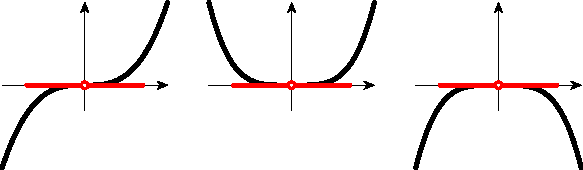
\includegraphics{05nonMorsepoints.pdf}}
        \put( 48.66,  72.49){\sffamily\itshape $y=x^3$}
    \put(147.94,  72.49){\sffamily\itshape $y=x^4$}
    \put(247.23,  72.49){\sffamily\itshape $y=-x^4$}
    \put( 40.71,  16.80){\sffamily\itshape \makebox[0pt][c]{%
\parbox{60pt}{\centering%
neither min\\ nor max}}}
    \put(140.00,  16.80){\sffamily\itshape \makebox[0pt][c]{local min}}
    \put(239.29,  16.80){\sffamily\itshape \makebox[0pt][c]{local max}}
\end{picture}

  \caption{Three functions for which the second derivative test
    doesn't work.}
  \label{fig:05nonMorsepoints}
\end{figure}




\subsection{When the second derivative test doesn't work} %{{{2
Usually the second derivative test will work, but sometimes a
stationary point $c$ has $f''(c)=0$.  In this case the second
derivative test gives no information at all.
Figure~\ref{fig:05nonMorsepoints} shows you the graphs of three
functions, all three of which have a stationary point at $x=0$.  In
all three cases the second derivative vanishes at $x=0$ so the second
derivative test says nothing.  As you can see, the stationary point
can be a local maximum, a local minimum, or neither.








\section{Problems} %{{{1
\problemfont %{{{3
\begin{multicols}{2}\setlength{\parindent}{0pt}




\problem What does the Intermediate Value Theorem say? %{{{3




\problem What does the Mean Value Theorem say? %{{{3

\problem  \textit{Rolle's Theorem} says that there is a stationary %{{{3
point between any pair of zeros of a function.  More precisely,
\begin{center}
  \rmfamily\itshape If $f(a) = 0$ and $f(b)=0$ then there is a $c$
  between $a$ and $b$ such that $f'(c) = 0$.
\end{center}
Show that this follows from the Mean Value Theorem. (Hint: It's a special case
of the Mean Value Theorem.  You can mimic the proof that was given in the text.)


\problem What is a stationary point? %{{{3




\problem \groupproblem How can you tell if a local maximum is a global %{{{3
maximum?




\problem \groupproblem If $f''(a) = 0$ then the graph of $f$ has an %{{{3
inflection point at $x=a$.  \emph{True or False?}
\answer %{{{3
Not necessarily true, and therefore false.  Consider the example
$f(x)=x^4$, and see the next problem.
\endanswer




\problem What is an inflection point? %{{{3
\answer %{{{3
An inflection point is a point on the graph of a function where the
second derivative changes its sign.  At such a point you must have
$f''(x) = 0$, but by itself that it is no enough.
\endanswer




\problem Give an example of a function for which $f'(0)=0$ even though the %{{{3
function $f$ has neither a local maximum or a local minimum at $x=0$.




\problem \groupproblem Draw four graphs of functions, one for each of %{{{3
the following four combinations:
\begin{align*}
  &f'>0\text{ and } f''>0 \\   &f'>0\text{ and } f''<0 \\
  &f'<0\text{ and } f''>0 \\   &f'<0\text{ and } f''<0 \\
\end{align*}

\problem \groupproblem Which of the following combinations are possible? %{{{3
\begin{align*}
  \textbf{(a)~}& f'(x)>0 \text{ and } f''(x)=0 \text{ for all } x \\
  \textbf{(b)~}& f'(x)=0 \text{ and } f''(x)>0 \text{ for all } x
\end{align*}
\answer %{{{3
The first is possible, e.g.~$f(x) = x$ satisfies $f'(x)>0$ and
$f''(x)=0$ for all $x$.

The second is impossible, since $f''$ is the derivative of
$f'$, so $f'(x) = 0$ for all $x$ implies that
$f''(x)=0$ for all $x$.
\endanswer








\bigskip




For each of the following functions, decide if they are
increasing, decreasing, or neither on the indicated intervals:

\problem $\displaystyle f(x) = \frac{x}{1+x^2} \text{, on }  10<x<\infty$ %{{{3

\problem $\displaystyle f(x) = \frac{2+x^2}{x^3-x} \text{, on }  1<x<\infty$ %{{{3

\problem $\displaystyle f(x) = \frac{2+x^2}{x^3-x} \text{, on }  0<x<1$ %{{{3

\problem $\displaystyle f(x) = \frac{2+x^2}{x^3-x} \text{, on }  0<x<\infty$ %{{{3

\bigskip

\textbf{Sketch the graphs} of the following functions.
You should
\begin{list}{--}{
    \setlength{\itemindent}{0pt}
    \setlength{\leftmargin}{6pt}}
\item find where $f$, $f'$ and $f''$ are positive or negative
\item find all stationary points and classify them as local minima, maxima, or neither
\item find any global maxima or minima, if they exist
\item find all inflection points
\item determine all intervals where the function is increasing or decreasing
\item determine all intervals where the function is convex or concave
\item find any horizontal, vertical, or slant asymptotes
\end{list}
















\problem $\displaystyle y=x^3+2x^2 $ %{{{3
\answer %{{{3
$y=0$ at $x=-1, 0, 0$.  Only sign change at $x=-1$, not at $x=0$.

$x=0$ loc min;  $x=-\frac43$ loc max;  $x=-2/3$ inflection point.
No global max or min.
\endanswer




\problem $\displaystyle y=x^3-4x^2$ %{{{3
\answer %{{{3
zero at $x=0, 4$; sign change at $x=4$; loc min at $x=\frac83$; loc
max at $x=0$; inflection point at $x=4/3$.  No global max or min.
\endanswer




\problem $\displaystyle y=x^4+27x $ %{{{3
\answer %{{{3
sign changes at $x=0, -3$;  global min at $x=-3/4^{1/3}$; no inflection
points, the graph is convex.
\endanswer




\problem $\displaystyle y=x^4-27x$ %{{{3
\answer %{{{3
mirror image of previous problem.
\endanswer




\problem $\displaystyle y=x^4+2x^2-3 $ %{{{3
\answer %{{{3
$x^4+2x^2-3 = \bigl(x^2-1\bigr)\bigl(x^2+3\bigr)$ so sign changes at
$x=\pm1$.  Global min at $x=0$;  graph is convex, no inflection points.
\endanswer




\problem $\displaystyle y=x^4-5x^2+4 $ %{{{3
\answer %{{{3
Sign changes at $\pm2, \pm1$;  \emph{two} global minima, at $\pm\sqrt{5/2}$;
one local max at x=0;  two inflection points, at $x=\pm\sqrt{5/6}$.
\endanswer




\problem $\displaystyle y=x^5+16x$ %{{{3
\answer %{{{3
Sign change at $x=0$;  function is always increasing so no stationary
points;  inflection point at $x=0$.
\endanswer




\problem $\displaystyle y=x^5-16x$ %{{{3
\answer %{{{3
sign change at $x=0, \pm 2$;  loc max at $x=2/5^{1/4}$; loc min at
$x=-2/5^{1/4}$. Inflection point at $x=0$.
\endanswer




\problem $\displaystyle y=\frac{x} {x+1}$ %{{{3
\answer %{{{3
Function not defined at $x=-1$.  For $x>-1$ sign change at $x=0$, no
stationary points, no inflection points (graph is concave).
Horizontal asymptote $\lim_{x\to \infty}f(x) = 1$.




For $x<-1$ no sign change , function is increasing and convex, horizontal
asymptote with $\lim_{x\to-\infty}f(x) = 1$.
\endanswer




\problem $\displaystyle y=\frac{x}{1+x^2}$ %{{{3
\answer %{{{3
global max (min) at $x=1$ (x=-1), inflection points at $x=\pm\surd3$;
horizontal asymptotes $\lim_{x\to \pm\infty}f(x) = 0$.
\endanswer




\problem $\displaystyle y=\frac{x^2}{1+x^2}$ %{{{3
\answer %{{{3
$y=0$ at $x=0$ but no sign changes anywhere;  $x=0$ is a global min;
there's no local or global max;  two inflection points at
$x=\pm\frac13\surd3$; horizontal asymptotes at height $y=1$.
\endanswer




\problem $\displaystyle y=\frac{1+x^2}{1+x}$ %{{{3
\answer %{{{3
Not defined at $x=-1$.  For $x>-1$ the graph is convex and has a
minimum at $x=-1+\surd2$;  for $x<-1$ the graph is concave with a
maximum at $x=-1-\surd2$.  No horizontal asymptotes.
\endanswer




\problem $\displaystyle y=x+\frac1x$ %{{{3
\answer %{{{3
Not def'd at $x=0$. No sign changes (except at $x=0$).
For $x>0$ convex with minimum at $x=1$, for $x<0$ concave
with maximum at $x=-1$.
\endanswer




\problem $\displaystyle y=x-\frac1x$ %{{{3
\answer %{{{3
Not def'd at $x=0$. Sign changes at $x=\pm1$ and also at $x=0$.
No stationary points.  Both branches ($x>0$ and $x<0$) are
increasing.  Non inflection points, no horizontal asymptotes.
\endanswer




\problem $\displaystyle y=x^3+2x^2+x$ %{{{3
\answer %{{{3
Zero at $x=0, -1 $ sign only changes at $-1$;  loc min at
$x=-\frac13$; loc max at $x=-1$.  Inflection point at $x=-2/3$.
\endanswer




\problem $\displaystyle y=x^3+2x^2-x$ %{{{3
\answer %{{{3
Changes sign at $x=-1\pm\surd2$ and $x=0$; loc min at
$(-2+\surd7)/3$, loc max at $(-2-\surd7)/3$; inflection point at
$x=-\frac23$.
\endanswer




\problem $\displaystyle y=x^4-x^3-x$ %{{{3
\answer %{{{3
Factor $y=x^4-x^3-x=x(x^3-x^2-1)$.  One zero is obvious, namely
at $x=0$.  For the other(s) you must solve $x^3-x^2-1=0$ which is
beyond what's expected in this course.\\
The derivative is $y'=4x^3-3x^2-1$.  A cubic function whose
coefficients add up to 0 so $x=1$ is a root, and you can factor
$y'=4x^3-3x^2-1= (x-1)(4x^2+x+1)$ from which you see that $x=1$
is the only root.  So: one stationary point at $x=1$, which is a
global minimum\\
The second derivative is $y''=12x^2-6x$; there are two inflection
points, at $x=\frac12$ and at $x=0$.
\endanswer




\problem $\displaystyle y=x^4-2x^3+2x$ %{{{3
\answer %{{{3
Again one obvious solution to $y=0$, namely $x=0$.  The other
require solving a cubic equation.\\ The derivative is
$y'=4x^3-6x^2+2$ which is also cubic, but the coefficients add up to
0, so $x=1$ is a root.  You can then factor
$y'=4x^3-6x^2+2=(x-1)(4x^2-2x-2)$.  There are three stationary
points: local minima at $x=1$, $x=-\frac14 - \frac12\surd3$, local
max at $x=-\frac14 + \frac12\surd3$.  One of the two loc min is a
global minimum.
\endanswer




\problem $\displaystyle y=\sqrt{1+x^2}$ %{{{3
\answer %{{{3
Global min at $x=0$, no other stationary points;  function is
convex, no inflection points.  No horizontal asymptotes.
\endanswer




\problem $\displaystyle y=\sqrt{1-x^2}$ %{{{3
\answer %{{{3
The graph is the upper half of the unit circle.
\endanswer




\problem $\displaystyle y=\sqrt[4]{1+x^2}$ %{{{3
\answer %{{{3
Always positive, so no sign changes;  global minimum at $x=0$, no
other stationary points; two inflection points at $\pm\surd2$.  No
horizontal asymptotes since $\lim_{x\to\pm\infty} \sqrt[4]{1+x^2} =
\infty \textrm{(DNE)}$.
\endanswer




\problem $\displaystyle y=\frac1{1+x^4} $ %{{{3
\answer %{{{3
Always positive hence no sign changes; global max at $x=0$, no other
stationary points;  two inflection points at $x=\pm\sqrt[4]{3/5}$;
second derivative also vanishes at $x=0$ but this is not an
inflection point.
\endanswer








\bigskip
\noindent%
The following functions are \textbf{periodic}, meaning that they satisfy $f(x+L)=f(x)$ for
  all $x$ and a constant $L$ called the \textbf{period} of the function.  The
graph of a periodic function repeats itself indefinitely to the left and to
the right.  It therefore has infinitely many (local) minima and maxima, and
infinitely many inflection points.  Sketch the graphs of the following
functions as in the previous problem, but only list those ``interesting
points'' that lie in the interval $0\leq x<2\pi$.




\problem $\displaystyle y=\sin x$ %{{{3




\problem $\displaystyle y=\sin x+\cos x$ %{{{3
\answer %{{{3
Zeroes at $x=3\pi/4$, $7\pi/4$. Absolute max at $x=\pi/4$, abs min at
$x=5\pi/4$.  Inflection points and zeroes coincide.  Note that
$\sin x+\cos x = \sqrt2 \sin(x+\frac\pi4)$.
\endanswer




\problem $\displaystyle y=\sin x +\sin^2 x$ %{{{3
\answer %{{{3
Zeroes at $x=0, \pi, 3\pi/2$ but no sign change at $3\pi/2$.  Global
max at $x=\pi/2$, local max at $x=3\pi/2$, global min at $x=7\pi/6,
11\pi/6$.
\endanswer




\problem $\displaystyle y=2\sin x+\sin^2x$ %{{{3




\problem $\displaystyle y=4\sin x +\sin^2 x$ %{{{3




\problem $\displaystyle y=2\cos x+\cos^2x$ %{{{3




\problem $\displaystyle y=\frac4{2+\sin x}$ %{{{3




\problem $\displaystyle y=\bigl(2+\sin x\bigr)^2$ %{{{3












\bigskip








\textbf{Graphing inverse trigonometric functions. }
Find the domains and sketch the graphs of each of the following functions




\problem $\displaystyle y=\arcsin x$ %{{{3




\problem $\displaystyle y=\arctan x$ %{{{3




\problem $\displaystyle y=2\arctan x-x$ %{{{3




\problem $\displaystyle y=\arctan(x^2)$ %{{{3




\problem $\displaystyle y=3\arcsin(x) - 5x $ %{{{3




\problem $\displaystyle y=6\arcsin (x) - 10x^2$ %{{{3












\bigskip


\problem Sometimes we will have functions for which we cannot solve $f'(x)=0$, %{{{3
but will still allow us to say something using the derivative.




\subprob Show that the function $f(x) = x\arctan x$ is convex.  Then
sketch the graph of $f$.




\subprob Show that the function $g(x) = x\arcsin x$ is convex.  Then
sketch the graph of $g$.


\problem  Let $\frac pq$ be some fraction, with $p>0$, $q>0$. %{{{3
Assume also that $p<q$ so that the fraction is less than 1.

If you increase both numerator $p$ and denominator $q$ by the same amount
$x>0$, does the fraction increase or decrease?  In other words, which of the
following two inequalities holds:
\[
  \frac{p+x}{q+x} > \frac{p}{q}
  \text{ or }
  \frac{p+x}{q+x} < \frac{p}{q}?
\]
Explain how you can answer this question by checking that a certain
function is increasing or decreasing.  Which function would you look
at?

How does your answer change if $p>q$?




\problem\subprob Consider the list of numbers %{{{3
\[
\tfrac{1} {2},\,
\tfrac{2} {5},\,
\tfrac{3} {10},\,
\tfrac{4} {17},\,
\tfrac{5} {26},\,
\cdots.
\]
The $n$th number in the list is
\[
a_n = \frac{n} {n^2+1}.
\]
Is it true that each number in the list is less than its predecessor?  I.e., is
it true that
\[
a_{n+1} < a_n
\]
for all $n=1, 2, 3, 4, \ldots$?




\subprob Consider the following list of numbers
\[
\tfrac{1} {2},\,
\tfrac{2} {3},\,
\tfrac{3} {6},\,
\tfrac{4} {11},\,
\tfrac{5} {18},\,
\cdots,
\]
where the $n$th number in the list is
\[
a_n = \frac{n} {n^2-2n+3}.
\]
For which $n$ is $a_{n+1} < a_n$?




\problem  \label{ex:implicit-from-ch1} %{{{3
Show that the equation $3y+\sin y = \frac\pi2$ has exactly
one solution $y$.  (In chapter I,~\S\ref{sec:why-implicit} we had agreed to
check this.)
\end{multicols}
\noproblemfont


%%% This section should be called "optimization problem" since there is only one example in it!
\section{Applied Optimization} %{{{1
Many problems, after some amount of work, can be rephrased as
\begin{center}
  \textit{For which value of $x$ in the interval $a\leq x\leq b$ is $f(x)$ the
    largest?}
\end{center}
In other words, given a function $f$ on an interval $[a, b]$, we want to determine the maximum value of $f$ on this interval (and usually, for what values of $x$ the function attains its maximum value).




If the function is continuous, then according to theorem \ref{thm:max-min-exist}
there always is at least one $x$ in the interval $[a,b]$ which maximizes $f(x)$.




If $f$ is differentiable then we know that any local maximum is either a
stationary point or one of the end points $a$ and $b$.  Therefore, we can find
the global maxima by following this recipe:
\begin{enumerate}\sffamily\itshape
\item Find all stationary points of $f$;
\item Compute $f(x)$ at each stationary point from step (1);
\item Compute $f(a)$ and $f(b)$;
\item Compare all of the computed values from steps (2) and (3), and pick the biggest one.
\end{enumerate}
Note that there is a single global maximum value on any interval $[a,b]$, although it may occur at more than one $x$-value in that interval.




The same procedure holds for looking for global minima, in order to
\textit{minimize} rather than \textit{maximize} a function.  The same procedure
works, except of course in step (4) we want to find the smallest value rather
than the biggest one.




The difficulty in optimization problems frequently lies not with the calculus
part, but rather with setting up the problem.  Choosing which quantity to call
$x$ and finding the function $f$ is half the job.


\subsection{Example -- The rectangle with largest area and given perimeter} %{{{2
Which rectangle has the largest area, among all those rectangles for which the
total length of the sides is $1$?

\textit{Solution: } If the sides of the rectangle have lengths $x$ and $y$, then
the total length of the sides is
\[
L = x+x+y+y = 2(x+y)
\]
and the area of the rectangle is
\[
A = xy.
\]
So we are asked to find the largest possible value of $A=xy$ provided
$2(x+y)=1$.  The lengths of the sides can also not be negative, so $x$
and $y$ must satisfy $x\geq0$, $y\geq0$.

We now want to turn this problem into a question of the form ``maximize a
function over some interval''.  The quantity which we are asked to maximize is
$A$, but it depends on two variables $x$ and $y$ instead of just one variable.
However, the variables $x$ and $y$ are not independent since we are only allowed
to consider rectangles with $L=1$.  From this equation we get
\[
L=1\implies y = \tfrac12-x.
\]
Hence we must find the maximum of the quantity
\[
A= xy = x\bigl(\tfrac12-x\bigr)
\]
The values of $x$ which we are allowed to consider are only limited by
the requirements $x\geq 0$ and $y\geq0$, i.e.\ $x\leq \tfrac12$.  So
we end up with this problem:
\begin{center}
  \textit{Find the maximum of the function
    $f(x)=x\bigl(\tfrac12-x\bigr)$ on the interval $0\leq x\leq
    \tfrac12$.}
\end{center}
Before we start computing anything we note that the function $f$ is a
polynomial so that it is differentiable, and hence continuous, and
also that the interval $0\leq x\leq\tfrac12$ is closed.  Therefore the
theory guarantees that there is a maximum and our recipe will show us
where it is.

The derivative is given by
\[
f'(x) = \tfrac12 - 2x,
\]
and hence the only stationary point is \( x=\tfrac14 \).  The function value at
this point is
\[
f\tfrac14) = \tfrac14(\tfrac12-\tfrac14) = \tfrac1{16}.
\]
At the endpoints one has $x=0$ or $x=\tfrac12$, which corresponds to a rectangle
one of whose sides has length zero.  The area of such rectangles is zero, and so
this is not the maximal value we are looking for.

We conclude that the largest area is attained by the rectangle whose sides have
lengths
\[
x=\tfrac14, \text{ and }y= \tfrac12-\tfrac14 = \tfrac14,
\]
which is a square with sides of length $\tfrac14$.


\section{Problems} %{{{1
\problemfont %{{{3
\begin{multicols}{2}\setlength{\parindent}{0pt}
% deleted problem 99% identical to the example in the section


\problem Which rectangle of area 100in$^2$ minimizes its height plus %{{{3
two times its length?
\answer %{{{3
If the sides are $x$ and $y$, then the area is $xy = 100$, so $y=1/x$.
Therefore the height plus twice the width is $f(x) = x+2y = x+2/x$.
This is extremal when $f'(x) = 0$, i.e.\ when $f'(x) = 1-2/x^2 = 0$.
This happens for $x=\sqrt2$.
\endanswer






% !!! TO-DO: include a picture of this problem!
\problem You have 1 yard of string from which you make a circular %{{{3
wedge with radius $R$ and opening angle $ \theta$.  Which choice of $
\theta$ and $R$ will give you the wedge with the largest area?  Which
choice leads to the smallest area?

[A circular wedge is the figure consisting of two radii of a circle
and the arc connecting them.  So the yard of string is used to form
the two radii and the arc.]
\answer %{{{3
Perimeter is $2R+R\theta = 1$ (given), so if you choose the angle to
be $\theta$ then the radius is $R=1/(2+\theta)$.  The area is then
$A(\theta) = \theta R^2 = \theta/(2+\theta)^2$, which is maximal when
$\theta=2$ (radians).  The smallest area arises when you choose
$\theta=0$.  Choosing $\theta\ge 2\pi$ doesn't make sense (why?  Draw
the corresponding wedge!)




You could also say that for any given radius $R>0$ ``perimeter
$=1$'' implies that one has $\theta = (1/R)-2$.  Hence the area
will be $A(R) =\theta R^2 = R^2\bigl( (1/R)-2 )\bigr) = R-2R^2$.  
Thus the area is maximal when $R=\frac14$, and hence
$\theta=2$radians.  Again we note that this answer is reasonable
because values of $\theta>2\pi$ don't make sense, but $\theta=2$
does.
\endanswer








\problem \groupproblem \textbf{(The lamp post problem)} %{{{3
In a street two lamp posts are 300 feet apart.  The light intensity at
a distance $d$ from the first lamp post is $1000/d^2$, the light
intensity at distance $d$ from the second (weaker) lamp post is
$125/d^2$ (in both cases the light intensity is inversely proportional
to the square of the distance to the light source).  




\centerline{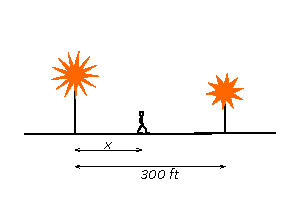
\includegraphics{05lamppost.pdf}}




The \textit{combined light intensity} is the sum of the two light
intensities coming from both lamp posts.




\subprob If you are in between the lamp posts, at distance $x$
feet from the stronger light, then give a formula for the combined light
intensity coming from both lamp posts as a function of $x$.




\subprob What is the darkest spot between the two lights, i.e.\
where is the combined light intensity the smallest?




\answer %{{{3
\textbf{(a)} The intensity at $x$ is a function of $x$.  Let's
call it $I(x)$.  Then at $x$ the distance to the big light is
$x$, and the distance to the smaller light is $1000-x$. Therefore
\[
  I(x) = \frac{1000}{x^2} + \frac{125}{(1000-x)^2}
\]
\textbf{(b)} Find the minimum of $I(x)$ for $0<x<1000$.
\[
  I'(x) = -2000 x^{-3} + 250(1000 - x)^{-3}.
\]
$I'(x) = 0$ has one solution, namely, $x= \frac{1000}{3}$.
By looking at the signs of $I'(x)$ you see that $I(x)$ must have a
minimum.  If you don't like looking at signs, you could instead
look at the second derivative
\[
  I''(x) = 6000 x^{-4} + 750 (1000 - x)^{-4}
\]
which is always positive.
\endanswer








\problem  %biggest soup can %{{{3
\subprob You have a sheet of metal with area $100\text{ in}^2$
from which you are to make a cylindrical soup can (with both a top and a bottom).  If $r$ is the
radius of the can and $h$ its height, then which $h$ and $r$ will
give you the can with the largest volume?
\answer %{{{3
The soup can is made of two disks (the top and bottom) and the side.
Both top and bottom have area $\pi r^2$.
The side can be made by bending a rectangular piece of metal into
a cylinder.  The sides of the rectangular piece of metal needed for
this are $h$ (height of the cylinder) and $2\pi r$ (perimeter of
the cylinder).  Therefore the total area of the metal that is needed
to make a cylinder of height $h$ and radius $r$ is
\[
A = 2\pi r^2 + 2\pi rh = 100 \mathsf{in}^2.
\]
The volume of that cylinder is
\[
V = \text{area base} \times \text{height} = \pi r^2h.
\]
We have to choose which variable we use to distinguish the different
sizes of cans that we can make.  The variables at hand are $r$
and $h$.  If we choose $h$ then we would have to get rid of $r$,
which involves solving the equation $A=100$ for $r$.  That equation
is quadratic, and formula for $r$ will involve square roots.




The other choice is the variable $r$.  Then we have to eliminate $h$,
i.e.~solve $A=100$ for $h$.  The solution is
\[
2\pi r^2 + 2\pi rh = 100 \implies
h = \frac{100 - 2\pi r^2} {2\pi r}.
\]




\endanswer




\subprob If instead of making a plain cylinder you replaced the
flat top and bottom of the cylinder with two hemispherical caps, then
(using the same 100in$^2$ of sheet metal), then which choice of
radius and height of the cylinder give you the container with the
largest volume?




\subprob Suppose you only replace the top of the cylinder with a
hemispherical cap, and leave the bottom flat.  Then which choice of height
and radius of the cylinder result in the largest volume?




\answer %{{{3
\textbf{(a)} The optimal radius is $r = \sqrt{50/3\pi}$, and the corresponding
height is $h = 100/(3\pi r) = 100/\sqrt{150\pi}$.
\endanswer





\problem A triangle has one vertex at the origin $O(0,0)$, another at the %{{{3
point $A(2a,0)$ and the third at $(a, a/(1+a^3))$.  What are the largest
and smallest areas this triangle can have if $0\leq a<\infty$?

\problem \groupproblem \textit{(Queen Dido's problem)} %{{{3

According to tradition Dido was the founder and first Queen of
Carthage.  When she arrived on the north coast of Africa
($\sim$800BC) the locals allowed her to take as much land as could be
enclosed with the hide of one ox.  She cut the hide into thin strips
and put these together to form a length of 100 yards\footnote{I made
that number up.  For the rest start at
\url{http://en.wikipedia.org/wiki/Dido}}.


    \begin{picture} (180.000000,48.725000)(0,0)
    \put(0.0, 0.0){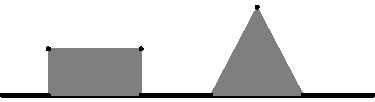
\includegraphics{05dido.pdf}}
        \put( 15.25,   6.22){\sffamily\itshape $A$}
    \put( 15.25,  28.48){\sffamily\itshape $B$}
    \put( 70.75,  28.48){\sffamily\itshape $C$}
    \put( 70.75,   6.22){\sffamily\itshape $D$}
    \put( 95.12,   6.22){\sffamily\itshape $P$}
    \put(126.38,  48.50){\sffamily\itshape $Q$}
    \put(148.62,   6.22){\sffamily\itshape $R$}
    \put(167.88,   6.22){\sffamily\itshape land}
    \put(167.88,  -6.78){\sffamily\itshape water}
\end{picture}


\subprob \rule{0pt}{14pt} If Dido wanted a rectangular region,
then how wide should she choose it to enclose as much area as
possible (the coastal edge of the boundary doesn't count, so in this
problem the length $AB+BC+CD$ is 100 yards.)

\subprob If Dido chose a region in the shape of an isosceles
triangle $PQR$, then how wide should she make it to maximize its area
(again, don't include the coast in the perimeter: $PQ+QR$ is 100
yards long, and $PQ=QR$.)


\problem The product of two numbers $x, y$ is 16. We know $x\geq 1$ and $y %{{{3
\geq1$. What is the greatest possible sum of the two numbers?


\problem What are the smallest and largest values that $(\sin x)(\sin y)$ can %{{{3
have if  $x+y=\pi$ and if $x$ and $y$ are both nonnegative?


\problem What are the smallest and largest values that $(\cos x)(\cos y)$ can %{{{3
have if  $x+y=\frac\pi2$ and if $x$ and $y$ are both nonnegative?


\problem %max&min of tan x+tan y, with x+y=pi/2 %{{{3
\subprob  Find the smallest and largest values of $\tan x
+ \tan y$ can have if $x+y=\frac\pi2$ and if $x$ and $y$ are both
nonnegative?




\subprob
What are the smallest and largest values that $\tan x + 2\tan y$ can
have if  $x+y=\frac\pi2$ and if $x$ and $y$ are both nonnegative?





\problem If a locomotive is traveling at $v$ miles per hour, the cost per hour %{{{3
of fuel $v^2 /25$ dollars, and other costs are \$100 per hour regardless of
speed. What is the speed that minimizes cost \textbf{per mile}?

\problem \groupproblem Josh is in need of coffee.  He has a circular filter with %{{{3
3 inch radius.  He cuts out a wedge and glues the two edges $AC$ and $BC$
together to make a conical filter to hold the ground coffee.  The volume $V$ of
the coffee cone depends the angle $\theta$ of the piece of filter paper Josh
made.

\centerline{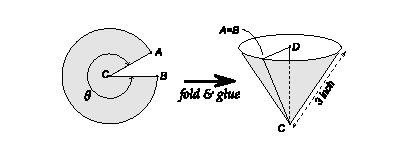
\includegraphics{05melita.pdf}}

\subprob  Find the volume in terms of the angle $\theta$.  (Hint:
how long is the  circular arc $AB$ on the left?  How long is the
circular top of the cone on the right?  If you know that you can find
the radius $AD=BD$ of the top of the cone, and also the height $CD$ of
the cone.)

\subprob Which angle $\theta$ maximizes the volume $V$?

\problem  Here are two equivalent problems (read both \& choose one): %{{{3

\subprob Blood pressure is the pressure exerted by circulating blood on
walls of the arteries. Assume the blood pressure varies periodically
according to the formula
\[
  p(t) = 50 +15\sin(2.5\pi t)
\]
where $t$ is the number of seconds since the beginning of a cardiac
cycle. When is the blood pressure the highest for $0 \leq t \leq 1$? What
is the maximum blood pressure? When is the blood pressure lowest in the
interval $0 \leq t \leq 1$ and what is the corresponding blood pressure?

\subprob The water level in a well is described as a function of time by
\[
  p(t) = 50 +15\sin(2.5\pi t).
\]
What is highest (resp.~smallest) water level in the time
interval $0 \leq t \leq 1$?








\problem A manufacturer needs to make a cylindrical can (with top and bottom) that will hold $1$ liter %{{{3
of liquid.  Determine the dimensions of the can that will minimize the amount of
material used in its construction.




\problem A window is being built in the shape of semicircle on the top of a %{{{3
rectangle, where there is a frame between the semicircle and rectangle as well
as around the boundary of the window. If there is a total of $15$ meters of
framing materials available, what must the dimensions of the window be to let in
the most light?

\problem A $5$ feet piece of wire is cut into two pieces. One piece is bent into %{{{3
a square and the other is bent into an equilateral triangle.  Where should the
wire be cut so that the total area enclosed by both figures is minimal?

\problem Two poles, one $5$ meters tall and one $10$ meters tall, are $20$ %{{{3
meters apart.  A telephone wire is attached to the top of each pole and it is
also staked to the ground somewhere between the two poles.

\subprob Where should the wire be staked so that the minimum amount of wire is
used?

\subprob Where should the wire be staked so that the angle formed by the two
pieces of wire at the stake is a maximum?


\problem Determine the cylinder with the largest volume that can be %{{{3
inscribed in a cone of height $10$ cm and base radius $6$ cm.



\problem A straight piece of wire $10$ feet long is bent into the shape of a %{{{3
right-angled $L$-shape. What is the shortest possible distance between the ends?

\problem An open-top cylindrical tank with a volume of $10$ cubic feet is to be %{{{3
made from a sheet of steel. Find the dimensions of the tank that will require as
little material used in the tank as possible.

\problem A box with a square base and open top must have a volume of $32,000$ %{{{3
  $\text{cm}^3$. Find the dimensions of the box that minimize the amount of material used
for building it.

\problem Find the length of the shortest ladder that will reach over an %{{{3
8-ft.~high fence to the wall of a tall building which is 3 ft.~behind the
fence.

\problem A rectangular piece of paper is 10 inches high and 6 inches %{{{3
wide. The lower right-hand corner is folded over so as to reach the
leftmost edge of the paper. Find the minimum length of the resulting
crease.




%%
%%\problem %{{{3
%%\begin{trivlist}
%%\item[(Bio)] The rate at which the body weight $y$ changes with respect to
%%  the age $x$ is proportional to $y^c$, for $c$ a species-specific positive
%%  constant. The relative growth rate defined as $\frac{1}{y} \cdot
%%  \frac{dy}{dx}$ measures the percentage weight gained per unit of
%%  time. For what values of $c$ is the relative growth rate increasing, and
%%  for which values it is decreasing?
%%\end{trivlist}
%%




%%\problem %{{{3
%%\begin{trivlist}
%%\item[(Bio)] The concentration of nitrogen in the soil is given by the
%%  function
%%  \[
%%  N(x)=(3-x)(4-x), \ \ \ 0 \leq x \leq 3
%%  \]
%%
%%  where $x$ is the depth in the soil where the measurement takes place.  At
%%  what depth from the soil surface is the concentration of nitrogen
%%  maximal?
%%\item[(Che)] The reaction rate of a chemical process is given by the
%%  function
%%  \[
%%  R(x)=(3-x)(4-x), \ \ \ 0 \leq x \leq 3
%%  \]
%%
%%  where $x$ is the concentration of the product resulted from the
%%  reaction. Find the concentration $x$ that maximizes the reaction rate.
%%
%%\item[(EMP)] A particle moving in the region of the plane given by $0 \leq
%%  x \leq 3$ follows a trajectory described by the equation
%%  $y(x)=x^2-7x+12$. Find the $x$-coordinate of the position of the particle
%%  corresponding to the highest $y$ coordinate.
%%\end{trivlist}
%%
\problem In the $xy$-plane, an observer stands at the origin $(0,0)$. A car %{{{3
travels along the curve $y=1/x^2$. How close does the car come to the observer?




%%\problem %{{{3
%%\begin{trivlist}
%%\item[(Bio)] The Pacific salmon can breed only once during its
%%  lifetime. The per capita rate of increase $r$ is a measure of
%%  reproductive fitness, in the sense that the greater $r$, the more
%%  offspring an individual produces. The rate of increase $r$ is a function
%%  of age $x$, given by
%%  \[
%%  r(x)=\frac{\ln[u(x)v(x)]}{x}
%%  \]
%%  where $u(x)$ is the probability of surviving to age $x$, and $v(x)$ is
%%  the number of female births at age $x$. Find the optimal age of
%%  reproduction, that is, the age $x$ that maximizes $r(x)$, if
%%  $u(x)=e^{-2x}$ and $v(x)=3x^2$.
%%\item[(EMP)] The efficiency of a technological process is measured by the
%%  function
%%  \[
%%  r(x)=\frac{\ln[3x^2e^{-2x}]}{x}
%%  \]
%%  where $x$ is the number of units produced. What number of units should be
%%  produced in order to maximize the efficiency function?
%%\end{trivlist}




%%\problem %{{{3
%%\begin{trivlist}
%%\item[(Bio)] The yield $y$ of an agricultural crop as a function of
%%  nitrogen level $x$ in the soil is modeled by the relationship
%%  \[
%%  y(x)=\frac{x}{1+x^2}, \ \ {\rm for} \ \ x \geq 0.
%%  \]
%%
%%  Find the nitrogen level that maximizes the yield.
%%\item[(Che)] The temperature $T$ in a certain chemical reaction varies as a
%%  function of time $t$ according to the rule
%%  \[
%%  T(t)=\frac{t}{1+t^2}.
%%  \]
%%  At what time during the reaction is the temperature at its maximal value?
%%\item[(EMP)] The pressure $P$ in a gas chamber varies as a function of time
%%  $t$ according to the rule
%%  \[
%%  P(t)=\frac{t}{1+t^2}.
%%  \]
%%  When is the pressure in the chamber at its highest value?
%%\end{trivlist}
%%
%%\problem ({\it van der Waals equation for real gases}) %{{{3
%%
%%The {\it ideal gas law} asserts that $PV=nRT$, where $P$ is the pressure
%%of the gas, $V$ is the gas volume, $n$ is the number of moles of gas, $T$
%%is the gas temperature, and $R$ is the ideal gas constant. However, the
%%ideal gas law does not hold at high pressures, and the {\it van der Waals
%%equation} for real gases
%%\[
%%  (P+\frac{n^2 a}{V^2})(V-nb)=nRT
%%\]
%%is used instead. The {\it van der Waals constants} $a$ and $b$ have been
%%determined experimentally for each gas. The {\it pressure deviation from
%%ideality}
%%\[
%%  P_{\rm dev}=P_{\rm real}-P_{\rm ideal}
%%\]
%%measures the difference in pressure as predicted by the ideal gas law, and,
%%respectively, van der Waals' law.
%%
%%$1.00$ mol of nitrogen N$_2$ is stored in a closed but flexible container
%%at a temperature of $300$ K.  What gas volume corresponds to the maximal
%%deviation from ideality $P_{\rm dev}$ if $R=0.08206$ $L \cdot
%%\textrm{atm}/\textrm{mol} \cdot
%%K$, $a=1.39$ $L^2 \cdot \textrm{atm}/\textrm{mol}^2$ and $b=0.0391$
%%$L/\textrm{mol}$?
\end{multicols}
\noproblemfont


\section{Parametrized Curves} %{{{1
\label{sec:05parametrized-curves-and-lHopital}
So far all the plane curves that we have seen were graphs of
functions $y=f(x)$.  A different way of describing a plane curve is to think of it as the
path that is traced out by a particle moving in the plane.  If you have a particle
that is moving about in the plane, then you can describe its motion by
specifying the coordinates $(x, y)$ of the point as functions of time: the
motion is given by two functions
\[
x = x(t), \quad y=y(t).
\]%
\marginpar{\input ../figures/221/05parametrized-curve.pdf_tex }%
As $t$ varies (``as time goes by'') the point $(x(t), y(t))$ traces out a curve.
This kind of curve is called a \emph{parametric curve} (or sometimes
\textit{parametrized curve}, or ``a curve defined by parametric equations'').
This topic reappears in third semester calculus (Math 234) where much of the
material can be simplified using vectors.




\subsection{Example: steady motion along a straight line} %{{{2
The simplest motion is where the particle moves with constant velocity.
Suppose the particle starts out at $(x_0, y_0)$ at time $t=0$, and
suppose its horizontal and vertical velocities are $v_x$ and $v_y$,
respectively.  Then after a time $t$ has gone by the point has moved a
distance $v_x t$ in the $x$-direction and $v_y t$ in the
$y$-direction.  Its coordinates are therefore
\begin{equation}
  x(t) = x_0 + v_x t, \quad
  y(t) = y_0 + v_y t.
  \label{eq:05motion-on-line}
\end{equation}
One question we can ask is: how fast is the particle moving?


\begin{figure}[h]
  \sffamily\small%
  \input ../figures/221/05motion-on-a-line.pdf_tex
  \caption{Motion with constant velocity along a straight line}
\end{figure}
We know that both its $x$-coordinate and $y$-coordinate increase at constant
rates $v_x$ and $v_y$.  So, between time $t$ and time $t+\Delta t$, the $x$ and
$y$ coordinates increase by $\Delta x = v_x \Delta t$ and $\Delta y =v_y \Delta
t$, so therefore the distance traveled by the point is
\begin{equation}
  \Delta s = \sqrt{(\Delta x)^2 + (\Delta y)^2} = t\,\sqrt{v_x^2 + v_y^2}.
  \label{eq:05distance-travelled-along-line}
\end{equation}
Then we can get the average speed $v$ by dividing by $\Delta t$:
\begin{equation}
  v = \frac{\Delta s} {\Delta t}
  = \sqrt{\Bigl(\frac{\Delta x}{\Delta t}\Bigr)^2
    + \Bigl(\frac{\Delta y}{\Delta t}\Bigr)^2}
  =\sqrt{v_x^2 + v_y^2}.
  \label{eq:velocity-along-line}
\end{equation}
Since the average speed turns out not to depend on the length $\Delta t$ of
the time interval, we see that the instantaneous speed at any time $t$
will also be equal to the value $v$ we have just found.


\begin{figure}[t]
  \small%
  \input ../figures/221/05motion-on-a-circle.pdf_tex
  \caption{\textbf{Constant velocity motion along a circle.}  The
    coordinates of any point on the circle with radius $R$ and center
    $(x_0,y_0)$ are completely determined by the angle $\theta$ (on
    the right).  To describe the motion of a particle on the circle you
    only have to specify how the angle $\theta$ changes with time.
    For a motion with constant angular velocity (on the left) $\theta$
    starts out at some value $\phi$ when $t=0$; after time $t$ the
    angle $\theta$ has increased by $\omega t$, and thus has the value
    $\theta = \phi+\omega t$. }
\end{figure}
\subsection{Example: steady motion along a circle} %{{{2
Suppose a particle $P$ is moving along a circle ``at a constant rate'',
or (to be more technical) ``with a constant angular velocity''.  Let the center
$C$ of the circle be at the point $(x_0, y_0)$ and let its radius be $R$.  The
location of $P$ is then completely determined by the angle $\theta$ that the
radius $CP$ makes with the horizontal line through the center; thus, we see that
the coordinates of $P$ are
\[
x = x_0 + R\cos \theta, \qquad y=y_0+R\sin \theta.
\]
Since the particle is moving on a circle, saying that it is moving at a constant rate is equivalent to saying that the angle $\theta$ is changing in time at a constant
rate.  This rate, usually called $\omega$, is the \emph{angular velocity} of the
point.  If the angle $\theta$ starts out at time $t=0$ with the value
$\theta=\phi$, then after time $t$ the angle $\theta$ has increased $\omega t$,
so that $\theta = \phi+\omega t$.  The motion of our particle $P$ is therefore
given by
\begin{equation}
  x(t) = x_0 + R\cos (\omega t + \phi), \quad
  y(t) = y_0 + R\sin (\omega t + \phi).
  \label{eq:05motion-on-circle}
\end{equation}
The initial angle $\phi$ is sometimes called the \emph{phase}.




\subsection{Example: motion on a graph} %{{{2
\label{sec:motion-on-a-graph}
\hangindent-170pt\hangafter-10\noindent%
If you are given a function $y=f(x)$ then we can describe its graph as a
parametric curve by setting
\[\displaywidth180pt
  x(t) = t \text{ and }y(t)= f(t).
\]
For this parametric curve we always have $y(t) = f(x(t))$ so the point with
coordinates $(x(t), y(t))$ always lies on the graph of the function $f$.
\centerline{\input ../figures/221/05motion-on-a-graph.pdf_tex }




Since $x(t) = t$ the point moves from left to right in such a way that its
horizontal velocity is $v_x=1$.




\subsection{General motion in the plane} %{{{2
In the most general motion of a point in the plane, the coordinates of the point
$P$ are given by two functions of time
\begin{equation}
  P:\quad x = x(t), \quad y = y(t).
  \label{eq:05motion-in-plane-in-general}
\end{equation}
In this course we mostly think of $t$ as ``time'' but the quantity $t$ doesn't
have to have that interpretation.  The important property of $t$ is that it is
a \emph{parameter} that allows us to label the points on the curve defined by
\eqref{eq:05motion-in-plane-in-general}.


To find the \emph{instantaneous velocity} of the point at some given time $t$
you follow the same strategy as in Chapter~\ref{ch:derivs1}.  Pick a (small)
number $\Delta t$ and compute the average velocity of the point between times
$t$ and $t+\Delta t$.  Then take the limit for $\Delta t\to 0$ to get the
instantaneous velocity.

Between time $t$ and time $t+\Delta t$ the $x$ and $y$ coordinates of the point
changed by $\Delta x$ and $\Delta y$, respectively, and therefore the average
velocities in the $x$ and $y$ directions are $\Delta x/\Delta t$ and $\Delta
y/\Delta t$.  The instantaneous horizontal and vertical velocities are
\[
v_x(t) = \lim_{\Delta t\to 0} \frac{\Delta x} {\Delta t} = \frac{dx}{dt},
\qquad
v_y(t) = \lim_{\Delta t\to 0} \frac{\Delta y} {\Delta t} = \frac{dy}{dt}.
\]
The distance traveled by the point from time $t$ to time $t+\Delta t$ is again
given by \eqref{eq:05distance-travelled-along-line}, i.e.~by $\Delta s =
\sqrt{(\Delta x)^2 + (\Delta y)^2}$.  Dividing by $\Delta t$, we find that the
average velocity between $t$ and $t+ \Delta t$ is
\[
\frac{\Delta s} {\Delta t}
=
\sqrt{\Bigl(\frac{\Delta x} {\Delta t}\Bigr)^2 +
  \Bigl(\frac{\Delta y} {\Delta t}\Bigr)^2}.
\]
Let $\Delta t\to 0$ to get the instantaneous velocity at time $t$:
\begin{equation}
  v(t) = \lim_{\Delta t\to 0} \frac{\Delta s} {\Delta t}
  =\sqrt{ \Bigl(\frac{dx} {dt} \Bigr)^2
    + \Bigl(\frac{d y} {dt}\Bigr)^2}
  =\sqrt{v_x(t)^2 + v_y(t)^2} \,.
  \label{eq:05instantaneous-velocity}
\end{equation}
\begin{figure}[t]\sffamily
  \input ../figures/221/05motion-on-a-curve2.pdf_tex
  \caption{Motion along a curve: the figure on the right, obtained by
    magnifying a small piece of the curve on the left, is almost, but
    not quite, a triangle.  It fails to be a triangle because the
    hypotenuse is not a straight line.  The smaller you make $\Delta
    t$, or, the closer you ``zoom in'' on the curve, the more the
    figure on the right will seem to be a right triangle.  This picture
    allows you to compute the velocity of the moving point $P$, and
    the slope $\tan \alpha$ of the tangent to the curve traced out by
    the point $P$ during this motion}
  \label{fig:05motion-along-a-curve}
\end{figure}
\subsection{Slope of the tangent line} %{{{2
In most examples the curve that gets traced out by $x=x(t)$, $y=y(t)$ has a
tangent line at most points.  To find the slope of that tangent line we follow the idea in
Chapter~II, \S\ref{sec:tangent}: first compute the slope of the line connecting two nearby
points on the curve and then consider the limit as the one of the two points
approaches the other.  More precisely, given a time $t$ choose a small time
increment $\Delta t\neq0$ and consider the points at times $t$ and $t+\Delta
t$. The slope of the line connecting these points is
\[
\text{Slope of secant} = \frac{\Delta y}{\Delta x}
\qquad
\text{(see Figure~\ref{fig:05motion-along-a-curve}).}
\]
To relate this to derivatives of $x(t)$ and $y(t)$ with respect to time we
rewrite this as
\[
\text{Slope of secant} = \frac{\Delta y}{\Delta x} = \frac{\dfrac{\Delta
    y}{\Delta t}}{\dfrac{\Delta x}{\Delta t}}
\]
Now we let $\Delta t\to 0$ and we find
\begin{equation}
  \text{Slope of tangent}
  = \lim_{\Delta t\to0}
  \frac{\;\dfrac{\Delta y}{\Delta t}\;}{\dfrac{\Delta x}{\Delta t}}
  =\frac{\;\dfrac{dy}{dt}\;}{\dfrac{dx}{dt}}
  =\frac{v_y(t)} {v_x(t)}.
  \label{eq:05slope-of-tangent-parametrized-curve}
\end{equation}
In Leibniz' notation this formula becomes very transparent: the slope of the
tangent to the curve is $dy/dx$, i.e.~the ratio of $dy$ and $dx$ where $dy$ is
the infinitely small increase of $y$ associated with an infinitely small
increase $dx$ of $x$.  If you pretend that infinitely small quantities exist,
then you can divide numerator and denominator in the fraction $dy/dx$ by $dt$,
which leads to
\[
\text{slope }= \frac{dy} {dx} = \frac{\;\dfrac{dy}{dt}\;}{\dfrac{dx} {dt}}.
\]
This same argument can also be given without referring to infinitely small
numbers, and by invoking the Chain Rule instead: if we think of $y$ as a
function of $x$ which is itself a function of $t$, then the Chain Rule says
\begin{equation*}
  \frac{dy}{dt} = \dfrac{dy}{dx} \cdot \dfrac{dx}{dt}
\end{equation*}
and now by rearranging we obtain the formula
\begin{equation*}
  \frac{dy}{dx} = \dfrac{dy/dt}{dx/dt} = \dfrac{y'(t)}{x'(t)}.
\end{equation*}


\subsection{The curvature of a curve} %{{{2
As the name says, curves are usually curved, and while they will touch
their tangent lines, a curve normally bends away from any tangent to
the curve.  Some curves appear more curved than others, while any
particular curve can be highly curved in some places and nearly
straight in others.

To make the phrase ``more curved'' more precise, you can compute the
\emph{curvature} of the curve at any given point.  The curvature
measures how fast the tangent to the curve is turning as you move
along the curve.  To define the curvature you first consider the angle
$\alpha$ that the tangent at any point on the curve makes with the
$x$-axis.  Given a point $P$ on the curve choose a nearby point $Q$
on the curve, and let $\Delta\alpha$ be the amount by which the
tangent angle changes as you go from $P$ to $Q$.  Then you could
define the ``average curvature'' of the segment $PQ$ to be the ratio
\[
\text{Average curvature of } PQ
= \frac{\Delta\alpha} {\Delta s},
\]
\marginpar{\input ../figures/221/05small-curved-arc.pdf_tex }%
where $\Delta s$ is the length of the arc $PQ$.  The \emph{curvature}
of the curve at the point $P$ is
\begin{equation}
  \kappa
  = \lim_{Q\to P}  \frac{\Delta\alpha} {\Delta s}.
  \label{eq:05curvature-def}
\end{equation}




\subsection{A formula for the curvature of a parametrized curve} %{{{2
\label{sec:formula-curvature-parametrized-curve}
How do you compute the limit \eqref{eq:05curvature-def} that defines
the curvature $\kappa$ if you know the functions $x(t), y(t)$ that specify the
parametric curve?




To compute $\kappa$ assume that the fixed point $P$ corresponds to a
certain value of $t$, so $P$ has coordinates $(x(t), y(t))$.  Let $Q$
be the point you get by changing $t$ to $t+\Delta t$, so $Q$ has
coordinates  $(x(t+\Delta t), y(t+\Delta t))$.  Then we get
\[
\kappa
= \lim_{Q\to P}  \frac{\Delta\alpha} {\Delta s}
= \lim_{\Delta t\to 0}
\frac{\dfrac{\Delta\alpha} {\Delta t}} {\dfrac{\Delta s} {\Delta t}}.
\]
The denominator is just the velocity
\[
\lim_{\Delta t\to 0} \dfrac{\Delta s} {\Delta t} = v = \sqrt{(x'(t))^2
+ (y'(t))^2}.
\]
The numerator is
\[
\lim_{\Delta t\to 0}
\frac{\Delta\alpha} {\Delta t} = \frac{d\alpha} {dt},
\]
i.e.,~it is the derivative of the tangent angle with respect to $t$
(time).  You can compute it by using
\[
\tan \alpha = \frac{y'(t)} {x'(t)}
\implies
\alpha = \arctan \frac{y'(t)} {x'(t)}.
\]
Using the chain rule and the quotient rule you can differentiate this
(a good exercise!), with result
\begin{equation}
  \frac{d\alpha} {dt} = \frac{x'(t)y''(t) - y'(t)x''(t)} {x'(t)^2
  + y'(t)^2}.
  \label{eq:05curvature-computation}
\end{equation}
To get the curvature we still have to divide by $v$.  The final result
is
\begin{equation}
  \kappa = \frac{x'(t)y''(t) - y'(t)x''(t)}
                {\bigl\{x'(t)^2 + y'(t)^2\bigr\}^{3/2}}.
  \label{eq:05curvature-of-parametrized-curve}
\end{equation}




\begin{figure}[ht]
  \centering \input ../figures/221/05radius-of-curvature.tex
  \caption{\textbf{The Osculating Circle and the Radius of
      Curvature. } If you assume that a small piece $PQ$ of a curve
    can be approximated by a circle, then this figure shows you how to
    compute the radius of that circle.  If the arc $PQ$ is a part of a
    circle with radius $R$, then the length $\Delta s$ of the arc is
    $R \Delta\alpha$, where $\gamma$ is the angle between the two
    normals to the arc at $P$ and $Q$.  The angle $\gamma$ is the same
    as the angle $\Delta \alpha$ between the two tangent lines to the
    curve at $P$ and $Q$.  The formula $\Delta s \approx R\Delta
    \alpha$ leads us to the definition $R = \lim_{Q\to P} \Delta
    s/\Delta\alpha$.}
  \label{fig:05osculating-circle}
\end{figure}




\subsection{The radius of curvature and the osculating circle} %{{{2
\label{sec:radius-curvature-osculating-circle}
Just as the tangent to a curve is the straight line that best approximates the
curve at some given point, you can try to find a circle that ``best
approximates'' the curve at some point.  This best match among all circles is
called the \emph{osculating circle} to the curve at the particular point.  Its
radius is the \emph{radius of curvature} of the curve.




For a more precise definition of the osculating circle, look at
Figure~\ref{fig:05osculating-circle}, which shows a curve with a point $P$.  To
find the circle through $P$ ``that best matches the curve'' we pick another
point $Q$ on the curve near $P$ and pretend that the arc $PQ$ is part of a
circle.  The center $C$ of the circle is then found by intersecting two normals
to the curve, one through $P$ and one through $Q$.  From basic geometry you know
that the length of a circular arc is the ``radius times the angle,'' so the
radius $R$ of the circle, the angle $\gamma$ between the normals, and the length
$\Delta s$ of the arc $PQ$ are related by
\[
\Delta s = R\times \gamma.
\]
Since you get the normals by rotating the tangents at $P$ and $Q$
counterclockwise by $90$ degrees, the angle $\gamma$ between the normals is the
same as the angle $\Delta \alpha$ between the tangents.  This leads to
\marginpar{\input ../figures/221/05computing-the-radius.pdf_tex }%
\[
R = \frac{\Delta s} {\Delta\alpha}.
\]
All this is based on the assumption that $PQ$ is a circular arc, but the curve
is not really a circle, and we should only expect the segment $PQ$ to be
\textit{approximately} a circle arc if the segment is ``short enough.''
Therefore we \textit{define} the radius of curvature to be the limit you get as
$Q\to P$:
\begin{equation}
  R  = \lim_{Q\to P} \frac{\Delta s} {\Delta\alpha}
  = \frac{1} {\lim_{Q\to P} \dfrac{\Delta\alpha} {\Delta s}}
  = \frac{1} {\kappa}.
\end{equation}
The \emph{osculating circle} at a point $P$ on a parametrized curve is
the circle with radius $R$ that is tangent to the curve at the point $P$.  The
center $C$ of the osculating circle lies on the normal to the curve at $P$.








\section{Problems} %{{{1
\problemfont %{{{3
\begin{multicols}{2}
\problem  Describe each of the following motions in the plane.  More %{{{3
specifically,  




\noindent
--find all points with a horizontal tangent,\\
--find all points with a vertical tangent,\\
--find all inflection points (i.e. points where the curvature $\kappa$ changes
sign).




\subprob \(x(t) =  1-t \), \(y(t) = 2- t  \)
\answer %{{{3
The straight line $y=x+1$, traversed from the top right to the bottom left
as $t$ increases from $-\infty$ to $+\infty$.
\endanswer




\subprob  \(x(t) =  3t+2 \), \(y(t) = 3t+2  \)
\answer %{{{3
The diagonal $y=x$ traversed from left to right.
\endanswer




\subprob  \(x(t) =  t \), \(y(t) = t^2  \)
\answer %{{{3
The standard parabola $y=x^2$, from left to right.
\endanswer




\subprob  \(x(t) =  \sin t \), \(y(t) = t  \)
\answer %{{{3
The graph $x=\sin y$.  This is the usual Sine graph, but on its side.




\centerline{\input ../figures/221/05vertical-sine-problem.tex }
\endanswer




\subprob  \(x(t) =  \sin t \), \(y(t) = \cos 2t  \)
\answer %{{{3
We remember that $\cos2\alpha = 1-2\sin^2\alpha$, so that
$x(t), y(t)$ traces out a part of the parabola $y=1-x^2$.
Looking at $x(t) = \sin t$ we see the point $(x(t), y(t))$ goes back
and forth on the part of the parabola $y=1-2x^2$ between $x=-1$
and $x=+1$.
\endanswer




\subprob  \(x(t) =  \sin 25t \), \(y(t) = \cos 25t  \)
\answer %{{{3
The unit circle, traversed \emph{clockwise}, 25 times every $2\pi$ time units.
Note that the angle $\theta = 25t$ is measured from the $y$-axis instead of from
the $x$-axis.




\begin{center}
  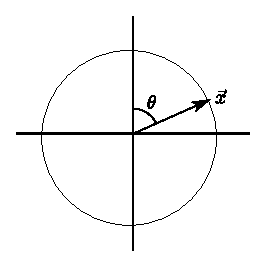
\includegraphics{05clockwise-circle-problem.pdf}
\end{center}
\endanswer




\subprob  \(x(t) =  1+\cos t \), \(y(t) = 1+\sin t  \)
\answer %{{{3
Circle with radius 1 and center $(1,1)$ (it touches the $x$ and $y$ axes).
Traversed infinitely often in counterclockwise fashion.
\begin{center}
  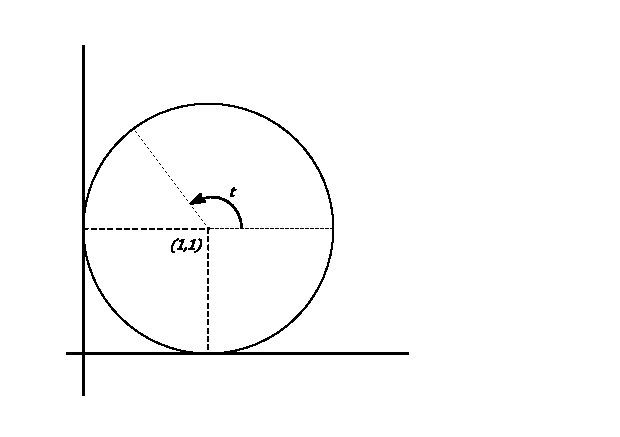
\includegraphics{05circle-at-1-1-problem.pdf}
\end{center}
\endanswer




\subprob  \(x(t) =  2\cos t \), \(y(t) = \sin t  \)
\answer %{{{3
Without the $2$ this would be the standard unit circle (dashed curve below).
Multiplying the $x$ component by $2$ stretches this circle to an ellipse.  So
$(x(t), y(t))$ traces out an ellipse, infinitely often, counterclockwise.




\begin{center}
  \includegraphics{05ellipse-problem.pdf}
\end{center}




\endanswer




\subprob  \(x(t) =  t^2 \), \(y(t) = t^3  \)
\answer %{{{3
For each $y=t^3$ there is exactly one $t$, namely, $t=y^{1/3}$.  So the curve is
a graph (with $x$ as a function of $y$ instead of the other way around).  It
is the graph of $x=y^{2/3} = \sqrt[3]{y^2}$.
\begin{center}
  \input ../figures/221/05neils-problem.tex
\end{center}
The curve is called \emph{Neil's parabola}.
\endanswer




\problem Complete the steps that led to \eqref{eq:05curvature-computation}. %{{{3




\problem Find the radius of curvature and the center of the osculating circle to %{{{3
the curve $x(t)=t, y(t) = 1/t$ at the point with $t=1$.




\problem  Find the curvature of the graph of a function $y=f(x)$.  You %{{{3
can do this be thinking of the graph of $y=f(x)$ as a parametric
curve as in \S~\ref{sec:motion-on-a-graph}, and then using
\eqref{eq:05curvature-of-parametrized-curve}.




The result you should get is
\[
\kappa = \frac{f''(x)} {\bigl(1+f'(x)^2\bigr)^{3/2}}\;.
\]




\problem Use the result from the previous problem to find points with the %{{{3
largest or smallest curvature on the following familiar graphs.  In each case
make a drawing of the graph first and guess your answer before you compute it.




\subprob Where is the curvature of the graph of $y=x^2$ largest?




\subprob Where is the curvature of the graph of $y=x^3$ largest?




\subprob Where is the curvature of the graph of $y=\frac13x^3$ largest?




\problem \carefulnow  Compute the curvature of the parametric curve given by %{{{3
$x(t) = \cos^2 t$, $y(t) = \sin^2 t$.




The answer turns out to be very simple and could have been predicted without
taking any derivatives -- do you see why?
\answer %{{{3
Since $\sin^2t + \cos^2 t =1$ we have $y(t) = 1-x(t)$ on this curve.  The curve
is a straight line and therefore its curvature is zero.
\endanswer




% \problem Consider the parametric curve %{{{3
% \[
%   x(t)=\frac{1-t^2}{1+t^2}, \quad y(t)=\frac{2t}{1+t^2}.
% \]
% \subprob Show that the curve traces out part of the unit circle.




% \subprob For which value of $t$ is $(x,y)=(1,0)$?  \; $(0,1)$?  $(0,-1)$? \;
% $\left(\frac35,\frac45\right)$?\;
% $\left(\frac{\sqrt{2}}{2},\frac{\sqrt{2}}{2}\right)$?\; Is there a value of $t$
% for which $(x,y)=(-1,0)$?












\end{multicols}
\noproblemfont




\section{l'Hopital's rule} %{{{1
\label{sec:05lhopitals-rule}




There is a simple way to compute limits of the form
\[
\lim_{t\to a} \frac{f(t)} {g(t)}
\]
that are of the form $\frac{0} {0}$, i.e.~where
\[
\lim_{t\to a} f(t) = 0
\text{ and }
\lim_{t\to a} g(t) = 0.
\]
It is given by what is called l'Hopital's rule, which says the
following:




\begin{theorem}
  If $f$ and $g$ both are differentiable functions such that 
  \[
    \lim_{t\to a} f(t) = 0 \text{ and } \lim_{t\to a} g(t) = 0,
  \]
  and if
  $\displaystyle \lim_{t\to a} \frac{f'(t)} {g'(t)}$ exists, then $\lim_{t\to a}
  \frac{f(t)} {g(t)} $ also exists.  Moreover,
  \[
    \lim_{t\to a} \frac{f(t)} {g(t)} = \lim_{t\to a} \frac{f'(t)} {g'(t)}
  \]
\end{theorem}\smallskip




\subsection{The reason why l'Hopital's rule works} %{{{2
\label{sec:reason-for-lHopital}
The two functions $f$ and $g$ define a parametric curve $x=g(t)$, $y=f(t)$
that is defined for $t\geq a$.  At $t=0$ we have $x=g(a) = 0$ and $y=g(a) = 0$,
so the origin lies on the curve traced out by $x=g(t)$, $y=f(t)$.




\noindent\rule{\textwidth}{1pt}\medskip




\def\mvtforlHopitalAnnotation
 {{\begin{minipage}{2.8in}\sffamily\itshape\footnotesize The slope of the chord
        connecting the origin and the point $(g(t), f(t))$ is
        \[\dfrac{f(t)}{g(t)}.\]

        Somewhere between this point and the origin there is a point $(g(c),
        f(c))$ on the curve where the tangent has the same slope. The slope of
        the tangent is
        \[\dfrac{f'(c)}{g'(c)}\]
      \end{minipage}
}}
\noindent%
\input ../figures/221/05mvt-for-lHopital2.pdf_tex%




\noindent\rule{\textwidth}{1pt}\smallskip

If we pick any value of $t>a$, then the ratio $\frac{f(t)} {g(t)}$ is the slope
of the chord connecting the two points $(0,0)$ and $(g(t), f(t))$ on the curve.
By the same kind of reasoning that led to the Mean Value Theorem (see Figure
\ref{fig:05MeanValueTheorem}) there has to be a point in between where the
tangent to the curve is parallel to the chord: in other words, there is some $c$
with $a<c<t$ such that
\[
\frac{f(t)} {g(t)} = \frac{f'(c)} {g'(c)}.
\]
The number $c$ depends on $t$, but since it lies between $a$ and $t$, we have
$\lim_{t\to a}c = a$.  
Therefore
\[
\lim_{t\to a}\frac{f(t)} {g(t)} = \lim_{c\to a}\frac{f'(c(t))} {g'(c(t))} =
\frac{f'(a)} {g'(a)}.
\]








 
\subsection{Examples of how to use l'Hopital's rule} %{{{2
The limit
\[
\lim_{x\to 1} \frac{3x^2-x-2} {x^2-1}
\]
is of the form $\frac{0} {0}$, so we can try to apply l'Hopital's rule.  We
get
\begin{equation}
\lim_{x\to 1} \frac{3x^2-x-2} {x^2-1}
=
\lim_{x\to 1} \frac{6x-1} {2x}
\label{eq:05lHopital-example1}
\end{equation}
So far we don't know if the limit exists, so it could be that we are
just saying that two things that don't exist are equal (whatever that
means).  But the second limit does exits:
\[
\lim_{x\to 1} \frac{6x-1} {2x} = \frac{6-1} {2} = \frac{5} {2}.
\]
Since this exists, l'Hopital's rule tells us that
the first limit in \eqref{eq:05lHopital-example1} also exists, and is
equal to $\frac52$.




For another example, consider the limit
\[
\lim_{x\to 0} \frac{\sin x} {x}
\]
which we have already computed in Chapter~III, \S\ref{sec:trigLimit}.  It is again
a limit of the form $\frac00$, so we can try to use l'Hopital's rule:
\[
\lim_{x\to 0} \frac{\sin x} {x} = \lim_{x\to0} \frac{\cos x} {1}
\stackrel{(*)}= \frac{1} {1} =1.
\]
The reasoning is that since the limit of $\dfrac{\cos x} {1}$ exists,
the limit of $\dfrac{\sin x}x$ must also exist and be the same.


Note that evaluating the limit $\lim_{x\to 0} \frac{\sin x} {x} = 1$ in this manner is actually circular reasoning, because we used this same limit in showing that the derivative of $\sin(x)$ is $\cos(x)$.


In the same way you can do a slightly more complicated example
\[
\lim_{x\to 0} \frac{\sin 5x} {\tan x}
=\text{``}\tfrac00\text{''}
\stackrel{\text{l'H}}=
\lim_{x\to0} \frac{5\cos 5x} {1/\cos^2x}
\stackrel{{(*)}}= \frac{5\cdot 1} {1/1^2} = 5.
\]
Again, the equality ``$\stackrel{\text{l'H}}=$''  follows from
l'Hopital's rule and the next equality ``$\stackrel{(*)}=$'' justifies
using the rule.




\subsection{Examples of repeated use of l'Hopital's rule} %{{{2
The limit
\[
\lim_{x\to 0} \frac {x - \sin x}{x^3}
\]
is again of the form $\frac00$.  When you apply l'Hopital's rule you
get
\[
\lim_{x\to 0} \frac {x - \sin x}{x^3}
=
\lim_{x\to 0} \frac {1 - \cos x}{3x^2},
\]
which is also of the form $\frac00$!  That means we can try to compute
this new limit by again applying l'Hopital's rule.  Here is the whole
computation:
\[
  \lim_{x\to 0} \frac {x - \sin x}{x^3}
  = \lim_{x\to 0} \frac {1 - \cos x}{3x^2}
  = \lim_{x\to 0} \frac {\sin x}{6x}
  = \lim_{x\to 0} \frac {\cos x}{6}
  = \tfrac16.
\]
Here we have applied l'Hopital's rule three times.  When we do this we
don't know if any of the limits that we run into actually exist, until
at the very end we find that the last limit exists (it's $\frac16$ in
this example).  The fact that the last limit exists implies that the
one before that exists; the fact the second to last limit exists in
turn implies that the limit before that one exists, and so on, until
we conclude that the limit we started with exists.  All the limits
must be equal, so we find that
\[
  \lim_{x\to 0} \frac {x - \sin x}{x^3} = \frac16,
\]
which means that for small values of $x$ we have the approximation
\[
x-\sin x \approx \tfrac16 x^3.
\]








\section{Problems} %{{{1
\problemfont %{{{3
\begin{multicols}{2}
\problem Compute the following limits using l'Hopital's rule. %{{{3




\subprob $\displaystyle \lim_{x\to 0} \frac{x^2-3} {x^2-8x-9}$.




\subprob $\displaystyle\lim_{x\to \pi/2} \frac{\sin 2x} {\cos x}$.




\subprob $\displaystyle\lim_{x\to 1/2} \frac{\cos \pi x} {1-2x}$.








\problem Suppose $n$ is some positive integer, and the limit %{{{3
\[
\lim_{x\to0} \frac{\cos x -1 -x^2/2} {x^n} = L
\]
exists. Also suppose $L\neq0$.
What is $n$?  What is the limit $L$?












\problem What happens when you use l'Hopital's rule to compute these %{{{3
limits?




\subprob $\displaystyle\lim_{x\to 0} \frac{x^2} {x}$.




\subprob $\displaystyle\lim_{x\to 0} \frac{x^2} {x^3}$.




\problem  Let $f(x) = \frac12x + x^2\sin\frac\pi x$ be the strange %{{{3
function whose graph is drawn in Figure
\ref{fig:05zigzagBetweenParabolas}.




\subprob Try to compute
\[
\lim_{x\to 0} \frac{f(x)} {x}
\]
in two ways:
\begin{itemize}
\item directly, and
\item by using l'Hopital's rule.
\end{itemize}




\subprob \carefulnow\carefulnow~~The following rule sounds very much
like l'Hopital's:
\begin{center}
  \itshape if $\displaystyle\lim_{x\to a} \frac{f(x)} {g(x)}$ exists,
  then $\displaystyle\lim_{x\to a} \frac{f'(x)} {g'(x)}$ also exists,
  and the two limits are equal.
\end{center}
But this is not always true!  Find a counterexample.








\problem Here is a method for computing derivatives: since, by %{{{3
definition,
\[
f'(a) = \lim_{x\to a} \frac{f(x) - f(a)} {x-a}
\]
is a limit of the form $\frac00$, we can always try to find it by
using l'Hopital's rule.  What happens when you do that?




\problem Simplicio did the following computation %{{{3
\begin{align*}
  \lim_{x\to 0} \frac{x} {\sin x}
  &= \lim_{x\to 0} \frac{1} {\cos x}\\
  &= \lim_{x\to 0} \frac{0}{\sin x}\\
  &= \lim_{x\to 0} 0\\
  &= 0\ldots?
\end{align*}
Do you see any problems with this?




\end{multicols}
\noproblemfont

%%% Local Variables:
%%% mode: latex
%%% TeX-master: "free221"
%%% End:

% !TEX root =  free221.tex
\chapter{Exponentials and Logarithms (naturally)}
\label{ch:exponentials}
% !!! Issue: Limits of sequences are assumed here, but are not defined anywhere
In this chapter we first recall some facts about exponentials ($x^y$ with $x>0$
and $y$ arbitrary): they should be familiar from algebra, or ``precalculus''.
What is new is perhaps the definition of $x^y$ when $y$ is not a rational
number: for example, we know that $2^{3/4}$ is the 4th root of the third power
of 2 ($\sqrt[4]{2^3}$), but what should we take as the definition of something
like $2^{\sqrt{2}}$?

Next we ask ``what is the derivative of $f(x)=a^x$?'' The answer leads us to the
famous number $e\approx 2.718\, 281\, 828\, 459\, 045\, 235\, 360\, 287\, 471\,
352\, 662\, 497\, 757\, 247\, 093\, 699\, 95\cdots$.

Finally, we compute the derivative of $f(x)=\log_a x$, and we discuss the notion
of ``exponential growth''.


\section{Exponents} %{{{1
Here we discuss the definition of $x^y$ when $x$ and $y$ are arbitrary
real numbers, with $x>0$.




For any real number $x$ and any positive integer $n=1, 2, 3, \ldots$ one defines
\[
x^n = \overbrace{x\cdot x\cdot \cdots \cdot x}^{\text{$n$ times}}
\]
and, if $x\neq0$,
\[
x^{-n} = \frac1{x^n}.
\]
One defines $x^0=1$ for any $x\ne0$.




To define $x^{p/q}$ for a general fraction $\frac p q$ one must assume
that the number $x$ is positive. One then defines
\begin{equation}\label{eq:pqpowerofx-def}
  x^{p/q}= \sqrt[q]{x^p}.
\end{equation}
This does not tell us how to define $x^a$ is the exponent $a$ is not a fraction.
One can define $x^a$ for irrational numbers $a$ by taking limits.  For example,
to define $2^{\sqrt{2}}$, we look at the sequence of numbers obtained by truncating
the decimal expansion of $\sqrt{2}$, namely
\[
a_1 = 1,
\qquad   a_2= 1.4=\tfrac{14}{10},
\qquad    a_3=1.41=\tfrac{141}{100},
\qquad a_4= 1.414=\tfrac{1414}{1000},
\qquad   \cdots.
\]
Each $a_n$ is a rational number, so we know what $2^{a_n}$ is; for example,
$2^{a_4} = \sqrt[1000]{2^{1414}}$.  Our definition of $2^{\sqrt{2}}$ then is
\[
2^{\sqrt{ 2}} = \lim_{n\to\infty} 2^{a_n},
\]
which is to say, we define $2^{\sqrt{2}}$ as the ``limit of the sequence''
\[
2, \sqrt[10]{2^{14}}, \sqrt[100]{2^{141}}, \sqrt[1000]{2^{1414}}, \cdots
\]
(See table \ref{tbl:07twototheroottwo}.)




\begin{table}[htp]
  \begin{center}
    \begin{tabular}{ll}
      \toprule
      $x=\dfrac pq$  &  $\displaystyle 2^x = \sqrt[q]{2^p}$\\
      \midrule
      1.0000000000=$\frac11$ &
      \textbf{2}\textit{\textcolor{red}{.000000000000}}  \\[2pt]
      1.4000000000=$\frac{14}{10}$ &
      \textbf{2.6}\textit{\textcolor{red}{39015821546}}  \\[2pt]
      1.4100000000=$\frac{141}{100}$  &
      \textbf{2.6}\textit{\textcolor{red}{57371628193}}  \\[2pt]
      1.4140000000 &  \textbf{2.66}\textit{\textcolor{red}{4749650184}}  \\
      1.4142000000 &  \textbf{2.6651}\textit{\textcolor{red}{19088532}}  \\
      1.4142100000 &  \textbf{2.6651}\textit{\textcolor{red}{37561794}}  \\
      1.4142130000 &  \textbf{2.66514}\textit{\textcolor{red}{3103798}}  \\
      1.4142135000 &  \textbf{2.665144}\textit{\textcolor{red}{027466}}  \\
      $\vdots$  &\hspace{24pt} $\vdots$\\
      \bottomrule
    \end{tabular}
  \end{center}\smallskip
  \caption{Approximating $2^{\sqrt{2}}$ by computing $2^x$ for rational
numbers $x$.  Note that as $x$ gets closer to $\sqrt2$ the quantity
$2^x$ appears to converge to some number.  This limit is our
definition of $2^{\sqrt{2}}$.}
  \label{tbl:07twototheroottwo}
\end{table}%








Here one ought to prove that this limit exists, and that its value does not
depend on the particular choice of numbers $a_n$ tending to $a$. We will not go
into these details in this course.




In precalculus you learn that the exponential functions satisfy the
following properties:
\begin{equation}\label{eq:exponential-properties}
  x^a x^b = x^{a+b}, \qquad
  \dfrac{x^a}{x^b} = x^{a-b}, \qquad
  \bigl(x^a\bigr)^b = x^{ab}
\end{equation}
provided $a$ and $b$ are rational numbers. In fact these properties still
hold if $a$ and $b$ are arbitrary real numbers. Again, we
won't go through the proofs here.




Now instead of considering $x^a$ as a function of $x$ we can pick a positive
number $a$ and consider the function $f(x) = a^x$. This function is defined for
all real numbers $x$ (as long as the base $a$ is positive.).




\subsection{The trouble with powers of negative numbers. } %{{{2
The cube root of a negative number is well defined.  For instance,
$\sqrt[3]{-8}=-2$ because $(-2)^3 = -8$.  In view of the definition
\eqref{eq:pqpowerofx-def} of $x^{p/q}$ we can write this as
\[
(-8)^{1/3} = \sqrt[3]{(-8)^1} = \sqrt[3]{-8} = -2.
\]
But there is a problem: since $\frac{2}{6}=\frac13$ we might think that
$(-8)^{2/6} = (-8)^{1/3}$.  However our definition \eqref{eq:pqpowerofx-def}
tells us that
\[
(-8)^{2/6} = \sqrt[6]{(-8)^2} = \sqrt[6]{+64} =  +2.
\]
Another example:
\[
(-4)^{1/2} = \sqrt{-4} \text{ is not defined}
\]
but, even though $\frac12=\frac24$,
\[
(-4)^{2/4} = \sqrt[4]{(-4)^2}  = \sqrt[4]{+16} = 2 \text{ is defined.}
\]

There are two ways out of this mess: either
\begin{enumerate}\sffamily\itshape
\item avoid taking fractional powers of negative numbers, or
\item whenever we compute $x^{p/q}$, we first simplify the fraction by removing
  common divisors of $p$ and $q$.
\end{enumerate}
The safest option is just not to take fractional powers of negative numbers.




Given that fractional powers of negative numbers cause all these
headaches it is not surprising that we didn't try to define $x^a$ for
negative $x$ if $a$ is irrational.  For example, $(-8)^\pi$ is not
defined\footnote{There is a definition of $(-8)^\pi$ which uses complex
numbers, but we won't see or need this in the calculus sequence; it
will show up in math 319 or 320 where complex exponentials are
treated, and you will also run into $(-8)^\pi$ if you take an
electrical engineering course where ``phasors'' are discussed}.



\section{Logarithms} %{{{1
Briefly, if $a$ is a positive constant not equal to 1, then we define $y=\log_a
x$ to be the inverse function to $y=a^x$. This means that, by definition,
\[
y=\log_a x \iff x=a^y.
\]
In other words, $\log_a x$ is the answer to the question ``for which number $y$
does one have $x=a^y$?''  The number $\log_a x$ is called \emph{the logarithm of
$x$ to the base $a$}.  Note that since exponentials are always positive, the
logarithm of 0 or of a negative number is not defined\footnote{Again, there is a
way to define logarithms of negative numbers using complex numbers. We will not
pursue these ideas at the moment.}


For instance,
\[
2^3 = 8, \quad
2^{1/2} = \sqrt2,\quad
2^{-1}= \frac12
\]
so
\[
\log_2 8 = 3,\quad
\log_2\bigl(\sqrt{2}\bigr) = \frac12,\quad
\log_2 \frac12 = -1.
\]
Also:
\[
\log_2 (-3) \text{ doesn't exist}
\]
because there is no number $y$ for which $2^y = -3$ ($2^y$ is always positive)
and
\[
\log_{-3}2 \text{ doesn't exist either}
\]
because $y=\log_{-3}2$ would have to be some real number which satisfies $(-3)^y
= 2$, and we don't take non-integer powers of negative numbers.






\section{Properties of logarithms} %{{{1
In general one has
\[
\log_a a^x = x,  \text{ and }  a^{\log_a x}=x.
\]
There is a subtle difference between these formulas: the first one holds for all
real numbers $x$, but the second only holds for $x>0$, since $\log _a x$ doesn't
make sense for $x\leq 0$.




Again, you learn the following formulas in precalculus:
\begin{equation}
  \begin{aligned}
    \log_a xy &= \log_a x + \log _a y \\
    \log_a \frac xy &= \log_ax-\log_a y
  \end{aligned}
  \qquad\qquad
  \begin{aligned}
    \log_a x^y &= y\log_a x \\
    \log_a x &= \dfrac{\log_b x}{\log_b a}
  \end{aligned}
  \label{eq:07logarithm-properties}
\end{equation}
They follow from \eqref{eq:exponential-properties}, and to review this
subject it is good to write out the reason why $a^{p+q} = a^p a^q$
implies $\log_a xy = \log_a x + \log_a y$, and similarly for the other
formulas in \eqref{eq:07logarithm-properties}.




\section{Graphs of exponential functions and logarithms} %{{{1
Figure \ref{fig:07expplot} shows the graphs of some exponential
functions $y=a^x$ with different values of $a$, and Figure
\ref{fig:07logplot} shows the graphs of $y=\log_2 x$, $y=\log_3 x$,
$\log_{1/2}x$, $\log_{1/3}(x)$ and $y=\log_{10}x$.




\begin{figure}[t]\centering
  
    \begin{picture} (270.000000,140.322581)(0,0)
    \put(0.0, 0.0){\includegraphics{07expplot.pdf}}
        \put(  3.32,  -6.68){\sffamily\itshape -3}
    \put( 46.55,  -6.68){\sffamily\itshape -2}
    \put( 89.77,  -6.68){\sffamily\itshape -1}
    \put(133.00,  -6.68){\sffamily\itshape  0}
    \put(176.23,  -6.68){\sffamily\itshape  1}
    \put(219.45,  -6.68){\sffamily\itshape  2}
    \put(262.68,  -6.68){\sffamily\itshape  3}
    \put(138.00,  88.77){\sffamily\itshape 2}
    \put(138.00, 132.00){\sffamily\itshape 3}
\end{picture}

  \caption{The graphs of $y=2^x, 3^x, (1/2)^x, (1/3)^x$ and $y=(4/5)^x$.
    The graphs are purposely not labeled: can you figure out which is which?}
  \label{fig:07expplot}
\end{figure}




From precalculus we recall:
\begin{itemize}
\item If $a>1$ then $f(x)=a^x$ is an increasing function of $x$.
\item If $0<a<1$ then $f(x)=a^x$ is a decreasing function of $x$.
\end{itemize}
In other words, for $a>1$ it follows from $x_1<x_2$ that
$a^{x_1}<a^{x_2}$; if $0<a<1$, then $x_1<x_2$ implies $a^{x_1} >
a^{x_2}$.

These statements can be shown using the properties \ref{eq:exponential-properties}.  However, we might also try to show these properties by computing the derivatives of these functions.


\section{The derivative of $a^x$ and the definition of $e$} %{{{1
To begin, we try to differentiate the function $y=2^x$:
\begin{align*}
  \frac{d}{dx}\left[ 2^x \right]
  & = \lim_{\Delta x\to0}\frac{2^{x+\Delta x}-2^x}{\Delta x} \\
  & = \lim_{\Delta x\to0}\frac{2^{x}2^{\Delta x}-2^x}{\Delta x} \\
  & = \lim_{\Delta x\to0}2^x\frac{2^{\Delta x}-1}{\Delta x} \\
  & = 2^x \lim_{\Delta x\to0}\frac{2^{\Delta x}-1}{\Delta x}.
\end{align*}




So if we assume that the limit
\[
\lim_{\Delta x\to0}\frac{2^{\Delta x}-1}{\Delta x}=C
\]
exists, then we have
\begin{equation}
  \label{eq:derivativeof2x}
  \frac{d 2^x}{dx} = C 2^x.
\end{equation}
On your calculator you can compute $\frac{2^{\Delta x}-1}{\Delta x}$
for smaller and smaller values of $\Delta x$, which leads you to
suspect that the limit actually does exist, and that $C\approx
0.693\;147\;\ldots$. One can in fact prove that the limit exists, but
we will not do this here.




\begin{figure}[!t]\centering
  
    \begin{picture} (360.000000,214.673267)(0,0)
    \put(0.0, 0.0){\includegraphics{07logplot.pdf}}
        \put( 37.99,  95.34){\sffamily\itshape  1}
    \put( 73.44,  95.34){\sffamily\itshape  2}
    \put(108.88,  95.34){\sffamily\itshape  3}
    \put(144.33,  95.34){\sffamily\itshape  4}
    \put(179.77,  95.34){\sffamily\itshape  5}
    \put(215.22,  95.34){\sffamily\itshape  6}
    \put(250.66,  95.34){\sffamily\itshape  7}
    \put(286.11,  95.34){\sffamily\itshape  8}
    \put(321.55,  95.34){\sffamily\itshape  9}
    \put(357.00,  95.34){\sffamily\itshape 10}
    \put( -5.46,  -2.00){\sffamily\itshape -3}
    \put( -5.46,  33.45){\sffamily\itshape -2}
    \put( -5.46,  68.89){\sffamily\itshape -1}
    \put( -5.46, 104.34){\sffamily\itshape 0}
    \put( -5.46, 139.78){\sffamily\itshape 1}
    \put( -5.46, 175.23){\sffamily\itshape 2}
    \put( -5.46, 210.67){\sffamily\itshape 3}
\end{picture}

  \caption{Graphs of some logarithms.  Each curve is the graph of a
    function $y=\log_a x$ for various values of $a>0$.  Can you tell
    what $a$ is for each graph?}
  \label{fig:07logplot}
\end{figure}








Once we know \eqref{eq:derivativeof2x} we can compute the derivative of $a^x$
for any other positive number $a$. To do this we write $a=2^{\log_2 a}$,
and hence
\[
a^x = \bigl( 2^{\log_2 a} \bigr)^x = 2^{x\cdot \log_2 a}.
\]
By the Chain Rule we therefore get
\begin{align*}
  \frac{da^x}{dx} &= \frac{d}{dx}\left[2^{x\cdot \log_2 a}\right] \\
  &= C\;2^{x\cdot \log_2 a}\; \frac{d}{dx}\left[x\cdot \log_2 a\right] \\
  &=C\;2^{x\cdot \log_2 a}\cdot \log_2 a \\
  &= (C\log_2 a) \;a^x.
\end{align*}
So the derivative of $a^x$ is just some constant times $a^x$, the constant being
$C\log_2a$.  This is essentially our formula for the derivative of $a^x$, but
one can make the formula look nicer by introducing a special number
\[
e=2^{1/C}\text{ where  }
C=\lim_{ \Delta x\to0} \frac{2^{ \Delta x} - 1}{ \Delta x}.
\]
One has
\[
e\approx 2.718\;281\;828\;459\;045\;\cdots
\]
The definition ``$e = 2^{1/C}$'' looks completely random and
unmotivated, but here is the reason why $e=2^{1/C}$ is a special
number: if you set $a=e$, then
\[
C\log_2 a = C\log_2 e = C\log_2 2^{1/C} = C\cdot \frac1C =1,
\]
and therefore the derivative of the function $y=e^x$ is
\begin{equation}
  \label{eq:derivative-of-ex}
  \frac{de^x}{dx} = e^x.
\end{equation}
Read that again: the function $e^x$ is its own derivative!




The logarithm with base $e$ is called the \emph{Natural Logarithm},
and is written
\[
\ln x = \log_e x.
\]
Thus we have
\begin{equation}
  e^{\ln x}  = x \qquad  \ln e^x = x
\end{equation}
where the second formula holds for all real numbers $x$ but the first one
only makes sense for $x>0$.




For any positive number $a$ we have $a=e^{\ln a}$, and also
\[
a^x = e^{x\ln a}.
\]
By the Chain Rule you then get
\begin{equation}
  \label{eq:derivative-of-ax}
  \dfrac{da^x}{dx} = a^x\ln a.
\end{equation}




\section{Derivatives of Logarithms} %{{{1
Since the logarithm $f(x)=\log_a x$ is the inverse function of the exponential
$g(x) = a^x$, we can find its derivative by implicit differentiation: we know
that
\[
a^{f(x)} = x.
\]
Differentiating both sides, and using the Chain Rule on the left gives
\[
(\ln a)  a^{f(x)} f'(x) = 1.
\]
Now solve for $f'(x)$ to get
\[
f'(x) = \frac{1}{(\ln a) a^{f(x)}}.
\]
Finally we remember that $a^{f(x)} = x$, and this gives us the derivative of $a^x$:
\[
\frac{da^x}{dx} = \frac{1}{x\ln a}.
\]
In particular, the natural logarithm has a very simple derivative: since $\ln
e=1$, we have
\begin{equation}\label{eq:derivative-of-ln}
 \frac{d}{dx}\left[\ln x\right] = \frac{1}{x}.
\end{equation}


\section{Limits involving exponentials and logarithms} %{{{1
\begin{theorem}  Let $r$ be any real number.  Then, if $a>1$,
  \[
  \lim_{x\to\infty} x^r a^{-x} = 0,
  \]
  i.e.
  \[
  \lim_{x \to\infty}\frac{x^r}{a^x} = 0.
  \]
\end{theorem}
This theorem says that \textit{any exponential will beat any power of $x$ as
  $x\to\infty$}.  For instance, as $x \to\infty$ both $x^{1000}$ and $(1.001)^x$
go to infinity, but
\[
\lim_{x \to\infty} \frac{x^{1000}}{(1.001)^x} = 0,
\]
so, in the long run, for very large $x$, $1.001^x$ will be much larger than
$1000^x$.


% !!! Discuss: Instead we could just repeatedly use L'Hopital's rule at
% infinity. That proof is much less horrible.

% l'Hopital's rule was not proved for f/g where f, g\to\infty.
% The rule also encourages not thinking about "how large function are"
% Its use should be discouraged.  This section should be modified to include the
% list of functions in their natural magnitude
%               (log << powers of x << exponential functions)
%

\begin{proof}[Proof when $a=e$]
  We want to show $\lim_{x\to\infty} x^re^{-x} = 0$.  To do this consider the
  function $f(x) = x^{r+1}e^{-x}$.  Its derivative is
  \[
  f'(x) = \frac{dx^{r+1}e^{-x}}{dx}
  = \bigl((r+1)x^r - x^{r+1}\bigr)e^{-x}
  = (r+1-x)x^re^{-x}.
  \]
  Therefore $f'(x) < 0$ for $x>r+1$, i.e.\ $f(x)$ is decreasing for $x>r+1$.
  It follows that $f(x) <f(r+1)$ for all $x>r+1$, i.e.
  \[
  x^{r+1}e^{-x} < (r+1)^{r+1}e^{-(r+1)}\text{ for } x>r+1.
  \]
  Divide by $x$, abbreviate $A=(r+1)^{r+1}e^{-(r+1)}$, and we get
  \[
  0<x^re^{-x}<\frac Ax \text{ for all }x>r+1.
  \]
  The Sandwich Theorem implies that $\lim_{x\to\infty} x^re^{-x} = 0$, which
  is what we had promised to show.

The case with general $a$ follows after a substitution:  given $a$ we set 
\[
 x=\frac{t}{\ln a}. 
\]
Then, since $a>1$ we have $\ln a>0$ so that as $x\to\infty$ one also has $t\to\infty$.  Therefore
\[
 \lim_{x\to\infty}
 \frac{x^r}{a^x}
 = 
 \lim_{x\to\infty}
 \frac{x^r}{e^{x\ln a}}
 = 
 \lim_{t\to\infty}
 \frac{(t/\ln a)^r}{e^{t}}
 = \underbrace{(\ln a)^{-r}}_{\textsf{constant}}\cdot 
 \underbrace{\lim_{t\to\infty}
 \frac{t^r}{e^{t}}}_{=0}
 =0.
\]


\end{proof}




\subsection{Related limits} %{{{2
If $a$, $m$, and $r$ are constants, then
\begin{subequations}
  \begin{align}
    a>1 \implies &
    \lim_{x \to\infty} \frac{a^x}{x^r} = \infty \quad(D.N.E.)
    \label{eq:07exp-beats-power-limit}\\
    m>0 \implies & \lim_{x \to\infty} \frac{\ln x}{x^m} =0
        \label{eq:07power-beats-log-atinfty-limit}\\
    m>0 \implies & \lim_{x \to 0} x^m\ln x =0
        \label{eq:07power-beats-log-atzero-limit}
  \end{align}
\end{subequations}
The second limit (\ref{eq:07power-beats-log-atinfty-limit}) says that even
though $\ln x$ becomes infinitely large as $x \to\infty$, it is always much less
than any power $x^m$ with $m>0$ real.  To prove it you set $x=e^t$ and then
$t=s/m$, which leads to
\[
\lim_{x \to\infty} \frac{\ln x}{x^m}
\;\stackrel{x=e^t}{=}\;
\lim_{t \to\infty} \frac{t}{e^{mt}}
\;\stackrel{t = s/m}{=}\;
\frac1m\;\lim_{t \to\infty}\frac{s}{e^s} = 0.
\]
The limit (\ref{eq:07power-beats-log-atzero-limit}) follows from the second by
substituting $x=1/y$ and using $\ln\frac1x = -\ln x$.




\section{Exponential growth and decay} %{{{1
\subsection{Absolute and relative growth rates} %{{{2
If a quantity $X(t)$ changes with time, then the change in $X$ during a short
time interval of length $\Delta t$ is
\[
\Delta X = X(t+\Delta t) - X(t).
\]
If $X$ is measured in certain units, then the change $\Delta X$ has
the same units as $X$.  The change $\Delta X$ is sometimes called the
\emph{absolute change}, to distinguish it from the \emph{relative
  change,} which is defined as
\[
\text{Relative change in $X$ }= \frac{\Delta X} {X}.
\]
No matter what units $X$ is measured in, the relative change has no
units and can be expressed as a percentage.  For instance, if the
population $X$ of a city increases from $200,000$ to $250,000$
(people), then the absolute population change is $50,000$ (people),
but the relative population change is
\[
\frac{50,000\text{ people}}
{200,000\text{ people}} =
\frac{1} {4} = 25\%.
\]
Just as we defined the rate of change of a quantity $X(t)$ to be
\[
\frac{dX} {dt} = \lim_{\Delta t\to0} \frac{\Delta X} {\Delta t},
\]
we define the \emph{relative rate of change} or \emph{relative growth
  rate} to be
\[
\lim_{\Delta t \to 0}
\frac{\left\{
    \parbox{90pt}{\sffamily\centering%
      Relative change in $X$\\
      from $t$ to $t+\Delta t$ }
  \right\}} {\Delta t}
= \lim_{\Delta t \to 0} \frac{\Delta X} {X \Delta t}
= \frac{1} {X}\frac{dX} {dt}.
\]




\subsection{Theorem on constant relative growth} %{{{2
\label{sec:07const-relative-growth}
\itshape%
Suppose that a time-dependent quantity $X(t)$ has a constant relative
growth rate, meaning that
\begin{equation}
  \frac{1} {X} \frac{dX} {dt} = k \text{ is constant.}
  \label{eq:07constant-relative-growth}
\end{equation}
And suppose that at time $t_0$ the value of $X$ is known to be
$X(t_0) = X_0$.  Then
\begin{equation}\label{eq:07exponentialgrowth}
  X(t) = X_0 e^{k(t-t_0)}.
\end{equation}
\upshape



% !!! Issue: The proof assumes the result that a function with zero derivative is constant! This does not appear in the text anywhere.
\begin{proof}
  The constant relative growth rate condition
  \eqref{eq:07constant-relative-growth} implies
  \begin{equation}\label{eq:07exp-growth-diffeq}
    \frac{dX(t)}{dt} = kX(t).
  \end{equation}
  The trick is to look at the rate of change of $e^{-kt}X(t)$:
  \begin{align*}
    \frac{dX(t)e^{-kt}}{dt}
    &=X(t)\frac{de^{-kt}}{dt} + \frac{dX(t)}{dt}e^{-kt}\\
    &=-kX(t) e^{-kt}+X'(t)e^{-kt}\\
    &= (X'(t) - kX(t))e^{-kt} \\
    &=0.
  \end{align*}
  In other words $X(t)e^{-kt}$ does not depend on $t$.  Therefore
  \[
  X(t)e^{-kt} = X(t_0) e^{-kt_0} = X_0 e^{-kt_0}, \text{ for any $t$.}
  \]
  Multiply with $e^{kt}$ and we end up with
  \[
  X(t) = X_0e^{k(t-t_0)}.
  \]
\end{proof}
The equations \eqref{eq:07constant-relative-growth} and
\eqref{eq:07exp-growth-diffeq} are examples of \textit{differential
  equations}.  They are equations in which the unknown quantity $X$ is
not a number but a function, and in which the derivative of the
unknown function appears.  We have just reasoned that any function
that satisfies \eqref{eq:07constant-relative-growth} (has constant
relative growth) must be of the form \eqref{eq:07exponentialgrowth}:
we have solved the differential equation\footnote{The trick we used here is an
example of solving differential equations by multiplying with an ``integrating
factor''.  We will do this more systematically in Math 222.}.




\subsection{Examples of constant relative growth or decay} %{{{2
\label{sec:07examples-of-const-relative-growth}
Here is a typical scenario of constant relative growth or, rather,
decay.  Suppose that the molecules of a certain chemical substance
appear in two varieties, the ``normal'' kind A, and the ``excited''
kind A$^*$.  Left to themselves the normal kind of molecules A are
stable, but the excited kind will randomly decay to the normal kind.
In the long run all A$^*$ will be converted into regular A molecules.
One example of this kind of reaction is radioactive decay where, say,
\raisebox{-3pt}{\footnotesize14}C decays to
\raisebox{-3pt}{\footnotesize14}N.  There are \textit{many} other
similar examples.




{\itshape%
  How fast does the conversion from {\upshape A}$^*$ to {\upshape A}
  happen?}  A very common reasoning to find the conversion rate goes
like this.  Suppose $X(t)$ is the total amount of A$^*$ and suppose
that during a short time interval of length $\Delta t$ a certain
number of conversions from A$^*$ to A take place.  If the time
interval is short, then the number of conversions will be small, and
the total amount $X(t)$ of A$^*$ molecules will not change much.
Therefore, during the next short time interval of length $\Delta t$
you would expect the same number of conversions to happen.  Adding
these together you conclude that if you wait twice as long ($2\Delta
t$) then the number of conversions doubles; more generally, you would
expect the number of conversions during a short time interval of
duration $\Delta t$ to be proportional to $\Delta t$.




If on the other hand you fix the length of the time interval, but
double the amount of A$^*$ molecules, you would expect twice as many
conversions to occur, so, the number of conversions from A$^*$ to A
during some short time interval $\Delta t$ should also be proportional
with the amount of A$^*$ present.
\marginpar{\sffamily\footnotesize%
  To say that a reaction takes place in which A$^*$ decays
  to A you could write:\\
\centerline{A$^* \stackrel{k}\longrightarrow$ A.}\\
The $k$ above the arrow is the ``reaction rate.''  }


Putting this together, we see that the change in the amount of A$^*$
during a time interval of length $\Delta t$ should be proportional
both with $X$ and with $\Delta t$, so
\[
\Delta X \approx - k\cdot X\cdot \Delta t,
\]
for some constant $k$.  The approximation should be better as you make
the time interval shorter, and therefore, dividing by $X\Delta t$ and
taking the limit $\Delta t\to0$, we see that the amount of $X$ should
satisfy
\[
\frac{1} {X} \frac{dX} {dt} = -k,
\]
which is \eqref{eq:07constant-relative-growth}, but with $k$ replaced
by $-k$.  The conclusion is: if you know that at time $t_0$ the
amount of A$^*$ is $X(t_0) = X_0$, then at any other time $t$,
\[
X(t) = X_0 e^{-k(t-t_0)}.
\]








\subsection{Half time and doubling time. } %{{{2
If $X(t) = X_0 e^{kt}$ then one has
\[
X(t+T) = X_0e^{kt+kT} = X_0e^{kt}e^{kT} = e^{kT}X(t).
\]
In words, after a time $T$ goes by, an exponentially growing (decaying) quantity
changes by a factor $e^{kT}$.  If $k>0$, so that the quantity is actually
growing, then one calls
\[
T = \frac{\ln 2}{k}
\]
the \emph{doubling time} for $X$ because $X(t)$ changes by a factor $e^{kT} =
e^{\ln2} = 2$ every $T$ time units:  $X(t)$ doubles every $T$ time units.




If $k<0$ then $X(t)$ is decaying and one calls
\[
T = \frac{\ln 2}{-k}
\]
the \emph{half life} because $X(t)$ is reduced by a factor $e^{kT} = e^{-\ln 2}
= \frac12$ every $T$ time units.




\subsection{Determining $X_0$ and $k$. } %{{{2
The general exponential growth/decay function \eqref {eq:07exponentialgrowth}
contains only two constants, $X_0$ and $k$, and if you know the values of $X(t)$
at two different times then you can compute these constants.

Suppose that you know
\[
X_1 = X(t_1) \text{ and } X_2=X(t_2).
\]
Then we have
\[
X_0e^{kt_1} = X_1 \text{ and } X_2 = X_0e^{kt_2}
\]
in which $t_1, t_2, X_1, X_2$ are given and $k$ and $X_0$ are unknown.  
One first finds $k$ from
\[
\frac{X_1}{X_2}= \frac{X_0e^{kt_1}}{X_0e^{kt_2}}
=e^{k(t_1-t_2)}
\implies \ln\frac{X_1}{X_2}= k(t_1-t_2)
\]
which implies
\[
k = \frac{\ln X_1 - \ln X_2}{t_1-t_2}.
\]
Once you have computed $k$ you can find $X_0$ from
\[
X_0 = \frac{X_1}{e^{kt_1}} = \frac{X_2}{e^{kt_2}}.
\]
(both expressions should give the same result.)
















\section{Problems} %{{{1
\problemfont %{{{3




\begin{multicols}{2}
\noindent\textbf{Sketch the graphs} of the following functions.
You should
\begin{list}{--}{
    \setlength{\itemindent}{0pt}
    \setlength{\leftmargin}{6pt}}
\item find where $f$, $f'$ and $f''$ are positive or negative
\item find all stationary points and classify them as local minima, maxima, or neither
\item find any global maxima or minima, if they exist
\item find all inflection points
\item determine all intervals where the function is increasing or decreasing
\item determine all intervals where the function is convex or concave
\item find any horizontal, vertical, or slant asymptotes
\end{list}



(\textit{Hint for some of these:  if you have to solve something like
  $e^{4x}-3e^{3x}+e^x = 0$, then call $w=e^x$ to get a polynomial
  equation $w^4-3w^3+w=0$ for $w$.})




\problem $\DS y= e^x $ %{{{3




\problem $\DS y= e^{-x} $ %{{{3




\problem $\DS y= e^{x}+e^{-2x} $ %{{{3
\answer %{{{3
$dy/dx = e^x - 2e^{-2x}$. Local min at $x = \frac13 \ln 2$.




$d^2y/dx^2 = e^x+4e^{-2x}>0$ always, so the function is convex.




$\lim_{x\to\pm\infty} y=\infty$, no asymptotes.
\endanswer




\problem $\DS y= e^{3x}-4e^x $ %{{{3
\answer %{{{3
$dy/dx = 3e^{3x} - 4 e^x$. Local min at $x=\frac12\ln\frac43$.




$d^2y/dx^2 = 9e^{3x} - 4e^{x}$ changes sign when $e^{2x} = \frac49$,
i.e.~at $x=\frac12\ln\frac49 = \ln\frac23 = \ln2-\ln3$.  Inflection
point at $x=\ln2-\ln 3$.




$\lim_{x\to-\infty}f(x) = 0$ so negative $x$ axis is a horizontal
asymptote.




$\lim_{x\to\infty}f(x) = \infty$\ldots no asymptote there.
\endanswer




\problem $\DS y= \frac{e^x}{1+e^x} $ %{{{3




\problem $\DS y= \frac{2e^x}{1+e^{2x}} $ %{{{3




\problem $\DS y= xe^{-x} $ %{{{3




\problem $\DS y= \sqrt{x}e^{-x/4} $ %{{{3




\problem $\DS y= x^2 e^{x+2} $ %{{{3




\problem $\DS y= e^{x/2}-x$ %{{{3




\problem $\DS y= \ln \sqrt x $ %{{{3




\problem $\DS y= \ln \frac1 x $ %{{{3




\problem $\DS y= x\ln x $ %{{{3




\problem $\DS y= \frac{-1}{\ln x}  \quad(0<x<\infty, x\neq1)$ %{{{3




\problem $\DS y= (\ln x)^2  \quad(x>0)$ %{{{3




\problem $\DS y= \frac{\ln x}{x} \quad(x>0)$ %{{{3




\problem $\DS y=\ln \sqrt{\frac{1+x}{1-x}} \quad(|x|<1)$ %{{{3




\problem $\DS y= \ln \bigl(1+x^2\bigr) $ %{{{3




\problem $\DS y= \ln \bigl(x^2-3x+2\bigr) \quad (x>2) $ %{{{3




\problem $\DS y= \ln\cos x\quad (|x|< \tfrac{\pi}{2})$ %{{{3




\problem $\DS y = \sqrt{e^{2x}}$ %{{{3




\problem The function $f(x) = e^{-x^2}$ plays a central role in %{{{3
statistics and its graph is called \emph{the bell curve} (because of its
shape).  Sketch the graph of $f$.




\problem Sketch the part of the graph of the function %{{{3
\[
f(x) = e^{-\frac1x}
\]
with $x>0$.
Find the limits
\[
\lim_{x\searrow 0} \frac{f(x)}{x^n}
\text{ and }
\lim_{x \to\infty} f(x)
\]
where $n$ can be any positive integer. (Hint: substitute $y=1/x$.)

\problem A \emph{damped oscillation} is a function of the form %{{{3
\[
f(x) = e^{-ax} [\cos b(x-c)]
\]
where $a$, $b$, and $c$ are constants.

\subprob $g(x) = e^{-x} \sin 10x$ is a damped oscillation.  What are
the constants $a$, $b$, and $c$?

\subprob Draw the graphs of $y=e^{-x}$, $y=-e^{-x}$, and $y=g(x)$
in one sketch (with pencil and paper).  Make sure you include the
piece of the graph with $0\leq x\leq 2\pi$.

\subprob $y=g(x)$ has many local maxima and minima.  
\textit{What is the ratio between the function values at two consecutive
  local maxima?}  (Hint: the answer does not depend on which pair of
consecutive local maxima you consider.)


\problem Find the inflection points on the graph of $f(x) = (1+x)\ln x$, for $x>0$. %{{{3



\problem \textbf{(a)~}If $x$ is large, which is bigger: $2^x$ or $x^2$?\\ %{{{3
\textbf{(b)~}The graphs of $f(x) = x^2$ and $g(x) = 2^x$ intersect at $x=2$
(since $2^2=2^2$).  How many more intersections do these graphs have (with
$-\infty < x < \infty$)?




\bigskip
\textbf{Find the following limits.}
\begin{multicols}{2}
\problem  $\DS\lim_{x\to\infty}\frac{e^x-1}{e^x+1} $ %{{{3




\problem  $\DS\lim_{x \to\infty}\frac{e^x-x^2}{e^x+x} $ %{{{3




\problem  $\DS\lim_{x\to\infty}\frac{2^x}{3^x-2^x} $ %{{{3




\problem  $\DS\lim_{x \to\infty}\frac{e^x-x^2}{e^{2x}+e^{-x}} $ %{{{3




\problem  $\DS\lim_{x \to\infty}\frac{e^{-x}-e^{-x/2}}{\sqrt{e^x+1}} $ %{{{3




\problem  $\DS\lim_{x \to\infty}\frac{\sqrt{x+e^{4x}}}{e^{2x}+x} $ %{{{3




\problem  $\DS\lim_{x \to\infty}\frac{e^{\sqrt x}}{\sqrt{e^x}} $ %{{{3




\problem  $\DS\lim_{x \to \infty} \frac{e^{\sqrt{x}}} {\sqrt{e^x+1}}$ %{{{3




\problem  $\DS\lim_{x \to\infty}\frac{\ln x}{\ln (x^2)} $ %{{{3




\problem  $\DS\lim_{x \to 0} x\ln x$ %{{{3




\problem  $\DS\lim_{x\to\infty}\frac{\ln x}{\sqrt x+\ln x} $ %{{{3




\problem  $\DS\lim_{x\to 0}\frac{\ln x}{\sqrt x+\ln x} $ %{{{3




\end{multicols}
\problem  $\DS\lim_{x \to\infty}\ln (1+x) - \ln x$ %{{{3








\problem  Find the tenth derivative of $xe^x$.  Then find the $99$th %{{{3
derivative of $xe^{x}$.




\problem For which real number $x$ is $2^x- 3^x$ the largest? %{{{3








\problem Find $\DS\frac{dx^x}{dx} $, $\DS\frac{d x^{x^x}}{dx}$, and %{{{3
$\DS\frac{d(x^x)^x}{dx} $.




\null\hfill Hint: write $x^x$ as $e^{\text{something}}$.







% !!! Issue: The other problems on logarithmic differentiation should be moved here and combined, into an actual explanation of the technique.
\problem \groupproblem \textit{About logarithmic differentiation -- %{{{3
see Problem \ref{ex:05log-derivs}.}




\subprob  Let $y=(x+1)^2(x+3)^4(x+5)^6$ and $u=\ln y$.  Find $du/dx$. Hint:
Use the fact that $\ln$ converts multiplication to addition before you
differentiate.  It will simplify the calculation.




\subprob  Check that the derivative of $\ln u(x)$ is the logarithmic
derivative of the function $u$.












\problem After $3$ days a sample of radon-222 decayed to $58\%$ of its original %{{{3
amount.

\subprob What is the half-life of radon-222?

\subprob How long would it take the sample to decay to $10\%$ of its
original amount?

\problem   Polonium-210 has a half-life of $140$ days. %{{{3

\subprob If a sample has a mass of $200$mg, find a formula for the
mass that remains after $t$ days.

\subprob Find the mass after 100 days.

\subprob When will the mass be reduced to 10 mg?

\subprob Sketch the graph of the mass as a function of time.








% \problem %{{{3
% Current agricultural experts believe that the world's farms can feed about
% 10 billion people.  The 1950 world population was 2.517 billion and the 1992
% world population was 5.4 billion.  When can we expect to run out of food?








% \problem \groupproblem The AC\textit{ME} company runs two ads on %{{{3
% Sunday mornings. One says
% that ``when this baby is old enough to vote, the world will have one
% billion new mouths to feed'' and the other says ``in thirty six years,
% the world will have to set eight billion places at the table.''  What
% does AC\textit{ME} think the population of the world is at present?
% How fast does AC\textit{ME} think the population is increasing?  Use
% units of billions of people so you  can write $8$ instead of
% $8,000,000,000$.  (Hint: $36=2\times 18$.)








% \problem The population of California grows exponentially at an instantaneous %{{{3
% rate of 2\% per year.  The population of California on January 1,
% 2000 was 20,000,000.




% \subprob Write a formula for the population $N(t)$ of California
% $t$ years after January 1, 2000.




% \subprob Each Californian consumes pizzas at the rate of 70
% pizzas per year.  At what rate is California consuming pizzas $t$
% years after 1990?




% \subprob How many pizzas were consumed in California from January
% 1, 2005 to January 1, 2009?

\problem Here are three versions of the same problem (read all \& choose one): %{{{3

\subprob The number of individuals of an endangered species decreases to half
its size every $1000$ days.  How long does it take for the population to
decrease to $75\%$ of its current size?

\subprob A radioactive substance has a half-life of $1000$ years.  How long does
it take for $25\%$ of it to decay?

\subprob The concentration of gas released in a chamber has a half-life of
$1000$ seconds. How long it would take for the gas to lower its concentration to
$75\%$ of its initial level?

\problem The remains of an old campfire are unearthed and it is found that there %{{{3
is only $80\%$ as much radioactive carbon-14 in the charcoal samples from the
campfire as there is in modern living trees.  If the half-life of carbon-14 is
$5730$ years, how long ago did the campfire burn?


\problem Max needs 1 gram of Kryptonite to perform an important experiment. %{{{3
Unfortunately, he doesn't have the lab set up for his experiment yet and his
Kryptonite is decaying.  Yesterday there were 15 grams of Kryptonite left and
today there are only 12 grams left.  How long does he have before he won't
have enough Kryptonite left to do his experiment?

\problem Two equivalent problems -- read them and pick one: %{{{3
% This problem requires a(n easy) substitution to solve, which is probably too hard.



\subprob ({\it Newton's law of cooling})
Newton's law of cooling states that the rate of change of temperature $T$
of an object is proportional to the difference between its temperature
and the ambient temperature, $U$, that is,
\[
  \frac{dT}{dt}=k\left(U-T(t)\right).
\]




A body is discovered at $7$ am. Its temperature is then $25^{\circ}$ C. By the
time police arrives at the site, at $8$ pm, the body has cooled at $20^{\circ}$
C. Assuming the normal body temperature in humans is $37^{\circ}$ C, and that
the ambient temperature is $5^{\circ}$ C, determine the time of death.




\subprob A nuclear reactor was shut down for maintenance repairs. The rate of
change of temperature in the fuel rods of the reactor is described by Newton's
law of cooling:
\[
  \frac{dT}{dt}=k\left(U-T(t)\right),
\]
where $U=5^{\circ}$ C is the temperature of the water being pumped into the
reactor. The normal temperature of the fuel rods in a working reactor is
$37^{\circ}$ C.  If at $7$ am, the temperature of fuel rods was $25^{\circ}$ C,
and an hour later the fuel rods have cooled at $20^{\circ}$ C, when was the
reactor shut down?




\problem A bacteria population grows exponentially with growth rate $k=2.5$. How %{{{3
long it will take for the bacteria population to double its size?




\problem Three equivalent problems -- read all and do one: %{{{3




\subprob The half-life of a certain drug in the human body is $8$ hours. How
long it would take for a dose of this drug to decay to $0.1\%$ of its initial
level?




\subprob After a nuclear plant explosion, radioactive material is scattered in
the atmosphere. Particularly dangerous for human health is the iodine-131,
whose half-life is $8$ days. How long it would take for the iodine-131 in the
atmosphere to decay to $0.1\%$ of its initial level?




\subprob The concentration of gas released in a chamber has a half-life of $8$
minutes. How long it would take for the gas to lower its concentration to
$0.1\%$ of its initial level?




\problem The \textit{hyperbolic functions} are defined by %{{{3
\begin{gather*}
  \sinh x = \frac{e^x-e^{-x}}2,\\
  \cosh x = \frac{e^x+e^{-x}}2,\\
  \tanh x = \frac{\sinh x}{\cosh x}.
\end{gather*}
\subprob Prove the following identities:
\begin{gather*}
  \cosh^2 x -\sinh^2 x = 1\\
  \cosh 2x = \cosh^2x + \sinh ^2 x \\
  \sinh 2x = 2\sinh x \cosh x.
\end{gather*}
\subprob Show that
\begin{gather*}
  \frac{d\sinh x}{dx} = \cosh x, \\
  \frac{d\cosh x}{dx} = \sinh x, \\
  \frac{d\tanh x}{dx} = \frac1{\cosh^2 x}.
\end{gather*}
\subprob Sketch the graphs of the three hyperbolic functions.








\problem Sketch the following parametrized curves %{{{3
(first review Chapter~V, \S\ref{sec:05parametrized-curves-and-lHopital}):




\subprob \(x(t) =  e^t \), \(y(t) = e^t  \)
\answer %{{{3
The diagonal $y=x$ again, but since $x=e^t$ can only be positive we only get the
part in the first quadrant.  At $t=-\infty$ we start at the origin, as
$t\to+\infty$ both $x$ and $y$ go to $+\infty$.
\endanswer




\subprob \(x(t) =  e^t \), \(y(t) = t  \)
\answer %{{{3
The graph of $y=\ln x$, or $x=e^y$ (same thing), traversed in the upwards
direction.
\endanswer




\subprob \(x(t) =  e^t \), \(y(t) = e^{-t}  \)
\answer %{{{3
The part of the graph of $y=1/x$ which is in the first quadrant, traversed from
left to right.
\endanswer




\problem \subprob At which point on the graph of $y=e^x$ is the %{{{3
curvature the largest?




\subprob At which point on the graph of $y=\ln x$ is the
curvature the largest?

\end{multicols}
\noproblemfont


%%% Local Variables:
%%% mode: latex
%%% TeX-master: "free221"
%%% End:

% !TEX root =  free221.tex
\chapter{The Integral}
In this chapter we define the integral of a function on an interval $[a,b]$,
introduce the Fundamental Theorem of Calculus relating integration and
differentiation, and develop basic techniques for computing integrals.

The most common interpretation of the integral is in terms of the area under the
graph of the given function, so that is where we begin.


\section{Area under a Graph} %{{{1
Let $f$ be a function which is defined on an interval $a\leq x\leq
b$ and assume it is positive (so that its graph lies above
the $x$ axis). \textit{How large is the area of the region caught
  between the $x$ axis, the graph of $y=f(x)$ and the vertical lines
  $y=a$ and $y=b$?}
\begin{figure}[h]
    \parbox{0.45\textwidth}{
    \begin{picture} (150.000000,70.307692)(0,0)
    \put(0.0, 0.0){\includegraphics{08AreaUnderGraph.pdf}}
        \put( 16.08,  -5.31){\sffamily\itshape $a$}
    \put(129.92,  -5.31){\sffamily\itshape $b$}
    \put( 78.00,  38.15){\sffamily\itshape $y=f(x)$}
\end{picture}
}
    \parbox{0.45\textwidth}{
    \begin{picture} (150.000000,70.307692)(0,0)
    \put(0.0, 0.0){\includegraphics{08Riemann-fine.pdf}}
        \put( 17.08,  -7.31){\sffamily\itshape $a$}
    \put(129.92,  -7.31){\sffamily\itshape $b$}
\end{picture}
}
\end{figure}
We can try to compute this area (on the left here) by approximating
the region with many thin rectangles (on the right).  The idea is that
even though we don't know how to compute the area of a region bounded
by arbitrary curves, we do know how to find the area of one or more
rectangles.

To write formulas for the area of those rectangles we first have to
introduce some notation -- have a look at Figure~\ref{fig:08Riemann}
before reading on.  To make the approximating region, we choose a
\emph{partition} of the interval $[a, b]$: we pick numbers
$x_1<\cdots<x_n$ with
\[
a=x_0 < x_1 < x_2 < \cdots < x_{n-1}< x_n = b.
\]
These numbers split the interval $[a, b]$ into $n$ sub-intervals
\[
[x_0, x_1], \quad [x_1, x_2],\quad \ldots,\quad [x_{n-1}, x_n]
\]
whose lengths are
\[
\Delta x_1 = x_1-x_0, \quad \Delta x_2 = x_2 - x_1, \quad\ldots, \quad
\Delta x_n = x_n-x_{n-1}.
\]
In each interval $[x_{k-1},x_k]$, we choose a \emph{sample point} $c_k$: thus in
the first interval we choose some number $c_1$ such that $x_0\leq c_1\leq x_1$,
in the second interval we choose some $c_2$ with $x_1\leq c_2\leq x_2$, and so
forth. (See Figure~\ref{fig:08Riemann}.)

We then define $n$ rectangles: the base of the $k^{\textrm{th}}$ rectangle is
the interval $[x_{k-1}, x_k]$ on the $x$-axis, while its height is $f(c_k)$
(here $k$ can be any integer from 1 to $n$).

The area of the $k^{\textrm{th}}$ rectangle is the product of its
height and width, which is $f(c_k)\Delta x_k$.  Adding up all the rectangles'
areas yields
\begin{equation}\label{eq:09riemann-sum}
  R = f(c_1)\Delta x_1 + f(c_2) \Delta x_2 + \cdots + f(c_n)\Delta x_n.
\end{equation}
This kind of sum is called a \emph{Riemann sum.}
\begin{figure}[t]
  \centering
  
    \begin{picture} (300.000000,185.384615)(0,0)
    \put(0.0, 0.0){\includegraphics{08Riemann.pdf}}
        \put( 35.38,   0.46){\sffamily\itshape \makebox[0pt][r]{$a=x_0$}}
    \put( 52.45, -11.54){\sffamily\itshape \makebox[0pt][c]{$c_1$}}
    \put( 69.77,   0.46){\sffamily\itshape \makebox[0pt][c]{$x_1$}}
    \put( 84.82, -11.54){\sffamily\itshape \makebox[0pt][c]{$c_2$}}
    \put(115.62,   0.46){\sffamily\itshape \makebox[0pt][c]{$x_2$}}
    \put(141.32, -11.54){\sffamily\itshape \makebox[0pt][c]{$c_3$}}
    \put(150.00,   0.46){\sffamily\itshape \makebox[0pt][c]{$x_3$}}
    \put(162.98, -11.54){\sffamily\itshape \makebox[0pt][c]{$c_4$}}
    \put(178.65,   0.46){\sffamily\itshape \makebox[0pt][c]{$x_4$}}
    \put(205.20, -11.54){\sffamily\itshape \makebox[0pt][c]{$c_5$}}
    \put(218.77,   0.46){\sffamily\itshape \makebox[0pt][c]{$x_5$}}
    \put(239.65, -11.54){\sffamily\itshape \makebox[0pt][c]{$c_6$}}
    \put(264.62,   0.46){\sffamily\itshape \makebox[0pt][l]{$b=x_6$}}
\end{picture}

  \bigskip
  
  \caption{\textbf{A partition, and a Riemann sum. } Here, the interval
    $a<x<b$ is divided up into six smaller intervals.  In each of
    those intervals a sample point $c_i$ is chosen, and the
    resulting rectangles with heights $f(c_1)$, \ldots\,, $f(c_6)$ are
    drawn.  The total area under the graph of the function is roughly
    equal to the total area of the rectangles.  }
  \label{fig:08Riemann}
\end{figure}

If the rectangles are all sufficiently narrow then we would expect that the total
area of all rectangles should be a good approximation of the area of the region
under the graph.  So we would expect the ``area under the curve'' to be the
limit of Riemann sums like $R$ ``as the partition becomes finer and finer''. A
precise formulation of the definition goes like this:

\begin{definition}
  If $f$ is a function defined on an interval $[a, b]$, then we say
  that
  \[
  \int_a^b f(x) dx = I,
  \]
  read as ``the integral of $f(x)$ from $x=a$ to $b$ equals $I$'', if
  for every $\varepsilon >0$, one can find a $\delta>0$ such that
  \[
  \Bigl|f(c_1)\Delta x_1 + f(c_2) \Delta x_2 + \cdots + f(c_n)\Delta
  x_n -I\Bigr|<\varepsilon
  \]
  holds for every partition all of whose intervals have length $\Delta
  x_k<\delta$ with any arbitrary choice of sample points $c_1$, \dots , $c_n$. 
\end{definition}

This is a perfectly good definition, but it's not even clear that the limit
exists even for comparatively simple functions like $f(x)=x$, let alone for more
complicated functions.  It turns out that, with a fair amount of effort, one can
prove that this limit always exists provided that $f(x)$ is a continuous
function on the interval $[a,b]$.  Even so, it is quite hard to evaluate areas
this way.

\section{When $f$ changes its sign} %{{{1
If the function $f$ is not necessarily positive everywhere in the interval
$a\leq x\leq b$, then we still define the integral in exactly the same way: as a
limit of Riemann sums whose mesh size becomes smaller and smaller.  However the
interpretation of the integral as ``the area of the region between the graph and
the $x$-axis'' has a twist to it.

\begin{figure}[h]
  \centering

  
    \begin{picture} (240.000000,137.081081)(0,0)
    \put(0.0, 0.0){\includegraphics{08Riemann-posandneg.pdf}}
        \put( 19.30,  53.32){\sffamily\itshape $a$}
    \put(211.27,  69.32){\sffamily\itshape $b$}
\end{picture}


  \caption{\textbf{Riemann sum for a function whose sign
    changes.}  Always remember this:\\
    \centerline{\bfseries  INTEGRALS CAN BE NEGATIVE, BUT}
    \centerline{\bfseries AREAS ARE ALWAYS POSITIVE NUMBERS.}\\[2pt]
    The Riemann-sum corresponding to this picture is the total area of
    the rectangles above the $x$-axis \textit{minus} the total area of
    the rectangles below the $x$-axis. }

  \label{fig:08Riemann-posandneg}
\end{figure}

Let $f$ be a function on the interval $a\leq x\leq b$, and form the
Riemann sum
\[
R = f(c_1)\Delta x_1 + f(c_2) \Delta x_2 + \cdots + f(c_n)\Delta x_n
\]
that goes with some partition, and some choice of $c_k$.

When $f$ can be positive or negative, then the terms in the Riemann
sum can also be positive or negative.  If $f(c_k)>0$ then the quantity
$f(c_k)\Delta x_k$ is the area of the corresponding rectangle, but if
$f(c_k)<0$ then $f(c_k)\Delta x_k$ is a negative number, namely
$-1$ times the area of the corresponding rectangle.  The Riemann
sum is therefore the area of the rectangles above the $x$-axis
\textit{minus} the area of the rectangles below the $x$-axis.  Taking
the limit over finer and finer partitions, we conclude that
\[
\int_a^b f(x) dx =
\begin{array}[c]{c}
  \text{area above the $x$-axis, below the graph of $y=f(x)$} \\
  \text{\emph{minus}}\\
  \text{the area below the $x$-axis, above the graph of $y=f(x)$} 
\end{array}
\]

\section{The Fundamental Theorem of Calculus} %{{{1
% !!! Issue: Only half of the fundamental theorem is actually here! The other
% half, about differentiating an integral, is completely missing.
% !!! Issue: There is no discussion whatsoever of the proof of the FToC nor even
% a discussion of why it's intuitively true.
% 
% Sigurd: This should eventually be included.  For now the instructor must present a
% proof in lecture.  The best would be to create an animation that explains the
% whole circle of ideas.
%
\begin{definition}
  A function $F$ is called an \emph{antiderivative} of $f$ on the
  interval $[a, b]$ if one has $F'(x) = f(x)$ for all $x$ with
  $a\leq x \leq b$.
\end{definition}
\smallskip

For instance, $F(x) = \frac12 x^2$ is an antiderivative of $f(x) = x$,
but so are $G(x) = \frac12 x^2+1$ and $H(x) = \frac12x^2 + 2012$.
%  !!! Issue: Needed theorem: Continuous functions have antiderivatives!

\begin{theorem}
  If $f$ is a function whose integral $\int_a^b f(x) dx$ exists, and if
  $F$ is an antiderivative of $f$ on the interval $[a,b]$, then one has
  \begin{equation}
    \label{eq:fundamental-theorem}
    \int_a^b f(x) dx = F(b) - F(a).
  \end{equation}
\end{theorem}
(a proof was given in lecture.)

Because of this theorem the expression on the right appears so often
that various abbreviations have been invented.  We will abbreviate
\[
F(b)-F(a) \stackrel{\text{def}}{=} \bigl. F(x)\bigr]_{x=a}^b =
\bigl.F(x)\bigr]_a^b .
\]

\subsection{Terminology}\label{sec:08terminology} %{{{2
In the integral
\[
\int_a^b f(x)\;dx
\]
the numbers $a$ and $b$ are called the \textit{limits of integration}, the
function $f(x)$ which is being integrated is called \textit{the integrand}, and
the variable $x$ is \textit{integration variable.}

The integration variable is a \textit{dummy variable}.  If we
systematically replace it with another variable, the resulting
integral will still be the same. For instance,
\[
\int_0^1 x^2\,dx = \bigl.\tfrac13 x^3\bigr|_{x=0}^1 = \tfrac13,
\]
and if we replace $x$ by $\varphi$ we still get
\[
\int_0^1 \varphi^2\, d\varphi
= \bigl.\tfrac13 \varphi^3\bigr|_{\varphi=0}^1 = \tfrac13.
\]
Another way to appreciate that the integration variable is a dummy
variable is to look at the Fundamental Theorem again:
\[
\int_a^b f(x)\;dx = F(b) -F(a).
\]
The right hand side tells you that the value of the integral depends
on $a$ and $b$, and has absolutely nothing to do with the variable $x$.

\section{Summation notation} %{{{1
\label{sec:09about-those-dots}
A Riemann sum is a summation with very many terms: more to the point, a Riemann
sum usually has ``$n$ terms'' where $n$ is allowed to vary.  For such a sum we
cannot write all terms in the way we can for a sum that has, say, 25 terms.
This is why our formulas for Riemann sums, such as \eqref{eq:09riemann-sum},
\[
  R = f(c_1)\Delta x_1 + f(c_2) \Delta x_2 + \cdots + f(c_n)\Delta x_n
\]
contain dots ($\cdots$) to represent the terms we didn't explicitly write.
Even though we did not write most of the terms in this sum it is clear what they
are, just from looking at the pattern of the first two and the last term.

If we don't like the ambiguity created by the dots in the Riemann sum, then we
can use summation notation: if we have a sum with $n$ terms, and if we
have a formula $a_k$ for term number $k$ in the sum, then we write
\[
  \sum_{k=1}^n a_k = a_1+a_2+\cdots+a_n.
\]
The expression on the right is pronounced as ``the sum from $k=1$ to $n$ of
$a_k$''.  For example,
\[
  \sum_{k=3}^7 k^2 = 3^2 + 4^2 + 5^2 + 6^2 + 7^2,
\]
which adds up to $9+16+25+36+49 = 135$.

With this notation we can write the Riemann sum \eqref{eq:09riemann-sum} as
\[
  R = f(c_1)\Delta x_1 + f(c_2) \Delta x_2 + \cdots + f(c_n)\Delta x_n
  = \sum_{k=1}^n f(c_k) \Delta x_k.
\]
The advantage of $\Sigma$ notation is that it takes the guesswork out of the
summation:  we don't have to guess what the 23$^{\rm rd}$ term is because there
is a formula in which we can just substitute $k=23$.  If we don't care for the
$\Sigma$ notation (like the author of this text, but perhaps unlike your
instructor) then our writing has to be so clear that the reader can easily
guess what the dots represent when we write them.

Using $\Sigma$ notation our definition of the integral is often written in
the following form
\begin{equation}
  \int_a^b f(x) dx
  =
  \lim_{n\to\infty} \sum_{k=1}^n f(c_k) \Delta x_k.
  \label{eq:09integral-def-using-sigma-notation}
\end{equation}
This way of writing the definition of the integral gives a hint of where the
integral sign came from.  On the right a $\Sigma$ (the greek upper case ``S'')
was used to denote a summation.
\marginpar{\centering\sffamily\itshape\footnotesize%
\framebox{\includegraphics{08long-s.pdf}}\\[1ex]
The ``long s'' from which the integral sign derives.
}
On the left is an integral, which is not really
a sum, but a limit of sums.  To denote it, Leibniz chose an
$S$, which in the typesetting of his time looked like a ``long~s,'' and which today
looks more like an \textit{f} than an \textit{s}.


\section{Problems} %{{{1
\problemfont %{{{3
\begin{multicols}{2}\setlength{\parindent}{0pt}
\problem  %{{{3
\subprob What is a Riemann sum of a function $y=f(x)$ on an interval $a\leq
x \leq b$?

\subprob Compute $\sum_{k=1}^4 \frac{1}{k}$.
\answer %{{{3
$\sum_{k=1}^4 \frac{1}{k}
= \frac{1}{1} +  \frac{1}{2} + \frac{1}{3} + \frac{1}{4}$.

This adds up to $\frac{25}{12}$, but the point of this question was to get the
above answer.
\endanswer

\subprob Compute $\sum_{k=4}^7 2^k$.
\answer %{{{3
$2^4 + 2^5 +2^6 + 2^7$.
\endanswer

\problem Let $f$ be the function $f(x) = 1-x^2$. %{{{3

\subprob Draw the graph of $f(x)$ with $0\le x\le2$.

\subprob Compute the Riemann-sum for the partition
\[
0<\tfrac13<1<\tfrac32<2
\]
of the interval $[a, b] = [0, 2]$ if we choose each $c_k$ to be the
left endpoint of the interval it belongs to.  Draw the corresponding
rectangles (add them to our drawing of the graph of $f$).

\subprob Compute the Riemann-sum you
get if you choose the $c_k$ to be the
right endpoint of the interval it belongs to.  Make a new drawing of
the graph of $f$ and include the rectangles corresponding to the right
endpoint Riemann-sum.
\answer %{{{3
Choosing left endpoints for the $c$'s gives you
\[
f(0)\frac13 + f(\frac13)\frac23 + f(1)\frac12 + f(\frac32)\frac12
=\cdots
\]
Choosing right endpoints gives
\[
f(\frac13)\frac13 + f(1)\frac23 + f(\frac32)\frac12 + f(2)\frac12
\]
\endanswer

\problem \itshape The analog of the Fundamental Theorem for finite sums.\upshape %{{{3
% The wording of this problem needs some work
In this problem you'll compute 
\[
  1+3+5+7+\cdots+159
\]
in a smart way.  First note that there are $80$ terms, and that the $k$th term
is $f(k) = 2k-1$, so you really are going to compute
\[
  f(1) + f(2) + \cdots + f(80).
\]
\subprob Show that for the function $F(k) = k^2$, it is true that $F(k)-F(k-1) =
f(k).$
\answer %{{{3
$F(n) - F(n-1) = n^2 - (n-1)^2 = n^2 - (n^2-2n+1) = 2n-1 = f(n)$.
\endanswer
\subprob Compute $S = f(1)+f(2)+\cdots f(80)$ in terms of the function
$F$.  
\answer %{{{3
Substitute $f(1) = F(1) - F(0)$, $f(2) = F(2) - F(1)$, etc\ldots 

You get many terms, and almost all of them cancel:
\[
\begin{array}{lrcl}
  &f(1) & = & \cancel{F(1)} - F(0) \\
  &f(2) & = & \cancel{F(2)} - \cancel{F(1)} \\
  &f(3) & = & F(3) - \cancel{F(2)} \\
   && \vdots &\\
   &f(79) & = & \cancel{F(79)} - F(78) \\
   +&f(80) & = & F(80) - \cancel{F(79)} \\[4pt]
  \hline      
  &\rule{0pt}{12pt}
  S & = & F(80) - F(0) \\
\end{array}
\]
So the answer is 
\[
  f(1)+\cdots+f(80) = F(80) - F(0).
\]
In the particular example where $f(n)= 2n-1$ you get
\begin{multline*}
  1+3+5+7+\cdots+157+159 \\
  = (80)^2 = 1600.
\end{multline*}
\endanswer

\problem \groupproblem Look at figure \ref{fig:08Riemann} (top). %{{{3
Which choice of intermediate points $c_1$, \ldots, $c_6$ leads to the
smallest Riemann sum?  Which choice would give you the largest
Riemann-sum?

(Note: in this problem you're not allowed to change the division points
$x_i$, only the points $c_i$ in between them.)
\answer %{{{3
The Riemann-sum is the total area of the rectangles, so to get the
smallest Riemann-sum you must make the rectangles as small as
possible.  You can't change their widths, but you can change their
heights by changing the $c_i$.  To get the smallest area we make the
heights as small as possible. So, for the \emph{smallest} possible
Riemann sum choose  $c_i$ to be the point in the interval $[x_i,
x_{i+1}]$ where $f(x)$ attains its minimum.

For the largest possible Riemann sum choose each $c_i$ to be the point
in $[x_i, x_{i+1}]$ where $f(x)$ is maximal.

In this example this means you should choose:  $c_1 = x_1$, $c_2$ somewhere
between $x_1$ and $x_2$ where $f$ has its maximum, $c_3=x_2$, $c_4=x_3$,
$c_5=x_4$, and $c_6 = x_5$.

\endanswer
%
\[
\clubsuit
\]
\begingroup
  \itshape Find an antiderivative $F(x)$ for each of the following
  functions $f(x)$.  Finding antiderivatives involves a fair amount of
  guess work, but with experience it gets easier to guess
  antiderivatives.
\endgroup


\problem $\displaystyle f(x) = 2x+1 $ %{{{3

\problem $\displaystyle f(x) = 1-3x $ %{{{3

\problem $\displaystyle f(x) = x^2-x+11 $ %{{{3

\problem $\displaystyle f(x) = x^4-x^2 $ %{{{3

\problem $\displaystyle f(x) = 1+x+\frac{x^2}{2}+\frac{x^3}{3}+\frac{x^4}{4} $ %{{{3

\problem $\displaystyle f(x) = \frac1x $ %{{{3

\problem $\displaystyle f(x) = e^x $ %{{{3

\problem $\displaystyle f(x) = \frac2x $ %{{{3

\problem $\displaystyle f(x) = e^{2x} $ %{{{3

\problem $\displaystyle f(x) = \frac1{2+x} $ %{{{3

\problem $\displaystyle f(x) = \frac{e^x-e^{-x}}2 $ %{{{3

\problem $\displaystyle f(x) = \frac1{1+x^2} $ %{{{3

\problem $\displaystyle f(x) = \frac{e^x+e^{-x}}2 $ %{{{3

\problem $\displaystyle f(x) = \frac1{\sqrt{1-x^2}} $ %{{{3

\problem $\displaystyle f(x) = \sin x $ %{{{3

\problem $\displaystyle f(x) = \frac2{1-x} $ %{{{3

\problem $\displaystyle f(x) = \cos x $ %{{{3

\problem $\displaystyle f(x) = \cos2x $ %{{{3

\problem $\displaystyle f(x) = \sin(x-\pi/3) $ %{{{3

\problem $\displaystyle f(x) = \sin x + \sin 2x $ %{{{3

\problem $\displaystyle f(x) = 2x(1+x^2)^5$ %{{{3
\[
\heartsuit
\]
\begingroup
  \itshape In each of the following exercises, draw the indicated region and
  compute its area.
\endgroup

\problem The region between the vertical lines $x=0$ and $x=1$, and between the %{{{3
$x$-axis and the graph of $y=x^3$.

\problem The region between the vertical lines $x=0$ and $x=1$, and between the %{{{3
$x$-axis and the graph of $y=x^n$ (here $n>0$, draw for $n=\frac12, 1,
2, 3, 4$).

\problem The region above the graph of $y=\sqrt x$, below the line $y=2$, and %{{{3
between the vertical lines $x=0$, $x=4$.

\problem The bounded region above the $x$-axis and below the graph of $f(x) = x^2-x^3$. %{{{3

\problem The bounded region above the $x$-axis and below the graph of $f(x) = 4x^2-x^4$. %{{{3

\problem The region above the $x$-axis and below the graph of $f(x) = 1-x^4$. %{{{3

\problem The region above the $x$-axis, below the graph of $f(x) = \sin x$, and %{{{3
between $x=0$ and $x=\pi$.

\problem The region above the $x$-axis, below the graph of $f(x) = 1/(1+x^2)$ (a %{{{3
curve known as the \textit{witch of Maria Agnesi}), and between $x=0$ and
$x=1$.

\problem The region between the graph of $y=1/x$ and the $x$-axis, and between %{{{3
$x=a$ and $x=b$ (here $0<a<b$ are constants, e.g.\ choose $a=1$ and $b=
\sqrt2$ if you have something against either letter $a$ or $b$.)

\problem The bounded region below the $x$-axis and above the graph of %{{{3
\[
f(x) = \frac1{1+x} + \frac x2 -1.
\]

\problem Compute %{{{3
\[
\int_0^{1}\sqrt{1-x^2} dx
\]
without finding an antiderivative for $\sqrt{1-x^2}$ (you can find such
an antiderivative, but it's not easy.  This integral is the area of
some region: which region is it, and what is that area?)

\problem \groupproblem Compute these integrals without finding antiderivatives. %{{{3
\[
I = \int_0^{1/2}\sqrt{1-x^2}\,dx
\]
\[
J=\int_{-1}^1 |1-x|\,dx
\]
\[
K=\int_{-1}^1 |2-x|\,dx
\]



\end{multicols}
\noproblemfont

\section{The indefinite integral} %{{{1
\label{sec:indefinite-integral}
The fundamental theorem tells us that in order to compute the integral
of some function $f$ over an interval $[a,b]$ you should first find an
antiderivative $F$ of $f$.  In practice, much of the effort required
to find an integral goes into finding an antiderivative.  In order to
simplify the computation of the integral
\begin{equation}
  \label{eq:08definite-integral}
  \int_a^b f(x) dx = F(b)-F(a)
\end{equation}
the following notation is commonly used for the antiderivative:
\begin{equation}
  \label{eq:08indefinite-integral}
  F(x) = \int f(x) d x .
\end{equation}
For instance,
\[
\int x^2 \;dx = \tfrac13x^3+C,\quad \int \sin 5x\; dx = -\tfrac15\cos 5x+C,
\quad\textrm{etc}\ldots
\]
The integral which appears here does not have the limits of integration
$a$ and $b$.  It is called an \emph{indefinite integral}, as opposed
to the integral in \eqref{eq:08definite-integral} which is called a
\emph{definite integral}.


It is important to distinguish between the two kinds of integrals.
The main differences are listed in
Table~\ref{tbl:def-vs-indef-integrals}.

\begin{table}\sffamily
  \begin{tabular}{@{\extracolsep{2em}}cc}
    \toprule[2pt]
    \bfseries Indefinite integral & \bfseries Definite integral\\[2pt]
    \midrule \\
    $\int f(x) d x$ is a function of $x$.&
    $\int_a^bf(x)d x$ is a number. \\[1ex]
    \begin{minipage}[c]{160pt}
      By definition $\int f(x)d x$ is \textit{any function of $x$
        whose derivative is $f (x)$.}
    \end{minipage} &
    \begin{minipage}[c]{160pt}
      $\int_a^b f(x)d x$ is defined in terms of Riemann sums and can
      be interpreted as the ``area under the graph of $y=f(x)$'' when $f(x)>0$.
    \end{minipage}
    \\[1ex]
    \parbox[t]{160pt}{\vspace{1pt}

      $x$ is not a dummy variable, for example, 
      \ $\int 2xd x=x^2+C$ and $\int 2td t=t^2+C$ are
      functions of different variables, 
      so they are not equal.}&
    \parbox[t]{160pt}{\vspace{1pt}

      $x$ is a dummy variable, for example,  
      $\int_0^1 2xd x=1$, and $\int_0^1 2td t=1$, 
      so $\int_0^1 2xd x=\int_0^1 2td t$.}\\
    \bottomrule[2pt]

  \end{tabular}
  \bigskip
  
  \caption{The differences between \emph{definite} and
  \emph{indefinite} integrals}
  \label{tbl:def-vs-indef-integrals}
\end{table}

\subsection{About ``$+C$''} %{{{2
\label{sec:about-+c}
Let $f (x)$ be a function defined on the interval $[a,b]$.
If $F(x)$ is an antiderivative of $f(x)$ on this interval, then for
any constant $C$ the function $\tilde F(x)=F(x)+C$ will also be an
antiderivative of $f(x)$. So one given function $f(x)$ has many
different antiderivatives, obtained by adding different constants to
one given antiderivative.

\subsection*{Theorem} %{{{2
\itshape
If $F_1 (x)$ and $F_2 (x)$ are antiderivatives of the same function
$f(x)$ on some interval $a\leq x\leq b$, then there is a constant $C$
such that $F_1 (x)=F_2 (x)+C$.\upshape

\begin{proof}
  Consider the difference $G(x)=F_1(x)-F_2(x)$. Then $G'(x) =
  F_1'(x)-F_2'(x)=f(x)-f(x)=0$, so that $G(x)$ must be constant. Hence
  $F_1(x)-F_2(x)=C$ for some constant.
\end{proof}
% !!! Issue: It is not proven or even mentioned anywhere in the differentiation chapters that a function with zero derivative is constant!

It follows that there is some ambiguity in the notation $\int f(x)\, d
x$. Two functions $F_1(x)$ and $F_2(x)$ can both equal $\int f(x)\, d
x$ without equaling each other. When this happens, they ($F_1$ and
$F_2$) differ by a constant. This can sometimes lead to confusing
situations, e.g.\ you can check that
\begin{gather*}
  \int 2\sin x\cos x\, d x = \sin^2 x + C\\
  \int 2\sin x\cos x\, d x = -\cos^2 x + C
\end{gather*}
are both correct. (Just differentiate the two functions $\sin^2x$ and
$-\cos^2x$!) These two answers look different until you realize that
because of the trig identity $\sin^2 x+\cos^2x=1$ they really only
differ by a constant: $\sin^2x= -\cos^2x+1$, and the ``$+1$'' gets absorbed into the $+C$ term.


\begin{center}
  \fbox{\parbox{3in}{\bfseries To avoid this kind of confusion we will
      from now on never forget to include the ``arbitrary constant
      $+C$'' in our answer when we compute an antiderivative.}}
\end{center}


\subsection{You can always check the answer} %{{{2
\label{sec:you-can-always}
Suppose you want to find an antiderivative of a given function $f(x)$
and after a long and messy computation
you get an ``answer'', $F(x)$, but you're not sure if you trust that it's right. Fortunately, it is easy to check: you need only differentiate the $F(x)$ you found, and if $F'(x)$
turns out to be equal to $f(x)$, then your $F(x)$ is indeed an
antiderivative.

For example, suppose that we want to find $\int \ln x\, d x$. My
cousin Louie says it might be $F(x) = x\ln x -x$.  Let's see if he's
right:
\[
\frac{d}{dx}\bigl(x\ln x-x\bigr) = x\cdot\frac1x+1\cdot\ln x-1 = \ln
x.
\]
Who knows how Louie thought of this\footnote{He took math 222 and
  learned to integrate by parts.}, but it doesn't matter: he's right!
We now know that $\int \ln x d x=x\ln x-x+C$.

% !!! TO-DO: rewrite all the entries in this table using operator notation
\begin{table}[hb]
  \centering\sffamily
  \rule[6pt]{\textwidth}{2pt}
  \begin{tabular}{r@{\,$=$\,}lr@{$\,=\,$}lp{36pt}}
      $\displaystyle f(x)$&
    $\displaystyle \frac{dF(x)} {dx} $ &
    $\displaystyle  \int f(x)\, d x  $&
    $\displaystyle  F(x)+C $ &
    \\[3ex]
    \midrule
    $\displaystyle (n+1)x^n $&
    $\displaystyle  \frac{dx^{n+1}} {dx}$ &
    $\displaystyle \int x^{n}\, d x  $&
    $\displaystyle   \frac{x^{n+1}}{n+1}+C$ &
    $n\neq -1$\\[3ex]
    $\displaystyle \frac{1}{x} $&
    $\displaystyle  \frac{d \ln |x|}{dx} $&
    $\displaystyle \int \frac{1}{x}\, d x $&
    $\displaystyle  \ln |x| +C $&
    absolute values!!\\[3ex]
    $\displaystyle e^x $&
    $\displaystyle  \frac{de^x} {dx}$ &
    $\displaystyle \int e^x\, dx $&
    $\displaystyle  e^x +C$& \\[3ex]
    $\displaystyle -\sin x $&
    $\displaystyle  \frac{d \cos x}{dx}$&
    $\displaystyle \int \sin x\, d x  $&
    $\displaystyle   -\cos x+C$\\[3ex]
    $\displaystyle  \cos x  $&
    $\displaystyle  \frac{d  \sin x}{dx}$&
    $\displaystyle \int \cos x\, d x  $&
    $\displaystyle   \sin x+C$\\[3ex]
    $\displaystyle  \tan x  $&
    $\displaystyle  -\frac{d \ln |\cos x|}{dx}$ &
    $\displaystyle \int \tan x $&
    $\displaystyle  -\ln |\cos x|+C$ &
    absolute values!!\\[3ex]
    $\displaystyle  \frac{1}{1+x^{2}} $&
    $\displaystyle   \frac{d \arctan x}{dx}$&
    $\displaystyle \int \frac{1}{1+x^{2}}\, d x  $&
    $\displaystyle   \arctan x+C$\\[3ex]
    $\displaystyle  \frac{1}{\sqrt{1-x^{2}}} $&
    $\displaystyle  \frac{d\arcsin x}{dx} $&
    $\displaystyle \int \frac{1}{\sqrt{1-x^{2}}}\, d x  $&
    $\displaystyle   \arcsin x+C $\\[3ex]
    $\displaystyle  f(x) + g(x) $&
    $\displaystyle  \frac{d F(x) + G(x)} {dx}$&
    $\displaystyle \int \{f(x)+g(x)\} \,dx $&
    $\displaystyle   F(x)+G(x)+C $&
    See \eqref{eq:integral-additive}\\[3ex]
    $\displaystyle  cf(x) $&
    $\displaystyle  \frac{d\, cF(x)} {dx}$&
    $\displaystyle \int cf(x) \,dx $&
    $\displaystyle   cF(x)+C $&
    See \eqref{eq:integral-homogeneous}\\[3ex]
  \end{tabular}
  \smallskip
  \rule[1pt]{\textwidth}{0.3pt}

  To find derivatives and integrals involving $a^x$ instead of $e^x$ use
  $a = e^{\ln a}$,\\
  and thus $a^{x} = e^{x\ln a}$, to rewrite all exponentials as $e^{\ldots}$.
  \smallskip

  The following integral is also useful, but not as important as the
  ones above:
  \[
  \int \frac{ d x}{\cos x} = \frac12 \ln\left(\frac{1+\sin x}{1-\sin x}\right) +C
  \text{ for }\cos x\neq 0.
  \]
  \rule[1pt]{\textwidth}{2pt}
  \caption{The list of the standard integrals everyone should know}
  \label{tbl:standard-integrals}
\end{table}

Table \ref{tbl:standard-integrals} lists a number of antiderivatives which you
should know.  All of these integrals should be familiar from the
differentiation rules we have learned so far, except for the integrals of
$\tan x$ and of $\dfrac1{\cos x}$.  You can check those by differentiation
(using $\ln\frac ab=\ln a-\ln b$ simplifies things a bit).


\section{Properties of the Integral} %{{{1
Just as we had a list of properties for the limits and derivatives of
sums and products of functions, the integral has similar properties.
% except integration by parts does not appear here!

Suppose we have two functions $f(x)$ and $g(x)$ with antiderivatives
$F(x)$ and $G(x)$, respectively.  Then we know that
\[
\frac{d}{dx}\bigl(F(x) + G(x)\bigr) = F'(x) + G'(x) = f(x) + g(x).
\]
In words, $F+G$ is an antiderivative of $f+g$.  Using indefinite
integrals we can write this as
\begin{equation}
  \label{eq:sum-of-antiderivs}
  \int\bigl( f(x) + g(x) \bigr)\, dx =
  \int f(x) \, dx +\int g(x) \, dx.
\end{equation}
Similarly, $\frac{d}{dx}\bigl(cF(x)\bigr) = cF'(x) = cf(x)$ implies
that
\begin{equation}
  \label{eq:constant-times-antideriv}
  \int cf(x) \, dx = c\int f(x) \, dx
\end{equation}
if $c$ is a constant.


These properties imply analogous properties for the definite integral.
For any pair of functions on an interval $[a, b]$ one has
\begin{equation}
  \label{eq:integral-additive}
  \int_a^b\bigl[f(x) + g(x) \bigr] dx = 
  \int_a^b f(x) dx + \int_a^bg(x) dx,
\end{equation}
and for any function $f$ and constant $c$ one has
\begin{equation}
  \label{eq:integral-homogeneous}
  \int_a^b cf(x) dx = c\int_a^bf(x)dx.
\end{equation}

Definite integrals have one other property for which there is no
analog in indefinite integrals: if you split the interval of
integration into two parts, then the integral over the whole is the
sum of the integrals over the parts. The following theorem says it
more precisely.

\subsection{Theorem} %{{{2
\itshape
Given $a<b<c$, and a function on the interval $[a,b]$ then
\begin{equation}
  \label{eq:integral-domain-additive}
  \int_a^b f(x)dx + \int_b^c f(x)dx = \int_a^c f(x)dx .
\end{equation}\upshape%\smallskip


\hangindent180pt\hangafter=3%
\textit{A picture proof, assuming $f(x)>0$. } The drawing shows the
graph of a positive function on some interval $a\leq x\leq c$.  The
region below the graph consists of two pieces, namely the part with
$a\leq x\leq b$ and the part with $b\leq x\leq c$.  The total area
under the graph is the sum of the areas of the two pieces.  Since the
function is positive, the areas are given by the corresponding
integrals.  The total area is\\
\hbox to 180pt{\hspace{60pt}$\displaystyle \int_a^c f(x)dx$.}\\
and it is the sum of the areas of the two smaller regions.  This
implies \eqref{eq:integral-domain-additive}.

\noindent%
\parbox[b][0pt][b]{0.4\textwidth}{\input ../figures/221/08int-atob-plus-int-btoc.pdf_tex }

\textit{A proof using the Fundamental Theorem. } Let $F$ be an
antiderivative of $f$.  Then
\[
\int_a^b f(x)dx = F(b) - F(a) \text{ and } \int_b^c f(x)dx = F(c) -
F(b),
\]
so that
\begin{align*}
   \int_a^b f(x)dx + \int_b^c f(x)dx   &= F(b) - F(a) + F(c) - F(b) \\
  &= F(c) - F(a) \\
  &=\int_a^c f(x)dx.
\end{align*}

\subsection{When the upper integration bound is less than the lower bound} %{{{2
So far we have always assumed that $a<b$ in all indefinite integrals
$\int_a^b \ldots$.  The Fundamental Theorem suggests that when $b<a$,
we should define the integral as
\begin{equation}
  \int_a^bf(x)dx = F(b)-F(a) = -\bigl(F(a)-F(b)\bigr) = -\int_b^a f(x)dx.
\end{equation}
For instance,
\[
\int_1^0 xdx = -\int_0^1 xdx = -\tfrac12.
\]



\section{The definite integral as a function of its integration bounds} %{{{1
\subsection{A function defined by an integral} %{{{2
Consider the expression
\[
I = \int_0^x t^2\, dt.
\]
What does $I$ depend on?  To find out, we calculate the integral
\[
I = \bigl[\tfrac13t^3\bigr]_0^x 
= \tfrac13 x^3 - \tfrac13 0^3
= \tfrac13 x^3.
\]
So the integral depends on $x$.  It does not depend on $t$, since $t$
is a ``dummy variable'' (see \S\ref{sec:08terminology}, where we already
discussed this point).

In this way we can use integrals to define new functions.  For
instance, we could define
\[
I(x) = \int_0^x t^2 dt,
\]
which would be a roundabout way of defining the function $I(x) = x^3/3$.  Again,
since $t$ is a dummy variable we can replace it by any other variable we like.
Thus
\[
I(x) = \int_0^x \alpha^2\, d\alpha
\]
defines the same function (namely, $I(x) = \frac13x^3$).

This example does not really define a new function, in the sense that
we already had a much simpler way of defining the same function,
namely ``$I(x) = x^3/3$.''  An example of a \textit{new} function
defined by an integral is the so called \emph{error function} from
statistics:
\begin{equation}\label{eq:08erf-defined}
  \erf(x) \isdef
  \frac2{\sqrt\pi} \int _0 ^x e^{-t^2}\;dt,
\end{equation}
so that $\erf(x)$ is the area of the shaded region in figure \ref{fig:08erf}.
\begin{figure}[h]
  \centerline{\begin{picture} (270.000000,100.266667)(0,0)
    \put(0.0, 0.0){\includegraphics{08erf.pdf}}
        \put(180.67,  55.60){\sffamily\itshape Area $=\erf(x)$}
    \put( 72.33,  75.00){\sffamily\itshape $y=\frac2{\sqrt\pi}e^{-x^2}$}
    \put(190.83,  -2.07){\sffamily\itshape $x$}

\end{picture}
}
  \caption{Definition of the Error function.  The graph is known as
    the ``Bell curve'' or the Gaussian curve.}
  \label{fig:08erf}
\end{figure}
The integral in \eqref{eq:08erf-defined} cannot be computed in terms of the
standard functions (square and higher roots, sine, cosine, exponential and
logarithms).  Since  the integral in \eqref{eq:08erf-defined} occurs very often
in statistics (in relation with the so-called normal distribution) it has been
given its own name, ``$\erf(x)$''.

\subsection{How do you differentiate a function that is defined by an integral?} %{{{2
The answer is simple, for if $f(x) = F'(x)$ then the Fundamental Theorem says
that
\[
\int_a^x f(t) \; dt = F(x) - F(a),
\]
and therefore
\[
\frac d{dx} \int_a^x f(t) \; dt =\frac d{dx}\bigl( F(x) - F(a)\bigr) = F'(x) =
f(x),
\]\marginpar{\sffamily\footnotesize%
  Note that here we use operator notation, as in
  Chapter IV, \S~\ref{sec:04operator-notation}, and that, by definition,\\[2ex]
  \(\displaystyle
  \frac{d} {dx}\int_a^x f(t) dt =\)\\[2ex]
  \null\hfill\(\displaystyle\frac{d \int_a^x f(t) dt} {dx}
  \)}%
i.e.
\[
\frac d{dx} \int_a^x f(t) \; dt = f(x).
\]
A similar calculation gives you
\[
\frac d{dx} \int_x^b f(t) \; dt = -f(x).
\]
So what is the derivative of the error function?
It is
\begin{align*}
  \erf\, '(x) 
  &= \frac d{dx} \left[ \frac2{\sqrt\pi} \int _0 ^x e^{-t^2}\;dt\right] \\
  &= \frac2{\sqrt\pi} \frac d{dx} \left[\int _0 ^x e^{-t^2}\;dt\right] \\
  &=  \frac2{\sqrt\pi} e^{-x^2}.
\end{align*}


\section{Substitution in Integrals} %{{{1
\label{sec:method-substitution}
The Chain Rule says that
\[
\frac{d F(G(x))}{d x } = F'(G(x))\cdot G'(x),
\]
so that
\[
\int F'(G(x))\cdot G'(x) \,d x = F(G(x)) +C.
\]

We can use this result to evaluate new integrals by making substitutions.

\subsection{Example} %{{{2
Consider the function $f(x) = 2x\sin (x^2+3)$. It does not appear in
the list of standard antiderivatives we know by heart. But we do
notice\marginpar{\sffamily\footnotesize%
  With practice it gets easier to recognize what
  substitution could help you compute a specific integral, 
  but even with a lot of practice, substitution is still a matter of trial and error.} that $2x =
\frac{d}{dx} (x^2+3)$. So let's call $G(x)=x^2+3$, and $F(u) = -\cos
u$, then
\[
F(G(x)) = -\cos (x^2+3)
\]
and
\[
\frac{dF(G(x))}{dx} = \underbrace{\sin (x^2+3)}_{F'(G(x))}\cdot
\underbrace{\vphantom{(}2x}_{G'(x)} = f(x),
\]
so that
\begin{equation}
  \label{eq:substitution-example1}
  \int 2x\sin (x^2+3)\,d x = -\cos (x^2+3)+C.
\end{equation}



\subsection{Leibniz notation for substitution} %{{{2
\label{sec:leibniz-notation}
The most transparent way of computing an integral by substitution is
by following Leibniz and introduce new variables.  Thus to evaluate the
integral
\[
\int f(G(x)) G'(x)\,d x
\]
where $f(u) = F'(u)$, we introduce the substitution $u=G(x)$, and
agree to write
\[
d u = d G(x) = G'(x)\,d x.
\]
Then we get
\[
\int f(G(x)) G'(x)\,d x = \int f(u) \,d u = F(u)+C.
\]
At the end of the integration we must remember that $u$ really stands
for $G(x)$, so that
\[
\int f(G(x)) G'(x)\,d x = F(u)+C = F(G(x))+C.
\]
As an example, let's compute the integral \eqref{eq:substitution-example1}
using Leibniz notation.  We want to find
\[
\int 2x\sin (x^2+3)\,d x
\]
and decide to substitute $z = x^2+3$ (the substitution variable
doesn't always have to be called $u$).  Then we compute
\[
dz = d\bigl(x^2+3\bigr) = 2x\, dx \text{ and } \sin(x^2+3) = \sin z,
\]
so that
\[
\int 2x\sin (x^2+3)\,d x = \int \sin z\, dz = -\cos z +C.
\]
Finally we get rid of the substitution variable $z$, and we find
\[
\int 2x\sin (x^2+3)\,d x = -\cos\bigl(x^2+3\bigr)+C.
\]

When we do integrals in this calculus class, we always get rid of the
substitution variable because it is a variable we invented, and which
does not appear in the original problem.  But if you are doing an
integral which appears in some longer discussion of a real-life (or
real-lab) situation, then it may be that the substitution variable
actually has a meaning (e.g., ``the effective stoichiometric modality
of CQF self-inhibition'') in which case you may want to skip the last
step and leave the integral in terms of the (meaningful) substitution
variable.


\subsection{Substitution for definite integrals} %{{{2
Substitution in definite integrals is essentially the same as substitution in
indefinite integrals, except we must remember that the limits of integration
will change as well when we change variables. Explicitly: for definite integrals
the Chain Rule
\[
\frac d{dx}\bigl(F(G(x))\bigr) = F'(G(x)) G'(x) = f(G(x)) G'(x)
\]
implies
\[
\int_a^b f(G(x)) G'(x)\,d x = F(G(b))-F(G(a)).
\]
which you can also write as
\begin{equation}
  \label{eq:substitution-definite-int}
  \int_{x=a}^b f(G(x)) G'(x)\,d x  = \int_{u=G(a)}^{G(b)} f(u)\,d u.
\end{equation}
\subsection{Example of substitution in a definite integral} %{{{2
Let's compute
\[
\int_0^1 \frac{x}{1+x^2}\,d x,
\]
using the substitution $u=G(x)=1+x^2$. Since $d u = 2x\,d x$, the
associated \emph{indefinite} integral is
\[
\int \underbrace{\frac{1}{1+x^2}}_{\frac1u} \, \underbrace{x\,d
  x}_{\tfrac12 d u} = \tfrac12\int \frac 1u \, d u.
\]
To find the definite integral we must compute the new integration bounds $G(0)$
and $G(1)$ (see equation \eqref{eq:substitution-definite-int}.) If $x$ runs
between $x=0$ and $x=1$, then $u=G(x)=1+x^2$ runs between $u=1+0^2=1$ and
$u=1+1^2=2$, so the definite integral we must compute is
\begin{equation}\label{eq:substitution-example}
  \int_0^1 \frac{x}{1+x^2}\,d x 
  = \tfrac12\int_1^2 \frac 1u \, d u,
\end{equation}
which is in our list of memorable integrals. So we find
\[
\int_0^1 \frac{x}{1+x^2}\,d x = \tfrac12\int_1^2 \frac 1u \, d u
=\tfrac12\bigl.\ln u\bigr|_{u=1}^2 = \tfrac12\ln 2.
\]
Sometimes the integrals in \eqref{eq:substitution-example} are written
as
\[
\int_{x=0}^1 \frac{x}{1+x^2}\,d x = \tfrac12\int_{u=1}^2 \frac 1u \, d
u,
\]
to emphasize (and remind yourself) to which variable the bounds in the
integral refer.


\section{Problems} %{{{1
\problemfont %{{{3
\begin{multicols}{2}%\setlength{\parindent}{0pt}

\problem %{{{3
\subprob Simplicio has read the Fundamental Theorem of Calculus.  Now he has a
function $F$, and he says that 
\[
  F(x) = \int_0^x F'(t) dt.
\]
Is he right? 
\answer %{{{3
The Fundamental Theorem says that 
\[
   \int_0^x F'(t) dt = F(x) - F(0),
\]
so it is not right, unless $F(0)=0$.
\endanswer

\subprob He also claims that 
\[
  F(x) = \int F'(x) dx.
\]
Is this right?
\answer %{{{3
Here the integral is an indefinite integral, so $\int F'(x)dx$ stands for ``any
function whose derivative is $F'(x)$.''  Clearly $F(x)$ is such a function, but
so is $F(x) + C$ for any constant $C$.
So Simplicio is almost right.  It would be more proper to say that 
\[
  \int F'(x) dx = F(x) + C
\]
\endanswer

\noindent\textbf{Compute these derivatives:}

\problem $\DS \frac d{dx} \int_0^x \bigl(1+t^2\bigr)^4 \;dt $ %{{{3

\problem $\DS \frac d{dx} \int_{x}^1 \ln z\;dz$ %{{{3

\problem $\DS \frac d{dt}\int_0^{t} \frac{dx}{1+x^2} $ %{{{3

\problem $\DS \frac d{dt}\int_0^{1/t} \frac{dx}{1+x^2} $ %{{{3

\problem $\DS \frac d{dx} \int_{x}^{2x} s^2ds$ %{{{3

\problem \subprob $\DS \frac{d}{dq} \int_{-q}^q\frac{dx}{1-x^2} $ %{{{3
\answer %{{{3
$\frac{1} {1-q^2} - (-1)\cdot \frac{1} {1-(-q)^2} = \frac{2} {1-q^2}$.
\endanswer
\subprob \carefulnow~  For which values of
$q$ is your answer to part (a) valid?
\answer %{{{3
The answer we got in part (a) is defined for all $q\neq \pm1$, but it
is not valid for all those values of $q$.  Here's why:

The integral in part (a) is over the interval $-q<x<q$ and the
function that is being integrated is not defined at $x=\pm1$, so those
values of $x$ should not lie in the integration interval.  Therefore
only $-1<q<1$ is allowed.
\endanswer

\problem $\DS \frac d{dt} \int_{0}^{t^2} e^{2x}dx$ %{{{3

\problem \groupproblem You can see the graph of the error function at %{{{3

\centerline{\href
{http://en.wikipedia.org/wiki/Error_function}{wikipedia.org/wiki/Error\_function}
}

\subprob Compute the second derivative of the error function.  How
many inflection points does the graph of the error function have?

\subprob The graph of the error function on Wikipedia shows that
$\erf(x)$ is negative when $x<0$.  But the error function is defined as
an integral of a positive function so it should be positive.  Is
Wikipedia wrong? Explain.
\answer %{{{3
\textbf{(a)} The first derivative of $\erf(x)$ is, by definition
\[
\erf'(x) = \frac2{\sqrt{\pi}}e^{-x^2},
\]
so you get the second derivative by differentiating this:
\[
\erf''(x) = \frac{-4x}{\sqrt{\pi}} e^{-x^2}.
\]
This is negative when $x>0$, and positive when $x<0$ so the graph of
$\erf(x)$ has an inflection point at $x=0$.

\textbf{(b)} Wikipedia is not wrong. Let's figure out what sign
$\erf(-1)$ has (for instance).  By definition you have
\[
\erf(-1) =\frac{2}{\sqrt{\pi}} \int_0^{-1}e^{-t^2}dt.
\]
Note that in this integral the upper bound ($-1$) is less than the
lower bound ($0$).  To fix that we switch the upper and lower
integration bounds, which introduces a minus sign:
\[
\erf(-1) = -\frac{2}{\sqrt{\pi}}\int_{-1}^0 e^{-t^2} dt.
\]
The integral we have here is positive because it's an integral of a
positive function from a smaller number to a larger number, i.e. it
is of the form $\int_a^b f(x) dx$ with $f(x)\ge0$ and with $a<b$.

With the minus sign that makes $\erf(-1)$ negative.
\endanswer

\problem Suppose $f(x)$ is any function, and consider a new function $g(x)$ %{{{3
given by
\[
  g(x) = \int_0^x (x-t) f(t) dt.
\]
This kind of integral is an example of what is called a \textit{convolution
integral.}  It often shows up as the solution to linear differential equations
(take math 319 or 320 to learn more) and can describe the response ($g$) of a linear
electronic circuit to some given input ($f$).  

This problem tests how careful you are with dummy variables.

\subprob To warm up, compute $g(x)$ in the case that $f(x) = x$.
\answer %{{{3
If $f(x) = x$ then $g(x) = \int_0^x (x-t)tdt = \int_0^x \bigl(xt - t^2\bigr)
dt$.  Keep in mind that the integration variable is $t$ and $x$ is, as far as
the integral is concerned, just a number.  So
\[
  g(x) = \left[ \frac12xt^2 - \frac13 t^3 \right]_{t=0}^x = \cdots = \frac16x^3.
\]
\endanswer

From here on we drop the assumption $f(x) = x$, i.e.~suppose $f(x)$ could
be any function.  

\subprob Simplicio rewrote the integral like this:
\begin{align*}
  g(x) &= \int_0^x (x-t) f(t) dt\\
  &= \int_0^x \bigl\{xf(t) -tf(t)\bigr\} dt \\
  &=  \int_0^x xf(t)dt -\int_0^x tf(t) dt \\
  &=  x\int_0^x f(t)dt -\int_0^x tf(t) dt .
\end{align*}
Now Simplicio says that $t$ is a dummy variable, so you can replace it with any
other variable you like.  He chooses $x$:
\begin{align*}
  g(x) & =  x\int_0^x f(x)dx -\int_0^x xf(x) dx \\
  &=0.
\end{align*}
In particular, he predicts that your answer in part \textbf{(a)} should have
been $g(x) = 0$.  Where did Simplicio go wrong?

\subprob Find $g'(x)$ and $g''(x)$. (Hint: part of Simplicio's computation is
correct, and will help you compute $g'(x)$ and $g''(x)$.)


\[
\clubsuit
\]
\begingroup
\itshape Compute the following indefinite integrals:
\endgroup

\problem $\DS \int \bigl(6x^5-2x^{-4}-7x\bigr)\,dx$ %{{{3

\problem $\DS\int \bigl(3/x-5+4e^x+7^x\bigr) \,dx$ %{{{3

\problem $\DS \int (x/a+a/x+x^a+a^x+ax) \,dx $ %{{{3

\problem $\DS\int \left(\sqrt{x}- \sqrt[3]{x^4}+\frac{7}{\sqrt[3]{x^2}} %{{{3
-6e^x+1\right) \,dx $

\problem $\DS\int \left(2^x+\bigl(\tfrac12\bigr)^x\right) \,dx$ %{{{3

\problem $\DS\int^4_{-2} (3x-5) \,dx$ %{{{3

\problem $\DS \int^4_{1} x^{-2} \,dx$ %{{{3

\problem $\DS \int^4_{1} t^{-2} \,dt$ %{{{3

\problem $\DS \int^4_{1} x^{-2} \,dt$ %{{{3

\problem $\DS \int^1_{0} (1-2x-3x^2) \,dx$ %{{{3

\problem $\DS \int^2_1 (5x^2-4x+3) \,dx$ %{{{3

\problem $\DS \int^0_{-3} (5y^4-6y^2+14) \,dy$ %{{{3

\problem $\DS \int^1_{0} (y^9-2y^5+3y) \,dy$ %{{{3

\problem $\DS \int^4_0 \sqrt{x} \,dx$ %{{{3

\problem $\DS \int^1_0 x^{3/7} \,dx$ %{{{3

\problem $\DS \int^3_1 \left(\frac{1}{ t^2}-\frac{1}{ t^4}\right) \,dt$ %{{{3

\problem $\DS \int^2_1 \frac{t^6-t^2}{ t^4} \,dt$ %{{{3

\problem $\DS \int^2_1 \frac{x^2+1}{ \sqrt{x}} \,dx$ %{{{3

\problem $\DS \int^2_0 (x^3-1)^2 \,dx$ %{{{3

\problem $\DS \int^1_0 u(\sqrt{u}+{\root 3 \of u}) \,du$ %{{{3

\problem $\DS \int^2_{1} (x+1/x)^2 \,dx$ %{{{3

\problem $\DS \int^3_{3} \sqrt{x^5+2} \,dx$ %{{{3

\problem $\DS \int^{-1}_1 (x-1)(3x+2) \,dx$ %{{{3

\problem $\DS \int^{4}_1 (\sqrt{t}-2/\sqrt{t}) \,dt$ %{{{3

\problem $\DS \int^{8}_1 \left({\root 3\of r}+\frac{1}{ {\root 3 \of r}}\right) %{{{3
\,dr$

\problem $\DS \int^{0}_{-1} (x+1)^3 \,dx$ %{{{3

\problem $\DS \int^{-2}_{-5} \frac{x^4-1}{ x^2+1} \,dx$ %{{{3

\problem $\DS \int^e_{1} \frac{x^2+x+1}{ x} \,dx$ %{{{3

\problem $\DS \int^9_{4} \left(\sqrt{x}+\frac{1}{ \sqrt{x}}\right)^2 \,dx$ %{{{3

\problem $\DS \int^1_{0} \left({\root 4\of {x^5}}+{\root 5\of {x^4}}\right) %{{{3
\,dx$

\problem $\DS \int^8_{1} \frac{x-1}{ {\root 3\of {x^2}}} \,dx$ %{{{3

\problem $\DS \int^{\pi/3}_{\pi/4} \sin t \,dt$ %{{{3

\problem $\DS \int^{\pi/2}_0 (\cos \theta + 2\sin \theta) \,d\theta$ %{{{3

\problem $\DS \int^{\pi/2}_0 (\cos \theta + \sin 2\theta) \,d\theta$ %{{{3

\problem $\DS \int^{\pi}_{2\pi/3} \frac{\tan x}{\cos x} \,dx$ %{{{3

\problem $\DS \int^{\pi/2}_{\pi/3} \frac{\cot x}{\sin x} \,dx$ %{{{3

\problem $\DS \int^{\sqrt{3}}_{1} \frac{6}{ {1+x^2}} \,dx$ %{{{3

\problem $\DS \int^{0.5}_{0} \frac{dx}{ \sqrt{1-x^2}}$ %{{{3

\problem $\DS \int^{8}_{4} (1/x) \,dx$ %{{{3

\problem $\DS \int^{\ln 6}_{\ln 3} 8e^x \,dx$ %{{{3

\problem $\DS \int^{9}_{8} 2^t \,dt$ %{{{3

\problem $\DS \int^{-e}_{-e^2} \frac{3}{ x} \,dx$ %{{{3

\problem $\DS \int^3_{-2} |x^2-1| \,dx$ %{{{3

\problem $\DS \int^2_{-1} |x-x^2| \,dx$ %{{{3

\problem $\DS \int^2_{-1} (x-2|x|) \,dx$ %{{{3

\problem $\DS \int^2_{0} (x^2-|x-1|) \,dx$ %{{{3

\problem $\DS \int^2_{0} f(x) \,dx$ where  %{{{3
\[
f(x) =
\begin{cases}
  x^4 &\text{if $0\le x<1$,}\\
  x^5,&\text{if $1\le x\le 2$}.
\end{cases}
\]

\problem $\DS \int^\pi_{-\pi} f(x) \,dx$ where %{{{3
\[
f(x) =
\begin{cases}
  x, & \text{if }-\pi\le x\le 0,\\
  \sin x, &\text{if }0< x\le \pi.
\end{cases}
\]

\problem Compute %{{{3
\[
I = \int _0^2 2x \bigl(1+x^2\bigr)^3\, dx
\]
in two different ways:

\subprob Expand $(1+x^2)^3$, multiply with $2x$, and integrate each term.

\subprob Use the substitution $u=1+x^2$.

\problem Compute %{{{3
\[
I_n = \int 2x \bigl(1+x^2\bigr)^n\, dx.
\]

\problem If $f'(x)=x-1/x^2$ and $f(1)=1/2$, find $f(x)$. %{{{3

\problem Sketch the graph of the curve $y=\sqrt{x+1}$ and determine the area of %{{{3
the region enclosed by the curve, the $x$-axis and the lines $x=0$,
$x=4$.

\problem Find the area under the curve $y=\sqrt{6x+4}$ and above the $x$-axis %{{{3
between $x=0$ and $x=2$.  Draw a sketch of the curve.

\problem Graph the curve $y=2\sqrt{1-x^2}$, for $0\leq x \leq 1$, and find the area %{{{3
enclosed between the curve and the $x$-axis.  (Don't evaluate the
integral, but compare with the area under the graph of
$y=\sqrt{1-x^2}$.)

\problem Determine the area under the curve $y=\sqrt{a^2-x^2}$ and between the %{{{3
lines $x=0$ and $x=a$.

\problem Graph the curve $y=2\sqrt{9-x^2}$ and determine the area enclosed %{{{3
between the curve and the $x$-axis.

\problem Graph the area between the curve $y^2=4x$ and the line $x=3$.  Find the %{{{3
area of this region.

\problem Find the area bounded by the curve $y=4-x^2$ and the lines $y=0$ and %{{{3
$y=3$.

\problem Find the area enclosed between the curve $y=\sin 2x$, $0\le x\le \pi/4$ %{{{3
and the axes.

\problem Find the area enclosed between the curve $y=\cos 2x$, $0\le x\le \pi/4$ %{{{3
and the axes.

\problem Graph $y^2+1=x$, and find the area enclosed by the curve and the line %{{{3
$x=2$.

\problem Find the area of the region bounded by the parabola $y^2=4x$ and the %{{{3
line $y=2x$.

\problem Find the area bounded by the curve $y=x(2-x)$ and the line $x=2y$. %{{{3

\problem Find the area bounded by the curve $x^2=4y$ and the line $x=4y-2$. %{{{3

\problem Calculate the area of the region bounded by the parabolas $y=x^2$ and %{{{3
$x=y^2$.

\problem Find the area of the region included between the parabola $y^2=x$ and %{{{3
the line $x+y=2$.

\problem Find the area of the region bounded by the curves $y=\sqrt{x}$ and %{{{3
$y=x$.

\problem \groupproblem You asked your assistant Joe to produce graphs of a function $f(x)$, %{{{3
its derivative $f'(x)$ and an antiderivative $F(x)$ of $f(x)$.

Unfortunately Joe simply labelled the graphs ``A,'' ''B,'' and ``C,''
and now he doesn't remember which graph is $f$, which is $f'$ and which
is $F$.  Identify which graph is which \emph{and explain your answer.}
\begin{center}
  
    \begin{picture} (120.000000,120.000000)(0,0)
    \put(0.0, 0.0){\includegraphics{08unlabeledgraphs.pdf}}
        \put( 74.75,  97.88){\sffamily\itshape \bf C}
    \put( 70.22,  69.47){\sffamily\itshape \bf B}
    \put( 71.22,  21.83){\sffamily\itshape \bf A}
\end{picture}

\end{center}

\problem \groupproblem Below is the graph of a function $y=f(x)$. %{{{3
\begin{center}
  
    \begin{picture} (120.000000,90.500000)(0,0)
    \put(0.0, 0.0){\includegraphics{08f-is-given.pdf}}
        \put(  7.90,  84.36){\sffamily\itshape $y=f(x)$}
    \put( 30.50,  20.50){\sffamily\itshape $a$}
    \put( 69.83,  20.50){\sffamily\itshape $b$}
    \put( 92.50,  32.50){\sffamily\itshape $c$}
\end{picture}

\end{center}
The function $F(x)$ (graph not shown) is an antiderivative of $f(x)$.
Which of the following statements are true?

\subprob $F(a)=F(c)$ 

\subprob $F(b)=0$ 

\subprob $F(b)>F(c)$ 

\subprob $F(x)$ has exactly 2 inflection points.

$ \spadesuit $

\begingroup\itshape
Use a substitution to evaluate the following integrals:
\endgroup



\problem  \(\DS \int_1^2\frac{u\, d u}{1+u^2}\) %{{{3

\problem \(\DS \int_0^5 \frac{x\, dx}{\sqrt{x+1}}\) %{{{3

\problem \(\DS \int_1^2 \frac{x^2\, dx}{\sqrt{2x+1}}\) %{{{3

\problem \(\DS \int_0^5 \frac{s\, ds}{\sqrt[3]{s+2}}\) %{{{3

\problem \(\DS \int_1^2\frac{x\, d x}{1+x^2}\) %{{{3

\problem \(\DS \int_0^\pi \cos\left(\theta+\dfrac{\pi}{3}\right)d\theta\) %{{{3

\problem \(\DS \int \sin\left(\frac{\pi+x}{5}\right) dx\) %{{{3

\problem \(\DS \int \frac{\sin 2x}{\sqrt{1+\cos 2x}} \,dx\) %{{{3

\problem \(\DS \int_{\pi/4}^{\pi/3} \sin^2\theta\cos\theta\, d \theta \) %{{{3

\problem \(\DS \int_{2}^{3} \frac{1}{r\ln r}\, dr\) %{{{3

\problem \(\DS \int \frac{\sin 2x}{1+\cos^2x}\,dx\) %{{{3

\problem \(\DS \int \frac{\sin 2x}{1+\sin x}\,dx \) %{{{3

\problem \(\DS \int_{0}^{1} z\sqrt{1-z^2}\, d z\) %{{{3

\problem \(\DS \int_1^2 \frac{\ln 2x}x \, d x\) %{{{3

\problem \(\DS \int_{0}^{\sqrt{2}} \xi (1+2\xi^2)^{10} \, d \xi \) %{{{3

\problem \(\DS \int_{2}^{3} \sin \rho \bigl(\cos 2\rho)^4 \, d\rho\) %{{{3

\problem \(\DS \int \alpha e^{-\alpha^2}\, d\alpha\) %{{{3

\problem \(\DS \int \frac{\DS e^{\frac1t}}{t^2}\, d t \) %{{{3

\end{multicols}
\noproblemfont


%%% Local Variables:
%%% mode: latex
%%% TeX-master: "free221"
%%% End:

%!TEX root = free221.tex
\chapter{Applications of the integral}
The integral appears as the answer to many different questions.  In this chapter
we will describe a number of ``things that are an integral''.  In each example,
there is a quantity we want to compute which we can approximate through
Riemann sums.  After letting the partition become arbitrarily fine, we then find
that the quantity we are looking for is given by an integral.  The derivations
are an important part of the subject.

One could read this chapter as a list of formulas to compute areas, volumes,
lengths and other things, but that would be a mistake.  In each case the
important thing to learn is the reasoning that tells us how to turn a question
about areas, volumes, etc into an integral.

\section{Areas between graphs} %
% !!! Issue: Missing an example. Also missing a discussion of what happens if the curves cross.
\subsection{The problem} %
Suppose you have two functions $f$ and $g$ on an interval $[a,b]$ such that
$f(x)\leq g(x)$
for all $x$ in the interval $[a,b]$.  Then the area of the region between the
graphs of the two functions is
\begin{equation}
  \label{eq:area-between-graphs}
  \textrm{Area} = \int_a^b \bigl(g(x) - f(x) \bigr) dx.
\end{equation}
\begin{figure}[h]
  \leftline{ 
    \begin{picture} (150.000000,104.461538)(0,0)
    \put(0.0, 0.0){\includegraphics{09areabetweengraphs-setup.pdf}}
        \put( 16.08,   0.38){\sffamily\itshape $a$}
    \put(101.46,   0.38){\sffamily\itshape $b$}
    \put( 46.54,  73.81){\sffamily\itshape $y=g(x)$}
    \put( 46.54,  28.28){\sffamily\itshape $y=f(x)$}
\end{picture}

    
    \begin{picture} (150.000000,104.461538)(0,0)
    \put(0.0, 0.0){\includegraphics{09areabetweengraphs2.pdf}}
        \put( 16.08,   0.38){\sffamily\itshape $a$}
    \put(101.46,   0.38){\sffamily\itshape $b$}
    \put( 65.85,  -5.62){\sffamily\itshape $x_{k-1}$}
    \put( 81.85,   0.38){\sffamily\itshape $x_{k}$}
    \put( 62.90,  20.38){\sffamily\itshape $c_{k}$}
\end{picture}
 {\sffamily\footnotesize%
      \input ../figures/221/09area-between-graphs-one-slice.pdf_tex } }
  
  \caption{\textbf{The area between two graphs. } %
    To compute the area on the left you slice it into many thin vertical strips.
    Each strip is approximately a rectangle so its area is
    ``height$\times$width.''  }

\end{figure}
\subsection{Derivation using Riemann sums} %
To get this formula, we approximate the region by a large number of thin
rectangles.  Choose a partition $a=x_0<x_1<\cdots<x_n=b$ of the interval
$[a,b]$ and choose a number $c_k$ in each interval $[x_{k-1}, x_k]$. Then we form the
rectangles
\[
x_{k-1} \leq x\leq x_k,\qquad f(c_k)\leq y\leq g(c_k).
\]
The area of this rectangle is
\[
\text{width}\times\text{height} = \Delta x_k\cdot\bigl(g(c_k) - f(c_k)\bigr).
\]
Hence the combined area of the rectangles is
\[
R= \bigl(g(c_1) - f(c_1)\bigr)\Delta x_1 + \cdots + \bigl(g(c_n) -
f(c_n)\bigr)\Delta x_n
\]
which is just the Riemann sum for the integral on the right hand side in
\eqref{eq:area-between-graphs}.  Therefore,
\begin{itemize}

\item since the area of the region between the graphs of $f$ and $g$ is the
  limit of the combined areas of the rectangles,

\item and since this combined area is equal to the Riemann sum $R$,

\item and since the Riemann sums $R$ converge to the integral $I$,

\end{itemize}
we conclude that the area between the graphs of $f$ and $g$ is exactly the
integral in \eqref{eq:area-between-graphs}.

\subsection{Summary of the derivation} %
Since most applications of the integral follow the pattern in the derivation
above, it is important to understand its general features.
Here we can summarize the above calculation using Riemann sums by the following
(rather sketchy) argument: if we slice up the area between the two curves
$y=f(x)$ and $y=g(x)$ into $n$ strips all of width $\Delta x = \dfrac{b-a}{n}$,
then if we write the corresponding Riemann sum with $\Sigma$ notation, we have
\[
R= \sum_{j=1}^{n}\bigl(g(c_j) - f(c_j)\bigr)\Delta x.
\]
If we abuse the notation slightly and write the indices of summation as values
of $x$, this becomes
\[
R= \sum_{\text{``$x=a$''}}^{\text{``$x=b$''}}\bigl(g(x_j) - f(x_j)\bigr)\Delta x.
\]
Now, if we take the limit as $n \to \infty$, then the result is exactly the integral
\[
I= \int_{x=a}^{x=b}\bigl(g(x) - f(x)\bigr) \, dx.
\]
Essentially, the idea is that as we take the limit, the sum becomes an integral
and the ``$\Delta$''s become ``$d$''s.

\subsection{Leibniz' derivation} %
Many scientists and engineers think of integrals in terms of Leibniz's ``sums of
infinitely many infinitely small quantities,'' and will prefer the following
description of the derivation of the area formula \eqref{eq:area-between-graphs} 
\begin{quotation}
  \small\itshape \ldots
  to find the area of the region in the drawing on the right,
  divide this region into infinitely many infinitely
  thin strips.  Each strip has height $g(x) - f(x)$, where $x$ is the
  $x$-coordinate of the strip, and its width is the infinitely small number $dx$.
  \marginpar{ \footnotesize\sffamily\itshape%
  \input ../figures/221/09area-between-graphs-Leibniz.pdf_tex } The area of one of
  these strips is therefore
  \[
    \text{area of one infinitely thin strip} = \bigl(g(x) - f(x)\bigr) \times dx.
  \]
  To get the total area add the areas of all these infinitely
  thin strips together, which we (i.e. Leibniz) write as follows:
  \[
    \text{Area} =
    \mathop{\raisebox{-3pt}{\scalebox{0.8}[2.5]{\slshape\sffamily S}}}
    _{x=a}^{\;\;b} \bigl(g(x) - f(x)\bigr) dx.
  \]
\end{quotation}
The ``long s'' indicates that Leibniz is summing a lot of numbers.  This is
of course a very strange kind of sum, since the ``numbers'' he is adding are
infinitely small, and since there are infinitely many of them (there is one term
for each value of $x$ between $a$ and $b$!). Because there are infinitely many
terms in the sum you can't write it out using ``$+$''signs, and for this reason
Leibniz invented the notation we use for integration today.  The integral sign
is nothing but an elongated ``S'' and its shape should remind us that, at least
in Leibniz' interpretation, an integral comes about by adding infinitely many
infinitely small numbers.


\section{Problems} %
% !!! Issue: For the love of all that is whatever, can we get some
% areas-between-curves problems that AREN'T a line and a parabola?
\problemfont %
\begin{multicols}{2}\setlength{\parindent}{0pt}
\problem Find the area of the finite region bounded by the parabola $y^2=4x$ and %
the line $y=2x$.

\problem Find the area bounded by the curve $y=x(2-x)$ and the line $x=2y$. %

\problem Find the area bounded by the curve $x^2=4y$ and the line $x=4y-2$. %

\problem Calculate the area of the finite region bounded by the parabolas $y=x^2$ %
and $x=y^2$.

\problem Find the area of the finite region included between the parabola $y^2=x$ %
and the line $x+y=2$.

\problem Find the area of the finite region bounded by the curves $y=\sqrt{x}$ and %
$y=x$.

\problem Use integration to find the area of the triangular region bounded %
by the lines $y=2x+1$, $y=3x+1$ and $x=4$.


\problem Find the finite area bounded by the parabola $x^2-2=y$ and the line %
$x+y=0$.

\problem Where do the graphs of $f(x) = x^2$ and $g(x) = 3/(2+x^2)$ %
intersect?  Find the area of the region which lies above the graph of $y=f(x)$
and below the graph of $y=g(x)$.

(Hint: if you need to integrate $1/(2+x^2)$ you could substitute
$u=x/ \sqrt2$.)

\problem Graph the curve $y=(1/2)x^2+1$ and the straight line $y=x+1$ and %
find the area between the curve and the line.

\problem Find the area of the finite region between the parabolas $y^2=x$ and %
$x^2=16y$.

\problem Find the area of the finite region enclosed by the parabola $y^2=4ax$ and %
the line $y=mx$, where $a$ and $m$ are positive constants.

\problem Find $a$ so that the curves $y=x^2$ and $y=a\cos x$ intersect at %
the point $(x,y)=(\frac\pi4, \frac{\pi^2}{16})$. Then find the finite area
between these curves.

\problem \groupproblem Write a definite integral whose value is the %
area of the region between the two circles $x^2+y^2=1$ and
$(x-1)^2+y^2=1$.  Find this area.  [Hint: The area can be found using geometry,
using the observation that the part of a circle cut off by a line is a circular
sector with a triangle removed.]

\end{multicols}
\noproblemfont
\section{Cavalieri's principle and volumes of solids} %
In this section we'll discuss the ``method of slicing'' and use integration to
derive the formulas for volumes of spheres, cylinders, cones, and other solid
objects in a systematic way.

\subsection{Example -- Volume of a pyramid} %
As an example let's compute the volume of a pyramid whose base is a square of
side 1, and whose height is 1.  Our strategy will be to divide the pyramid into
thin horizontal slices whose volumes we can compute, and to add the volumes of
the slices to get the volume of the pyramid.

\begin{figure}[ht]
  \centering
  \parbox[b][80pt][t]{190pt}{\input ../figures/221/09pyramid2.tex }
  \hspace{35pt}
  \begin{minipage}[t]{130pt}
    \vbox to 80pt{\sffamily%
      \centerline{\bfseries\small Side view of the pyramid} \input ../figures/221/09pyramid2-sideview.pdf_tex } \vbox to
    80pt{\footnotesize\sffamily\itshape%
      A side view of the pyramid shows a triangle with base $1$ and height $1$.
      The slice at height $x$ cuts off a smaller triangle at the top.  The small
      and large triangles are similar.

      The height of the small triangle is $1-x$ times the height of the large
      triangle, so the base of the small triangle is $1-x$ times the base of the
      large triangle.  }
  \end{minipage}
  \caption{\textbf{Volume of a pyramid. } }
  \label{fig:09pyramid}
\end{figure}

To construct the slices we choose a partition of the (height) interval $[0, 1]$
into $N$ subintervals, i.e., we pick numbers
\[
0=x_0<x_1<x_2<\cdots<x_{N-1}<x_N=1,
\]
and as usual we set $\Delta x_k = x_k-x_{k-1}$.

The $k$th slice consists of those points on the pyramid whose height is between
$x_{k-1}$ and $x_k$.  The top of this slice is a square with side $1-x_k$ and
the bottom is a square with side $1-x_{k-1}$ (see Figure~\ref{fig:09pyramid}).
The height, or thickness, of the slice is $x_k-x_{k-1} = \Delta x_k$.

If you ignore the fact that the sides of the $k$th slice are slanted and not
vertical, then the volume of the $k$th slice is the product of the area of its
top and its thickness, i.e.  \marginpar{\footnotesize\sffamily\itshape%
  \input ../figures/221/09pyramid2-slice.pdf_tex}%
\[
\text{volume of $k$th slice} \approx (1-x_k)^2\Delta x_k.
\]
On the other hand, you could also estimate the volume of the slice by
multiplying the thickness and the area of the bottom instead of the top.  This
leads to
\[
\text{volume of $k$th slice} \approx (1-x_{k-1})^2\Delta x_k.
\]
Neither formula is exactly right and we might as well have chosen any $c_k$ in
the interval $[x_{k-1}, x_k]$ and estimated
\[
\text{volume of $k$th slice} \approx (1-c_k)^2\Delta x_k.
\]
The idea is that as we make the partition finer, each of these approximations
for the volume of a slice will get better, and that it won't matter which of
them we use.

Adding the volumes of the slices, we find that the volume $V$ of the pyramid is
given by
\[
V \approx (1-c_1)^2\Delta x_1 + \cdots + (1-c_N)^2\Delta x_N,
\]
where we expect the approximation to get better as we choose more and more
partition points.  The right hand side in this equation is a Riemann sum for the
integral
\[
I = \int_0^1 (1-x)^2dx
\]
and therefore we have
\[
I = \lim_{\cdots} \bigl\{ (1-c_1)^2\Delta x_1 + \cdots + (1-c_N)^2\Delta x_N
\bigr\} =V.
\]
Computing the integral then yields that the volume of the pyramid is
\[
V = \frac13.
\]

\subsection{Computing volumes by slicing -- the general case} %
The ``method of slicing,'' which we just used to compute the volume of a
pyramid, works for solids of any shape.  The strategy always consists of
dividing the solid into many thin (horizontal) slices, computing the volume of
each slice, summing the volumes of the slices, and then recognizing these sums
as Riemann sums for some integral.  That integral then is the volume of the
solid.

\begin{figure}[t]
  \centerline{
    \begin{picture} (270.000000,132.731707)(0,0)
    \put(0.0, 0.0){\includegraphics{09Xsections.pdf}}
        \put( -2.46,  31.68){\sffamily\itshape $a$}
    \put( -2.46,  64.37){\sffamily\itshape $x$}
    \put( -2.46,  97.05){\sffamily\itshape $b$}
    \put(244.85,  62.37){\sffamily\itshape Slice at height $x$}
    \put(179.63,  64.54){\sffamily\itshape Area $= A(x)$}
\end{picture}
}
  \caption{\textbf{Slicing a solid to compute its volume.}  The volume of one
    slice is approximately the product of its thickness ($\Delta x$) and the
    area $A(x)$ of its top.  Summing the volume $A(x)\Delta x$ over all slices
    leads approximately to the integral $\int_a^b A(x) dx$ (see
    \eqref{eq:09volume-by-slicing}.)}
  \label{fig:09Xslices}
\end{figure}

To be more precise, let $a$ and $b$ be the heights of the lowest and highest
points on the solid, and let $a=x_0<x_1<x_2<\ldots<x_{N-1}<x_N=b$ be a partition
of the interval $[a, b]$.  Such a partition divides the solid into $N$ distinct
slices, where slice number $k$ consists of all points in the solid whose height
is between $x_{k-1}$ and $x_k$.  The thickness of the $k$th slice is $\Delta x_k
= x_k-x_{k-1}$.  If
\[
A(x) = \text{area of the intersection of the solid with the plane at height
  $x$.}
\]
then we can approximate the volume of the $k$th slice by
\[
A(c_k) \Delta x_k
\]
where $c_k$ is any number (height) between $x_{k-1}$ and $x_k$.

The total volume of all slices is therefore approximately
\[
V\approx A(c_1)\Delta x_1 + \cdots + A(c_N)\Delta x_N.
\]
While this formula only holds approximately, we expect the approximation to get
better as we make the partition finer, and thus
\begin{equation}
  \label{eq:09vol-of-all-slices}
  V = \lim_{\cdots} \bigl(A(c_1)\Delta x_1 + \cdots + A(c_N)\Delta x_N\bigr).
\end{equation}
On the other hand the sum on the right is a Riemann sum for the integral $I=
\int_a^b A(x) dx$, so the limit is exactly this integral.  Therefore we have
\begin{equation}\label{eq:09volume-by-slicing}
  V = \int_a^b A(x)dx.
\end{equation}

In summary, to compute the volume of a solid, we pick an axis, slice up the solid perpendicular to that axis, and then integrate (along the axis) the cross-sectional areas of each of the slices.


\subsection{Cavalieri's principle} %
\begin{figure}[b]
  \centerline{
    \begin{picture} (180.000000,88.829268)(0,0)
    \put(0.0, 0.0){\includegraphics{09Cavalieri.pdf}}
    \end{picture}
}

  \caption{\textbf{Cavalieri's principle. }  Both solids consist of a pile of
    horizontal slices. The solid on the right was obtained from the solid on the
    left by sliding some of the slices to the left and others to the right.
    This operation does not affect the volumes of the slices, and hence both
    solids have the same volume.}
\end{figure}
The formula \eqref{eq:09volume-by-slicing} for the volume of a solid which we
have just derived shows that the volume only depends on the areas $A(x)$ of the
cross sections of the solid, and not on the particular shape these cross
sections may have.  This observation is older than calculus itself and goes back
at least to Bonaventura Cavalieri (1598 -- 1647) who said: {\itshape if the
  intersections of two solids with a horizontal plane always have the same area,
  no matter what the height of the horizontal plane may be, then the two solids
  have the same volume.  }

This principle is often illustrated by considering a stack of coins: If you put
a number of coins on top of each other then the total volume of the coins is
just the sum of the volumes of the coins.  If you change the shape of the pile
by sliding the coins horizontally then the volume of the pile will still be the
sum of the volumes of the coins, meaning that it doesn't change.
\subsection{Solids of revolution} %
In principle, formula \eqref{eq:09volume-by-slicing} allows you to compute the
volume of any solid, provided you can compute the areas $A(x)$ of all cross
sections.  One class of solids for which the areas of the cross sections are
easy are the so-called \emph{solids of revolution.}

\begin{figure}[h]\centering
  \parbox{175pt}{\input ../figures/221/09surf-of-rotation-profile.tex }
  \parbox{175pt}{\input ../figures/221/09surf-of-rotation21.tex }
  \parbox{175pt}{\input ../figures/221/09surf-of-rotation2.tex }
  \caption{\textbf{A solid of revolution} consists of all points in
    three-dimensional space whose distance $r$ to the $x$-axis satisfies $r\leq
    f(x)$.}
  \label{fig:09surf_of_rotation}
\end{figure}

A solid of revolution is created by rotating (revolving) the graph of a positive
function around the $x$-axis.  More precisely, let $f$ be a function that is
defined on an interval $[a, b]$ and that is always positive ($f(x)>0$ for all
$x$).  If you now imagine the $x$-axis floating in three dimensional space, then
\emph{the solid of revolution obtained by rotating the graph of $f$ around the
  $x$-axis} consists of all points in three-dimensional space with $a\leq x\leq
b$, and whose distance to the $x$-axis is no more than $f(x)$.

Yet another way of describing the solid of revolution is to say that the solid
is the union of all discs with centers $(x,0)$ that meet the $x$-axis perpendicularly and whose
radius is given by $r=f(x)$.

If we slice the solid with planes perpendicular to the $x$-axis, then
\eqref{eq:09volume-by-slicing} tells us the volume of the solid.  Each slice is
a disc of radius $r=f(x)$ so that its area is $A(x) = \pi r^2 = \pi f(x)^2$. We
therefore find that
\begin{equation}
  \label{eq:09volume_surf_of_revolution}
  V = \pi \int_a^b r^2 \; dx = \pi \int_a^b f(x)^2 \; dx.
\end{equation}

\subsection{Volume of a sphere} %
\label{sec:volume-sphere}
As an example we compute the volume of a sphere with radius $R$.  You can get
that sphere by revolving a semicircle with radius $R$ around the $x$-axis: this gives 
$r(x)=\sqrt{R^2-x^2}$.  Here is a drawing (don't get confused
by the fact that the $x$-axis is vertical in this picture):

\begin{figure}[h]\centering
  \input ../figures/221/09sliced-sphere.pdf_tex
  \caption{\textbf{On the left:} a sphere of radius $R$ with a slice of
    thickness $\Delta x$ at height $x$. \textbf{On the right:} a cross section
    which allows you to compute how the radius $r$ depends on $x$.}
\end{figure}
Since $r=\sqrt{R^2-x^2}$ we see that the area of a slice at height $x$ is
\[
A(x) = \pi r^2 =\Bigl(\sqrt{R^2-x^2}\Bigr)^2 = \pi \bigl(R^2-x^2\bigr).
\]
Furthermore, we only get slices if $-R \leq x \leq +R$, so the $x$ coordinate ranges
between $-R$ and $+R$.  The volume is therefore
\[
V = \pi \int_{-R}^R \bigl(R^2-x^2\bigr) \,dx =\pi \bigl[R^2x - \tfrac13
x^3\bigr]_{-R}^R =\tfrac{4} {3}\pi R^3,
\]
which is the standard formula we have seen before.



\subsection{Volume of a solid with a core removed -- the method of ``washers.''} %
\label{sec:volume-solid-with-core-removed}
Another class of solids whose volume you can compute by slicing arises when you
have one solid of revolution, and remove a smaller solid of revolution.  Here
we'll derive the formula for the volume.

\begin{figure}[ht]\centering
  \parbox{175pt}{\input ../figures/221/09surf-of-rotation3-profile.tex }
  \parbox{175pt}{\footnotesize\input ../figures/221/09surf-of-rotation3.tex }
  \caption{\textbf{The method of washers.}  If you remove one smaller solid of
    revolution from a larger solid of revolution you get the region that
    consists of all points in three-dimensional space whose distance $r$ to the
    $x$-axis satisfies $r_{\rm in} \leq r\leq r_{\rm out}$.  A thin slice of
    this solid looks like a washer.  }
  \label{fig:09method-of-washers}
\end{figure}

If the two solids have the same axis of rotation, and if the outer solid has
radius $r= r_{\rm out}=f(x)$, while the inner solid has radius $r=r_{\rm in} =
g(x)$, then the slice you get by intersecting the solid with a plane
perpendicular to the $x$-axis looks like a ``washer,'' or an \emph{annulus}
(ring shaped region).  The area of each ``infinitely thin'' slice is the
difference between the areas enclosed by the outer circle and the inner circle,
thus,
\[
A(x) = \pi r_{\rm out}(x)^2 - \pi r_{\rm in}(x)^2.
\]
The volume of such a slice is the product of its area $A(x)$ and its infinitely
small thickness~$dx$.  ``Adding'' the volumes of the thin washers together we
arrive at
\begin{equation}
  \label{eq:09volume-washers}
  V = \pi \int_a^b \bigl(r_{\rm out}(x)^2 -r_{\rm in}(x)^2\bigr)\; dx .
\end{equation}



\section{Three examples of volume computations of solids of revolution} %

\subsection{Problem 1: Revolve $\setR$ around the $y$-axis} %
\label{sec:09revolver-example1}
Consider the solid obtained by revolving the region
\[
\setR = \bigl\{ (x, y) \mid 0\leq x\leq 2, \quad (x-1)^2\leq y\leq 1\bigr\}
\]
around the $y$-axis.



\begin{figure}[hbt]
  \centering \rule[8pt]{\textwidth}{1pt}
  \begin{minipage}[b]{130pt}
    \vbox to 288pt{\footnotesize\sffamily%
      \textbf{Problem 1: } Computing the volume of the solid you get when you
      revolve this region around the $y$-axis.

      \smallskip

      \centerline{ 
    \begin{picture} (90.000000,54.800000)(0,0)
    \put(0.0, 0.0){\includegraphics{09bowlregion.pdf}}
        \put(  8.67,  34.20){\sffamily\itshape 1}
    \put( 43.00,  -3.13){\sffamily\itshape 1}
    \put( 72.33,  -3.13){\sffamily\itshape 2}
    \put( 44.00,  19.53){\sffamily\itshape $\setR$}
\end{picture}
 }

      \smallskip

      The solid you get, with its top removed so you can look inside, and with a
      few cross sections (rotated copies of the region $\setR$) looks like this:
      \vfill

    \includegraphics[width=125pt]{09surface-of-rotation1.pdf}
    \vfill

    On the right you see the drawing that is used in the computation of the
    volume. At the top is the cross section again.  When you rotate the line
    segment $AB$ around the $y$-axis it sweeps out a ``washer,'' pictured below.
  }
\end{minipage}%\;\vrule\;
\begin{minipage}[b]{220pt}
  \input ../figures/221/09bowl.tex
\end{minipage}
\rule{\textwidth}{1pt}

\end{figure}


\textbf{Solution: } The region we have to revolve around the $y$-axis consists
of all points above the parabola $y=(x-1)^2$ but below the line $y=1$.

If we intersect the solid with a plane at height $y$ then we get a ring shaped
region, or ``annulus'', i.e.\ a large disc with a smaller disc removed.  You can
see it in the figure below: if you cut the region $\setR$ horizontally at height
$y$ you get the line segment $AB$, and if you rotate this segment around the
$y$-axis you get the grey ring region pictured below the graph.  Call the radius
of the outer circle $r_{\textrm{out}}$ and the radius of the inner circle
$r_{\textrm{in}}$.  These radii are the two solutions of
\[
y = (1-r)^2
\]
so they are
\[
r_{\textrm{in}} = 1-\sqrt y, \qquad r_{\textrm{out}} = 1+\sqrt y.
\]
The area of the cross section is therefore given by
\[
A(y) = \pi r_{\textrm{out}}^2 - \pi r_{\textrm{in}}^2 =\pi\bigl(1+\sqrt{y}\bigr)^2 - \pi\bigl(1-\sqrt{y}\bigr)^2 =4\pi\sqrt{y}.
\]
The $y$-values which occur in the solid are $0\leq y\leq 1$ and hence the volume
of the solid is given by
\[
V = \int_0^1 A(y) dy = 4\pi \int_0^1\sqrt y\; dy = 4\pi \cdot \tfrac23 =
\frac{8\pi}3.
\]

\subsection{Problem 2: Revolve $\setR$ around the line $x=-1$} %
Find the volume of the solid of revolution obtained by revolving the same region
$\setR$ around the line $x=-1$.

\textbf{Solution: } The line $x=-1$ is vertical, so we slice the solid with
horizontal planes.  The height of each plane will be called $y$.

\begin{figure}[hbt]
  \centering \rule[8pt]{\textwidth}{1pt}
  \begin{minipage}[b]{130pt}
    \vbox to 288pt{\footnotesize\sffamily%
      \centerline{ 
    \begin{picture} (90.000000,54.800000)(0,0)
    \put(0.0, 0.0){\includegraphics{09bowlregion.pdf}}
        \put(  8.67,  34.20){\sffamily\itshape 1}
    \put( 43.00,  -3.13){\sffamily\itshape 1}
    \put( 72.33,  -3.13){\sffamily\itshape 2}
    \put( 44.00,  19.53){\sffamily\itshape $\setR$}
\end{picture}
 }

      \smallskip

      \textbf{Problem 2: } In this problem we revolve the region $\setR$ around
      the line $x=-1$ instead of around the $y$-axis.

      The solid you get, again with its top removed so you can look inside, and
      with a few cross sections (rotated copies of the region $\setR$) looks
      like this: \vfill

    \includegraphics[width=125pt]{09surface-of-rotation2.pdf}
    \vfill

    On the right you see the drawing that is used in the computation of the
    volume, with the cross section again at the.  Rotating the line segment $AB$
    around the line $x=1$ produces the ``washer,'' pictured below.  }
\end{minipage}%\;\vrule\;
\begin{minipage}[b]{220pt}
  \sffamily\centering 
    \begin{picture} (220.000000,263.600000)(0,0)
    \put(0.0, 0.0){\includegraphics{09bowl_variation1.pdf}}
        \put(190.23, 239.77){\sffamily\itshape $y=(x-1)^2$}
    \put(151.92, 214.62){\sffamily\itshape $A$}
    \put(181.46, 214.62){\sffamily\itshape $B$}
    \put(149.92, 192.23){\sffamily\itshape $x_{\mathrm{in}}$}
    \put(116.19, 110.69){\sffamily\itshape $r_{\mathrm{in}}$}
    \put(183.46, 192.23){\sffamily\itshape $x_{\mathrm{out}}$}
    \put(152.66,  70.06){\sffamily\itshape $r_{\mathrm{out}}$}
    \put(212.29, 202.23){\sffamily\itshape $x$}
    \put(128.15, 234.77){\sffamily\itshape 1}
    \put(166.69, 192.23){\sffamily\itshape 1}
    \put(200.23, 192.23){\sffamily\itshape 2}
    \put(128.15, 209.62){\sffamily\itshape $y$}
    \put(101.62,  28.07){\sffamily\itshape \makebox[0pt][c]{Area$=\pi r_{\rm out}^2-\pi r_{\rm in}^2$}}
    \put( 92.62, 205.23){\sffamily\itshape \rotatebox{90}{Rotation axis}}
    \put( 34.54, 235.77){\sffamily\itshape SIDE VIEW:}
    \put( 34.54, 185.46){\sffamily\itshape TOP VIEW:}
\end{picture}

\end{minipage}
\rule{\textwidth}{1pt}

\end{figure}
As before the slices are ring shaped regions (``washers'') but the inner and
outer radii are now given by
\[
r_{\textrm{in}} = 1+x_{\textrm{in}} = 2-\sqrt y,\qquad r_{\textrm{out}} =
1+x_{\textrm{out}} = 2+\sqrt y.
\]
The volume is therefore given by
\[
V=\int_0^1 \bigl(\pi r_{\textrm{out}}^2-\pi r_{\textrm{in}}^2\bigr)dy
=\pi\int_0^1 8\sqrt y\; dy =\frac{16\pi}3.
\]


\subsection{Problem 3: Revolve $\setR$ around the line $y=2$} %
Compute the volume of the solid you get when you revolve the same region $\setR$
around the line $y=2$.

\begin{figure}[h]
  \rule{\textwidth}{1pt} \sffamily\centering
  
    \begin{picture} (270.000000,174.285714)(0,0)
    \put(0.0, 0.0){\includegraphics{09bowl_variation2.pdf}}
        \put( 58.43, 100.71){\sffamily\itshape Rotation axis}
    \put( 33.63,  42.90){\sffamily\itshape $A$}
    \put( 27.63,  62.43){\sffamily\itshape $B$}
    \put( 29.63,  10.14){\sffamily\itshape $x$}
    \put(208.88, 115.75){\sffamily\itshape $r_{\mathrm{in}}$}
    \put(205.91,  78.82){\sffamily\itshape $r_{\mathrm{out}}$}
    \put(-15.86,  37.90){\sffamily\itshape $(1-x)^2$}
    \put( 13.14,  57.43){\sffamily\itshape 1}
    \put( 13.14, 100.71){\sffamily\itshape 2}
    \put( 56.43,  10.14){\sffamily\itshape 1}
    \put( 94.71,  10.14){\sffamily\itshape 2}
    \put(157.97,  27.80){\sffamily\itshape Area$=\pi r_{\mathrm{out}}^2-\pi r_{\mathrm{in}}^2$}
\end{picture}


      \parbox{144pt}{ \vbox to 120pt{
          \includegraphics[width=144pt]{09ring.png}} } \qquad
      \parbox{130pt}{\vbox to 120pt{\footnotesize\sffamily%
      \textbf{Problem 3:} We revolve the same region $\setR$ as in the previous
      two problems about the line $y=2$.  The solid you get is shown on the left
      (cut open to show that the cross section is the region $\setR$).
      
      Above is the drawing that is used to find the inner and outer radii of 
      the washers you get when you rotate the line segment $AB$ around the
      horizontal line $y=2$.}}  \rule{\textwidth}{1pt}
      
\end{figure}

\textbf{Solution: } This time the line around which we rotate $\setR$ is
horizontal, so we slice the solid with planes perpendicular to the $x$-axis.

A typical slice is obtained by revolving the line segment $AB$ about the line
$y=2$.  The result is again an annulus, and from the figure we see that the
inner and outer radii of the annulus are
\[
r_{\textrm{in}} = 1,\qquad r_{\textrm{out}} = 2-(1-x)^2.
\]
The area of the slice is therefore
\[
A(x) = \pi \bigl(2-(1-x)^2\bigr)^2-\pi \cdot 1^2 = \pi\left( 3-4(1-x)^2+(1-x)^4
\right).
\]
The $x$ values which occur in the solid are $0\leq x\leq2$, and so its volume is
\begin{align*}
  V &= \pi\int_0^2\left( 3-4(1-x)^2+(1-x)^4 \right)dx\\
  &=\pi\left[ 3x+\tfrac43(1-x)^3-\tfrac15(1-x)^5 \right|_0^2\\
  &=\tfrac{56}{15}\pi
\end{align*}

\newpage% Need to force a new page to get the cylindrical shell
        % picture in the right place
\section{Volumes by cylindrical shells}
\vbox to 0pt{\hsize130pt\centering%
  
    \begin{picture} (120.000000,161.647059)(0,0)
    \put(0.0, 0.0){\includegraphics{09cylindricalSHELL.pdf}}
        \put(107.12,  60.00){\sffamily\itshape $h$}
    \put( 62.69, 119.61){\sffamily\itshape $r$}
    \put( 97.56, 126.90){\sffamily\itshape $\Delta r$}
\end{picture}


  \footnotesize\sffamily\itshape Finding the volume of a\\
  thin cylindrical shell } \hangindent140pt\hangafter-17 Instead of slicing a
solid with parallel planes you can also compute its volume by splitting it into
thin cylindrical shells and adding the volumes of those shells.  To find the
volume of a thin cylindrical shell, recall that the volume of a cylinder of
height $h$ and radius $r$ is $\pi r^2h$ (height times the area of the base).  Therefore the
volume of a cylindrical shell of height $h$, (inner) radius $r$ and thickness
$\Delta r$ is
\[\displayindent140pt \displaywidth220pt
\begin{array}{rcl}
  \pi h(r+\Delta r)^2 - \pi hr^2
  &=&\pi h (2r+\Delta r) \Delta r\\
  &\approx& 2\pi h r \Delta r.
\end{array}
\]
Now consider the solid you get by revolving the region
\[\displayindent140pt \displaywidth220pt
\setR = \left\{ (r, h) \mid a\leq r\leq b, 0\leq h\leq f(r) \right\}
\]
around the $h$-axis (instead of using $x$ and $y$ we put $r$ on the horizontal
axis and $h$ on the vertical axis as in Figure~\ref{fig:09cylindricalshells}).
By partitioning the interval $a\leq r \leq b$ into many small intervals we can
decompose the solid into many thin shells.  The volume of each shell will
approximately be given by $2\pi rf(r)\Delta r$.  Adding the volumes of the
shells, and taking the limit over finer and finer partitions we arrive at the
following formula for the volume of the solid of revolution:
\begin{equation}
  V = 2\pi\int_a^b rf(r) \;dr.
\end{equation}


\begin{figure}[t]\centering
  
  \parbox{175pt}{
    \begin{picture} (150.000000,113.000000)(0,0)
    \put(0.0, 0.0){\includegraphics{09solidWITHmanyshells.pdf}}
    \end{picture}
 }
  \parbox{175pt}{
    \begin{picture} (150.000000,113.000000)(0,0)
    \put(0.0, 0.0){\includegraphics{09solidWITHshells.pdf}}
        \put(143.57,  21.47){\sffamily\itshape $r$}
    \put( 77.00, 104.28){\sffamily\itshape $h$}
\end{picture}
 }
  
  \caption{Computing the volume under a circus tent using cylindrical shells.
    This particular tent is obtained by rotating the graph of $y=e^{-x}$, $0\le
    x\le 1$ around the $y$-axis.}
  \label{fig:09cylindricalshells}
\end{figure}

If the region $\setR$ is not the region under the graph, but rather the region
between the graphs of two functions $f(r)\leq g(r)$, then we get
\[
V = 2\pi\int_a^b r\bigl(g(r) - f(r)\bigr) \;dr.
\]

\subsection{Example -- The solid obtained by rotating $\setR$ about the $y$-axis, again} %
The region $\setR$ from \S\ref{sec:09revolver-example1} can also be described as
\[
\setR = \bigl\{(x, y) \mid 0\leq x\leq 2, f(x)\leq y\leq g(x)\bigr\},
\]
where
\[
f(x) = (x-1)^2\text{ and }g(x) = 1.
\]
The volume of the solid which we already computed in
\S\ref{sec:09revolver-example1} is thus given by
\begin{align*}
  V &= 2\pi \int_0^1 x\bigl\{1-(x-1)^2\bigr\}\;dx\\
  % &= 2\pi\int_0^2 x\bigl\{1-x^2+2x-1\bigr\}\;dx \\
  &= 2\pi \int_0^2 \bigl\{-x^3+2x^2\bigr\}\;dx\\
  &= 2\pi\bigl[-\tfrac14x^4+\tfrac23x^3\bigr]_0^2\\
  % = 2 pi (-2^4/4 + 2/3 2^3) = 2 pi (-4 + 16/3) = 8 pi /3
  &= 8\pi/3,
\end{align*}
which coincides with the answer we found in \S\ref{sec:09revolver-example1}.




\section{Problems} %
\problemfont %
\begin{multicols}{2}\setlength{\parindent}{0pt}
\problem \groupproblem What do the dots in ``$\lim_{\cdots}$'' in equation %
\eqref{eq:09vol-of-all-slices} stand for? (In other words, what approaches what
in this limit?)
\[
\clubsuit
\]
\problem  %
Find the volume enclosed by the paraboloid obtained by rotating the
graph of $f(x) = R \sqrt{x/H}$ ($0\leq x\leq H$) around the $x$-axis.
Here $R$ and $H$ are positive constants.  Draw the solid whose volume
you are asked to compute, and indicate what $R$ and $H$ are in your
drawing.
\[
\heartsuit
\]
\begingroup\itshape
Find the volume of the solids you get by rotating each of the
following graphs around the $x$-axis:
\endgroup

\problem $f(x) = x$, $0\leq x\leq 2$  %

\problem $f(x) = \sqrt{2-x}$, $0\leq x\leq 2$  %

\problem $f(x) = \bigl(1+x^2\bigr)^{-1/2}$, $|x|\leq1$  %

\problem $f(x) = \sin x$, $0\leq x\leq \pi$  %

\problem $f(x) = 1-x^2$, $|x|\leq 1$  %

\problem $f(x) = \cos x$, $0\leq x\leq \pi$  [Note that this function crosses %
the $x$-axis: is this a problem?]

\problem $f(x) = 1/\cos x$, $0\leq x\leq \pi/4$  %

\problem  \label{ex:SphereVolume} %
Find the volume that results by rotating the semicircle
$y=\sqrt{R^2-x^2}$ about the $x$-axis, for $-R \leq x \leq R$.

\problem Let $\setT$ be the triangle $1\le x\le 2$, $0\le y\le 3x-3$. %
 
Find the volume of the solid obtained by \ldots

\subprob \ldots rotating $\setT$ around the $x$-axis.

\subprob \ldots rotating $\setT$ around the $y$ axis.

\subprob \ldots rotating $\setT$ around the line $x=-1$.

\subprob \ldots rotating $\setT$ around the line $y=-1$.



\problem A spherical bowl of radius $a$ contains water to a %
depth $h<2a$. 

\subprob  Find the volume of the water in the bowl in terms of $h$ and $a$.  (Which
solid of revolution is implied in this problem?)

\subprob  Water runs into a spherical bowl of radius 5 ft at
the rate of 0.2 ft${}^3$/sec. How fast is the water level rising
when the water is 4 ft deep?

\problem \label{ex:09archimedes} %
What we have called Cavalieri's principle was already known in some
form to Archimedes.  He used this idea to compute the volumes of
various solids.  One of his more famous discoveries is depicted below
in Figure \ref{fig:09archimedes-sphere-cone-cylinder}.  He found that
the ratios of the volumes of a cone of height and radius $R$,
half a sphere of radius $R$, and a cylinder of height and
radius $R$ are given by this very simple rule:
\[
  \textbf{cone}:
  \textbf{sphere}:
  \textbf{cylinder}
  =
  \textbf{1}:\textbf{2}:\textbf{3}
\]
In other words, the half sphere has twice the volume of the cone, and the
cylinder has three times the volume of the cone.

\subprob Prove Archimedes is right by computing the volumes of these solids
of revolution.  

\smallskip

This computation will give you practice in setting up and doing integrals, which
you compute by using a fair amount of algebra\footnote{In the time of Archimedes there were no integrals nor even algebra, so we might wonder: how did Archimedes do this? The answer is: a combination of his ``lever principle'' and a complicated geometric argument by contradiction showing that a cone has one-third the area of the cylinder with the same base and height}.

\carefulnow\subprob Show that the volume of the cone plus the volume of the half-sphere is
exactly the volume of the cylinder by comparing the areas of slices and using
Cavalieri's principle (and thus without doing any integrals).

\end{multicols}
\noproblemfont
\begin{figure}[h]
  \centering \input ../figures/221/09archimedes-sphere-cone-cylinder.pdf_tex
  \caption{\textbf{Archimedes' volume computation. }  See
    problem~\ref{ex:09archimedes}.}
  \label{fig:09archimedes-sphere-cone-cylinder}
\end{figure}

\section{Distance from velocity} %

\subsection{Motion along a line} %
If an object is moving on a straight line, and if its position at time $t$ is
$x(t)$, then we had defined the velocity to be $v(t) = x'(t)$.  Therefore the
position is an antiderivative of the velocity, and the fundamental theorem of
calculus says that
\begin{equation}
  \label{eq:distance-from-velocity}
  \int_{t_a}^{t_b} v(t)\;dt = x(t_b) - x(t_a),
\end{equation}
or
\[
x(t_b) = x(t_a) + \int_{t_a}^{t_b} v(t)\; dt.
\]
In words, the integral of the velocity gives you the distance travelled by the
object (during the interval of integration).

You can also get equation \eqref{eq:distance-from-velocity} by using Riemann
sums.
\begin{figure}[h]
  \begin{center}
    \def\svgwidth{240pt} \footnotesize \input ../figures/221/09cars.pdf_tex
  \end{center}
\end{figure}
Namely, to see how far the object moved between times $t_a$ and $t_b$ you choose
a partition $t_a=t_0<t_1<\cdots<t_N=t_b$.  Let $\Delta s_k$ be the distance
travelled during the time interval $(t_{k-1}, t_k)$.  The length of this time
interval is $\Delta t_k = t_k-t_{k-1}$.  During this time interval the velocity
$v(t)$ need not be constant, but if the time interval is short enough then you
can estimate the velocity by $v(c_k)$ where $c_k$ is some number between
$t_{k-1}$ and $t_k$.  You then have
\[
\Delta s_k \approx v(c_k) \Delta t_k
\]
Here the approximation will be more accurate as you make the $\Delta t_k$'s
smaller.  The total distance travelled is the sum of the travel distances for
all time intervals $t_{k-1}<t<t_k$, i.e.
\[
\text{Distance travelled} \approx \Delta s_1 +\cdots+\Delta s_N \approx
v(c_1)\Delta t_1 + \cdots + v(c_N)\Delta t_N.
\]
The right hand side is again a Riemann sum for the integral in
\eqref{eq:distance-from-velocity}.  As you make the partition finer and finer
you therefore get
\[
\text{Distance travelled} = \int_{t_a}^{t_b} v(t)\; dt.
\]
\textsc{Leibniz} would have said it even shorter:
\begin{quotation}\itshape
  \ldots to see how far the object travelled between time $t_a$ and time $t_b$,
  I, Leibniz, divide the interval $t_a < t < t_b$ into infinitely many
  intervals, each of length $dt$.  This length $dt$ has to be infinitely small.
  During the infinitely short time interval from $t$ to $t+dt$ the velocity is
  constant, so the distance travelled is $v(t)\,dt$.  When I {\small$\int$}\!um all these
  infinitely short displacements over all the time intervals I get
  \[
    \text{Di{\tiny$\int$}\!tance travelled} =
    %\mathop{\text{\Large ſ}}\limits
    \int_{t=t_a}^{t_b} v(t)\; dt.
  \]
\end{quotation}
Again, we have to wonder what ``adding infinitely many infinitely small
quantities'' actually means.  Leibniz never explained that.  Fortunately the
derivation with Riemann sums leads to the same answer.

\subsection{The return of the dummy} %
Often you want to write a formula for $x(t)=\cdots$ rather than $x(t_b)=\cdots$
as we did in \eqref{eq:distance-from-velocity}, i.e.\ you want to say what the
position is at time $t$, instead of at time $t_a$.  For instance, you might want
to express the fact that the position $x(t)$ is equal to the initial position
$x(0)$ plus the integral of the velocity from $0$ to $t$.  To do this you cannot
write
\[
\text{\carefulnow\carefulnow}\quad x(t) = x(0) + \int^{t}_{0} v(t)\; dt \quad
\boldmath{\longleftarrow} \quad \textbf{BAD FORMULA}
\quad\text{\carefulnow\carefulnow}
\]
because the variable $t$ gets used with two different meanings: the $t$ in
$x(t)$ on the left, and in the upper bound on the integral ($\int^t$) are the
same, but they are not the same as the two $t$'s in $v(t)dt$.  The latter is a
dummy variable (see Chapter~III, \S\ref{sec:free-versus-dummy-variables} and
Chapter~VIII, \S\ref{sec:08terminology}).  To fix this formula we should choose a different
letter or symbol for the integration variable.  A common choice in this
situation is to decorate the integration variable with a prime ( $t'$ ), a tilde
( $\tilde{t}$ ) or a bar ( $\bar t$ ).  So you can write
\[
x(t) = x(0) + \int^{t}_{0} v(\bar t)\; d\bar t.
\]

\subsection{Motion along a curve in the plane} %
If an object is moving in the plane, and if its position is given by
\[
x = x(t), \quad y = y(t)
\]
then we can also compute the distance travelled during any time interval.  The
derivation is very similar to the discussion of the velocity of a parametric
curve in Chapter V, \S\ref{sec:05parametrized-curves-and-lHopital}.

To find the distance travelled between $t=t_a$ and $t=t_b$, divide the time
interval into many short intervals
\[
t_a=t_0<t_1<\cdots<t_N=t_b.
\]
You then get a sequence of points
\[
P_0(x(t_0), y(t_0)),\; P_1(x(t_1), y(t_1)),\; \ldots,\; P_N(x(t_N), y(t_N)),
\]
and after ``connecting the dots'' you get a polygon.  You could approximate the
\begin{figure}[ht]
  \centering
  \parbox{178pt}{{
    \begin{picture} (170.000000,128.000000)(0,0)
    \put(0.0, 0.0){\includegraphics{09arclength.pdf}}
        \put(147.99,  10.33){\sffamily\itshape \makebox[0pt][c]{$P_0$}}
    \put( 88.63,  77.11){\sffamily\itshape \makebox[0pt][c]{$P_1$}}
    \put( 43.47,  85.90){\sffamily\itshape \makebox[0pt][c]{$P_2$}}
    \put( 48.60,  -8.73){\sffamily\itshape \makebox[0pt][c]{$P_{k-1}$}}
    \put( 96.68,  33.86){\sffamily\itshape \makebox[0pt][c]{$P_{k}$}}
    \put(166.52, 122.56){\sffamily\itshape \makebox[0pt][c]{$P_{n}$}}
    \put( 73.84,  -4.33){\sffamily\itshape $\Delta x_k$}
    \put(103.68,  15.76){\sffamily\itshape $\Delta y_k$}
    \put( 76.84,  19.76){\sffamily\itshape \makebox[0pt][r]{$\Delta s_k$}}
\end{picture}
}}
  \parbox{178pt}{{
    \begin{picture} (170.000000,128.000000)(0,0)
    \put(0.0, 0.0){\includegraphics{09arclength-Leibniz.pdf}}
        \put( 79.88,  61.18){\sffamily\itshape $ds$}
    \put( 87.94,  73.18){\sffamily\itshape \makebox[0pt][c]{$dx$}}
    \put( 95.00,  65.09){\sffamily\itshape \makebox[0pt][l]{$dy$}}
\end{picture}
}}
  \caption{\textbf{The distance travelled. } On the left the picture describing
    the derivation with Riemann sums, on the right Leibniz' version of the
    picture.}
  \label{fig:09arclength}
\end{figure}
distance travelled by finding the length of this polygon.  The distance between
two consecutive points $P_{k-1}$ and $P_k$ is
\begin{align*}
  \Delta s_k
  &= \sqrt{(\Delta x_k)^2 + (\Delta y_k)^2}\\
  &= \sqrt{\Bigl(\frac{\Delta x_k}{\Delta t_k}\Bigr)^2 + \Bigl(\frac{\Delta
      y_k}{\Delta t_k}\Bigr)^2}
  \;\; \Delta t_k\\
  &\approx \sqrt{x'(c_k)^2 + y'(c_k)^2}\; \Delta t_k
\end{align*}
where we have approximated the difference quotients
\[
\frac{\Delta x_k}{\Delta t_k} \text{ and } \frac{\Delta y_k}{\Delta t_k}
\]
by the derivatives $x'(c_k)$ and $y'(c_k)$ for some sample time $c_k$ in the
interval $[t_{k-1}, t_k]$.

The total length of the polygon is then
\[
\sqrt{x'(c_1)^2 + y'(c_1)^2}\; \Delta t_1 \; +\; \cdots \; + \; \sqrt{x'(c_1)^2
  + y'(c_1)^2}\; \Delta t_1
\]
This is a Riemann sum for the integral $\int_{t_a}^{t_b} \sqrt{x'(t)^2 +
  y'(t)^2} \;dt$, and hence we find that the distance travelled is
\begin{equation}
  s=\int_{t_a}^{t_b} \sqrt{x'(t)^2 + y'(t)^2} \;dt.
  \label{eq:09distance-travelled}
\end{equation}

As usual, Leibniz has a shorter version of this derivation: \itshape%
during an infinitely small time interval of length $dt$, the coordinates of the
point change by $dx$ and $dy$, respectively.  The (infinitely short) distance
$ds$ travelled during this time interval follows from Pythagoras (see
Figure~\ref{fig:09arclength}), so the point moves a distance
\[
ds = \sqrt{(dx)^2 + (dy)^2} = \sqrt{\Bigl(\frac{dx}{dt}\Bigr)^2 +
  \Bigl(\frac{dy}{dt}\Bigr)^2} \; dt.
\]
The total distance travelled is the sum of all these infinitely small
displacements:
\[
s= \int_{t_a}^{t_b} ds = \int_{t_a}^{t_b} \sqrt{\Bigl(\frac{dx}{dt}\Bigr)^2 +
  \Bigl(\frac{dy}{dt}\Bigr)^2} \; dt.
\]%
\upshape%
Of course, you have to believe in infinitely small numbers when you use this
argument.

\section{The arclength of a curve} %
We introduced the integral as a tool to compute areas of plane regions.  You can
also use it to compute arclengths of plane curves.  In fact, if the curve is a
parametric curve, given by $x=x(t)$, $y=y(t)$ then we already have the formula.
The arclength of the curve traced out by the point $\bigl(x(t), y(t)\bigr)$ as the
parameter $t$ varies from $t_a$ to $t_b$ is nothing but the distance travelled
by the point.  We can use \eqref{eq:09distance-travelled} to find the length.
In this section we'll do three examples of length computations.  One point that
these examples will show is that the formula \eqref{eq:09distance-travelled}
is a good source of impossible or very difficult integrals.


\subsection{The circumference of a circle} %
You can parametrize the circle with radius $R$ by
\[
x(t) = R\cos t, \quad y(t)=R\sin t,\quad (0\leq t\leq 2\pi)
\]
The velocity is $v(t) = \sqrt{x'(t)^2+y'(t)^2} = R$.
Therefore \eqref{eq:09distance-travelled} tells us that the length of the
circle is
\marginpar{\footnotesize\input ../figures/221/09motion-on-unitcircle.pdf_tex }%
\[
L = \int_0^{2\pi}\sqrt{x'(t)^2+y'(t)^2}\;dt = \int_0^{2\pi} R\;dt = 2\pi R.
\]
The length of a circle is $2\pi R$ -- we knew that.
This cannot be a PROOF that the circle has length $2\pi R$ since we have
already used that fact to define angles in radians, to define the trig functions
sine and cosine, and to find their derivatives.  But our computation shows that
the length formula \eqref{eq:09distance-travelled} is at least consistent with
what we already knew.

\subsection{The length of the graph of a function $y=f(x)$} %
In Chapter~V, \S~\ref{sec:motion-on-a-graph}, we saw that you can parametrize
the graph of a function $y=f(x)$, by
\[
  x(t) = t, \qquad y(t) = f(t).
\]%
\marginpar{\def\svgwidth{90pt}%
\footnotesize\sffamily%
\input ../figures/221/05motion-on-a-graph.pdf_tex
}%
For such a parametric curve you have $x'(t) = 1$ and $y'(t) = t$, so the length
of the segment with $a\leq t\leq b$ is $\int_a^b \sqrt{1+f'(t)^2} dt$.  In that
integral $t$ is a dummy variable and we can replace it with $x$, which leads to
a formula for the length of the graph of a function $y=f(x)$:
\begin{equation}
  L = \int_a^b \sqrt{1+f'(x)^2}\, dx
  \label{eq:09length-of-graph-of-f}
\end{equation}

\subsection{Arclength of a parabola} %
Consider our old friend, the parabola $y=x^2$, $0\leq x\leq 1$.  While the area
under its graph was easy to compute ($\frac13$), its arclength turns out to be much
more complicated.
\marginpar{\sffamily\itshape\footnotesize\input ../figures/221/09motion-on-parabola.pdf_tex \\
Area: $1/3$\\
Length: \\
\null\hfill $\tfrac12 \sqrt{5} + \tfrac14 \ln\bigl(2+\sqrt{5}\bigr) $.}%
Our length formula \eqref{eq:09length-of-graph-of-f} says that the arclength of the
parabola is given by
\begin{equation}
  L = \int_0^1 \sqrt{1+\bigl(\frac{dx^2}{dx}\bigr)^2}\;dx =\int_0^1
  \sqrt{1+4x^2}\;dx.
  \label{eq:09length-of-parabola}
\end{equation}
To find this integral you would have to use one of the following (not at all
obvious) substitutions\footnote{Many calculus textbooks will tell you to
substitute $x = \frac12\tan\theta$, but the resulting integral is still not
easy. }
\begin{equation}
  x=\tfrac14\left(z-\frac1z\right)\qquad
  \text{(then $1+4t^2 =\frac14(z+1/z)^2 $ so
  you can simplify the $\sqrt{\cdots}$)}
  \label{eq:09rationalizing-substitution}
\end{equation}
or (if you like hyperbolic functions)
\[
  x = \tfrac12\sinh w\qquad \text{(in which case $\sqrt{1+4x^2} = \cosh w$.)}
\]
The answer is :
\[
  L = \tfrac12 \sqrt{5} + \tfrac 14 \ln\bigl(2+\sqrt{5}\bigr) \approx 1.47894\cdots
\]
The computation is left as a challenging exercise (Problem
\ref{ex:09length-of-parabola}).

\subsection{Arclength of the graph of the sine function} %
To compute the length of the curve given by $y=\sin x$, $0\leq x\leq \pi$ you
would have to compute this integral:
\begin{equation}\label{eq:09lengthOFsineGraph}
  L
  = \int_0^\pi \sqrt{1+\left(\frac{d\sin x}{dx}\right)^2}\; dx
  = \int_0^\pi \sqrt{1+\cos^2 x}\; dx.
\end{equation}%
\marginpar{\input ../figures/221/09how-long-the-sine.pdf_tex}%
Unfortunately this is not an integral that can be computed in terms of the
functions we know in this course (it's an ``elliptic integral of the second
kind.'')  This happens very often with the integrals that you run into when you
try to compute the arclength of a curve.  In spite of the fact that we get stuck
when we try to compute the integral in \eqref{eq:09lengthOFsineGraph}, the
formula is not useless.  For example, since $-1\leq \cos x\leq 1$ we know that
\[
  1\leq \sqrt{1+\cos ^2 x} \leq \sqrt{1+1} = \sqrt2,
\]
and therefore the length of the sine graph is bounded by
\[
  \int_0^\pi 1dx \;\leq\; \int_0^\pi \sqrt{1+\cos^2 x}\; dx \;\leq\;
  \int_0^\pi\sqrt2\;dx,
\]
i.e.
\[
  \pi \leq L \leq \pi\sqrt2.
\]

\begin{multicols}{2}[
\section{Problems} %
\problemfont %
]\setlength{\parindent}{0pt}

\problem The velocity of a particle moving along the $x$-axis is %
\[
  v(t)=-(t-1)^2+2
\]
for $0 \leq t \leq 6$. If at time $t=0$ the particle is at the origin, find the
location of the particle at time $t=3$.

\problem A snail travels at a constant speed of $0.001$ units per hour on a %
straight path from point $A(1,1)$ to point $B(2,3)$.

\subprob Find a parametrization of the snail's motion and use it to compute the
distance traveled by the snail.

\subprob Is there an easier way to find the distance travelled, and does it
lead to the same result?

\problem Find the length of the piece of the graph of $y=\sqrt{1-x^2}$ where %
$0\le x\le \frac12$.

The graph is a circle, so there are two ways of computing this
length.  One uses geometry (length of a circular arc $=$ radius times angle),
the other uses an integral.

Use both methods and check that you get the same answer.
\answer %
The answer is $\pi/6$.

To get this using the integral you use formula
\eqref{eq:09length-of-graph-of-f} with $f(x) = \sqrt{1-x^2}$.
You get $f'(x) = -x/\sqrt{1-x^2}$, so 
\[
\sqrt{1+f'(x)^2} = \frac{1}{\sqrt{1-x^2}}.
\]
The integral of that is $\arcsin x (+C)$, so the answer is
$\arcsin\tfrac12 - \arcsin 0 = \pi/6$.
\endanswer

\problem Compute the length of the part of the \textit{evolute of the circle}, %
given by
\[
x(t) = \cos t + t\sin t, \quad y(t) = \sin t - t\cos t
\]
where $0 \leq t \leq \pi$.
(This problem has a nice answer, but any small algebra error can lead you to an
impossible integral.)

\problem \groupproblem Show that the \textit{Archimedean spiral}, given by %
\[
x(\theta) = \theta\cos\theta, \; y(\theta) = \theta\sin\theta,\;
0\le \theta\le \pi
\]
has the same length as the parabola given by
\[
y=\tfrac12 x^2,\quad 0\le x\le \pi.
\]
Hint: you can set up integrals for both lengths.  If you get the same
integral in both cases, then you know the two curves have the same
length (even if you don't try to compute the integrals).

\problem Three equivalent problems, pick one: %

\subprob  Let $N(t)$ denote the size of a bacteria population at time $t$.  The
dynamics of the population is given by
\[
  \frac{dN}{dt}=3e^{-2t}
\]
with $N(0)=25$. Express the change in population size between time $0$ and time
$t$ as an integral.  Compute the change in population size between $t=0$ and
$t=10$.

\subprob  The amount $X(t)$ of oil spilled into the ocean waters by a faulty
ship varies in time according to the rule
\[
  \frac{dX}{dt}=3e^{-2t}.
\]
Time is measured in hours. If at time $t=0$ of the first measurement, the amount
of oil in the water was already $X(0)=25$ liters, how much oil was spilled in the
water during the first $10$ hours of measurements?

\subprob  A particle is moving along the $x$-axis with velocity $v(t)=3e^{-2t}$.
If at time $t=0$ the particle was positioned at $x=25$, what is the distance
traveled by the particle during the time interval $0 \leq t \leq 10$?

\problem A rope that hangs between two poles at $x=-\ln 2$ and $x=\ln 2$ takes %
the shape of a \textit{Catenary}, with equation
\[
  y(x)=\frac{1}{2}\bigl(e^x+e^{-x}\bigr).
\]
\subprob Find an integral for the length of the rope.
\answer%{{{3
$\displaystyle \int_{-\ln 2}^{\ln 2} \sqrt{1+\bigl(\frac{e^x-e^{-x}}{2}\bigr)^2}\, dx$.
\endanswer

\subprob Compute the integral you got in part \textbf{(a)}.
\answer%{{{3
$3/2$.
\endanswer

\problem \label{ex:09length-of-parabola} %
Find the length of the parabola $L$ in \eqref{eq:09length-of-parabola}
by using the substitution \eqref{eq:09rationalizing-substitution}.
\end{multicols}
\noproblemfont
\section{Velocity from acceleration} %
The acceleration of the object is by definition the rate of change of its
velocity,
\[
a(t) = v'(t),
\]
so you have
\[
v(t) = v(0) + \int_{0}^{t} a(\bar t)d\bar t .
\]
Conclusion: \textit{If you know the acceleration $a(t)$ at all times $t$, and
  also the velocity $v(0)$ at time $t=0$, then you can compute the velocity
  $v(t)$ at all times by integrating.}

\subsection{Free fall in a constant gravitational field} %
If you drop an object then it will fall, and as it falls its velocity increases.
The object's motion is described by the fact that \textit{its acceleration is
constant}.  This constant is called $g$ and, at sea level on Earth, it is about $9.8
\textrm{m}/\textrm{sec}^2 \approx 32\textrm{ft}/\textrm{sec}^2$.  If we
designate the upward direction as positive then $v(t)$ is the upward velocity of
the object, and this velocity is actually decreasing.  Therefore the constant
acceleration is negative: it is $-g$.

If you write $h(t)$ for the height of the object at time $t$ then its velocity
is $v(t) = h'(t)$, and its acceleration is $h''(t)$.  Since the acceleration is
constant you have the following formula for the velocity at time $t$:
\[
v(t) = v(0) + \int_0^t (-g)\; d\bar t = v(0)-gt.
\]
Here $v(0)$ is the velocity at time $t=0$ (the ``initial velocity'').  To get
the height of the object at any time $t$ you must integrate the velocity:
\marginpar{\footnotesize%
\input ../figures/221/09falling-cars.pdf_tex}
\begin{align*}
  h(t) &= h(0) + \int_{0}^t v(\bar t)\;d\bar t
  &&\text{(Note the use of the dummy $\bar t$)}\\
  &=h(0) + \int_0^t \bigl[v(0) - g \bar t\bigr]\;d\bar t
  &&\text{(use $v(\bar t) = v(0)-g\bar t$)}\\
  &=h(0) + \bigl[v(0)\bar t -\tfrac12 g \bar t^2\bigr]_{\bar t=0}^{\bar t=t}\\
  &=h(0) + v(0) t -\tfrac12gt^2.
\end{align*}

For instance, if you launch the object upwards with velocity
$5\textrm{ft}/\textrm{sec}$ from a height of $10\textrm{ft}$, then you have
\[
h(0) = 10\textrm{ft},\quad v(0) = +5\textrm{ft}/\textrm{sec},
\]
and thus
\[
h(t) = 10 + 5t-32t^2/2 = 10+5t-16t^2.
\]
The object reaches its maximum height when $h(t)$ has a maximum, which is when
$h'(t)=0$.  To find that height you compute $h'(t) = 5-32t$ and conclude that
$h(t)$ is maximal at $t=\frac{5}{32}\textrm{sec}$.  The maximal height is then
\[
h_{\textrm{max}} = h(\tfrac5{32}) = 10+\tfrac{25}{32}-\tfrac{25}{64}=
10\tfrac{25}{64}\textrm{ft}.
\]



\section{Work done by a force} %

\subsection{Work as an integral} %
According to  Newtonian mechanics any force that acts on an object in motion
performs a certain amount of work, i.e.\ it transfers a certain amount of
energy.  (In Physics ``work'' is a form of energy.)
\begin{center}
  \small\sffamily\itshape%
  \input ../figures/221/09work.pdf_tex 
\end{center}

If the acting force is constant then the work done by this force is
\[
\hbox{Work} \;=\; \hbox{Force}\;\cdot\;\hbox{Distance of displacement}.
\]
For example, if you are pushing a box forward then there will be two forces
acting on the box: the force you apply, and the friction force of the floor on
the box. The amount of work you do is the product of the force you exert and the
length of the displacement.  Both displacement and the force you apply are
pointed towards the right, so both are positive, and the work you do (energy you
provide to the box) is positive.

The amount of work done by the friction is similarly the product of the friction
force and the displacement.  Here the displacement is still to the right, but
the friction force points to the left, so it is negative.  The work done by the
friction force is therefore negative.

Suppose now that the force $F(t)$ on the box is not constant, and that its
motion is described by saying that its position at time $t$ is $x(t)$.  The
basic formula $\textit{work} = \textit{force}\cdot\textit{displacement}$ does
not apply directly since it assumes that the force is constant.  To compute the
work done by the varying force $F(t)$ during some time interval $t_a < t < t_b$,
we partition the time interval into lots of short intervals, 
\[
t_a = t_0 < t_1< \cdots < t_{N-1} < t_N = t_b.
\]
In each short time interval $t_{k-1}\leq t\leq t_k$ we assume the force is
(almost) constant and we approximate it by $F(c_k)$ for some sample time
$t_{k-1}\leq c_k\leq t_k$.  If we also assume that the velocity $v(t) = x'(t)$
is approximately constant between times $t_{k-1}$ and $t_k$ then the
displacement during this time interval will be
\[
x(t_k)-x(t_{k-1}) \approx v(c_k) \Delta t_k,
\]
where $\Delta t_k = t_k-t_{k-1}$.  Therefore the work done by the force $F$
during the time interval $t_{k-1}\leq t\leq t_k$ is
\[
\Delta W_k = F(c_k)v(c_k)\Delta t_k.
\]
Adding the work done during each time interval we get the total work done by the
force between time $t_a$ and $t_b$:
\[
W = F(c_1)v(c_1)\Delta t_1 + \cdots + F(c_N)v(c_N)\Delta t_N.
\]
Again we have a Riemann sum for an integral.  If we take the limit over finer
and finer partitions we therefore find that the work done by the force $F(t)$ on
an object whose motion is described by $x(t)$ is
\begin{equation}
  \label{eq:work-done-by-F}
  W = \int_{t_a}^{t_b} F(t) v(t) dt,
\end{equation}
in which $v(t) = x'(t)$ is the velocity of the object.

\subsection{Kinetic energy} %
Newton's famous law relating force and acceleration says
\[
  F=ma.
\]
In this formula, $F$ is the sum of all the forces exerted on some object and 
$m$ is its mass, and $a$ is the acceleration of the object.
For instance, in the box example above, $F$ is the sum of $F_{\sf push}$ and
$F_{\sf friction}$.  Newton's law predicts that if the pushing force and the
friction force don't cancel precisely, then its velocity must be changing.

If the position of the object at time $t$ is $x(t)$, then its velocity and
acceleration are $v(t) = x'(t)$ and $a(t) = v'(t) = x''(t)$, and thus the total
force acting on the object is
\[
F(t) = ma(t) = m \frac{dv}{dt}.
\]
The work done by the total force is therefore
\begin{equation}
  \label{eq:09work-is-change-in-kinetic-E}
  W = \int_{t_a}^{t_b} F(t)v(t)dt
  =\int_{t_a}^{t_b} m \frac{dv(t)}{dt}\;v(t)\;dt.
\end{equation}
Even though we have not assumed anything about the motion, so we don't know
anything about the velocity $v(t)$, we can still do this integral.  The key is
to notice that, by the chain rule,
\[
m \frac{dv(t)}{dt}\;v(t) = \frac{d}{dt}\left[\frac12m v(t)^2\right].
\]
(Remember that $m$ is a constant.)  This says that the quantity
\[
K(t) = \tfrac12 m v(t)^2
\]
is the antiderivative we need to do the integral
\eqref{eq:09work-is-change-in-kinetic-E}.  We get
\[
W = \int_{t_a}^{t_b} m \frac{dv(t)}{dt}\;v(t)\;dt = \int_{t_a}^{t_b} K'(t)\;dt
=K(t_b) - K(t_a).
\]
In Newtonian mechanics the quantity $K(t)$ is called \emph{the kinetic energy}
of the object, and our computation shows that \textit{the amount by which the
kinetic energy of an object increases is equal to the amount of work done on
the object. }

\section{Problems} %
\problemfont %
\begin{multicols}{2}

\problem A ball is thrown upward from a height of $6$ ft, with an initial velocity of $32$ ft/sec. Is %
that enough speed for the ball to clear a fence $17$ ft high?

\problem A particle with mass $m$ on a straight line (the $x$-axis) is being %
pushed and pulled by a force of magnitude $F(t) = F_0 \sin (\omega t)$.  Here
$F_0$ is the amplitude of the force, and $\omega$ is the frequency at which it
oscillates.  $m$, $F_0$, and $\omega$ are constants.

\subprob What is the acceleration of the particle?
If the initial velocity was $v_0$, and if the particle starts at $x=0$, then where is
the particle at time $t$?

\subprob What effect does an increase in the frequency $\omega$ have on the
velocity $v(t)$ of the particle?

\problem Give a shorter derivation \textit{a la } Leibniz of the integral for %
work in equation \eqref{eq:work-done-by-F}.

\problem As an object falls, the force of gravitation transfers energy to the %
object.  Let $h(t)$ be the height of the object at time $t$.  

\subprob Use the integral \eqref{eq:work-done-by-F}, i.e.
\[
  W = \int_{t_a}^{t_b} Fv\,dt
\]
to show that the work done by gravitation during a time interval $t_a < t< t_b$
is
\[
  W = -mg\bigl(h_b - h_a\bigr),
\]
where $h_a = h(t_a)$ and $h_b = h(t_b)$.

(Hint:  $v(t) = \frac{dh}{dt}$.)

\subprob If you throw a ball in the air, and catch it when it returns to the
same height, how much work did the gravitational force do on the ball?

\problem (\textit{Rocket Science}.) %
A rocket is shot straight up into space.  Its height, measured from the
center of the Earth, is $r(t)$.  The gravitational force on the rocket gets less
as it gets further away from the Earth.  According to another of Newton's laws
the force is
\[
  F_{\sf grav} = -mg \frac{R^2}{r(t)^2},
\]
where $m$ is the mass of the rocket, $g=9.81\textrm{m}/\textrm{sec}^2$, and
$R$ is the radius of the Earth.

If the rocket starts at radius $R$ (the Earth's surface) and ends at radius
$2R$, how much work did the gravitational force apply to the rocket?
Use \eqref{eq:work-done-by-F} again.  In this problem $v = \frac{dr}{dt}$.

\begin{center}
  \input ../figures/221/09once-the-rockets-are-up.pdf_tex
\end{center}

\end{multicols}
\noproblemfont

%%% Local Variables:
%%% mode: latex
%%% TeX-master: "free221"
%%% End:

\immediate\closeout\ans  %  closes the answers and hints file
                         %  so it can but "input" below
\chapter*{Answers and Hints}
\begin{trivlist}\problemfont
  \footnotesize
  \setlength{\parindent}{0pt}
  \setlength{\parskip}{0.5ex plus0.5ex}
  \raggedright
  \input answersANDhints
\end{trivlist}
\noproblemfont
\newpage
%%%%%%%%%%%%  GNU FDL  %%%%%%%%%%%%%%%
\input ../gfdl
\end{document}

%%% Local Variables:
%%% mode: latex
%%% TeX-master: t
%%% End:
